\documentclass[11pt,twoside]{book}
%Versión 3.82

%Paquetes estándar
\usepackage{amsmath}
\usepackage{amsfonts}
\usepackage{amssymb}
\usepackage{graphicx}
\usepackage{pdfpages}
\usepackage{setspace} 
\usepackage{xltxtra}
\usepackage{enumitem}
\usepackage{fixltx2e}

%Tikz
\usepackage{tikz}
\usetikzlibrary{calc}
\usetikzlibrary{positioning}


% Estilo de página en blanco en el índice
\newcommand{\blank}{\addtocontents{toc}{\protect\thispagestyle{empty}}}


%If Then Else, definiciones libres de comandos
\usepackage{xifthen}
\usepackage{xargs} %varios argumentos opcionales


%título y fuente
\newcommand{\titulodoc}{Nombre del documento}
\newcommand{\lafuente}{Estadísticas INE}


%Tablas de Excel convertidas a LaTeX, y otros aspectos de cuadros
\usepackage{booktabs}
\usepackage{multirow}

\newcounter{Cuadro}[chapter]
\renewcommand{\theCuadro}{\thechapter.\arabic{Cuadro}}


\newcommand{\titulocuadro}[1]{\addtocounter{Cuadro}{1}
{\Bold\color{color1!80!black}{\normalsize Cuadro \theCuadro $\,-$  #1 }}
}







%Columnas definibles en ancho
\usepackage{array}
\newcolumntype{x}[1]{%
	>{\centering\arraybackslash}p{#1}}%

\newcolumntype{g}[1]{%
	>{\raggedleft\arraybackslash}p{#1}}%
	
\newcolumntype{q}[1]{%
	>{\raggedright\arraybackslash}p{#1}}%
	
\usepackage[input-decimal-markers={.}, input-ignore={,}, group-separator={,}]{siunitx}


%Para pruebas
\usepackage{lipsum}


%Para compilar en XeLaTeX con tildes
\usepackage{polyglossia}
\setmainlanguage{spanish}

%Tipo de letra
\usepackage{fontspec}
\setmainfont[
BoldFont = OpenSans-CondBold.ttf ,
ItalicFont = OpenSans-CondLightItalic.ttf ,
BoldItalicFont = OpenSans-CondLightItalic.ttf ]{OpenSans-CondLight.ttf}
\newfontfamily\Bold{Open Sans Condensed Bold}

\newfontfamily\Sans{Open Sans}
\newfontfamily\SansBold{Open Sans Bold}
\newfontfamily\Italic{Open Sans Condensed Light Italic}
\newfontfamily\Logos{Latin Modern Roman}

\newfontfamily\Cinzel{Cinzel}


%%%%%%%%%%% Diseño global del documento
\usepackage[paperwidth=8.5in, paperheight=11in, left=1.25in, right=0.75in, top=0.950in, bottom=0.925in]{geometry}
%	\setlength{\headsep}{0pt}
%	\setlength{\footskip}{46pt}
\setlength{\parindent}{1.5em}		%sangría
\setlength{\parskip}{2ex}		%separación entre párrafos  

%Distancias
\newlength{\cuadri} 
\setlength{\cuadri}{0.125in}


%Tabla de contenidos y vinculaciones
\usepackage{tocloft}
\usepackage[hidelinks, verbose]{hyperref}
\usepackage{url}


%Formato de contenidos
\setlength{\cftbeforetoctitleskip}{0em}
\AtBeginDocument{\addtocontents{toc}{\protect\thispagestyle{empty}}} 

\makeatletter
\renewcommand*\l@subsection{\@dottedtocline{2}{5.2em}{3.2em}}
\makeatother

\renewcommand{\thesection}{\thechapter.\arabic{section}}

\cftsetpnumwidth{2\cuadri}
\cftsetrmarg{8\cuadri}
\renewcommand{\cftsecnumwidth}{2.5\cuadri}
\renewcommand{\cftchapnumwidth}{2\cuadri}
\renewcommand{\cftsecindent}{2\cuadri}


% Elementos geométricos de diseño del cuerpo (cajas de colores, etc.)
\usepackage{colortbl}

\usepackage{multicol}
\setlength{\columnsep}{1.1cm}


%Cambios de márgenes y según paridad de hojas
\usepackage{changepage}
\strictpagecheck


%Colores base del documento
\definecolor{color1}{rgb}{0,0,1}
\definecolor{color2}{rgb}{0.3,0.5,1}


%Para que las páginas en blanco no estén numeradas
\let\origdoublepage\cleardoublepage
\newcommand{\clearemptydoublepage}{
	\clearpage
	{\pagestyle{empty}\origdoublepage}}
\let\cleardoublepage\clearemptydoublepage


%%%%%%%% Llamadas y notas al pie
\makeatletter
\newcommand{\markerspace}{\@ifnextchar.%
{$\!$}{\@ifnextchar,%
    {$\!$}{\@ifnextchar;%
        {$\!$}{\@ifnextchar:%
            {$\!$}{$\ $}
        }
    }
}}
\makeatother

\newcounter{numllamada}
\newcounter{numtextollamada}
\setcounter{numllamada}{0}
\setcounter{numtextollamada}{0}


\newcommand{\llamada}[1][\thenumllamada]{\stepcounter{numllamada}\begingroup\setcounter{mpfootnote}{#1}\renewcommand\thefootnote\thempfootnote$\hspace{0.2ex}$\footnotemark\endgroup\markerspace}

\newcommand{\notita}[2][\thenumtextollamada]{\stepcounter{numtextollamada}\stepcounter{numllamada}$\hspace{0.2ex}$\footnote[#1]{#2}}


\newcommand{\textollamada}[2][\thenumtextollamada]{%
\ifthenelse{\equal{#1}{*}}{\begingroup\renewcommand\thefootnote\thempfootnote\footnotetext[0]{#2\\[-1.7ex]}\endgroup}{\stepcounter{numtextollamada}\begingroup\renewcommand\thefootnote\thempfootnote\footnotetext[#1]{#2}\endgroup}
}

%redefinición de footnote
\newlength{\footnoterulewidth} \setlength{\footnoterulewidth}{2.5cm} \newlength{\footnoteruleheight} \setlength{\footnoteruleheight}{.4pt} 
\makeatletter
 \renewcommand{\footnoterule}{ \kern -3pt   \color{color2}\hrule width \footnoterulewidth height \footnoteruleheight   \kern \dimexpr 3pt - \footnoteruleheight \relax } 
\makeatother

\makeatletter
\renewcommand\@makefntext[1]{%
  \noindent\makebox[1em][r]{\scriptsize\@makefnmark}\scriptsize#1}
\makeatother


%%%%%%%%%%% tablas
\usepackage{pdflscape}
\usepackage{rotating}
\usepackage{bigstrut}
\usepackage{longtable}
\LTcapwidth=1.234\textwidth
\setlength{\arrayrulewidth}{0.8pt}
\arrayrulecolor{color2}


%%%%%%%%%%% Paquete Tcolorbox
\usepackage[skins, breakable, hooks]{tcolorbox}


% Definición del comando cajita

\newtcolorbox{cajita-arriba}{width=52\cuadri, height=35\cuadri, enlarge left by=0pt, enlarge top by =1\cuadri, enlarge bottom by=2\cuadri, nobeforeafter, colframe=white, colback=white, left=-3pt, right=0pt, bottom= 0pt, top=-3pt, arc=0pt, boxrule=0pt}

\newtcolorbox{cajita-abajo}{width=52\cuadri, height=35\cuadri, enlarge top by=0pt, enlarge left by=0pt, enlarge bottom by=-2\cuadri, nobeforeafter, colframe=white, colback=white, left=-3pt, right=0pt, bottom= 0pt, top=-3pt, arc=0pt, boxrule=0pt}

\newtcolorbox{cajota-unica}{width=52\cuadri, height=72\cuadri,  enlarge left by=0pt, enlarge top by =1\cuadri, enlarge bottom by=-2\cuadri, nobeforeafter, colframe=white, colback=white, left=-3pt, right=0pt, bottom= 0pt, top=-3pt, arc=0pt, boxrule=0pt}

\newtcolorbox{descripcion-cajita}{width=18\cuadri, height=30.8\cuadri, nobeforeafter, colframe=white, colback=white, left=-3pt, right=-3pt, bottom= -3pt, top=-8pt, arc=0pt, boxrule=0pt, enlarge bottom by=-29.78\cuadri}

\newtcolorbox{grafica-cajita}{width=32\cuadri, height=30.8\cuadri, nobeforeafter, colframe=white, colback=white, left=-3pt, right=-3pt, bottom= -3pt, top=-2pt, arc=0pt, boxrule=0pt, enlarge bottom by=-29.78\cuadri}

% Cajas para fondos de capítulo y encabezado

\newtcolorbox{fondo-capitulo}{width=8.5in, height=11in, skin=enhancedmiddle,  nobeforeafter,  watermark graphics=fondo-capitulo.pdf, watermark opacity=1.0, watermark overzoom=1.0, enlarge left by=-1.525in, enlarge top by=-0.95in,  enlarge bottom by=-20\cuadri, boxrule=0pt, colframe=white, left=-3pt, bottom=-1pt, top=8\cuadri, right=-3pt, arc=0pt}

\newtcolorbox{parte-toc}{width=52\cuadri, enlarge left by=0pt, enlarge top by =0\cuadri, enlarge bottom by=0\cuadri, nobeforeafter, colframe=color1!90!black, colback=white, left=3pt, right=0pt, bottom= 0pt, top=0pt, arc=0pt, boxrule=0pt, leftrule=4pt}

\newtcolorbox{fondo-parte}{width=8.5in, height=11in, skin=enhancedmiddle,  nobeforeafter,  watermark graphics=parte.pdf, watermark opacity=1.0, watermark overzoom=1.0, enlarge left by=-1.455in, enlarge top by=-0.95in,  enlarge bottom by=-20\cuadri, boxrule=0pt, colframe=white, left=-3pt, bottom=-1pt, top=8\cuadri, right=-3pt, arc=0pt}

\newtcolorbox{fondo-capitulo-no-descripcion}{width=8.5in, height=11in, skin=enhancedmiddle,  nobeforeafter,  watermark graphics=fondo-capitulo-no-descripcion.pdf, watermark opacity=1.0, watermark overzoom=1.0, enlarge left by=-1.525in, enlarge top by=-0.95in,  enlarge bottom by=-20\cuadri, boxrule=0pt, colframe=white, left=-3pt, bottom=-1pt, top=8\cuadri, right=-3pt, arc=0pt}

\newtcolorbox{numcapitulo}{height=1.2in, width=1.12in, enlarge top by= -1.3in, enlarge bottom by=-0.47in,boxrule=3pt,arc=3pt, colframe=color1, colback=color1, right=2pt, left=3pt, top=14pt, bottom=2pt}

\newtcolorbox{encabezadoimpar}{width=8.5in, height=0.86in, skin=enhancedmiddle,  nobeforeafter,  watermark graphics=topodd3.pdf, watermark opacity=1.0, watermark overzoom=1.0, enlarge left by=-1.25in, enlarge top by=-0.45in,  enlarge bottom by=3\cuadri, boxrule=0pt, colframe=white, left=0.71in, bottom=-1pt, top=2.5\cuadri, right=0.71in, arc=0pt}

\newtcolorbox{encabezadopar}{width=8.5in, height=0.86in, skin=enhancedmiddle,  nobeforeafter,  watermark graphics=topeven3.pdf, watermark opacity=1.0, watermark overzoom=1.0, enlarge left by=-0.75in, enlarge top by=-0.45in,  enlarge bottom by=3\cuadri, boxrule=0pt, colframe=white, left=0.71in, bottom=-1pt, top=2.5\cuadri, right=0.71in, arc=0pt}

\newtcbox{numpag}{colback=color1, colframe=color1, arc=0pt, top=3pt, bottom=2pt, left=3pt, right=3pt, nobeforeafter, enlarge top by=-0.125in}

%%%%%%%%%%% Encabezado y pie de página
\usepackage{fancyhdr}

\fancypagestyle{estandar}{%
\fancyhf{}
\renewcommand{\headrulewidth}{0pt}
\fancyhead[CO]{%
\begin{encabezadoimpar}
\end{encabezadoimpar}
}
\fancyfoot[RO]{%
\color{color2}{\capituloencabezado \ \ } \color{black}\raisebox{0.5mm}{$\mid$}\color{color1}\textbf{ \ \ \ \thepage}
}
\fancyhead[CE]{%
\begin{encabezadopar}
\end{encabezadopar}
}
\fancyfoot[LE]{%
\color{color1}\textbf{\thepage \ \ \ }\color{black}\raisebox{0.5mm}{$\mid$}\color{color2}{ \ \  \titulodoc}
}
}


\fancypagestyle{soloarriba}{%
	\fancyhf{}
	\renewcommand{\headrulewidth}{0pt}
	\fancyhead[CO]{%
		\begin{encabezadoimpar}
		\end{encabezadoimpar}
	}
	\fancyfoot[RO]{}
	\fancyhead[CE]{%
		\begin{encabezadopar}
		\end{encabezadopar}
	}
	\fancyfoot[LE]{}
}


\pagestyle{estandar}



%%%%%%%%%%% Macros de cajitas

%  El comando se escribe así: \cajita[Sección en índice]{Sección en cuerpo}{Descripción}{Título gráfica}{Desagregación}{Gráfica con \includegraphics o tikz}{Fuente}

\newcounter{updown}
\setcounter{updown}{0}


\newcommand{\cajitaalternante}[1]{%
\ifthenelse{\equal{\theupdown}{0}}{\noindent\begin{cajita-arriba}\phantomsection\stepcounter{section} #1\end{cajita-arriba}\setcounter{updown}{1}}{\noindent\begin{cajita-abajo}\phantomsection\stepcounter{section} #1\end{cajita-abajo}\setcounter{updown}{0}}%
}


\newcommand{\titulizador}[1]{
\begin{tabular}{@{}p{3.5\cuadri}|p{3pt}@{}p{46.0\cuadri}}
& &\\[-1\cuadri]
\textbf{\color{color2}\Large \thesection}$\ $ & &\textbf{\Large #1}\\[-1\cuadri]
 & &\\[-0.8pt] \cline{2-3}
\end{tabular}

}


\newcommand{\titulizadormanual}[2]{
\begin{tabular}{@{}p{3.5\cuadri}|p{3pt}@{}p{46.0\cuadri}}
& &\\[-1\cuadri]
\textbf{\color{color2}\Large #2}$\ $ & &\textbf{\Large #1}\\[-1\cuadri]
 & &\\[-0.8pt] \cline{2-3}
\end{tabular}

}




\newcommand{\cajitaderecha}[7][]{%
\ifthenelse{\isempty{#1}}{
\cajitaalternante{
\addcontentsline{toc}{section}{\numberline{\thesection} #2}
\addtocontents{toc}{\protect\thispagestyle{empty}}
\titulizador{#2}

\begin{tabular}[b]{@{}p{17.5\cuadri}@{}p{1.5\cuadri}@{} x{34\cuadri}@{}}
& &\\[0.5\cuadri]
\begin{descripcion-cajita}
\parskip 6pt\parindent 1em%
#3
\end{descripcion-cajita}
  & &
\begin{grafica-cajita}
\begin{center}
\ifthenelse{\isempty{#4}}{}{{\textbf{#4}}\\[-1pt]}%
\ifthenelse{\isempty{#5}}{$\ $\\[-0.1\cuadri]}{
	{\footnotesize\texttwelveudash$\,\,$#5$\,\,$\texttwelveudash}\\[0.6\cuadri]}
#6
\begin{flushleft}
$\ $\\[-2\cuadri]
\ \ \ \footnotesize Fuente: #7
\end{flushleft}
\end{center}
\end{grafica-cajita}
\end{tabular}
}}
{
\cajitaalternante{
\addcontentsline{toc}{section}{\numberline{\thesection} #1}
\addtocontents{toc}{\protect\thispagestyle{empty}}
\titulizador{#2}

\begin{tabular}[b]{@{}p{17.5\cuadri}@{}p{1.5\cuadri}@{} x{34\cuadri}@{}}
& &\\[0.5\cuadri]
\begin{descripcion-cajita}
\parskip 6pt\parindent 1em%
#3
\end{descripcion-cajita}
  & &
\begin{grafica-cajita}
\begin{center}
\ifthenelse{\isempty{#4}}{}{{\textbf{#4}}\\[-1pt]}%
\ifthenelse{\isempty{#5}}{$\ $\\[-0.1\cuadri]}{
	{\footnotesize\texttwelveudash$\,\,$#5$\,\,$\texttwelveudash}\\[0.6\cuadri]}
#6
\begin{flushleft}
$\ $\\[-2\cuadri]
\ \ \ \footnotesize Fuente: #7
\end{flushleft}
\end{center}
\end{grafica-cajita}
\end{tabular}
}}
}


\newcommand{\cajitaizquierda}[7][]{%
\ifthenelse{\isempty{#1}}{
\cajitaalternante{
\addcontentsline{toc}{section}{\numberline{\thesection} #2}
\addtocontents{toc}{\protect\thispagestyle{empty}}
\titulizador{#2}

\begin{tabular}[b]{@{}p{34\cuadri}@{}p{0\cuadri}@{} x{17.5\cuadri}@{}}
& &\\[0.5\cuadri]
\begin{grafica-cajita}
\begin{center}
\ifthenelse{\isempty{#4}}{}{{\textbf{#4}}\\[-1pt]}%
\ifthenelse{\isempty{#5}}{$\ $\\[-0.1\cuadri]}{
	{\footnotesize\texttwelveudash$\,\,$#5$\,\,$\texttwelveudash}\\[0.6\cuadri]}
#6
\begin{flushleft}
$\ $\\[-2\cuadri]
\ \ \ \footnotesize Fuente: #7
\end{flushleft}
\end{center}
\end{grafica-cajita}
  & &
\begin{descripcion-cajita}
\parskip 6pt\parindent 1em%
#3
\end{descripcion-cajita}
\end{tabular}
}}
{
\cajitaalternante{
\addcontentsline{toc}{section}{\numberline{\thesection} #1}
\addtocontents{toc}{\protect\thispagestyle{empty}}
\titulizador{#2}

\begin{tabular}[b]{@{}p{34\cuadri}@{}p{0\cuadri}@{} x{17.5\cuadri}@{}}
& &\\[0.5\cuadri]
\begin{grafica-cajita}
\begin{center}
\ifthenelse{\isempty{#4}}{}{{\textbf{#4}}\\[-1pt]}%
\ifthenelse{\isempty{#5}}{$\ $\\[-0.1\cuadri]}{
	{\footnotesize\texttwelveudash$\,\,$#5$\,\,$\texttwelveudash}\\[0.6\cuadri]}
#6
\begin{flushleft}
$\ $\\[-2\cuadri]
\ \ \ \footnotesize Fuente: #7
\end{flushleft}
\end{center}
\end{grafica-cajita}
  & &
\begin{descripcion-cajita}
\parskip 6pt\parindent 1em%
#3
\end{descripcion-cajita}
\end{tabular}
}}
}


\newcommand{\cajita}[7][]{%
\ifthenelse{\equal{\theupdown}{0}}{
\cajitaizquierda[#1]{#2}{#3}{#4}{#5}{#6}{#7}


}{%
\cajitaderecha[#1]{#2}{#3}{#4}{#5}{#6}{#7}


}
}



%%%%%%%%%%%%%%%  Cajita manual



\newcommand{\cajitaderechamanual}[8][]{%
\ifthenelse{\isempty{#1}}{
\cajitaalternante{
\addcontentsline{toc}{section}{\numberline{\thesection} #2}
\addtocontents{toc}{\protect\thispagestyle{empty}}
\titulizadormanual{#2}{#8}

\begin{tabular}[b]{@{}p{17.5\cuadri}@{}p{1.5\cuadri}@{} x{34\cuadri}@{}}
& &\\[0.5\cuadri]
\begin{descripcion-cajita}
\parskip 6pt\parindent 1em%
#3
\end{descripcion-cajita}
  & &
\begin{grafica-cajita}
\begin{center}
\ifthenelse{\isempty{#4}}{}{{\textbf{#4}}\\[-1pt]}%
\ifthenelse{\isempty{#5}}{$\ $\\[-0.1\cuadri]}{
	{\footnotesize\texttwelveudash$\,\,$#5$\,\,$\texttwelveudash}\\[0.6\cuadri]}
#6
\begin{flushleft}
$\ $\\[-2\cuadri]
\ \ \ \footnotesize Fuente: #7
\end{flushleft}
\end{center}
\end{grafica-cajita}
\end{tabular}
}}
{
\cajitaalternante{
\addcontentsline{toc}{section}{\numberline{\thesection} #1}
\addtocontents{toc}{\protect\thispagestyle{empty}}
\titulizadormanual{#2}{#8}

\begin{tabular}[b]{@{}p{17.5\cuadri}@{}p{1.5\cuadri}@{} x{34\cuadri}@{}}
& &\\[0.5\cuadri]
\begin{descripcion-cajita}
\parskip 6pt\parindent 1em%
#3
\end{descripcion-cajita}
  & &
\begin{grafica-cajita}
\begin{center}
\ifthenelse{\isempty{#4}}{}{{\textbf{#4}}\\[-1pt]}%
\ifthenelse{\isempty{#5}}{$\ $\\[-0.1\cuadri]}{
	{\footnotesize\texttwelveudash$\,\,$#5$\,\,$\texttwelveudash}\\[0.6\cuadri]}
#6
\begin{flushleft}
$\ $\\[-2\cuadri]
\ \ \ \footnotesize Fuente: #7
\end{flushleft}
\end{center}
\end{grafica-cajita}
\end{tabular}
}}
}


\newcommand{\cajitaizquierdamanual}[8][]{%
\ifthenelse{\isempty{#1}}{
\cajitaalternante{
\addcontentsline{toc}{section}{\numberline{\thesection} #2}
\addtocontents{toc}{\protect\thispagestyle{empty}}
\titulizadormanual{#2}{#8}

\begin{tabular}[b]{@{}p{34\cuadri}@{}p{0\cuadri}@{} x{17.5\cuadri}@{}}
& &\\[0.5\cuadri]
\begin{grafica-cajita}
\begin{center}
\ifthenelse{\isempty{#4}}{}{{\textbf{#4}}\\[-1pt]}%
\ifthenelse{\isempty{#5}}{$\ $\\[-0.1\cuadri]}{
	{\footnotesize\texttwelveudash$\,\,$#5$\,\,$\texttwelveudash}\\[0.6\cuadri]}
#6
\begin{flushleft}
$\ $\\[-2\cuadri]
\ \ \ \footnotesize Fuente: #7
\end{flushleft}
\end{center}
\end{grafica-cajita}
  & &
\begin{descripcion-cajita}
\parskip 6pt\parindent 1em%
#3
\end{descripcion-cajita}
\end{tabular}
}}
{
\cajitaalternante{
\addcontentsline{toc}{section}{\numberline{\thesection} #1}
\addtocontents{toc}{\protect\thispagestyle{empty}}
\titulizadormanual{#2}{#8}

\begin{tabular}[b]{@{}p{34\cuadri}@{}p{0\cuadri}@{} x{17.5\cuadri}@{}}
& &\\[0.5\cuadri]
\begin{grafica-cajita}
\begin{center}
\ifthenelse{\isempty{#4}}{}{{\textbf{#4}}\\[-1pt]}%
\ifthenelse{\isempty{#5}}{$\ $\\[-0.1\cuadri]}{
	{\footnotesize\texttwelveudash$\,\,$#5$\,\,$\texttwelveudash}\\[0.6\cuadri]}
#6
\begin{flushleft}
$\ $\\[-2\cuadri]
\ \ \ \footnotesize Fuente: #7
\end{flushleft}
\end{center}
\end{grafica-cajita}
  & &
\begin{descripcion-cajita}
\parskip 6pt\parindent 1em%
#3
\end{descripcion-cajita}
\end{tabular}
}}
}


\newcommand{\cajitamanual}[8][]{%
\ifthenelse{\equal{\theupdown}{0}}{
\cajitaizquierdamanual[#1]{#2}{#3}{#4}{#5}{#6}{#7}{#8}


}{%
\cajitaderechamanual[#1]{#2}{#3}{#4}{#5}{#6}{#7}{#8}


}
}








%%%%%%%%%%%%%%%  Cajita de tabla

\newcommand{\cajitaizquierdatabla}[7][]{%
	\ifthenelse{\isempty{#1}}{
		\cajitaalternante{
			\addcontentsline{toc}{section}{\numberline{\thesection} #2}
			\addtocontents{toc}{\protect\thispagestyle{empty}}
			\titulizador{#2}
			
			\begin{tabular}[b]{@{}p{34\cuadri}@{}p{0\cuadri}@{} x{17.5\cuadri}@{}}
				& &\\[0.5\cuadri]
				\begin{grafica-cajita}
					\begin{center}
						\ifthenelse{\isempty{#4}}{}{{\textbf{#4}}\\[-1pt]}%
						\ifthenelse{\isempty{#5}}{$\ $\\[-0.1\cuadri]}{
							{\footnotesize\texttwelveudash$\,\,$#5$\,\,$\texttwelveudash}\\[0.6\cuadri]}
						\ifthenelse{\isempty{#7}}{\renewcommand{\lafuente}{Estadísticas INE}}{\renewcommand{\lafuente}{#7}}%
						\begin{tabular}{l}
							#6\\[4mm]
							$\ $\\[-3.5mm]
							{\footnotesize $\ \ \ $Fuente: \lafuente}
						\end{tabular}
					\end{center}
				\end{grafica-cajita}
				& &
				\begin{descripcion-cajita}
					\parskip 6pt\parindent 1em%
					#3
				\end{descripcion-cajita}
			\end{tabular}
		}}
		{
			\cajitaalternante{
				\addcontentsline{toc}{section}{\numberline{\thesection} #1}
				\addtocontents{toc}{\protect\thispagestyle{empty}}
				\titulizador{#2}
				
				\begin{tabular}[b]{@{}p{34\cuadri}@{}p{0\cuadri}@{} x{17.5\cuadri}@{}}
					& &\\[0.5\cuadri]
					\begin{grafica-cajita}
						\begin{center}
							\ifthenelse{\isempty{#4}}{}{{\textbf{#4}}\\[-1pt]}%
							\ifthenelse{\isempty{#5}}{$\ $\\[-0.1\cuadri]}{
								{\footnotesize\texttwelveudash$\,\,$#5$\,\,$\texttwelveudash}\\[0.6\cuadri]}
							\ifthenelse{\isempty{#7}}{\renewcommand{\lafuente}{Estadísticas INE}}{\renewcommand{\lafuente}{#7}}%
							\begin{tabular}{l}
								#6\\[4mm]
								$\ $\\[-3.5mm]
								{\footnotesize $\ \ \ $Fuente: \lafuente}
							\end{tabular}
						\end{center}
					\end{grafica-cajita}
					& &
					\begin{descripcion-cajita}
						\parskip 6pt\parindent 1em%
						#3
					\end{descripcion-cajita}
				\end{tabular}
			}}
		}


\newcommand{\cajitaderechatabla}[7][]{%
	\ifthenelse{\isempty{#1}}{
		\cajitaalternante{
			\addcontentsline{toc}{section}{\numberline{\thesection} #2}
			\addtocontents{toc}{\protect\thispagestyle{empty}}
			\titulizador{#2}
			
			\begin{tabular}[b]{@{}p{17.5\cuadri}@{}p{1.5\cuadri}@{} x{34\cuadri}@{}}
				& &\\[0.5\cuadri]
				\begin{descripcion-cajita}
					\parskip 6pt\parindent 1em%
					#3
				\end{descripcion-cajita}
				& &
				\begin{grafica-cajita}
					\begin{center}
						\ifthenelse{\isempty{#4}}{}{{\textbf{#4}}\\[-1pt]}%
						\ifthenelse{\isempty{#5}}{$\ $\\[-0.1\cuadri]}{
							{\footnotesize\texttwelveudash$\,\,$#5$\,\,$\texttwelveudash}\\[0.6\cuadri]}
						\ifthenelse{\isempty{#7}}{\renewcommand{\lafuente}{Estadísticas INE}}{\renewcommand{\lafuente}{#7}}%
						\begin{tabular}{l}
							#6\\[4mm]
							$\ $\\[-3.5mm]
							{\footnotesize $\ \ \ $Fuente: \lafuente}
						\end{tabular}
					\end{center}
				\end{grafica-cajita}
			\end{tabular}
		}}
		{
			\cajitaalternante{
				\addcontentsline{toc}{section}{\numberline{\thesection} #1}
				\addtocontents{toc}{\protect\thispagestyle{empty}}
				\titulizador{#2}
				
				\begin{tabular}[b]{@{}p{17.5\cuadri}@{}p{1.5\cuadri}@{} x{34\cuadri}@{}}
					& &\\[0.5\cuadri]
					\begin{descripcion-cajita}
						\parskip 6pt\parindent 1em%
						#3
					\end{descripcion-cajita}
					& &
					\begin{grafica-cajita}
						\begin{center}
							\ifthenelse{\isempty{#4}}{}{{\textbf{#4}}\\[-1pt]}%
							\ifthenelse{\isempty{#5}}{$\ $\\[-0.1\cuadri]}{
								{\footnotesize\texttwelveudash$\,\,$#5$\,\,$\texttwelveudash}\\[0.6\cuadri]}
							\ifthenelse{\isempty{#7}}{\renewcommand{\lafuente}{Estadísticas INE}}{\renewcommand{\lafuente}{#7}}%
							\begin{tabular}{l}
								#6\\[4mm]
								$\ $\\[-3.5mm]
								{\footnotesize $\ \ \ $Fuente: \lafuente}
							\end{tabular}
						\end{center}
					\end{grafica-cajita}
				\end{tabular}
			}}
		}





\newcommand{\cajitatabla}[7][]{%
	\ifthenelse{\equal{\theupdown}{0}}{
		\cajitaizquierdatabla[#1]{#2}{#3}{#4}{#5}{#6}{#7}
		
		
	}{%
	\cajitaderechatabla[#1]{#2}{#3}{#4}{#5}{#6}{#7}
	
	
}
}



%%%%%%%%%%%%%%%% Macro de cajota

\newcommand{\cajota}[7][]{%
\noindent\begin{cajota-unica}\phantomsection\stepcounter{section}
\ifthenelse{\equal{\theupdown}{0}}{}{\setcounter{updown}{0}}
\ifthenelse{\isempty{#1}}{%
\addcontentsline{toc}{section}{\numberline{\thesection} #2}
\addtocontents{toc}{\protect\thispagestyle{empty}}
\titulizador{#2}}{%
\addcontentsline{toc}{section}{\numberline{\thesection} #1}
\addtocontents{toc}{\protect\thispagestyle{empty}}
\titulizador{#2}
}
\parskip 6pt\parindent 2em%
$\ $\\

#3$\ $\\[-1\cuadri]

\begin{center}
\ifthenelse{\isempty{#4}}{}{{\textbf{#4}}\\[-1pt]}%
\ifthenelse{\isempty{#5}}{$\ $\\[0.2\cuadri]}{
	{\footnotesize\texttwelveudash$\,\,$#5$\,\,$\texttwelveudash}\\[2.0\cuadri]}
#6
\begin{flushright}
$\ $\\[-1.5\cuadri]
\footnotesize Fuente: #7 $\ \ \ $ 
\end{flushright}
\end{center}
$\ $\\[-3\cuadri]

\end{cajota-unica}


}





%%%%%%%%% Cajota de Tabla

\newcommand{\cajotatabla}[7][]{%
	\noindent\begin{cajota-unica}\phantomsection\stepcounter{section}
		\ifthenelse{\equal{\theupdown}{0}}{}{\setcounter{updown}{0}}
		\ifthenelse{\isempty{#1}}{%
			\addcontentsline{toc}{section}{\numberline{\thesection} #2}
			\addtocontents{toc}{\protect\thispagestyle{empty}}
			\titulizador{#2}}{%
			\addcontentsline{toc}{section}{\numberline{\thesection} #1}
			\addtocontents{toc}{\protect\thispagestyle{empty}}
			\titulizador{#2}
		}
		\parskip 6pt\parindent 2em%
		$\ $\\
		
		#3$\ $\\[-1\cuadri]
		
		\begin{center}
			\ifthenelse{\isempty{#4}}{}{{\textbf{#4}}\\[-1pt]}%
			\ifthenelse{\isempty{#5}}{$\ $\\[0.2\cuadri]}{
			{\footnotesize\texttwelveudash$\,\,$#5$\,\,$\texttwelveudash}\\[2.0\cuadri]}
		\ifthenelse{\isempty{#7}}{\renewcommand{\lafuente}{Estadísticas INE}}{\renewcommand{\lafuente}{#7}}%
			\begin{tabular}{l}
				#6\\[4mm]
				$\ $\\[-3.5mm]
				{\footnotesize $\ \ \ $Fuente: \lafuente}
			\end{tabular}
		\end{center}
		$\ $\\[-3\cuadri]
		
	\end{cajota-unica}
	
	
}




%%%%%%%%%% Macro de capítulo

%previos

\newcommand{\capituloencabezado}{}

\newcommand{\capitulocondescripcion}[2]{%
\begin{fondo-capitulo}
$\ $\\[7.00\cuadri]
\begin{tabular}{p{1.28in}p{1.2in}p{4.75in}}
 & \begin{numcapitulo}\fontsize{0.875in}{1em}\selectfont\color{white}\centering\textbf{\thechapter}\end{numcapitulo} & \fontsize{0.4in}{3em}\selectfont \Bold \begin{tabular}[t]{p{4.75in}} #1 
 \end{tabular} \\ 
\end{tabular}\\[1.75in]

\begin{tabular}{p{2in}p{5.4in}}
 &\parskip 2.5ex \parindent 2em \LARGE #2
 
\\ 
\end{tabular} 
\end{fondo-capitulo}
}

\newcommand{\capitulosindescripcion}[1]{%
\begin{fondo-capitulo-no-descripcion}
$\ $\\[22.65\cuadri]
\begin{tabular}{p{1.28in}p{1.2in}p{4.75in}}
 & \begin{numcapitulo}\fontsize{0.875in}{1em}\selectfont\color{white}\centering\textbf{\thechapter}\end{numcapitulo} & \fontsize{0.4in}{3em}\selectfont \Bold \begin{tabular}[t]{p{4.75in}} #1 
 \end{tabular} \\ 
\end{tabular}
\end{fondo-capitulo-no-descripcion}
}



\newcommand{\rayitatoc}{\addtocontents{toc}{\protect\addvspace{0.2\baselineskip}{\color{color2}\hrule height 0.9pt} \addvspace{0.6\baselineskip} \color{black}} }

% El macro definitivo

\newcommand{\partes}{}

\newcommand{\INEchaptercarta}[3][]{%
	\cleardoublepage\stepcounter{chapter}\addtocontents{toc}{\protect\addvspace{0.6\baselineskip}\color{color1}}%
	\phantomsection
	\ifthenelse{\isempty{#1}}{%
		\addcontentsline{toc}{chapter}{\numberline{\thechapter}#2}%
		\renewcommand{\capituloencabezado}{#2}%
	}{
	\addcontentsline{toc}{chapter}{\numberline{\thechapter}#1}%
	\renewcommand{\capituloencabezado}{#1}%
}
\thispagestyle{empty}%

\ifthenelse{\equal{\partes}{}}{\rayitatoc}{} %
\addtocontents{toc}{\color{black}\addvspace{0.2\baselineskip}}
\ifthenelse{\equal{\unexpanded{#3}}{}}{%
	\capitulosindescripcion{#2}
}{%
\capitulocondescripcion{#2}{#3}
}

\cleardoublepage
\setcounter{section}{0}
\setcounter{updown}{0}
\setcounter{footnote}{0}
}





%%%%%%%%%%  PARTES



\newcommand{\partesindescripcion}[1]{%
\begin{fondo-parte}
$\ $\\[17.65\cuadri]
\begin{tabular}{p{1.4in}p{5.75in}}
 & \begin{tabular}[t]{x{5.75in}}
\Cinzel \fontsize{0.4in}{3.5em}\selectfont \textbf{PARTE \Roman{parte}}\\[0.4in] \hline
\\[-0.08in]
\Cinzel\fontsize{0.4in}{3.5em}\selectfont {\color{color1!70!black} #1}  \\[0.2in]\hline
 \end{tabular} \\ 
\end{tabular}
\end{fondo-parte}
}

\newcommand{\partecondescripcion}[2]{%
\begin{fondo-parte}
$\ $\\[7.00\cuadri]
\begin{tabular}{p{1.4in}p{5.75in}}
 &  \begin{tabular}[t]{x{5.75in}} 
\Cinzel\fontsize{0.4in}{3.5em}\selectfont \textbf{PARTE \Roman{parte}}\\[0.4in] \hline
\\[-0.08in]
\Cinzel\fontsize{0.4in}{3.5em}\selectfont {\color{color1!70!black} #1} 
  \\[0.2in]\hline
 \end{tabular} \\ 
\end{tabular}\\[0.85in]

\begin{tabular}{p{1.4in}p{5.75in}}
 &\parskip 2.5ex \parindent 2em \Logos\LARGE
 \begin{multicols}{2}
 #2
\end{multicols}
\\ 
\end{tabular} 
\end{fondo-parte}
}


% El macro de parte definitivo


\newcounter{parte}
\setcounter{parte}{0}

\newcommand{\INEpartecarta}[3][]{%
	\cleardoublepage\stepcounter{parte}\addtocontents{toc}{\protect\addvspace{3.1\baselineskip}\color{color2!60!black}}%
	\phantomsection
	\ifthenelse{\isempty{#1}}{
	\addtocontents{toc}{\protect \textbf{\Cinzel\large PARTE {\Roman{parte}} }\\[1.0mm] {\Cinzel\large #2 }\\[-2.5mm]
			\protect \par} \rayitatoc	
		}{
\addtocontents{toc}{\protect \textbf{\Cinzel\large PARTE {\Roman{parte}} }\\[1.0mm] {\Cinzel\large #1 }\\[-2.5mm]
	\protect \par} \rayitatoc
}
\thispagestyle{empty}%
\addtocontents{toc}{\protect\addvspace{-0.1\baselineskip}\color{black}}%
\ifthenelse{\equal{\unexpanded{#3}}{}}{%
	\partesindescripcion{#2}
}{%
\partecondescripcion{#2}{#3}
}

\cleardoublepage
\setcounter{section}{0}
\setcounter{updown}{0}
}


%%%%%%%%



\let\oldappendix\appendix

\renewcommand{\appendix}{
\cleardoublepage
\oldappendix

$\ $
\vspace{6.6cm}

\thispagestyle{empty}
\begin{center}
	\fontsize{16mm}{1em}\selectfont\Bold \color{color2!80!black} APÉNDICES
\end{center}
\addtocontents{toc}{\protect\addvspace{0.6\baselineskip}}
\addcontentsline{toc}{chapter}{APÉNDICES}
\cleardoublepage
\renewcommand{\rayitatoc}{}
}













% % % % % % % % % % % % % % % % % % % % % % % % % % % %
%  Parte en construcción

% De la ENEI vieja.
\newtcolorbox{fondo}{width=6.5in, height=9in, nobeforeafter, boxrule=0pt, colframe=white, left=-3pt, bottom=-1in, top=-13pt, right=0pt, arc=0pt, enlarge bottom by= -3in, colback= white}
\newcommand{\hoja}[1]{\noindent\begin{fondo} #1 \end{fondo}\clearpage}


\newcommand{\titulo}[1]{
$\ $\\[0.3in]
\noindent{\color{color1!80!black}\LARGE \textbf{#1}}\\[-0.1in]
{\color{color1}\hrule}
$\ $\\[-0.1in]
}

\renewcommand{\partes}{No por favor}
\renewcommand{\titulodoc}{ENCOVI 2014 - Principales resultados}



\newcommand{\ra}[1]{\renewcommand{\arraystretch}{#1}}
\begin{document}
	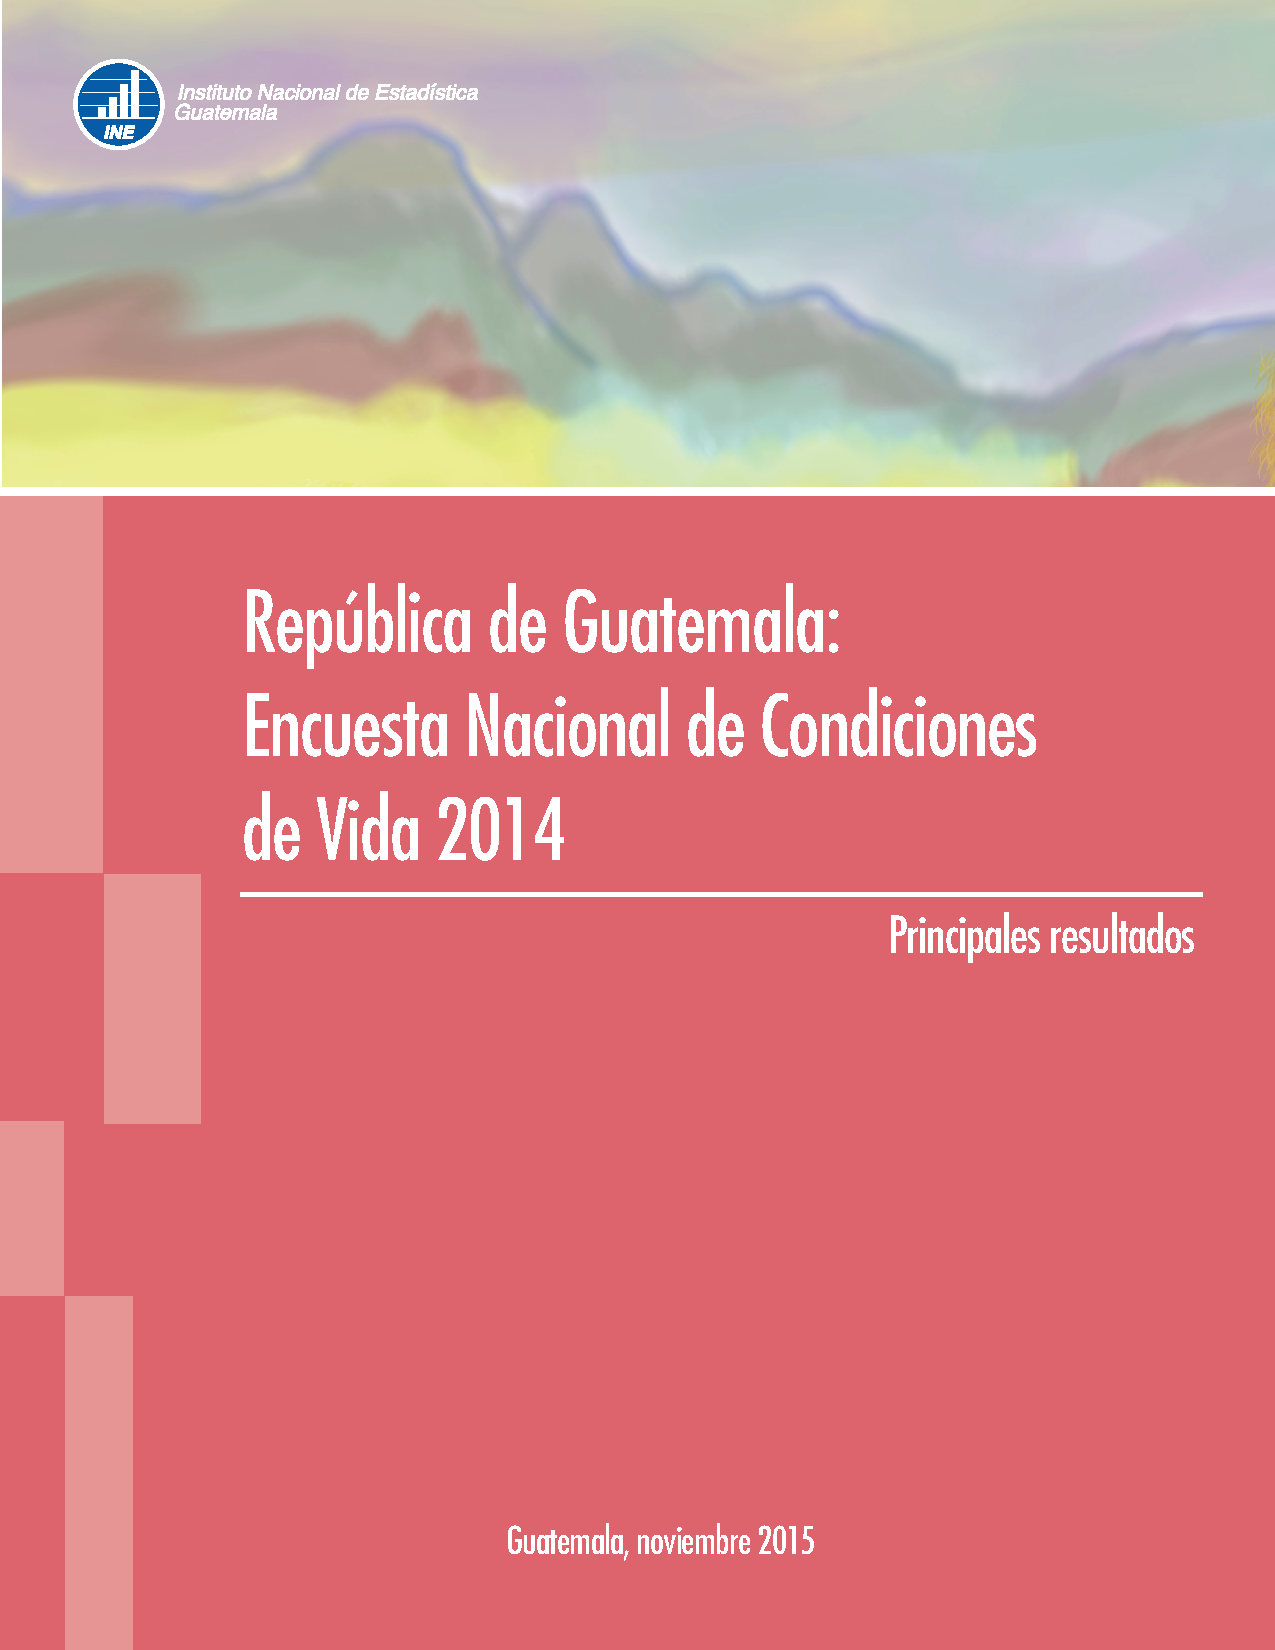
\includepdf{portada.pdf}
	\newpage
	\pagestyle{soloarriba}
\clearpage

$\ $
\vspace{14.5cm}

\noindent\begin{tabular}{p{0.9cm}p{6.8cm}}
& 2015.$\,$ Guatemala, Centro América \\
&\Bold Instituto Nacional de Estadística\\[-0.4cm]
&\color{blue!50!black}\url{www.ine.gob.gt}\\[0.9cm]
\end{tabular}\\
\noindent\begin{tabular}{p{0.9cm}p{6.8cm}}
& Está permitida la reproducción parcial o total de los contenidos de este documento con la mención de la fuente. \\[0.5cm]
 
& Este documento fue elaborado empleando  {\Sans R}, Inkscape y {\Logos \XeLaTeX}.\\
\end{tabular} 


\clearpage



	
	\clearpage
	\newpage $\ $

$\ $
\vspace{0.0cm}

\begin{center}
	{\Bold \LARGE AUTORIDADES}\\[1cm]
	
	
	{\Bold \large \color{color1!89!black} JUNTA  DIRECTIVA} \\[0.4cm]
	
	{ \Bold Ministerio de Economía}  		\\ 
	Titular: Jorge Méndez Herbruger   \\ 
	Suplente: Jacobo Rey Sigfrido Lee Leiva  \\ [0.4cm] 
	
	{\Bold Ministerio de Finanzas} \\ 
	Titular: Dorval José Carías Samayoa \\ 
	Suplente: Edwin Oswaldo Martínez Cameros\\[0.4cm] 
	
	{\Bold Ministerio de Agricultura, Ganadería y Alimentación} \\ 
	Titular: José Sebastian Marcucci Ruíz   \\ 
	Suplente: Henry Giovanni Vásquez Kilkan \\ [0.4cm] 
	
	{\Bold Ministerio de Energía y Minas}\\ 
	Titular: Juan Pablo Ligorría Arroyo \\ 
	Suplente: Jorge David Calvo Drago\\ [0.4cm]
	{\Bold Secretaría de Planificación y Programación de la Presidencia}   \\
	Titular: Ekaterina Arbolievna Parrilla Artuguina   \\ 
	Suplente: Dora Marina Coc Yup\\ [0.4cm] 
	{\Bold Banco de Guatemala} \\ 
	Titular: Julio Roberto Suárez Guerra \\ 
	Suplente: Sergio Francisco Recinos Rivera\\ [0.4cm] 
	{\Bold Universidad de San Carlos de Guatemala de Guatemala} \\ 
	Titular: Murphy Olimpo Paiz Recinos   \\
	Suplente: Oscar René Paniagua Carrera  \\ [0.4cm]
	{\Bold Universidades Privadas} \\
	Titular: Miguel Ángel Franco de León \\			 Suplente: Ariel Rivera Irías\\ [0.4cm] 
	{\Bold Comité Coordinador de \ Asociaciones  Agrícolas, Comerciales,Industriales y Financieras} \\ 
	Titular: Juan Raúl Aguilar Kaehler \\
	Suplente:  Oscar Augusto Sequeira García  \\ [0.4cm]
	
	{\Bold \large \color{color1!89!black} GERENCIA}\\[0.2cm]
	Gerente:  Rubén Darío Narciso Cruz		\\
	Subgerente Técnico:  Jaime Roberto Mejía Salguero\\
	Subgerente Administrativo Financiero:  Orlando Roberto Monzón Girón\\ 
\end{center}
\clearpage

$\ $
\vspace{1cm}

\begin{center}
	{\Bold \LARGE EQUIPO RESPONSABLE}\\[2cm]
	
	{\Bold \large \color{color1!89!black} REVISIÓN GENERAL}\\[0.2cm]
	Rubén Darío Narciso Cruz\\[0.8cm]
	
	
	{\Bold \large \color{color1!89!black} EQUIPO TÉCNICO}\\[0.2cm]
	Jaime Mejía\\
	Carlos Mancia\\
	Carlos Ortiz\\
	Marvin Reyes\\
	Hugo Rivas\\
	Nelson Santacruz \\
	Luis Fernando Bonilla\\
	Pamela Escobar\\
	Vivian Guzmán\\
	Patricia Hernández\\
	Sucely Donis \\
	Fabiola Ramírez \\
	Hugo García \\
	Mynor Flores \\[0.8cm]
	
{\Bold \large \color{color1!89!black} DIAGRAMACIÓN Y DISEÑO}\\[0.2cm]
Ligia Morales\\
José Carlos Bonilla Aldana
\end{center}
\vfill
\hrule 
El Instituto Nacional de Estadística agradece el apoyo técnico brindado por el Banco Mundial para la realización de esta encuesta; en especial a Carlos Sobrado,Mario Navarrete y  Elizaveta Perova por su valiosa contribución. 
\cleardoublepage
$\ $\\[2cm]
\noindent {\Bold \huge Presentación}
\\\\
 
 La Encuesta Nacional de Condiciones de Vida \textemdash Encovi\textemdash, tiene como principal objetivo, conocer y evaluar las condiciones de vida de la población, así como determinar los niveles de pobreza existentes en Guatemala y los factores que los determinan.
 
 La Encovi adopta la metodología de las encuestas de condiciones de vida, que en lo fundamental, combinan aspectos cuantitativos y cualitativos mediante la aplicación de un conjunto integrado de formularios sobre la calidad de vida de los hogares y las personas. Esta perspectiva permite una mejor aproximación a los diferentes aspectos y componentes de la pobreza, es decir, a su carácter multidimensional. Permite además, abordar el estudio de la desigualdad y la identificación de mecanismos de intervención eficaz que promuevan mejoras sustantivas de las condiciones de vida.

Debido a la amplitud de los temas investigados en la Encovi, el informe de resultados de esta encuesta se presentará en tres tomos en el 2016. Sin embargo, para que la población en general tenga oportunamente    los principales resultados de la Encovi 2014, se presenta este informe, el cúal es un extracto del documento de mayor volumen que se publicará el próximo año.  El presente documento tiene tres capítulos: Pobreza, Desigualdad y Objetivos de Desarrollo del Milenio, los que permiten visualizar la evolución de las condiciones de vida del país en los últimos quince años. 


El Instituto Nacional de Estadística agradece a todas las instituciones públicas, privadas y de cooperación internacional que apoyaron este esfuerzo. Asimismo, a los hogares que abrieron sus puertas y  brindaron  la información  solicitada, sin la cual no hubiera sido posible  la elaboración de este informe.\\[1cm] 


\begin{center}
	\textbf{Rubén Darío Narciso Cruz}\\
	Gerente\\
	Instituto Nacional de Estadística
\end{center}

\cleardoublepage


	\tableofcontents
	\pagestyle{estandar}
	\setcounter{page}{0}
	




%
 \cajita{%
Línea de pobreza total }%
{%
  Para el año 2000, el valor de la línea de pobreza total\footnote{La línea de pobreza total incluye, además del costo alimenticio, un monto adicional que corresponde al porcentaje de consumo no alimenticio de las personas, cuyo consumo de alimentos se encuentra alrededor de la línea de pobreza extrema.} era de Q 4,319\footnote{ Este valor ajustado a precios de 2014  equivale a 10,000  quetzales. }.
 
  Se puede observar que para 2014, el costo de alimentación más bienes y servicios, aumentó a Q 10,218 lo que equivale a un incremento del 137\% .}%
{%
 Líneas de pobreza total nacional} %
{%
 Républica de Guatemala, Encovi 2000, 2006 y 2014, en quetzales de cada año} %
{%
 \begin{tikzpicture}[x=1pt,y=1pt]  % Created by tikzDevice version 0.7.0 on 2015-11-27 11:12:31
% !TEX encoding = UTF-8 Unicode
\definecolor[named]{fillColor}{rgb}{1.00,1.00,1.00}
\path[use as bounding box,fill=fillColor,fill opacity=0.00] (0,0) rectangle (289.08,198.74);
\begin{scope}
\path[clip] (  0.00,  0.00) rectangle (289.08,198.74);

\path[] (  0.00,  0.00) rectangle (289.08,198.74);
\end{scope}
\begin{scope}
\path[clip] (  0.00,  0.00) rectangle (289.08,198.74);

\path[] ( 14.78, 17.78) rectangle (280.54,191.48);

\path[] ( 14.78, 34.98) --
	(280.54, 34.98);

\path[] ( 14.78, 76.15) --
	(280.54, 76.15);

\path[] ( 14.78,117.33) --
	(280.54,117.33);

\path[] ( 14.78,158.51) --
	(280.54,158.51);

\path[] ( 14.78, 55.57) --
	(280.54, 55.57);

\path[] ( 14.78, 96.74) --
	(280.54, 96.74);

\path[] ( 14.78,137.92) --
	(280.54,137.92);

\path[] ( 14.78,179.10) --
	(280.54,179.10);

\path[] ( 64.61, 17.78) --
	( 64.61,191.48);

\path[] (147.66, 17.78) --
	(147.66,191.48);

\path[] (230.71, 17.78) --
	(230.71,191.48);
\definecolor[named]{drawColor}{rgb}{0.00,0.00,1.00}

\path[draw=drawColor,line width= 1.7pt,line join=round] ( 64.61, 62.11) --
	(147.66,108.56) --
	(230.71,183.59);
\definecolor[named]{drawColor}{rgb}{0.00,0.00,0.00}

\node[text=drawColor,anchor=base,inner sep=0pt, outer sep=0pt, scale=  1.01] at ( 64.61, 50.24) {4,318};

\node[text=drawColor,anchor=base east,inner sep=0pt, outer sep=0pt, scale=  1.01] at (143.66,108.56) {6,574};

\node[text=drawColor,anchor=base,inner sep=0pt, outer sep=0pt, scale=  1.01] at (230.71,187.54) {10,218};
\definecolor[named]{fillColor}{rgb}{0.00,0.00,0.00}

\path[draw=drawColor,line width= 0.1pt,line join=round,fill=fillColor] ( 14.78, 25.67) -- (280.54, 25.67);

\path[] ( 14.78, 17.78) rectangle (280.54,191.48);
\end{scope}
\begin{scope}
\path[clip] (  0.00,  0.00) rectangle (289.08,198.74);

\path[] ( 14.78, 17.78) --
	( 14.78,191.48);
\end{scope}
\begin{scope}
\path[clip] (  0.00,  0.00) rectangle (289.08,198.74);
\definecolor[named]{drawColor}{rgb}{1.00,1.00,1.00}

\node[text=drawColor,text opacity=0.00,anchor=base east,inner sep=0pt, outer sep=0pt, scale=  1.00] at (  7.67, 51.66) {4000};

\node[text=drawColor,text opacity=0.00,anchor=base east,inner sep=0pt, outer sep=0pt, scale=  1.00] at (  7.67, 92.84) {6000};

\node[text=drawColor,text opacity=0.00,anchor=base east,inner sep=0pt, outer sep=0pt, scale=  1.00] at (  7.67,134.01) {8000};

\node[text=drawColor,text opacity=0.00,anchor=base east,inner sep=0pt, outer sep=0pt, scale=  1.00] at (  7.67,175.19) {10000};
\end{scope}
\begin{scope}
\path[clip] (  0.00,  0.00) rectangle (289.08,198.74);

\path[] ( 10.51, 55.57) --
	( 14.78, 55.57);

\path[] ( 10.51, 96.74) --
	( 14.78, 96.74);

\path[] ( 10.51,137.92) --
	( 14.78,137.92);

\path[] ( 10.51,179.10) --
	( 14.78,179.10);
\end{scope}
\begin{scope}
\path[clip] (  0.00,  0.00) rectangle (289.08,198.74);

\path[] ( 14.78, 17.78) --
	(280.54, 17.78);
\end{scope}
\begin{scope}
\path[clip] (  0.00,  0.00) rectangle (289.08,198.74);

\path[] ( 64.61, 13.51) --
	( 64.61, 17.78);

\path[] (147.66, 13.51) --
	(147.66, 17.78);

\path[] (230.71, 13.51) --
	(230.71, 17.78);
\end{scope}
\begin{scope}
\path[clip] (  0.00,  0.00) rectangle (289.08,198.74);
\definecolor[named]{drawColor}{rgb}{0.00,0.00,0.00}

\node[text=drawColor,anchor=base,inner sep=0pt, outer sep=0pt, scale=  1.00] at ( 64.61,  2.85) {2000};

\node[text=drawColor,anchor=base,inner sep=0pt, outer sep=0pt, scale=  1.00] at (147.66,  2.85) {2006};

\node[text=drawColor,anchor=base,inner sep=0pt, outer sep=0pt, scale=  1.00] at (230.71,  2.85) {2014};
\end{scope}
  \end{tikzpicture}}%
{%
 Instituto Nacional de Estadística} %
 
 \cajita{%
Pobreza total}%
{%
 Trae fórmula Nota: indicador FGT (Foster, Greer y Thorbecke) Para 2014, el 59.3\% de la población se encontraba por debajo de la línea de pobreza total, es decir, más de la mitad de la población tenía un consumo por debajo de Q10,218 al año. Se puede observar en la gráfica  que entre 2000 y 2014, la pobreza total aumentó en 2.9 puntos porcentuales, pasando de 56.4\% en 2000 a 59.3\% en 2014.}%
{%
 Incidencia de pobreza total nacional} %
{%
 Républica de Guatemala, serie histórica por Encovi, en porcentaje} %
{%
 \begin{tikzpicture}[x=1pt,y=1pt]  % Created by tikzDevice version 0.7.0 on 2015-11-27 11:12:32
% !TEX encoding = UTF-8 Unicode
\definecolor[named]{fillColor}{rgb}{1.00,1.00,1.00}
\path[use as bounding box,fill=fillColor,fill opacity=0.00] (0,0) rectangle (289.08,198.74);
\begin{scope}
\path[clip] (  0.00,  0.00) rectangle (289.08,198.74);

\path[] (  0.00,  0.00) rectangle (289.08,198.74);
\end{scope}
\begin{scope}
\path[clip] (  0.00,  0.00) rectangle (289.08,198.74);

\path[] (  1.64, 17.78) rectangle (280.54,191.48);

\path[] (  1.64, 37.36) --
	(280.54, 37.36);

\path[] (  1.64, 82.20) --
	(280.54, 82.20);

\path[] (  1.64,127.03) --
	(280.54,127.03);

\path[] (  1.64,171.86) --
	(280.54,171.86);

\path[] (  1.64, 59.78) --
	(280.54, 59.78);

\path[] (  1.64,104.61) --
	(280.54,104.61);

\path[] (  1.64,149.44) --
	(280.54,149.44);

\path[] ( 53.94, 17.78) --
	( 53.94,191.48);

\path[] (141.09, 17.78) --
	(141.09,191.48);

\path[] (228.25, 17.78) --
	(228.25,191.48);
\definecolor[named]{drawColor}{rgb}{0.00,0.00,1.00}

\path[draw=drawColor,line width= 1.7pt,line join=round] ( 53.94,140.63) --
	(141.09, 62.11) --
	(228.25,183.59);
\definecolor[named]{drawColor}{rgb}{0.00,0.00,0.00}

\node[text=drawColor,anchor=base,inner sep=0pt, outer sep=0pt, scale=  1.01] at ( 53.94,144.58) {56.4};

\node[text=drawColor,anchor=base,inner sep=0pt, outer sep=0pt, scale=  1.01] at (141.09, 50.24) {51.2};

\node[text=drawColor,anchor=base,inner sep=0pt, outer sep=0pt, scale=  1.01] at (228.25,187.54) {59.3};
\definecolor[named]{fillColor}{rgb}{0.00,0.00,0.00}

\path[draw=drawColor,line width= 0.1pt,line join=round,fill=fillColor] (  1.64, 25.67) -- (280.54, 25.67);

\path[] (  1.64, 17.78) rectangle (280.54,191.48);
\end{scope}
\begin{scope}
\path[clip] (  0.00,  0.00) rectangle (289.08,198.74);

\path[] (  1.64, 17.78) --
	(  1.64,191.48);
\end{scope}
\begin{scope}
\path[clip] (  0.00,  0.00) rectangle (289.08,198.74);

\path[] (  0.00, 59.78) --
	(  1.64, 59.78);

\path[] (  0.00,104.61) --
	(  1.64,104.61);

\path[] (  0.00,149.44) --
	(  1.64,149.44);
\end{scope}
\begin{scope}
\path[clip] (  0.00,  0.00) rectangle (289.08,198.74);

\path[] (  1.64, 17.78) --
	(280.54, 17.78);
\end{scope}
\begin{scope}
\path[clip] (  0.00,  0.00) rectangle (289.08,198.74);

\path[] ( 53.94, 13.51) --
	( 53.94, 17.78);

\path[] (141.09, 13.51) --
	(141.09, 17.78);

\path[] (228.25, 13.51) --
	(228.25, 17.78);
\end{scope}
\begin{scope}
\path[clip] (  0.00,  0.00) rectangle (289.08,198.74);
\definecolor[named]{drawColor}{rgb}{0.00,0.00,0.00}

\node[text=drawColor,anchor=base,inner sep=0pt, outer sep=0pt, scale=  1.00] at ( 53.94,  2.85) {2000};

\node[text=drawColor,anchor=base,inner sep=0pt, outer sep=0pt, scale=  1.00] at (141.09,  2.85) {2006};

\node[text=drawColor,anchor=base,inner sep=0pt, outer sep=0pt, scale=  1.00] at (228.25,  2.85) {2014};
\end{scope}
  \end{tikzpicture}}%
{%
 Instituto Nacional de Estadística} %
 
 \cajita{%
Pobreza total por etnicidad}%
{%
 Para 2014, casi cuatro de cada cinco personas indígenas se encontraba en pobreza. Al comparar los niveles de pobreza con la población no indígena, se obtiene que la pobreza en la población indígena era 1.7 veces mayor que en la población no indígena. Se puede observar que entre 2000 y 2014, hubo un aumento de la pobreza para ambos grupos, aunque el aumento fue mayor en la población no indígena que en la población indígena, 4.7 y 1.9 puntos porcentuales, respectivamente.}%
{%
 Incidencia de pobreza total por etnicidad} %
{%
 Républica de Guatemala, serie histórica por Encovi, en porcentaje} %
{%
 \begin{tikzpicture}[x=1pt,y=1pt]  % Created by tikzDevice version 0.9 on 2015-12-01 14:57:19
% !TEX encoding = UTF-8 Unicode
\definecolor{fillColor}{RGB}{255,255,255}
\path[use as bounding box,fill=fillColor,fill opacity=0.00] (0,0) rectangle (289.08,198.74);
\begin{scope}
\path[clip] (  0.00,  0.00) rectangle (289.08,198.74);

\path[] (  0.00,  0.00) rectangle (289.08,198.74);
\end{scope}
\begin{scope}
\path[clip] (  0.00,  0.00) rectangle (289.08,198.74);

\path[] (  7.11, 20.62) rectangle (289.08,172.42);

\path[] ( 59.98, 20.62) --
	( 59.98,172.42);

\path[] (148.10, 20.62) --
	(148.10,172.42);

\path[] (236.21, 20.62) --
	(236.21,172.42);
\definecolor{drawColor}{RGB}{0,0,255}
\definecolor{fillColor}{RGB}{0,0,255}

\path[draw=drawColor,line width= 0.6pt,line join=round,fill=fillColor] ( 26.94, 20.62) rectangle ( 53.37,168.70);
\definecolor{drawColor}{RGB}{157,187,255}
\definecolor{fillColor}{RGB}{157,187,255}

\path[draw=drawColor,line width= 0.6pt,line join=round,fill=fillColor] ( 66.59, 20.62) rectangle ( 93.02,100.90);
\definecolor{drawColor}{RGB}{0,0,255}
\definecolor{fillColor}{RGB}{0,0,255}

\path[draw=drawColor,line width= 0.6pt,line join=round,fill=fillColor] (115.05, 20.62) rectangle (141.49,164.31);
\definecolor{drawColor}{RGB}{157,187,255}
\definecolor{fillColor}{RGB}{157,187,255}

\path[draw=drawColor,line width= 0.6pt,line join=round,fill=fillColor] (154.71, 20.62) rectangle (181.14, 90.23);
\definecolor{drawColor}{RGB}{0,0,255}
\definecolor{fillColor}{RGB}{0,0,255}

\path[draw=drawColor,line width= 0.6pt,line join=round,fill=fillColor] (203.17, 20.62) rectangle (229.60,172.42);
\definecolor{drawColor}{RGB}{157,187,255}
\definecolor{fillColor}{RGB}{157,187,255}

\path[draw=drawColor,line width= 0.6pt,line join=round,fill=fillColor] (242.82, 20.62) rectangle (269.25,109.86);
\definecolor{drawColor}{RGB}{0,0,0}

\path[draw=drawColor,line width= 0.6pt,line join=round] (  7.11, 20.62) -- (289.08, 20.62);

\node[text=drawColor,anchor=base,inner sep=0pt, outer sep=0pt, scale=  0.82] at ( 40.16,171.92) {77.3};

\node[text=drawColor,anchor=base,inner sep=0pt, outer sep=0pt, scale=  0.82] at ( 79.81,104.13) {41.9};

\node[text=drawColor,anchor=base,inner sep=0pt, outer sep=0pt, scale=  0.82] at (128.27,167.53) {75.0};

\node[text=drawColor,anchor=base,inner sep=0pt, outer sep=0pt, scale=  0.82] at (167.92, 93.45) {36.3};

\node[text=drawColor,anchor=base,inner sep=0pt, outer sep=0pt, scale=  0.82] at (216.39,175.65) {79.2};

\node[text=drawColor,anchor=base,inner sep=0pt, outer sep=0pt, scale=  0.82] at (256.04,113.08) {46.6};

\path[] (  7.11, 20.62) rectangle (289.08,172.42);
\end{scope}
\begin{scope}
\path[clip] (  0.00,  0.00) rectangle (289.08,198.74);

\path[] (  7.11, 20.62) --
	(  7.11,172.42);
\end{scope}
\begin{scope}
\path[clip] (  0.00,  0.00) rectangle (289.08,198.74);

\path[] (  7.11, 20.62) --
	(289.08, 20.62);
\end{scope}
\begin{scope}
\path[clip] (  0.00,  0.00) rectangle (289.08,198.74);

\path[] ( 59.98, 16.35) --
	( 59.98, 20.62);

\path[] (148.10, 16.35) --
	(148.10, 20.62);

\path[] (236.21, 16.35) --
	(236.21, 20.62);
\end{scope}
\begin{scope}
\path[clip] (  0.00,  0.00) rectangle (289.08,198.74);
\definecolor{drawColor}{RGB}{0,0,0}

\node[text=drawColor,anchor=base,inner sep=0pt, outer sep=0pt, scale=  1.00] at ( 59.98,  5.69) {2000};

\node[text=drawColor,anchor=base,inner sep=0pt, outer sep=0pt, scale=  1.00] at (148.10,  5.69) {2006};

\node[text=drawColor,anchor=base,inner sep=0pt, outer sep=0pt, scale=  1.00] at (236.21,  5.69) {2014};
\end{scope}
\begin{scope}
\path[clip] (  0.00,  0.00) rectangle (289.08,198.74);
\coordinate (apoyo) at (55.19,188.79);
\coordinate (longitudFicticia) at (7.11,9.95);
\coordinate (longitud) at (7.11,7.11);
\coordinate (desX) at (133.24,0);
\coordinate (desY) at (0,1.42);
\definecolor[named]{ct1}{HTML}{
0000FF
}
\definecolor[named]{ct2}{HTML}{
9DBBFF
}
\definecolor[named]{ctb1}{HTML}{
0000FF
}
\definecolor[named]{ctb2}{HTML}{
9DBBFF
}
\path [fill=none] (apoyo) rectangle ($(apoyo)+(longitudFicticia)$)
node [xshift=0.3cm,inner sep=0pt, outer sep=0pt,midway,right,scale = 0.9]{Indígena};
\draw [color = ctb1,fill=ct1] ( $(apoyo)  + (desY) $) rectangle ($(apoyo)+ (desY) +(longitud)$);
\path [fill=none] ($(apoyo)+(desX)$) rectangle ($(apoyo)+(desX)+(longitudFicticia)$)
node [xshift=0.3cm,inner sep=0pt, outer sep=0pt,midway,right,scale = 0.9]{No indígena};
\draw [color = ctb2 ,fill=ct2] ( $(apoyo)  + (desY) + (desX) $) rectangle ($(apoyo)+ (desY)+ (desX) +(longitud)$);
\end{scope}
  \end{tikzpicture}}%
{%
 Instituto Nacional de Estadística} %
 
 \cajita{%
Pobreza total por área de residencia}%
{%
 Según las estimaciones de pobreza, entre 2000 y 2014 hubo un aumento de la pobreza, tanto en el área urbana como en el área rural, siendo superior la pobreza en el área rural.  En la gráfica se advierte que la brecha entre la pobreza en el área urbana y el área rural se ha ido reduciendo en este período, ya que para el año 2000 la pobreza en el área rural era 2.7 veces mayor que en el área urbana, y para 2014 se redujo a 1.8. }%
{%
 Incidencia de pobreza total por área de residencia} %
{%
 Républica de Guatemala, serie histórica por Encovi, en porcentaje} %
{%
 \begin{tikzpicture}[x=1pt,y=1pt]  % Created by tikzDevice version 0.9 on 2015-11-26 21:53:05
% !TEX encoding = UTF-8 Unicode
\definecolor{fillColor}{RGB}{255,255,255}
\path[use as bounding box,fill=fillColor,fill opacity=0.00] (0,0) rectangle (289.08,198.74);
\begin{scope}
\path[clip] (  0.00,  0.00) rectangle (289.08,198.74);

\path[] (  0.00,  0.00) rectangle (289.08,198.74);
\end{scope}
\begin{scope}
\path[clip] (  0.00,  0.00) rectangle (289.08,198.74);

\path[] (  7.11, 20.62) rectangle (289.08,172.42);

\path[] ( 47.39, 20.62) --
	( 47.39,172.42);

\path[] (114.53, 20.62) --
	(114.53,172.42);

\path[] (181.66, 20.62) --
	(181.66,172.42);

\path[] (248.80, 20.62) --
	(248.80,172.42);
\definecolor{drawColor}{RGB}{0,0,255}
\definecolor{fillColor}{RGB}{0,0,255}

\path[draw=drawColor,line width= 0.6pt,line join=round,fill=fillColor] ( 18.86, 20.62) rectangle ( 45.72,172.42);
\definecolor{drawColor}{RGB}{157,187,255}
\definecolor{fillColor}{RGB}{157,187,255}

\path[draw=drawColor,line width= 0.6pt,line join=round,fill=fillColor] ( 49.07, 20.62) rectangle ( 75.93,102.92);
\definecolor{drawColor}{RGB}{0,0,255}
\definecolor{fillColor}{RGB}{0,0,255}

\path[draw=drawColor,line width= 0.6pt,line join=round,fill=fillColor] ( 86.00, 20.62) rectangle (112.85,167.92);
\definecolor{drawColor}{RGB}{157,187,255}
\definecolor{fillColor}{RGB}{157,187,255}

\path[draw=drawColor,line width= 0.6pt,line join=round,fill=fillColor] (116.21, 20.62) rectangle (143.06, 91.98);
\definecolor{drawColor}{RGB}{0,0,255}
\definecolor{fillColor}{RGB}{0,0,255}

\path[draw=drawColor,line width= 0.6pt,line join=round,fill=fillColor] (153.13, 20.62) rectangle (179.99,164.83);
\definecolor{drawColor}{RGB}{157,187,255}
\definecolor{fillColor}{RGB}{157,187,255}

\path[draw=drawColor,line width= 0.6pt,line join=round,fill=fillColor] (183.34, 20.62) rectangle (210.20,100.35);
\definecolor{drawColor}{RGB}{0,0,255}
\definecolor{fillColor}{RGB}{0,0,255}

\path[draw=drawColor,line width= 0.6pt,line join=round,fill=fillColor] (220.27, 20.62) rectangle (247.12, 20.62);
\definecolor{drawColor}{RGB}{157,187,255}
\definecolor{fillColor}{RGB}{157,187,255}

\path[draw=drawColor,line width= 0.6pt,line join=round,fill=fillColor] (250.48, 20.62) rectangle (277.33, 20.62);
\definecolor{drawColor}{RGB}{0,0,0}

\path[draw=drawColor,line width= 0.6pt,line join=round] (  7.11, 20.62) -- (289.08, 20.62);

\node[text=drawColor,anchor=base,inner sep=0pt, outer sep=0pt, scale=  0.82] at ( 32.29,175.65) {77.3};

\node[text=drawColor,anchor=base,inner sep=0pt, outer sep=0pt, scale=  0.82] at ( 62.50,106.15) {41.9};

\node[text=drawColor,anchor=base,inner sep=0pt, outer sep=0pt, scale=  0.82] at ( 99.42,171.15) {75.0};

\node[text=drawColor,anchor=base,inner sep=0pt, outer sep=0pt, scale=  0.82] at (129.63, 95.20) {36.3};

\node[text=drawColor,anchor=base,inner sep=0pt, outer sep=0pt, scale=  0.82] at (166.56,168.05) {73.4};

\node[text=drawColor,anchor=base,inner sep=0pt, outer sep=0pt, scale=  0.82] at (196.77,103.57) {40.6};

\node[text=drawColor,anchor=base,inner sep=0pt, outer sep=0pt, scale=  0.82] at (233.69, 23.84) {0.0};

\node[text=drawColor,anchor=base,inner sep=0pt, outer sep=0pt, scale=  0.82] at (263.90, 23.84) {0.0};

\path[] (  7.11, 20.62) rectangle (289.08,172.42);
\end{scope}
\begin{scope}
\path[clip] (  0.00,  0.00) rectangle (289.08,198.74);

\path[] (  7.11, 20.62) --
	(  7.11,172.42);
\end{scope}
\begin{scope}
\path[clip] (  0.00,  0.00) rectangle (289.08,198.74);

\path[] (  7.11, 20.62) --
	(289.08, 20.62);
\end{scope}
\begin{scope}
\path[clip] (  0.00,  0.00) rectangle (289.08,198.74);

\path[] ( 47.39, 16.35) --
	( 47.39, 20.62);

\path[] (114.53, 16.35) --
	(114.53, 20.62);

\path[] (181.66, 16.35) --
	(181.66, 20.62);

\path[] (248.80, 16.35) --
	(248.80, 20.62);
\end{scope}
\begin{scope}
\path[clip] (  0.00,  0.00) rectangle (289.08,198.74);
\definecolor{drawColor}{RGB}{0,0,0}

\node[text=drawColor,anchor=base,inner sep=0pt, outer sep=0pt, scale=  1.00] at ( 47.39,  5.69) {2000};

\node[text=drawColor,anchor=base,inner sep=0pt, outer sep=0pt, scale=  1.00] at (114.53,  5.69) {2006};

\node[text=drawColor,anchor=base,inner sep=0pt, outer sep=0pt, scale=  1.00] at (181.66,  5.69) {2011};

\node[text=drawColor,anchor=base,inner sep=0pt, outer sep=0pt, scale=  1.00] at (248.80,  5.69) {2014};
\end{scope}
\begin{scope}
\path[clip] (  0.00,  0.00) rectangle (289.08,198.74);
\coordinate (apoyo) at (55.19,188.79);
\coordinate (longitudFicticia) at (7.11,9.95);
\coordinate (longitud) at (7.11,7.11);
\coordinate (desX) at (133.24,0);
\coordinate (desY) at (0,1.42);
\definecolor[named]{ct1}{HTML}{
0000FF
}
\definecolor[named]{ct2}{HTML}{
9DBBFF
}
\definecolor[named]{ctb1}{HTML}{
0000FF
}
\definecolor[named]{ctb2}{HTML}{
9DBBFF
}
\path [fill=none] (apoyo) rectangle ($(apoyo)+(longitudFicticia)$)
node [xshift=0.3cm,inner sep=0pt, outer sep=0pt,midway,right,scale = 0.9]{Indígena};
\draw [color = ctb1,fill=ct1] ( $(apoyo)  + (desY) $) rectangle ($(apoyo)+ (desY) +(longitud)$);
\path [fill=none] ($(apoyo)+(desX)$) rectangle ($(apoyo)+(desX)+(longitudFicticia)$)
node [xshift=0.3cm,inner sep=0pt, outer sep=0pt,midway,right,scale = 0.9]{No indígena};
\draw [color = ctb2 ,fill=ct2] ( $(apoyo)  + (desY) + (desX) $) rectangle ($(apoyo)+ (desY)+ (desX) +(longitud)$);
\end{scope}
  \end{tikzpicture}}%
{%
 Instituto Nacional de Estadística} %
 
 \cajota{%
Pobreza total en los departamentos en 2006}%
{%
 Para 2006, los departamentos de Quiché, Alta Verapaz y Sololá, mostraban los porcentajes de pobreza más altos, con 81.0\%, 78.8\% y 74.6\%, respectivamente. Escuintla y el Progreso presentaban poco más de la mitad de la pobreza observada en Quiché. 

Asimismo, los departamentos con los niveles más bajos de pobreza eran Sacatepéquez con 36.5\% y Guatemala con  16.3\%, }%
{%
 Incidencia de pobreza total por departamento 2006} %
{%
 República de Guatemala, Encovi 2016 en porcentaje} %
{%
 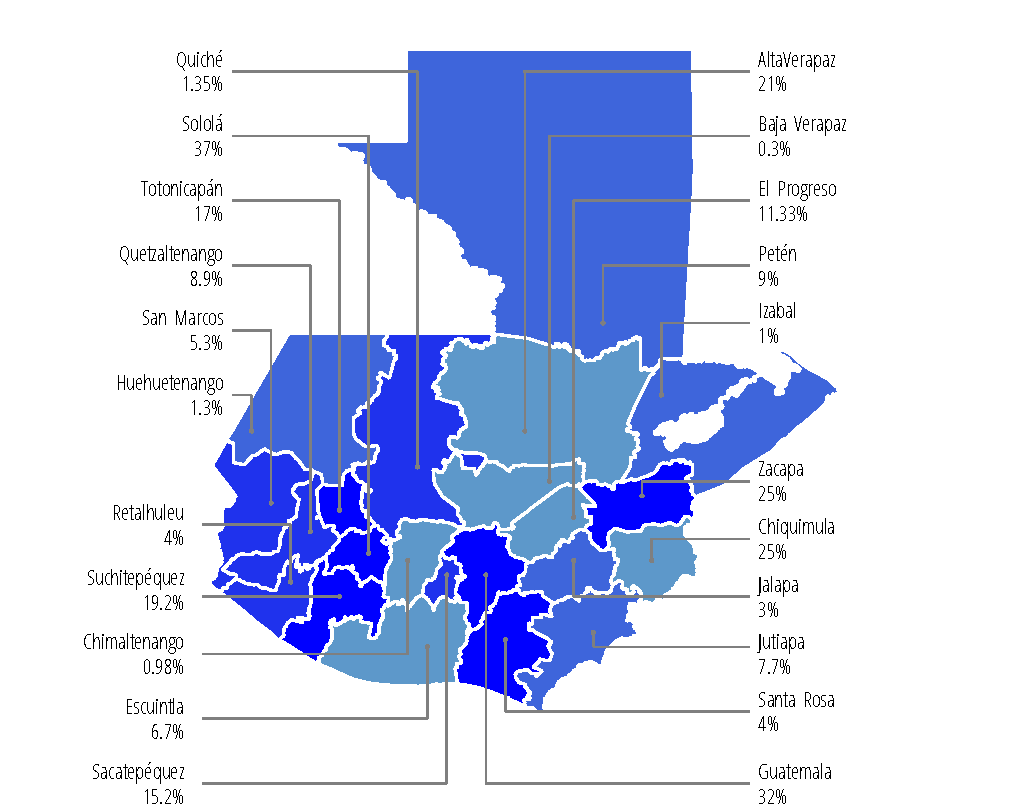
\includegraphics[width=52\cuadri]{graficas/1_05.pdf}}%
{%
 Instituto Nacional de Estadística} %
 
 \cajota{%
Pobreza total en los departamentos en 2014}%
{%
 La línea de pobreza extrema representa el costo de adquirir la cantidad mínima de calorías recomendadas. Para el año 2000, la línea de pobreza era de 1,911 quetzales, que ajustado a precios de 2014, era equivalente a Q4,427. La línea de pobreza para 2006, ajustada a 2014 era equivalente a 4,380 quetzales. Esto quiere decir que aproximadamente la línea de pobreza extrema aumentó en 1,370 quetzales entre 2006 y 2014.  }%
{%
 Incidencia de pobreza total por departamento 2014} %
{%
 Por departamento, Encovi 2014, en porcentaje} %
{%
 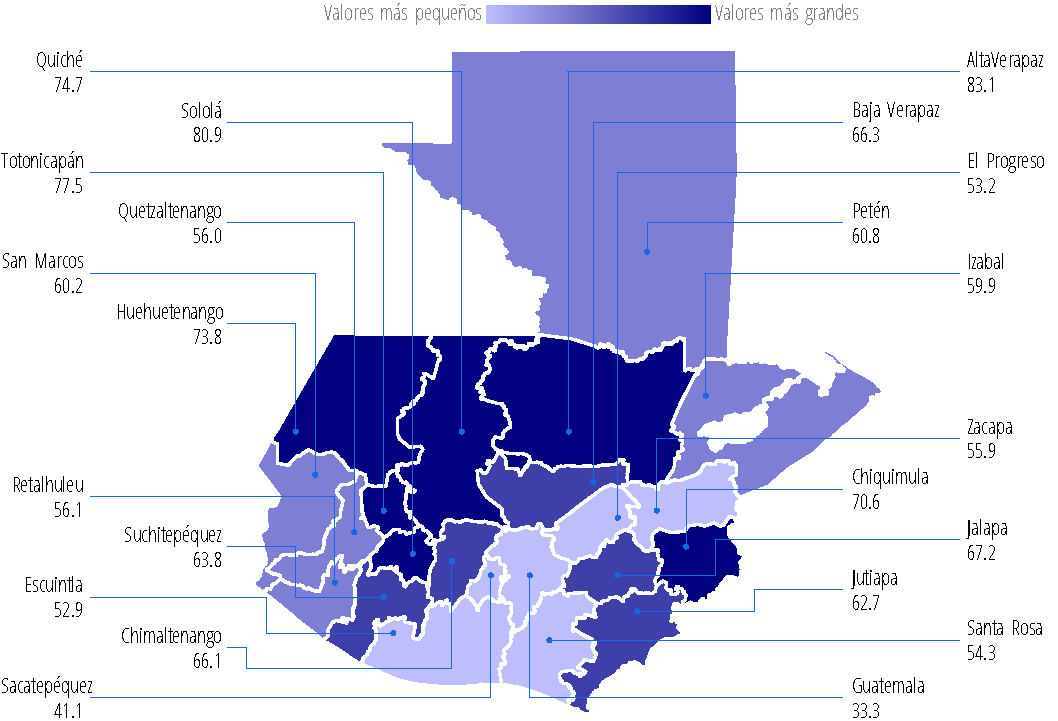
\includegraphics[width=52\cuadri]{graficas/1_06.pdf}}%
{%
 Instituto Nacional de Estadística} %
 
 \cajota{%
Cambio de la pobreza total }%
{%
 Los resultados positivos de la comparación entre 2006 y 2014, significan un aumento de la pobreza en este período. Se puede observar que el mayor aumento entre estos dos años, se dio en el departamento de Guatemala, con un aumento de 17 puntos porcentuales en la pobreza. Le siguen los departamentos de Jutiapa, Quetzaltenango, Escuintla, El Progreso y Chiquimula, con un aumento de más de 10 puntos porcentuales. Los departamentos que muestran una reducción de la pobreza son Quiché, San Marcos, Baja Verapaz y Santa Rosa. }%
{%
 Incidencia de pobreza extrema nacional} %
{%
 Por departamento, Encovi 2006 y 2014, en puntos porcentuales} %
{%
 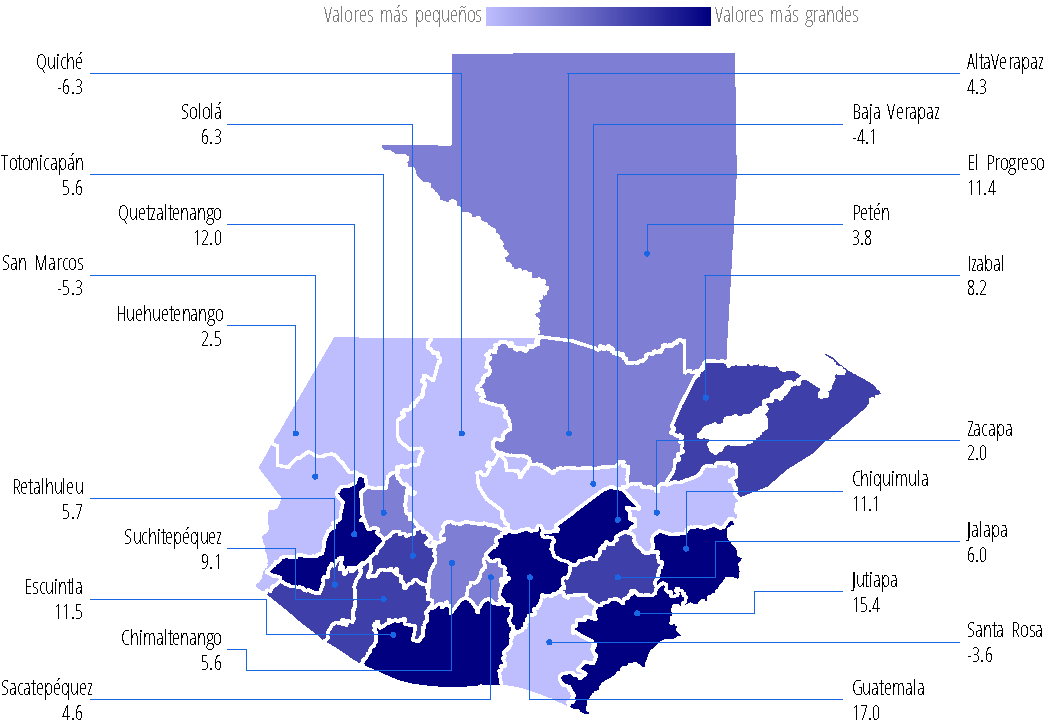
\includegraphics[width=52\cuadri]{graficas/1_07.pdf}}%
{%
 Instituto Nacional de Estadística} %
 
 \cajita{%
Línea de pobreza extrema}%
{%
 La pobreza extrema es mayor en la población indígena. Para el año 2000, más de la cuarta parte de la población indígena se encontraba en pobreza extrema, se puede observar que entre 2000 y 2006 el nivel de pobreza se mantuvo, y aumentó a casi 40\% en 2014. Para la población no indígena, la pobreza extrema aumentó de cinco puntos porcentuales, de 7.8\% a 12.8\% entre 2000 y 2014.}%
{%
 Líneas de pobreza extrema nacional} %
{%
 Républica de Guatemala, Encovi 2000, 2006 y 2014, en quetzales de cada año} %
{%
 \begin{tikzpicture}[x=1pt,y=1pt]  % Created by tikzDevice version 0.9 on 2015-11-26 21:53:16
% !TEX encoding = UTF-8 Unicode
\definecolor{fillColor}{RGB}{255,255,255}
\path[use as bounding box,fill=fillColor,fill opacity=0.00] (0,0) rectangle (289.08,198.74);
\begin{scope}
\path[clip] (  0.00,  0.00) rectangle (289.08,198.74);

\path[] (  0.00,  0.00) rectangle (289.08,198.74);
\end{scope}
\begin{scope}
\path[clip] (  0.00,  0.00) rectangle (289.08,198.74);

\path[] (  7.11, 20.62) rectangle (289.08,174.77);

\path[] ( 47.39, 20.62) --
	( 47.39,174.77);

\path[] (114.53, 20.62) --
	(114.53,174.77);

\path[] (181.66, 20.62) --
	(181.66,174.77);

\path[] (248.80, 20.62) --
	(248.80,174.77);
\definecolor{drawColor}{RGB}{0,0,255}
\definecolor{fillColor}{RGB}{0,0,255}

\path[draw=drawColor,line width= 0.6pt,line join=round,fill=fillColor] ( 18.86, 20.62) rectangle ( 45.72, 38.49);
\definecolor{drawColor}{RGB}{157,187,255}
\definecolor{fillColor}{RGB}{157,187,255}

\path[draw=drawColor,line width= 0.6pt,line join=round,fill=fillColor] ( 49.07, 20.62) rectangle ( 75.93,170.52);
\definecolor{drawColor}{RGB}{0,0,255}
\definecolor{fillColor}{RGB}{0,0,255}

\path[draw=drawColor,line width= 0.6pt,line join=round,fill=fillColor] ( 86.00, 20.62) rectangle (112.85, 54.27);
\definecolor{drawColor}{RGB}{157,187,255}
\definecolor{fillColor}{RGB}{157,187,255}

\path[draw=drawColor,line width= 0.6pt,line join=round,fill=fillColor] (116.21, 20.62) rectangle (143.06,174.77);
\definecolor{drawColor}{RGB}{0,0,255}
\definecolor{fillColor}{RGB}{0,0,255}

\path[draw=drawColor,line width= 0.6pt,line join=round,fill=fillColor] (153.13, 20.62) rectangle (179.99, 52.58);
\definecolor{drawColor}{RGB}{157,187,255}
\definecolor{fillColor}{RGB}{157,187,255}

\path[draw=drawColor,line width= 0.6pt,line join=round,fill=fillColor] (183.34, 20.62) rectangle (210.20,153.85);
\definecolor{drawColor}{RGB}{0,0,255}
\definecolor{fillColor}{RGB}{0,0,255}

\path[draw=drawColor,line width= 0.6pt,line join=round,fill=fillColor] (220.27, 20.62) rectangle (247.12, 20.62);
\definecolor{drawColor}{RGB}{157,187,255}
\definecolor{fillColor}{RGB}{157,187,255}

\path[draw=drawColor,line width= 0.6pt,line join=round,fill=fillColor] (250.48, 20.62) rectangle (277.33, 20.62);
\definecolor{drawColor}{RGB}{0,0,0}

\path[draw=drawColor,line width= 0.6pt,line join=round] (  7.11, 20.62) -- (289.08, 20.62);

\node[text=drawColor,anchor=base,inner sep=0pt, outer sep=0pt, scale=  0.82] at ( 32.29, 41.71) {2.8};

\node[text=drawColor,anchor=base,inner sep=0pt, outer sep=0pt, scale=  0.82] at ( 62.50,173.75) {23.8};

\node[text=drawColor,anchor=base,inner sep=0pt, outer sep=0pt, scale=  0.82] at ( 99.42, 57.49) {5.3};

\node[text=drawColor,anchor=base,inner sep=0pt, outer sep=0pt, scale=  0.82] at (129.63,177.99) {24.4};

\node[text=drawColor,anchor=base,inner sep=0pt, outer sep=0pt, scale=  0.82] at (166.56, 55.80) {5.1};

\node[text=drawColor,anchor=base,inner sep=0pt, outer sep=0pt, scale=  0.82] at (196.77,157.08) {21.1};

\node[text=drawColor,anchor=base,inner sep=0pt, outer sep=0pt, scale=  0.82] at (233.69, 23.84) {0.0};

\node[text=drawColor,anchor=base,inner sep=0pt, outer sep=0pt, scale=  0.82] at (263.90, 23.84) {0.0};

\path[] (  7.11, 20.62) rectangle (289.08,174.77);
\end{scope}
\begin{scope}
\path[clip] (  0.00,  0.00) rectangle (289.08,198.74);

\path[] (  7.11, 20.62) --
	(  7.11,174.77);
\end{scope}
\begin{scope}
\path[clip] (  0.00,  0.00) rectangle (289.08,198.74);

\path[] (  7.11, 20.62) --
	(289.08, 20.62);
\end{scope}
\begin{scope}
\path[clip] (  0.00,  0.00) rectangle (289.08,198.74);

\path[] ( 47.39, 16.35) --
	( 47.39, 20.62);

\path[] (114.53, 16.35) --
	(114.53, 20.62);

\path[] (181.66, 16.35) --
	(181.66, 20.62);

\path[] (248.80, 16.35) --
	(248.80, 20.62);
\end{scope}
\begin{scope}
\path[clip] (  0.00,  0.00) rectangle (289.08,198.74);
\definecolor{drawColor}{RGB}{0,0,0}

\node[text=drawColor,anchor=base,inner sep=0pt, outer sep=0pt, scale=  1.00] at ( 47.39,  5.69) {2000};

\node[text=drawColor,anchor=base,inner sep=0pt, outer sep=0pt, scale=  1.00] at (114.53,  5.69) {2006};

\node[text=drawColor,anchor=base,inner sep=0pt, outer sep=0pt, scale=  1.00] at (181.66,  5.69) {2011};

\node[text=drawColor,anchor=base,inner sep=0pt, outer sep=0pt, scale=  1.00] at (248.80,  5.69) {2014};
\end{scope}
\begin{scope}
\path[clip] (  0.00,  0.00) rectangle (289.08,198.74);
\coordinate (apoyo) at (57.27,191.13);
\coordinate (longitudFicticia) at (7.11,7.61);
\coordinate (longitud) at (7.11,7.11);
\coordinate (desX) at (142.24,0);
\coordinate (desY) at (0,0.25);
\definecolor[named]{ct1}{HTML}{
0000FF
}
\definecolor[named]{ct2}{HTML}{
9DBBFF
}
\definecolor[named]{ctb1}{HTML}{
0000FF
}
\definecolor[named]{ctb2}{HTML}{
9DBBFF
}
\path [fill=none] (apoyo) rectangle ($(apoyo)+(longitudFicticia)$)
node [xshift=0.3cm,inner sep=0pt, outer sep=0pt,midway,right,scale = 0.9]{Urbana};
\draw [color = ctb1,fill=ct1] ( $(apoyo)  + (desY) $) rectangle ($(apoyo)+ (desY) +(longitud)$);
\path [fill=none] ($(apoyo)+(desX)$) rectangle ($(apoyo)+(desX)+(longitudFicticia)$)
node [xshift=0.3cm,inner sep=0pt, outer sep=0pt,midway,right,scale = 0.9]{Rural};
\draw [color = ctb2 ,fill=ct2] ( $(apoyo)  + (desY) + (desX) $) rectangle ($(apoyo)+ (desY)+ (desX) +(longitud)$);
\end{scope}
  \end{tikzpicture}}%
{%
 Instituto Nacional de Estadística} %
 
 \cajita{%
Pobreza extrema}%
{%
 Para el año 2000, la pobreza extrema en el área urbana era menor al 3\%, mientras que en el área rural, era ocho veces mayor que en el área urbana. Entre 2000 y 2014, se advierte un aumento de la pobreza extrema para ambos grupos. Aunque en puntos porcentuales fue mayor el aumento para el área rural, el aumento de pobreza en el área urbana fue casi cuatro veces lo observado para el año 2000.}%
{%
 Incidencia de pobreza extrema nacional} %
{%
 Républica de Guatemala, serie histórica por Encovi, en porcentaje} %
{%
 \begin{tikzpicture}[x=1pt,y=1pt]  % Created by tikzDevice version 0.9 on 2015-11-26 22:20:41
% !TEX encoding = UTF-8 Unicode
\definecolor{fillColor}{RGB}{255,255,255}
\path[use as bounding box,fill=fillColor,fill opacity=0.00] (0,0) rectangle (289.08,198.74);
\begin{scope}
\path[clip] (  0.00,  0.00) rectangle (289.08,198.74);

\path[] (  0.00,  0.00) rectangle (289.08,198.74);
\end{scope}
\begin{scope}
\path[clip] (  0.00,  0.00) rectangle (289.08,198.74);

\path[] (  7.11, 20.62) rectangle (289.08,174.77);

\path[] ( 59.98, 20.62) --
	( 59.98,174.77);

\path[] (148.10, 20.62) --
	(148.10,174.77);

\path[] (236.21, 20.62) --
	(236.21,174.77);
\definecolor{drawColor}{RGB}{0,0,255}
\definecolor{fillColor}{RGB}{0,0,255}

\path[draw=drawColor,line width= 0.6pt,line join=round,fill=fillColor] ( 22.53, 20.62) rectangle ( 57.78, 33.00);
\definecolor{drawColor}{RGB}{157,187,255}
\definecolor{fillColor}{RGB}{157,187,255}

\path[draw=drawColor,line width= 0.6pt,line join=round,fill=fillColor] ( 62.18, 20.62) rectangle ( 97.43,124.49);
\definecolor{drawColor}{RGB}{0,0,255}
\definecolor{fillColor}{RGB}{0,0,255}

\path[draw=drawColor,line width= 0.6pt,line join=round,fill=fillColor] (110.65, 20.62) rectangle (145.89, 43.93);
\definecolor{drawColor}{RGB}{157,187,255}
\definecolor{fillColor}{RGB}{157,187,255}

\path[draw=drawColor,line width= 0.6pt,line join=round,fill=fillColor] (150.30, 20.62) rectangle (185.55,127.43);
\definecolor{drawColor}{RGB}{0,0,255}
\definecolor{fillColor}{RGB}{0,0,255}

\path[draw=drawColor,line width= 0.6pt,line join=round,fill=fillColor] (198.76, 20.62) rectangle (234.01, 69.70);
\definecolor{drawColor}{RGB}{157,187,255}
\definecolor{fillColor}{RGB}{157,187,255}

\path[draw=drawColor,line width= 0.6pt,line join=round,fill=fillColor] (238.41, 20.62) rectangle (273.66,174.77);
\definecolor{drawColor}{RGB}{0,0,0}

\path[draw=drawColor,line width= 0.6pt,line join=round] (  7.11, 20.62) -- (289.08, 20.62);

\node[text=drawColor,anchor=base,inner sep=0pt, outer sep=0pt, scale=  0.82] at ( 40.16, 36.23) {2.8};

\node[text=drawColor,anchor=base,inner sep=0pt, outer sep=0pt, scale=  0.82] at ( 79.81,127.72) {23.8};

\node[text=drawColor,anchor=base,inner sep=0pt, outer sep=0pt, scale=  0.82] at (128.27, 47.16) {5.3};

\node[text=drawColor,anchor=base,inner sep=0pt, outer sep=0pt, scale=  0.82] at (167.92,130.66) {24.4};

\node[text=drawColor,anchor=base,inner sep=0pt, outer sep=0pt, scale=  0.82] at (216.39, 72.92) {11.2};

\node[text=drawColor,anchor=base,inner sep=0pt, outer sep=0pt, scale=  0.82] at (256.04,177.99) {35.3};

\path[] (  7.11, 20.62) rectangle (289.08,174.77);
\end{scope}
\begin{scope}
\path[clip] (  0.00,  0.00) rectangle (289.08,198.74);

\path[] (  7.11, 20.62) --
	(  7.11,174.77);
\end{scope}
\begin{scope}
\path[clip] (  0.00,  0.00) rectangle (289.08,198.74);

\path[] (  7.11, 20.62) --
	(289.08, 20.62);
\end{scope}
\begin{scope}
\path[clip] (  0.00,  0.00) rectangle (289.08,198.74);

\path[] ( 59.98, 16.35) --
	( 59.98, 20.62);

\path[] (148.10, 16.35) --
	(148.10, 20.62);

\path[] (236.21, 16.35) --
	(236.21, 20.62);
\end{scope}
\begin{scope}
\path[clip] (  0.00,  0.00) rectangle (289.08,198.74);
\definecolor{drawColor}{RGB}{0,0,0}

\node[text=drawColor,anchor=base,inner sep=0pt, outer sep=0pt, scale=  1.00] at ( 59.98,  5.69) {2000};

\node[text=drawColor,anchor=base,inner sep=0pt, outer sep=0pt, scale=  1.00] at (148.10,  5.69) {2006};

\node[text=drawColor,anchor=base,inner sep=0pt, outer sep=0pt, scale=  1.00] at (236.21,  5.69) {2014};
\end{scope}
\begin{scope}
\path[clip] (  0.00,  0.00) rectangle (289.08,198.74);
\coordinate (apoyo) at (57.27,191.13);
\coordinate (longitudFicticia) at (7.11,7.61);
\coordinate (longitud) at (7.11,7.11);
\coordinate (desX) at (142.24,0);
\coordinate (desY) at (0,0.25);
\definecolor[named]{ct1}{HTML}{
0000FF
}
\definecolor[named]{ct2}{HTML}{
9DBBFF
}
\definecolor[named]{ctb1}{HTML}{
0000FF
}
\definecolor[named]{ctb2}{HTML}{
9DBBFF
}
\path [fill=none] (apoyo) rectangle ($(apoyo)+(longitudFicticia)$)
node [xshift=0.3cm,inner sep=0pt, outer sep=0pt,midway,right,scale = 0.9]{Urbana};
\draw [color = ctb1,fill=ct1] ( $(apoyo)  + (desY) $) rectangle ($(apoyo)+ (desY) +(longitud)$);
\path [fill=none] ($(apoyo)+(desX)$) rectangle ($(apoyo)+(desX)+(longitudFicticia)$)
node [xshift=0.3cm,inner sep=0pt, outer sep=0pt,midway,right,scale = 0.9]{Rural};
\draw [color = ctb2 ,fill=ct2] ( $(apoyo)  + (desY) + (desX) $) rectangle ($(apoyo)+ (desY)+ (desX) +(longitud)$);
\end{scope}
  \end{tikzpicture}}%
{%
 Instituto Nacional de Estadística} %
 
 \cajita{%
Pobreza extrema por etnicidad}%
{%
  Para el año 2000, el 27.1\%  de la población indígena se encontraba en pobreza extrema. Se puede observar que entre 2000 y 2006 el nivel de pobreza se mantuvo, pero aumentó en  casi  12 puntos porcentuales en 2014.
 
  Para la población no indígena, la pobreza extrema aumentó de cinco puntos porcentuales, de 7.8\% a 12.8\% entre 2000 y 2014.}%
{%
 Incidencia de pobreza extrema por departamento} %
{%
 República de Guatemala, Encovi 2014 en porcentaje} %
{%
 \begin{tikzpicture}[x=1pt,y=1pt]  % Created by tikzDevice version 0.7.0 on 2015-11-27 11:12:38
% !TEX encoding = UTF-8 Unicode
\definecolor[named]{fillColor}{rgb}{1.00,1.00,1.00}
\path[use as bounding box,fill=fillColor,fill opacity=0.00] (0,0) rectangle (289.08,198.74);
\begin{scope}
\path[clip] (  0.00,  0.00) rectangle (289.08,198.74);

\path[] (  0.00,  0.00) rectangle (289.08,198.74);
\end{scope}
\begin{scope}
\path[clip] (  0.00,  0.00) rectangle (289.08,198.74);

\path[] (  7.11, 20.62) rectangle (289.08,171.35);

\path[] ( 59.98, 20.62) --
	( 59.98,171.35);

\path[] (148.10, 20.62) --
	(148.10,171.35);

\path[] (236.21, 20.62) --
	(236.21,171.35);
\definecolor[named]{drawColor}{rgb}{0.00,0.00,1.00}
\definecolor[named]{fillColor}{rgb}{0.00,0.00,1.00}

\path[draw=drawColor,line width= 0.6pt,line join=round,fill=fillColor] ( 22.53, 20.62) rectangle ( 57.78,123.35);
\definecolor[named]{drawColor}{rgb}{0.62,0.73,1.00}
\definecolor[named]{fillColor}{rgb}{0.62,0.73,1.00}

\path[draw=drawColor,line width= 0.6pt,line join=round,fill=fillColor] ( 62.18, 20.62) rectangle ( 97.43, 50.23);
\definecolor[named]{drawColor}{rgb}{0.00,0.00,1.00}
\definecolor[named]{fillColor}{rgb}{0.00,0.00,1.00}

\path[draw=drawColor,line width= 0.6pt,line join=round,fill=fillColor] (110.65, 20.62) rectangle (145.89,124.14);
\definecolor[named]{drawColor}{rgb}{0.62,0.73,1.00}
\definecolor[named]{fillColor}{rgb}{0.62,0.73,1.00}

\path[draw=drawColor,line width= 0.6pt,line join=round,fill=fillColor] (150.30, 20.62) rectangle (185.55, 50.03);
\definecolor[named]{drawColor}{rgb}{0.00,0.00,1.00}
\definecolor[named]{fillColor}{rgb}{0.00,0.00,1.00}

\path[draw=drawColor,line width= 0.6pt,line join=round,fill=fillColor] (198.76, 20.62) rectangle (234.01,171.35);
\definecolor[named]{drawColor}{rgb}{0.62,0.73,1.00}
\definecolor[named]{fillColor}{rgb}{0.62,0.73,1.00}

\path[draw=drawColor,line width= 0.6pt,line join=round,fill=fillColor] (238.41, 20.62) rectangle (273.66, 69.32);
\definecolor[named]{drawColor}{rgb}{0.00,0.00,0.00}
\definecolor[named]{fillColor}{rgb}{0.00,0.00,0.00}

\path[draw=drawColor,line width= 0.6pt,line join=round,fill=fillColor] (  7.11, 20.62) -- (289.08, 20.62);

\node[text=drawColor,anchor=base,inner sep=0pt, outer sep=0pt, scale=  0.82] at ( 40.16,126.57) {27.1};

\node[text=drawColor,anchor=base,inner sep=0pt, outer sep=0pt, scale=  0.82] at ( 79.81, 53.45) {7.8};

\node[text=drawColor,anchor=base,inner sep=0pt, outer sep=0pt, scale=  0.82] at (128.27,127.36) {27.3};

\node[text=drawColor,anchor=base,inner sep=0pt, outer sep=0pt, scale=  0.82] at (167.92, 53.26) {7.8};

\node[text=drawColor,anchor=base,inner sep=0pt, outer sep=0pt, scale=  0.82] at (216.39,174.57) {39.8};

\node[text=drawColor,anchor=base,inner sep=0pt, outer sep=0pt, scale=  0.82] at (256.04, 72.55) {12.8};

\path[] (  7.11, 20.62) rectangle (289.08,171.35);
\end{scope}
\begin{scope}
\path[clip] (  0.00,  0.00) rectangle (289.08,198.74);

\path[] (  7.11, 20.62) --
	(  7.11,171.35);
\end{scope}
\begin{scope}
\path[clip] (  0.00,  0.00) rectangle (289.08,198.74);

\path[] (  7.11, 20.62) --
	(289.08, 20.62);
\end{scope}
\begin{scope}
\path[clip] (  0.00,  0.00) rectangle (289.08,198.74);

\path[] ( 59.98, 16.35) --
	( 59.98, 20.62);

\path[] (148.10, 16.35) --
	(148.10, 20.62);

\path[] (236.21, 16.35) --
	(236.21, 20.62);
\end{scope}
\begin{scope}
\path[clip] (  0.00,  0.00) rectangle (289.08,198.74);
\definecolor[named]{drawColor}{rgb}{0.00,0.00,0.00}

\node[text=drawColor,anchor=base,inner sep=0pt, outer sep=0pt, scale=  1.00] at ( 59.98,  5.69) {2000};

\node[text=drawColor,anchor=base,inner sep=0pt, outer sep=0pt, scale=  1.00] at (148.10,  5.69) {2006};

\node[text=drawColor,anchor=base,inner sep=0pt, outer sep=0pt, scale=  1.00] at (236.21,  5.69) {2014};
\end{scope}
\coordinate (apoyo) at (54.15,187.71);
\coordinate (longitudFicticia) at (7.11,11.03);
\coordinate (longitud) at (7.11,7.11);
\coordinate (desX) at (133.24,0);
\coordinate (desY) at (0,1.96);
\definecolor[named]{ct1}{HTML}{
0000FF
}
\definecolor[named]{ct2}{HTML}{
9DBBFF
}
\definecolor[named]{ctb1}{HTML}{
0000FF
}
\definecolor[named]{ctb2}{HTML}{
9DBBFF
}
\path [fill=none] (apoyo) rectangle ($(apoyo)+(longitudFicticia)$)
node [xshift=0.3cm,inner sep=0pt, outer sep=0pt,midway,right,scale = 0.9]{Indígena};
\draw [color = ctb1,fill=ct1] ( $(apoyo)  + (desY) $) rectangle ($(apoyo)+ (desY) +(longitud)$);
\path [fill=none] ($(apoyo)+(desX)$) rectangle ($(apoyo)+(desX)+(longitudFicticia)$)
node [xshift=0.3cm,inner sep=0pt, outer sep=0pt,midway,right,scale = 0.9]{No indígena};
\draw [color = ctb2 ,fill=ct2] ( $(apoyo)  + (desY) + (desX) $) rectangle ($(apoyo)+ (desY)+ (desX) +(longitud)$);
  \end{tikzpicture}}%
{%
 Instituto Nacional de Estadística} %
 
 \cajita{%
Pobreza extrema por área de residencia}%
{%
 La brecha de pobreza, muestra la distancia promedio a la que se encuentra la población en pobreza a la línea de pobreza total. Este indicador permite hacer una estimación del monto que sería necesario transferir a los hogares de escasos recursos, para poder salir de la pobreza.   Entre 2000 y 2006, la brecha de pobreza se redujo en 3.2 puntos porcentuales. No obstante, entre 2006 y 2014, la distancia de la población a la línea de pobreza total aumentó 22.0\%, casi el misma distancia observada que para el año 2000.}%
{%
 Incidencia de pobreza extrema por área de residencia} %
{%
 Républica de Guatemala, serie histórica por Encovi, en porcentaje} %
{%
 \begin{tikzpicture}[x=1pt,y=1pt]  % Created by tikzDevice version 0.9 on 2015-11-26 22:13:04
% !TEX encoding = UTF-8 Unicode
\definecolor{fillColor}{RGB}{255,255,255}
\path[use as bounding box,fill=fillColor,fill opacity=0.00] (0,0) rectangle (289.08,198.74);
\begin{scope}
\path[clip] (  0.00,  0.00) rectangle (289.08,198.74);

\path[] (  0.00,  0.00) rectangle (289.08,198.74);
\end{scope}
\begin{scope}
\path[clip] (  0.00,  0.00) rectangle (289.08,198.74);

\path[] (  1.64, 17.78) rectangle (280.54,191.48);

\path[] (  1.64, 22.56) --
	(280.54, 22.56);

\path[] (  1.64, 60.67) --
	(280.54, 60.67);

\path[] (  1.64, 98.77) --
	(280.54, 98.77);

\path[] (  1.64,136.88) --
	(280.54,136.88);

\path[] (  1.64,174.99) --
	(280.54,174.99);

\path[] (  1.64, 41.61) --
	(280.54, 41.61);

\path[] (  1.64, 79.72) --
	(280.54, 79.72);

\path[] (  1.64,117.83) --
	(280.54,117.83);

\path[] (  1.64,155.94) --
	(280.54,155.94);

\path[] ( 53.94, 17.78) --
	( 53.94,191.48);

\path[] (141.09, 17.78) --
	(141.09,191.48);

\path[] (228.25, 17.78) --
	(228.25,191.48);
\definecolor{drawColor}{RGB}{0,0,255}

\path[draw=drawColor,line width= 1.7pt,line join=round] ( 53.94,183.59) --
	(141.09, 62.11) --
	(228.25,156.25);
\definecolor{drawColor}{RGB}{0,0,0}

\node[text=drawColor,anchor=base,inner sep=0pt, outer sep=0pt, scale=  1.01] at ( 53.94,187.54) {22.7};

\node[text=drawColor,anchor=base,inner sep=0pt, outer sep=0pt, scale=  1.01] at (141.09, 50.24) {19.5};

\node[text=drawColor,anchor=base,inner sep=0pt, outer sep=0pt, scale=  1.01] at (228.25,160.21) {22.0};

\path[draw=drawColor,line width= 0.1pt,line join=round] (  1.64, 25.67) -- (280.54, 25.67);

\path[] (  1.64, 17.78) rectangle (280.54,191.48);
\end{scope}
\begin{scope}
\path[clip] (  0.00,  0.00) rectangle (289.08,198.74);

\path[] (  1.64, 17.78) --
	(  1.64,191.48);
\end{scope}
\begin{scope}
\path[clip] (  0.00,  0.00) rectangle (289.08,198.74);

\path[] (  0.00, 41.61) --
	(  1.64, 41.61);

\path[] (  0.00, 79.72) --
	(  1.64, 79.72);

\path[] (  0.00,117.83) --
	(  1.64,117.83);

\path[] (  0.00,155.94) --
	(  1.64,155.94);
\end{scope}
\begin{scope}
\path[clip] (  0.00,  0.00) rectangle (289.08,198.74);

\path[] (  1.64, 17.78) --
	(280.54, 17.78);
\end{scope}
\begin{scope}
\path[clip] (  0.00,  0.00) rectangle (289.08,198.74);

\path[] ( 53.94, 13.51) --
	( 53.94, 17.78);

\path[] (141.09, 13.51) --
	(141.09, 17.78);

\path[] (228.25, 13.51) --
	(228.25, 17.78);
\end{scope}
\begin{scope}
\path[clip] (  0.00,  0.00) rectangle (289.08,198.74);
\definecolor{drawColor}{RGB}{0,0,0}

\node[text=drawColor,anchor=base,inner sep=0pt, outer sep=0pt, scale=  1.00] at ( 53.94,  2.85) {2000};

\node[text=drawColor,anchor=base,inner sep=0pt, outer sep=0pt, scale=  1.00] at (141.09,  2.85) {2006};

\node[text=drawColor,anchor=base,inner sep=0pt, outer sep=0pt, scale=  1.00] at (228.25,  2.85) {2014};
\end{scope}
  \end{tikzpicture}}%
{%
 Instituto Nacional de Estadística} %
 
 \cajota{%
Pobreza extrema en los departamentos}%
{%
 En el departamento de Alta Verapaz, más de la mitad de la población se encontraba en pobreza extrema para el año 2014. Para 2006, el departamento de Alta Verapaz mostraba el mayor nivel de pobreza extrema del país, y entre 2006 y 2014 aumentó en 10 puntos porcentuales.  Los departamentos de Guatemala y Sacatepéquez, mostraban porcentajes de pobreza extrema por debajo del 10\%.}%
{%
 Incidencia de pobreza extrema por departamento} %
{%
 Républica de Guatemala, serie histórica por Encovi, en porcentaje} %
{%
 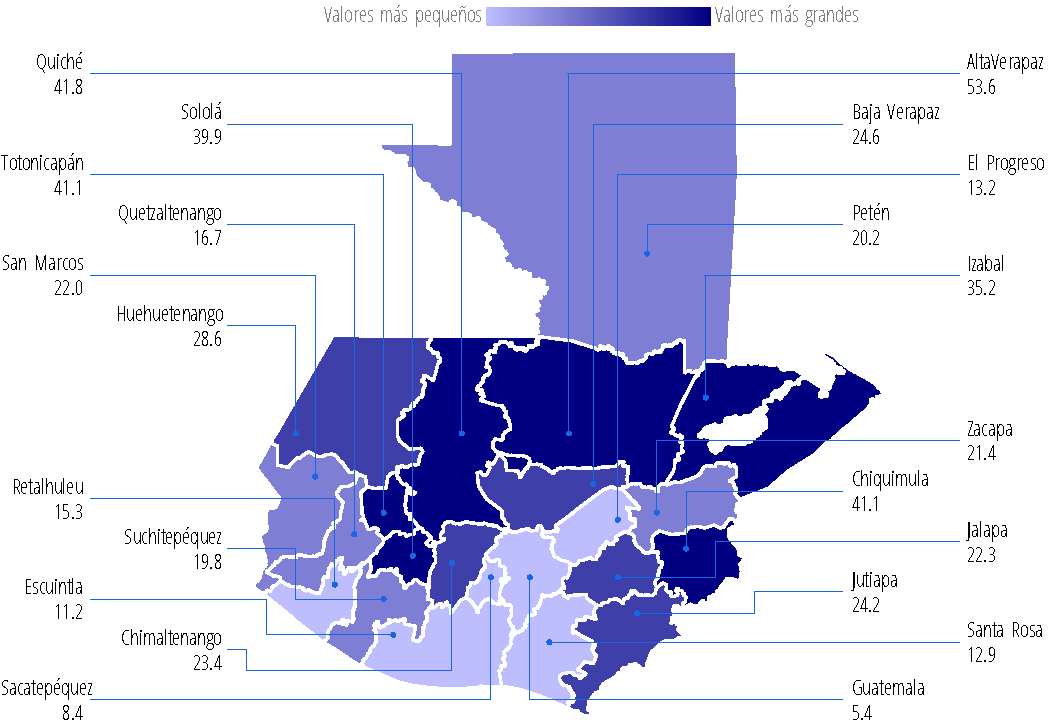
\includegraphics[width=52\cuadri]{graficas/1_12.pdf}}%
{%
 Instituto Nacional de Estadística} %
 
 \cajita{%
Brecha de pobreza total}%
{%
 La brecha de pobreza, muestra la distancia promedio a la que se encuentra la población en pobreza a la línea de pobreza total. Este indicador permite hacer una estimación del monto que sería necesario transferir a los hogares de escasos recursos, para poder salir de la pobreza.   Entre 2000 y 2006, la brecha de pobreza se redujo en 3.2 puntos porcentuales. No obstante, entre 2006 y 2014, la distancia de la población a la línea de pobreza total aumentó 22.0\%, casi el misma distancia observada que para el año 2000.}%
{%
 Brecha de la pobreza total por departamento} %
{%
 Républica de Guatemala, serie histórica por Encovi, en porcentaje} %
{%
 \begin{tikzpicture}[x=1pt,y=1pt]  % Created by tikzDevice version 0.7.0 on 2015-11-27 12:40:15
% !TEX encoding = UTF-8 Unicode
\definecolor[named]{fillColor}{rgb}{1.00,1.00,1.00}
\path[use as bounding box,fill=fillColor,fill opacity=0.00] (0,0) rectangle (289.08,198.74);
\begin{scope}
\path[clip] (  0.00,  0.00) rectangle (289.08,198.74);

\path[] (  0.00,  0.00) rectangle (289.08,198.74);
\end{scope}
\begin{scope}
\path[clip] (  0.00,  0.00) rectangle (289.08,198.74);

\path[] (  1.64, 17.78) rectangle (280.54,191.48);

\path[] (  1.64, 56.04) --
	(280.54, 56.04);

\path[] (  1.64,116.78) --
	(280.54,116.78);

\path[] (  1.64,177.51) --
	(280.54,177.51);

\path[] (  1.64, 25.67) --
	(280.54, 25.67);

\path[] (  1.64, 86.41) --
	(280.54, 86.41);

\path[] (  1.64,147.15) --
	(280.54,147.15);

\path[] ( 53.94, 17.78) --
	( 53.94,191.48);

\path[] (141.09, 17.78) --
	(141.09,191.48);

\path[] (228.25, 17.78) --
	(228.25,191.48);
\definecolor[named]{drawColor}{rgb}{0.00,0.00,1.00}

\path[draw=drawColor,line width= 1.7pt,line join=round] ( 53.94,163.70) --
	(141.09,144.34) --
	(228.25,159.34);
\definecolor[named]{drawColor}{rgb}{0.00,0.00,0.00}

\node[text=drawColor,anchor=base,inner sep=0pt, outer sep=0pt, scale=  1.01] at ( 53.94,167.66) {22.7};

\node[text=drawColor,anchor=base,inner sep=0pt, outer sep=0pt, scale=  1.01] at (141.09,132.47) {19.5};

\node[text=drawColor,anchor=base,inner sep=0pt, outer sep=0pt, scale=  1.01] at (228.25,163.30) {22.0};
\definecolor[named]{fillColor}{rgb}{0.00,0.00,0.00}

\path[draw=drawColor,line width= 0.1pt,line join=round,fill=fillColor] (  1.64, 25.67) -- (280.54, 25.67);

\path[] (  1.64, 17.78) rectangle (280.54,191.48);
\end{scope}
\begin{scope}
\path[clip] (  0.00,  0.00) rectangle (289.08,198.74);

\path[] (  1.64, 17.78) --
	(  1.64,191.48);
\end{scope}
\begin{scope}
\path[clip] (  0.00,  0.00) rectangle (289.08,198.74);

\path[] (  0.00, 25.67) --
	(  1.64, 25.67);

\path[] (  0.00, 86.41) --
	(  1.64, 86.41);

\path[] (  0.00,147.15) --
	(  1.64,147.15);
\end{scope}
\begin{scope}
\path[clip] (  0.00,  0.00) rectangle (289.08,198.74);

\path[] (  1.64, 17.78) --
	(280.54, 17.78);
\end{scope}
\begin{scope}
\path[clip] (  0.00,  0.00) rectangle (289.08,198.74);

\path[] ( 53.94, 13.51) --
	( 53.94, 17.78);

\path[] (141.09, 13.51) --
	(141.09, 17.78);

\path[] (228.25, 13.51) --
	(228.25, 17.78);
\end{scope}
\begin{scope}
\path[clip] (  0.00,  0.00) rectangle (289.08,198.74);
\definecolor[named]{drawColor}{rgb}{0.00,0.00,0.00}

\node[text=drawColor,anchor=base,inner sep=0pt, outer sep=0pt, scale=  1.00] at ( 53.94,  2.85) {2000};

\node[text=drawColor,anchor=base,inner sep=0pt, outer sep=0pt, scale=  1.00] at (141.09,  2.85) {2006};

\node[text=drawColor,anchor=base,inner sep=0pt, outer sep=0pt, scale=  1.00] at (228.25,  2.85) {2014};
\end{scope}
  \end{tikzpicture}}%
{%
 Instituto Nacional de Estadística} %
 
 \cajita{%
Brecha de pobreza extrema}%
{%
 Al combinar el indicador de incidencia y brecha de pobreza, se obtiene la severidad de la pobreza. Para el año 2000, el indicador de severidad de la pobreza era de 11.7\%, entre 2000 y 2006 se observó una reducción en la severidad de la pobreza, tanto por la reducción en el porcentaje de pobreza, como en la distancia promedio a la línea. Para 2014, el índice de severidad aumentó nuevamente, por el aumento de la pobreza, que es menor que la reducción entre 2000 y 2006, y el aumento en la brecha al mismo nivel del observado en el 2000.}%
{%
 Severidad de la pobreza total nacional} %
{%
 Républica de Guatemala, serie histórica por Encovi, en porcentaje} %
{%
 \begin{tikzpicture}[x=1pt,y=1pt]  % Created by tikzDevice version 0.9 on 2015-11-26 22:20:46
% !TEX encoding = UTF-8 Unicode
\definecolor{fillColor}{RGB}{255,255,255}
\path[use as bounding box,fill=fillColor,fill opacity=0.00] (0,0) rectangle (289.08,198.74);
\begin{scope}
\path[clip] (  0.00,  0.00) rectangle (289.08,198.74);

\path[] (  0.00,  0.00) rectangle (289.08,198.74);
\end{scope}
\begin{scope}
\path[clip] (  0.00,  0.00) rectangle (289.08,198.74);

\path[] (  1.64, 17.78) rectangle (280.54,191.48);

\path[] (  1.64, 59.45) --
	(280.54, 59.45);

\path[] (  1.64,114.75) --
	(280.54,114.75);

\path[] (  1.64,170.04) --
	(280.54,170.04);

\path[] (  1.64, 31.81) --
	(280.54, 31.81);

\path[] (  1.64, 87.10) --
	(280.54, 87.10);

\path[] (  1.64,142.39) --
	(280.54,142.39);

\path[] ( 53.94, 17.78) --
	( 53.94,191.48);

\path[] (141.09, 17.78) --
	(141.09,191.48);

\path[] (228.25, 17.78) --
	(228.25,191.48);
\definecolor{drawColor}{RGB}{0,0,255}

\path[draw=drawColor,line width= 1.7pt,line join=round] ( 53.94,183.59) --
	(141.09, 62.11) --
	(228.25,120.91);
\definecolor{drawColor}{RGB}{0,0,0}

\node[text=drawColor,anchor=base,inner sep=0pt, outer sep=0pt, scale=  1.01] at ( 53.94,187.54) {11.7};

\node[text=drawColor,anchor=base,inner sep=0pt, outer sep=0pt, scale=  1.01] at (141.09, 50.24) {9.5};

\node[text=drawColor,anchor=base,inner sep=0pt, outer sep=0pt, scale=  1.01] at (228.25,124.87) {10.6};

\path[draw=drawColor,line width= 0.1pt,line join=round] (  1.64, 25.67) -- (280.54, 25.67);

\path[] (  1.64, 17.78) rectangle (280.54,191.48);
\end{scope}
\begin{scope}
\path[clip] (  0.00,  0.00) rectangle (289.08,198.74);

\path[] (  1.64, 17.78) --
	(  1.64,191.48);
\end{scope}
\begin{scope}
\path[clip] (  0.00,  0.00) rectangle (289.08,198.74);

\path[] (  0.00, 31.81) --
	(  1.64, 31.81);

\path[] (  0.00, 87.10) --
	(  1.64, 87.10);

\path[] (  0.00,142.39) --
	(  1.64,142.39);
\end{scope}
\begin{scope}
\path[clip] (  0.00,  0.00) rectangle (289.08,198.74);

\path[] (  1.64, 17.78) --
	(280.54, 17.78);
\end{scope}
\begin{scope}
\path[clip] (  0.00,  0.00) rectangle (289.08,198.74);

\path[] ( 53.94, 13.51) --
	( 53.94, 17.78);

\path[] (141.09, 13.51) --
	(141.09, 17.78);

\path[] (228.25, 13.51) --
	(228.25, 17.78);
\end{scope}
\begin{scope}
\path[clip] (  0.00,  0.00) rectangle (289.08,198.74);
\definecolor{drawColor}{RGB}{0,0,0}

\node[text=drawColor,anchor=base,inner sep=0pt, outer sep=0pt, scale=  1.00] at ( 53.94,  2.85) {2000};

\node[text=drawColor,anchor=base,inner sep=0pt, outer sep=0pt, scale=  1.00] at (141.09,  2.85) {2006};

\node[text=drawColor,anchor=base,inner sep=0pt, outer sep=0pt, scale=  1.00] at (228.25,  2.85) {2014};
\end{scope}
  \end{tikzpicture}}%
{%
 Instituto Nacional de Estadística} %
 
 \cajota{%
Brecha de la pobreza total en los departamentos}%
{%
 El indicador de severidad de la pobreza, combina el porcentaje de pobreza y la distancia promedio a la línea de pobreza, por lo que al momento de hacer comparaciones entre departamentos, permite identificar a los que se encuentran en peores condiciones.  Se puede observar que el departamento de Alta Verapaz presenta las condiciones de pobreza más severas, seguido del departamento de Chiquimula, Totonicapán y Sololá. Mientras que en Guatemala, Sacatepéquez y Escuintla, el índice de severidad es menor, que coincide con menores porcentajes de incidencia y brecha de la pobreza. }%
{%
 Brecha de la pobreza total por departamento} %
{%
 Por departamento, Encovi 2014, en porcentaje} %
{%
 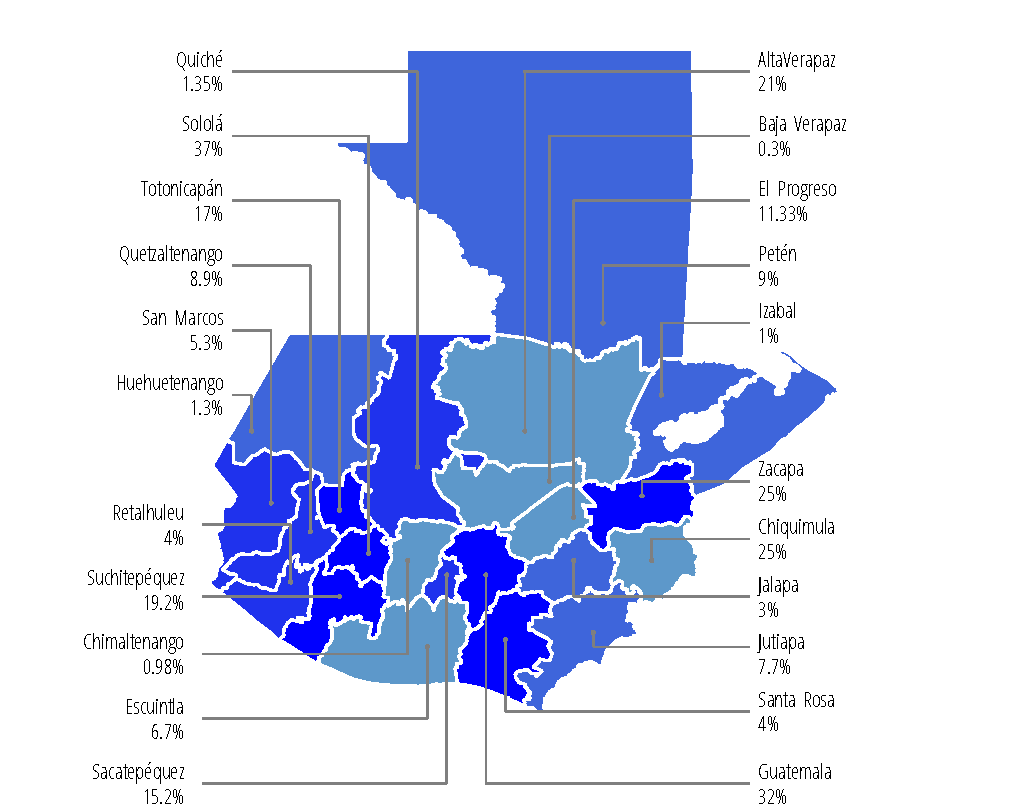
\includegraphics[width=52\cuadri]{graficas/1_15.pdf}}%
{%
 Instituto Nacional de Estadística} %
 
 \cajita{%
Severidad de la pobreza}%
{%
 Al combinar el indicador de incidencia y brecha de pobreza, se obtiene la severidad de la pobreza. Para el año 2000, el indicador de severidad de la pobreza era de 11.7\%, entre 2000 y 2006 se observó una reducción en la severidad de la pobreza, tanto por la reducción en el porcentaje de pobreza, como en la distancia promedio a la línea. Para 2014, el índice de severidad aumentó nuevamente, por el aumento de la pobreza, que es menor que la reducción entre 2000 y 2006, y el aumento en la brecha al mismo nivel del observado en el 2000.}%
{%
 Severidad de la pobreza total nacional} %
{%
 Républica de Guatemala, serie histórica por Encovi, en porcentaje} %
{%
 \begin{tikzpicture}[x=1pt,y=1pt]  % Created by tikzDevice version 0.7.0 on 2015-11-27 11:12:45
% !TEX encoding = UTF-8 Unicode
\definecolor[named]{fillColor}{rgb}{1.00,1.00,1.00}
\path[use as bounding box,fill=fillColor,fill opacity=0.00] (0,0) rectangle (289.08,198.74);
\begin{scope}
\path[clip] (  0.00,  0.00) rectangle (289.08,198.74);

\path[] (  0.00,  0.00) rectangle (289.08,198.74);
\end{scope}
\begin{scope}
\path[clip] (  0.00,  0.00) rectangle (289.08,198.74);

\path[] (  1.64, 17.78) rectangle (280.54,191.48);

\path[] (  1.64, 59.45) --
	(280.54, 59.45);

\path[] (  1.64,114.75) --
	(280.54,114.75);

\path[] (  1.64,170.04) --
	(280.54,170.04);

\path[] (  1.64, 31.81) --
	(280.54, 31.81);

\path[] (  1.64, 87.10) --
	(280.54, 87.10);

\path[] (  1.64,142.39) --
	(280.54,142.39);

\path[] ( 53.94, 17.78) --
	( 53.94,191.48);

\path[] (141.09, 17.78) --
	(141.09,191.48);

\path[] (228.25, 17.78) --
	(228.25,191.48);
\definecolor[named]{drawColor}{rgb}{0.00,0.00,1.00}

\path[draw=drawColor,line width= 1.7pt,line join=round] ( 53.94,183.59) --
	(141.09, 62.11) --
	(228.25,120.91);
\definecolor[named]{drawColor}{rgb}{0.00,0.00,0.00}

\node[text=drawColor,anchor=base,inner sep=0pt, outer sep=0pt, scale=  1.01] at ( 53.94,187.54) {11.7};

\node[text=drawColor,anchor=base,inner sep=0pt, outer sep=0pt, scale=  1.01] at (141.09, 50.24) {9.5};

\node[text=drawColor,anchor=base,inner sep=0pt, outer sep=0pt, scale=  1.01] at (228.25,124.87) {10.6};
\definecolor[named]{fillColor}{rgb}{0.00,0.00,0.00}

\path[draw=drawColor,line width= 0.1pt,line join=round,fill=fillColor] (  1.64, 25.67) -- (280.54, 25.67);

\path[] (  1.64, 17.78) rectangle (280.54,191.48);
\end{scope}
\begin{scope}
\path[clip] (  0.00,  0.00) rectangle (289.08,198.74);

\path[] (  1.64, 17.78) --
	(  1.64,191.48);
\end{scope}
\begin{scope}
\path[clip] (  0.00,  0.00) rectangle (289.08,198.74);

\path[] (  0.00, 31.81) --
	(  1.64, 31.81);

\path[] (  0.00, 87.10) --
	(  1.64, 87.10);

\path[] (  0.00,142.39) --
	(  1.64,142.39);
\end{scope}
\begin{scope}
\path[clip] (  0.00,  0.00) rectangle (289.08,198.74);

\path[] (  1.64, 17.78) --
	(280.54, 17.78);
\end{scope}
\begin{scope}
\path[clip] (  0.00,  0.00) rectangle (289.08,198.74);

\path[] ( 53.94, 13.51) --
	( 53.94, 17.78);

\path[] (141.09, 13.51) --
	(141.09, 17.78);

\path[] (228.25, 13.51) --
	(228.25, 17.78);
\end{scope}
\begin{scope}
\path[clip] (  0.00,  0.00) rectangle (289.08,198.74);
\definecolor[named]{drawColor}{rgb}{0.00,0.00,0.00}

\node[text=drawColor,anchor=base,inner sep=0pt, outer sep=0pt, scale=  1.00] at ( 53.94,  2.85) {2000};

\node[text=drawColor,anchor=base,inner sep=0pt, outer sep=0pt, scale=  1.00] at (141.09,  2.85) {2006};

\node[text=drawColor,anchor=base,inner sep=0pt, outer sep=0pt, scale=  1.00] at (228.25,  2.85) {2014};
\end{scope}
  \end{tikzpicture}}%
{%
 Instituto Nacional de Estadística} %
 
 \cajota{%
Severidad de la pobreza total en los departamentos}%
{%
   Se puede observar que el departamento de Alta Verapaz presenta las condiciones de pobreza más severas, seguido del departamento de Chiquimula, Totonicapán y Sololá. Mientras que en Guatemala, Sacatepéquez y Escuintla, el índice de severidad es menor, que coincide con menores porcentajes de incidencia y brecha de la pobreza. }%
{%
 Severidad de la pobreza total por departamento} %
{%
 Por departamento, Encovi 2014, en porcentaje} %
{%
 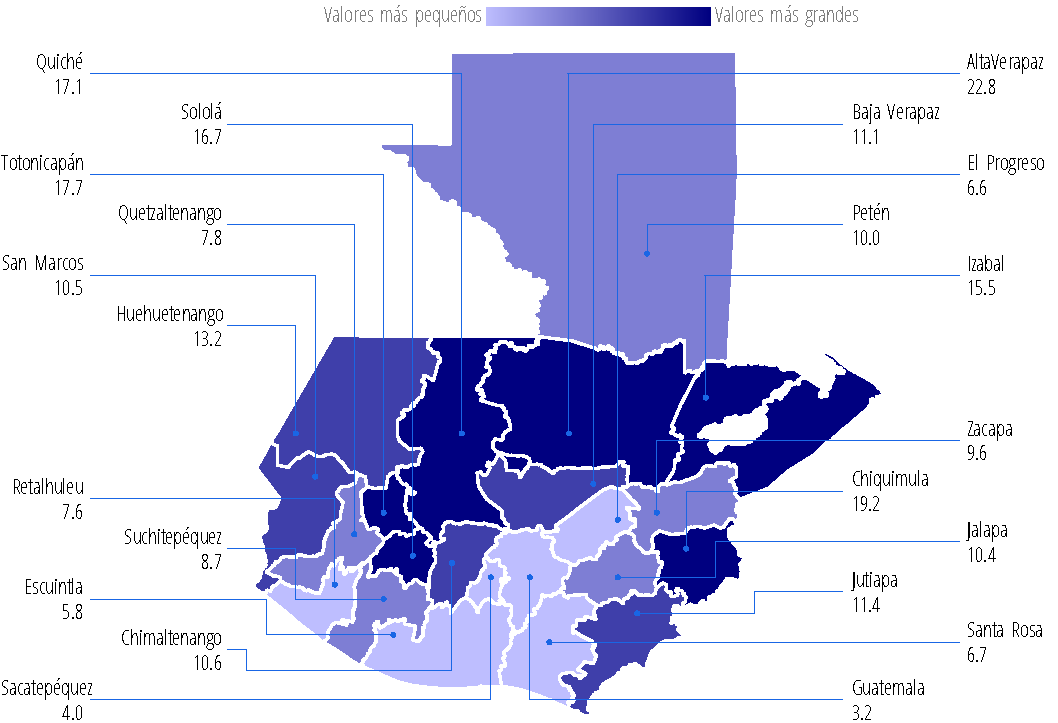
\includegraphics[width=52\cuadri]{graficas/1_17.pdf}}%
{%
 Instituto Nacional de Estadística} %
 
 \cajita{%
Pobreza en niños y adolescentes}%
{%
 Para 2014, el 68.2\% de los menores de 18 años\footnote{Según el artículo 8 del Código Civil de Guatemala: \textit{"Son mayores de edad los que han cumplido 18 años."}} habitaban en hogares pobres. Al desagregar por rangos de edad, se obtiene que el 70.2\% de los niños menores de 10 años se encontraban en pobreza. Mientas que para los niños-adolescentes entre 10 y 17 años, la pobreza era de 65.9\%.}%
{%
 Proporción de la población menor de 20 años que habitan en hogares en pobreza} %
{%
 República de Guatemala, Encovi 2014 en porcentaje} %
{%
 \begin{tikzpicture}[x=1pt,y=1pt]  % Created by tikzDevice version 0.7.0 on 2015-11-27 12:55:06
% !TEX encoding = UTF-8 Unicode
\definecolor[named]{fillColor}{rgb}{1.00,1.00,1.00}
\path[use as bounding box,fill=fillColor,fill opacity=0.00] (0,0) rectangle (289.08,198.74);
\begin{scope}
\path[clip] (  0.00,  0.00) rectangle (289.08,198.74);

\path[] (  0.00,  0.00) rectangle (289.08,198.74);
\end{scope}
\begin{scope}
\path[clip] (  0.00,  0.00) rectangle (289.08,198.74);

\path[] (  8.54, 16.35) rectangle (289.08,181.67);

\path[] ( 61.14, 16.35) --
	( 61.14,181.67);

\path[] (148.81, 16.35) --
	(148.81,181.67);

\path[] (236.48, 16.35) --
	(236.48,181.67);
\definecolor[named]{drawColor}{rgb}{0.00,0.00,1.00}
\definecolor[named]{fillColor}{rgb}{0.00,0.00,1.00}

\path[draw=drawColor,line width= 0.6pt,line join=round,fill=fillColor] ( 43.60, 23.87) rectangle ( 78.67,169.87);

\path[draw=drawColor,line width= 0.6pt,line join=round,fill=fillColor] (131.27, 23.87) rectangle (166.34,174.16);

\path[draw=drawColor,line width= 0.6pt,line join=round,fill=fillColor] (218.94, 23.87) rectangle (254.01,164.95);
\definecolor[named]{drawColor}{rgb}{0.00,0.00,0.00}
\definecolor[named]{fillColor}{rgb}{0.00,0.00,0.00}

\path[draw=drawColor,line width= 0.1pt,line join=round,fill=fillColor] (  8.54, 23.87) -- (289.08, 23.87);

\node[text=drawColor,anchor=base,inner sep=0pt, outer sep=0pt, scale=  1.01] at ( 61.14,173.83) {68.2};

\node[text=drawColor,anchor=base,inner sep=0pt, outer sep=0pt, scale=  1.01] at (148.81,178.11) {70.2};

\node[text=drawColor,anchor=base,inner sep=0pt, outer sep=0pt, scale=  1.01] at (236.48,168.91) {65.9};

\path[] (  8.54, 16.35) rectangle (289.08,181.67);
\end{scope}
\begin{scope}
\path[clip] (  0.00,  0.00) rectangle (289.08,198.74);

\path[] (  8.54, 16.35) --
	(  8.54,181.67);
\end{scope}
\begin{scope}
\path[clip] (  0.00,  0.00) rectangle (289.08,198.74);

\path[] (  8.54, 16.35) --
	(289.08, 16.35);
\end{scope}
\begin{scope}
\path[clip] (  0.00,  0.00) rectangle (289.08,198.74);

\path[] ( 61.14, 12.08) --
	( 61.14, 16.35);

\path[] (148.81, 12.08) --
	(148.81, 16.35);

\path[] (236.48, 12.08) --
	(236.48, 16.35);
\end{scope}
\begin{scope}
\path[clip] (  0.00,  0.00) rectangle (289.08,198.74);
\definecolor[named]{drawColor}{rgb}{0.00,0.00,0.00}

\node[text=drawColor,anchor=base,inner sep=0pt, outer sep=0pt, scale=  1.00] at ( 61.14,  6.04) {De 0 a 17};

\node[text=drawColor,anchor=base,inner sep=0pt, outer sep=0pt, scale=  1.00] at (148.81,  6.04) {De 0 a 9};

\node[text=drawColor,anchor=base,inner sep=0pt, outer sep=0pt, scale=  1.00] at (236.48,  6.04) {De 10 a 17};
\end{scope}
  \end{tikzpicture}}%
{%
 Instituto Nacional de Estadística} %
  
\INEchaptercarta{Pobreza}{La metodología de líneas de pobreza absoluta consiste en fijar el costo mínimo necesario para cubrir una canasta que permita satisfacer las necesidades alimentarias y no alimentarias. Se considera pobre a la proporción de población que no logra acceder a este umbral. Con estos resultados se clasifica a la población en pobreza extrema, a aquellos que no alcanzan a cubrir el costo del consumo mínimo de alimentos, y pobreza total, a los que alcanzan a cubrir el costo del consumo mínimo de alimentos, pero no así, el costo mínimo adicional para otros bienes y servicios básicos. 
	
A continuación se presentan los resultados de pobreza extrema y total de 2000, 2006 y 2014, que son los indicadores estadísticamente comparables debido a que fueron calculados siguiendo la metodología propuesta por el Banco Mundial.
	}

 \cajita{%
Línea de pobreza total }%
{%
  Para el año 2000, el valor de la línea de pobreza total\footnote{La línea de pobreza total incluye, además del costo alimenticio, un monto adicional que corresponde al porcentaje de consumo no alimenticio de las personas, cuyo consumo de alimentos se encuentra alrededor de la línea de pobreza extrema.} era de Q 4,319\footnote{ Este valor ajustado a precios de 2014  equivale a 10,000  quetzales. }.
 
  Se puede observar que para 2014, el costo de alimentación más bienes y servicios, aumentó a Q 10,218 lo que equivale a un incremento del 137\% .}%
{%
 Líneas de pobreza total nacional} %
{%
 Républica de Guatemala, Encovi 2000, 2006 y 2014, en quetzales de cada año} %
{%
 \begin{tikzpicture}[x=1pt,y=1pt]  % Created by tikzDevice version 0.7.0 on 2015-11-27 11:12:31
% !TEX encoding = UTF-8 Unicode
\definecolor[named]{fillColor}{rgb}{1.00,1.00,1.00}
\path[use as bounding box,fill=fillColor,fill opacity=0.00] (0,0) rectangle (289.08,198.74);
\begin{scope}
\path[clip] (  0.00,  0.00) rectangle (289.08,198.74);

\path[] (  0.00,  0.00) rectangle (289.08,198.74);
\end{scope}
\begin{scope}
\path[clip] (  0.00,  0.00) rectangle (289.08,198.74);

\path[] ( 14.78, 17.78) rectangle (280.54,191.48);

\path[] ( 14.78, 34.98) --
	(280.54, 34.98);

\path[] ( 14.78, 76.15) --
	(280.54, 76.15);

\path[] ( 14.78,117.33) --
	(280.54,117.33);

\path[] ( 14.78,158.51) --
	(280.54,158.51);

\path[] ( 14.78, 55.57) --
	(280.54, 55.57);

\path[] ( 14.78, 96.74) --
	(280.54, 96.74);

\path[] ( 14.78,137.92) --
	(280.54,137.92);

\path[] ( 14.78,179.10) --
	(280.54,179.10);

\path[] ( 64.61, 17.78) --
	( 64.61,191.48);

\path[] (147.66, 17.78) --
	(147.66,191.48);

\path[] (230.71, 17.78) --
	(230.71,191.48);
\definecolor[named]{drawColor}{rgb}{0.00,0.00,1.00}

\path[draw=drawColor,line width= 1.7pt,line join=round] ( 64.61, 62.11) --
	(147.66,108.56) --
	(230.71,183.59);
\definecolor[named]{drawColor}{rgb}{0.00,0.00,0.00}

\node[text=drawColor,anchor=base,inner sep=0pt, outer sep=0pt, scale=  1.01] at ( 64.61, 50.24) {4,318};

\node[text=drawColor,anchor=base east,inner sep=0pt, outer sep=0pt, scale=  1.01] at (143.66,108.56) {6,574};

\node[text=drawColor,anchor=base,inner sep=0pt, outer sep=0pt, scale=  1.01] at (230.71,187.54) {10,218};
\definecolor[named]{fillColor}{rgb}{0.00,0.00,0.00}

\path[draw=drawColor,line width= 0.1pt,line join=round,fill=fillColor] ( 14.78, 25.67) -- (280.54, 25.67);

\path[] ( 14.78, 17.78) rectangle (280.54,191.48);
\end{scope}
\begin{scope}
\path[clip] (  0.00,  0.00) rectangle (289.08,198.74);

\path[] ( 14.78, 17.78) --
	( 14.78,191.48);
\end{scope}
\begin{scope}
\path[clip] (  0.00,  0.00) rectangle (289.08,198.74);
\definecolor[named]{drawColor}{rgb}{1.00,1.00,1.00}

\node[text=drawColor,text opacity=0.00,anchor=base east,inner sep=0pt, outer sep=0pt, scale=  1.00] at (  7.67, 51.66) {4000};

\node[text=drawColor,text opacity=0.00,anchor=base east,inner sep=0pt, outer sep=0pt, scale=  1.00] at (  7.67, 92.84) {6000};

\node[text=drawColor,text opacity=0.00,anchor=base east,inner sep=0pt, outer sep=0pt, scale=  1.00] at (  7.67,134.01) {8000};

\node[text=drawColor,text opacity=0.00,anchor=base east,inner sep=0pt, outer sep=0pt, scale=  1.00] at (  7.67,175.19) {10000};
\end{scope}
\begin{scope}
\path[clip] (  0.00,  0.00) rectangle (289.08,198.74);

\path[] ( 10.51, 55.57) --
	( 14.78, 55.57);

\path[] ( 10.51, 96.74) --
	( 14.78, 96.74);

\path[] ( 10.51,137.92) --
	( 14.78,137.92);

\path[] ( 10.51,179.10) --
	( 14.78,179.10);
\end{scope}
\begin{scope}
\path[clip] (  0.00,  0.00) rectangle (289.08,198.74);

\path[] ( 14.78, 17.78) --
	(280.54, 17.78);
\end{scope}
\begin{scope}
\path[clip] (  0.00,  0.00) rectangle (289.08,198.74);

\path[] ( 64.61, 13.51) --
	( 64.61, 17.78);

\path[] (147.66, 13.51) --
	(147.66, 17.78);

\path[] (230.71, 13.51) --
	(230.71, 17.78);
\end{scope}
\begin{scope}
\path[clip] (  0.00,  0.00) rectangle (289.08,198.74);
\definecolor[named]{drawColor}{rgb}{0.00,0.00,0.00}

\node[text=drawColor,anchor=base,inner sep=0pt, outer sep=0pt, scale=  1.00] at ( 64.61,  2.85) {2000};

\node[text=drawColor,anchor=base,inner sep=0pt, outer sep=0pt, scale=  1.00] at (147.66,  2.85) {2006};

\node[text=drawColor,anchor=base,inner sep=0pt, outer sep=0pt, scale=  1.00] at (230.71,  2.85) {2014};
\end{scope}
  \end{tikzpicture}}%
{%
 Instituto Nacional de Estadística} %
 
 \cajita{%
Pobreza total}%
{%
 Trae fórmula Nota: indicador FGT (Foster, Greer y Thorbecke) Para 2014, el 59.3\% de la población se encontraba por debajo de la línea de pobreza total, es decir, más de la mitad de la población tenía un consumo por debajo de Q10,218 al año. Se puede observar en la gráfica  que entre 2000 y 2014, la pobreza total aumentó en 2.9 puntos porcentuales, pasando de 56.4\% en 2000 a 59.3\% en 2014.}%
{%
 Incidencia de pobreza total nacional} %
{%
 Républica de Guatemala, serie histórica por Encovi, en porcentaje} %
{%
 \begin{tikzpicture}[x=1pt,y=1pt]  % Created by tikzDevice version 0.7.0 on 2015-11-27 11:12:32
% !TEX encoding = UTF-8 Unicode
\definecolor[named]{fillColor}{rgb}{1.00,1.00,1.00}
\path[use as bounding box,fill=fillColor,fill opacity=0.00] (0,0) rectangle (289.08,198.74);
\begin{scope}
\path[clip] (  0.00,  0.00) rectangle (289.08,198.74);

\path[] (  0.00,  0.00) rectangle (289.08,198.74);
\end{scope}
\begin{scope}
\path[clip] (  0.00,  0.00) rectangle (289.08,198.74);

\path[] (  1.64, 17.78) rectangle (280.54,191.48);

\path[] (  1.64, 37.36) --
	(280.54, 37.36);

\path[] (  1.64, 82.20) --
	(280.54, 82.20);

\path[] (  1.64,127.03) --
	(280.54,127.03);

\path[] (  1.64,171.86) --
	(280.54,171.86);

\path[] (  1.64, 59.78) --
	(280.54, 59.78);

\path[] (  1.64,104.61) --
	(280.54,104.61);

\path[] (  1.64,149.44) --
	(280.54,149.44);

\path[] ( 53.94, 17.78) --
	( 53.94,191.48);

\path[] (141.09, 17.78) --
	(141.09,191.48);

\path[] (228.25, 17.78) --
	(228.25,191.48);
\definecolor[named]{drawColor}{rgb}{0.00,0.00,1.00}

\path[draw=drawColor,line width= 1.7pt,line join=round] ( 53.94,140.63) --
	(141.09, 62.11) --
	(228.25,183.59);
\definecolor[named]{drawColor}{rgb}{0.00,0.00,0.00}

\node[text=drawColor,anchor=base,inner sep=0pt, outer sep=0pt, scale=  1.01] at ( 53.94,144.58) {56.4};

\node[text=drawColor,anchor=base,inner sep=0pt, outer sep=0pt, scale=  1.01] at (141.09, 50.24) {51.2};

\node[text=drawColor,anchor=base,inner sep=0pt, outer sep=0pt, scale=  1.01] at (228.25,187.54) {59.3};
\definecolor[named]{fillColor}{rgb}{0.00,0.00,0.00}

\path[draw=drawColor,line width= 0.1pt,line join=round,fill=fillColor] (  1.64, 25.67) -- (280.54, 25.67);

\path[] (  1.64, 17.78) rectangle (280.54,191.48);
\end{scope}
\begin{scope}
\path[clip] (  0.00,  0.00) rectangle (289.08,198.74);

\path[] (  1.64, 17.78) --
	(  1.64,191.48);
\end{scope}
\begin{scope}
\path[clip] (  0.00,  0.00) rectangle (289.08,198.74);

\path[] (  0.00, 59.78) --
	(  1.64, 59.78);

\path[] (  0.00,104.61) --
	(  1.64,104.61);

\path[] (  0.00,149.44) --
	(  1.64,149.44);
\end{scope}
\begin{scope}
\path[clip] (  0.00,  0.00) rectangle (289.08,198.74);

\path[] (  1.64, 17.78) --
	(280.54, 17.78);
\end{scope}
\begin{scope}
\path[clip] (  0.00,  0.00) rectangle (289.08,198.74);

\path[] ( 53.94, 13.51) --
	( 53.94, 17.78);

\path[] (141.09, 13.51) --
	(141.09, 17.78);

\path[] (228.25, 13.51) --
	(228.25, 17.78);
\end{scope}
\begin{scope}
\path[clip] (  0.00,  0.00) rectangle (289.08,198.74);
\definecolor[named]{drawColor}{rgb}{0.00,0.00,0.00}

\node[text=drawColor,anchor=base,inner sep=0pt, outer sep=0pt, scale=  1.00] at ( 53.94,  2.85) {2000};

\node[text=drawColor,anchor=base,inner sep=0pt, outer sep=0pt, scale=  1.00] at (141.09,  2.85) {2006};

\node[text=drawColor,anchor=base,inner sep=0pt, outer sep=0pt, scale=  1.00] at (228.25,  2.85) {2014};
\end{scope}
  \end{tikzpicture}}%
{%
 Instituto Nacional de Estadística} %
 
 \cajita{%
Pobreza total por etnicidad}%
{%
 Para 2014, casi cuatro de cada cinco personas indígenas se encontraba en pobreza. Al comparar los niveles de pobreza con la población no indígena, se obtiene que la pobreza en la población indígena era 1.7 veces mayor que en la población no indígena. Se puede observar que entre 2000 y 2014, hubo un aumento de la pobreza para ambos grupos, aunque el aumento fue mayor en la población no indígena que en la población indígena, 4.7 y 1.9 puntos porcentuales, respectivamente.}%
{%
 Incidencia de pobreza total por etnicidad} %
{%
 Républica de Guatemala, serie histórica por Encovi, en porcentaje} %
{%
 \begin{tikzpicture}[x=1pt,y=1pt]  % Created by tikzDevice version 0.9 on 2015-12-01 14:57:19
% !TEX encoding = UTF-8 Unicode
\definecolor{fillColor}{RGB}{255,255,255}
\path[use as bounding box,fill=fillColor,fill opacity=0.00] (0,0) rectangle (289.08,198.74);
\begin{scope}
\path[clip] (  0.00,  0.00) rectangle (289.08,198.74);

\path[] (  0.00,  0.00) rectangle (289.08,198.74);
\end{scope}
\begin{scope}
\path[clip] (  0.00,  0.00) rectangle (289.08,198.74);

\path[] (  7.11, 20.62) rectangle (289.08,172.42);

\path[] ( 59.98, 20.62) --
	( 59.98,172.42);

\path[] (148.10, 20.62) --
	(148.10,172.42);

\path[] (236.21, 20.62) --
	(236.21,172.42);
\definecolor{drawColor}{RGB}{0,0,255}
\definecolor{fillColor}{RGB}{0,0,255}

\path[draw=drawColor,line width= 0.6pt,line join=round,fill=fillColor] ( 26.94, 20.62) rectangle ( 53.37,168.70);
\definecolor{drawColor}{RGB}{157,187,255}
\definecolor{fillColor}{RGB}{157,187,255}

\path[draw=drawColor,line width= 0.6pt,line join=round,fill=fillColor] ( 66.59, 20.62) rectangle ( 93.02,100.90);
\definecolor{drawColor}{RGB}{0,0,255}
\definecolor{fillColor}{RGB}{0,0,255}

\path[draw=drawColor,line width= 0.6pt,line join=round,fill=fillColor] (115.05, 20.62) rectangle (141.49,164.31);
\definecolor{drawColor}{RGB}{157,187,255}
\definecolor{fillColor}{RGB}{157,187,255}

\path[draw=drawColor,line width= 0.6pt,line join=round,fill=fillColor] (154.71, 20.62) rectangle (181.14, 90.23);
\definecolor{drawColor}{RGB}{0,0,255}
\definecolor{fillColor}{RGB}{0,0,255}

\path[draw=drawColor,line width= 0.6pt,line join=round,fill=fillColor] (203.17, 20.62) rectangle (229.60,172.42);
\definecolor{drawColor}{RGB}{157,187,255}
\definecolor{fillColor}{RGB}{157,187,255}

\path[draw=drawColor,line width= 0.6pt,line join=round,fill=fillColor] (242.82, 20.62) rectangle (269.25,109.86);
\definecolor{drawColor}{RGB}{0,0,0}

\path[draw=drawColor,line width= 0.6pt,line join=round] (  7.11, 20.62) -- (289.08, 20.62);

\node[text=drawColor,anchor=base,inner sep=0pt, outer sep=0pt, scale=  0.82] at ( 40.16,171.92) {77.3};

\node[text=drawColor,anchor=base,inner sep=0pt, outer sep=0pt, scale=  0.82] at ( 79.81,104.13) {41.9};

\node[text=drawColor,anchor=base,inner sep=0pt, outer sep=0pt, scale=  0.82] at (128.27,167.53) {75.0};

\node[text=drawColor,anchor=base,inner sep=0pt, outer sep=0pt, scale=  0.82] at (167.92, 93.45) {36.3};

\node[text=drawColor,anchor=base,inner sep=0pt, outer sep=0pt, scale=  0.82] at (216.39,175.65) {79.2};

\node[text=drawColor,anchor=base,inner sep=0pt, outer sep=0pt, scale=  0.82] at (256.04,113.08) {46.6};

\path[] (  7.11, 20.62) rectangle (289.08,172.42);
\end{scope}
\begin{scope}
\path[clip] (  0.00,  0.00) rectangle (289.08,198.74);

\path[] (  7.11, 20.62) --
	(  7.11,172.42);
\end{scope}
\begin{scope}
\path[clip] (  0.00,  0.00) rectangle (289.08,198.74);

\path[] (  7.11, 20.62) --
	(289.08, 20.62);
\end{scope}
\begin{scope}
\path[clip] (  0.00,  0.00) rectangle (289.08,198.74);

\path[] ( 59.98, 16.35) --
	( 59.98, 20.62);

\path[] (148.10, 16.35) --
	(148.10, 20.62);

\path[] (236.21, 16.35) --
	(236.21, 20.62);
\end{scope}
\begin{scope}
\path[clip] (  0.00,  0.00) rectangle (289.08,198.74);
\definecolor{drawColor}{RGB}{0,0,0}

\node[text=drawColor,anchor=base,inner sep=0pt, outer sep=0pt, scale=  1.00] at ( 59.98,  5.69) {2000};

\node[text=drawColor,anchor=base,inner sep=0pt, outer sep=0pt, scale=  1.00] at (148.10,  5.69) {2006};

\node[text=drawColor,anchor=base,inner sep=0pt, outer sep=0pt, scale=  1.00] at (236.21,  5.69) {2014};
\end{scope}
\begin{scope}
\path[clip] (  0.00,  0.00) rectangle (289.08,198.74);
\coordinate (apoyo) at (55.19,188.79);
\coordinate (longitudFicticia) at (7.11,9.95);
\coordinate (longitud) at (7.11,7.11);
\coordinate (desX) at (133.24,0);
\coordinate (desY) at (0,1.42);
\definecolor[named]{ct1}{HTML}{
0000FF
}
\definecolor[named]{ct2}{HTML}{
9DBBFF
}
\definecolor[named]{ctb1}{HTML}{
0000FF
}
\definecolor[named]{ctb2}{HTML}{
9DBBFF
}
\path [fill=none] (apoyo) rectangle ($(apoyo)+(longitudFicticia)$)
node [xshift=0.3cm,inner sep=0pt, outer sep=0pt,midway,right,scale = 0.9]{Indígena};
\draw [color = ctb1,fill=ct1] ( $(apoyo)  + (desY) $) rectangle ($(apoyo)+ (desY) +(longitud)$);
\path [fill=none] ($(apoyo)+(desX)$) rectangle ($(apoyo)+(desX)+(longitudFicticia)$)
node [xshift=0.3cm,inner sep=0pt, outer sep=0pt,midway,right,scale = 0.9]{No indígena};
\draw [color = ctb2 ,fill=ct2] ( $(apoyo)  + (desY) + (desX) $) rectangle ($(apoyo)+ (desY)+ (desX) +(longitud)$);
\end{scope}
  \end{tikzpicture}}%
{%
 Instituto Nacional de Estadística} %
 
 \cajita{%
Pobreza total por área de residencia}%
{%
 Según las estimaciones de pobreza, entre 2000 y 2014 hubo un aumento de la pobreza, tanto en el área urbana como en el área rural, siendo superior la pobreza en el área rural.  En la gráfica se advierte que la brecha entre la pobreza en el área urbana y el área rural se ha ido reduciendo en este período, ya que para el año 2000 la pobreza en el área rural era 2.7 veces mayor que en el área urbana, y para 2014 se redujo a 1.8. }%
{%
 Incidencia de pobreza total por área de residencia} %
{%
 Républica de Guatemala, serie histórica por Encovi, en porcentaje} %
{%
 \begin{tikzpicture}[x=1pt,y=1pt]  % Created by tikzDevice version 0.9 on 2015-11-26 21:53:05
% !TEX encoding = UTF-8 Unicode
\definecolor{fillColor}{RGB}{255,255,255}
\path[use as bounding box,fill=fillColor,fill opacity=0.00] (0,0) rectangle (289.08,198.74);
\begin{scope}
\path[clip] (  0.00,  0.00) rectangle (289.08,198.74);

\path[] (  0.00,  0.00) rectangle (289.08,198.74);
\end{scope}
\begin{scope}
\path[clip] (  0.00,  0.00) rectangle (289.08,198.74);

\path[] (  7.11, 20.62) rectangle (289.08,172.42);

\path[] ( 47.39, 20.62) --
	( 47.39,172.42);

\path[] (114.53, 20.62) --
	(114.53,172.42);

\path[] (181.66, 20.62) --
	(181.66,172.42);

\path[] (248.80, 20.62) --
	(248.80,172.42);
\definecolor{drawColor}{RGB}{0,0,255}
\definecolor{fillColor}{RGB}{0,0,255}

\path[draw=drawColor,line width= 0.6pt,line join=round,fill=fillColor] ( 18.86, 20.62) rectangle ( 45.72,172.42);
\definecolor{drawColor}{RGB}{157,187,255}
\definecolor{fillColor}{RGB}{157,187,255}

\path[draw=drawColor,line width= 0.6pt,line join=round,fill=fillColor] ( 49.07, 20.62) rectangle ( 75.93,102.92);
\definecolor{drawColor}{RGB}{0,0,255}
\definecolor{fillColor}{RGB}{0,0,255}

\path[draw=drawColor,line width= 0.6pt,line join=round,fill=fillColor] ( 86.00, 20.62) rectangle (112.85,167.92);
\definecolor{drawColor}{RGB}{157,187,255}
\definecolor{fillColor}{RGB}{157,187,255}

\path[draw=drawColor,line width= 0.6pt,line join=round,fill=fillColor] (116.21, 20.62) rectangle (143.06, 91.98);
\definecolor{drawColor}{RGB}{0,0,255}
\definecolor{fillColor}{RGB}{0,0,255}

\path[draw=drawColor,line width= 0.6pt,line join=round,fill=fillColor] (153.13, 20.62) rectangle (179.99,164.83);
\definecolor{drawColor}{RGB}{157,187,255}
\definecolor{fillColor}{RGB}{157,187,255}

\path[draw=drawColor,line width= 0.6pt,line join=round,fill=fillColor] (183.34, 20.62) rectangle (210.20,100.35);
\definecolor{drawColor}{RGB}{0,0,255}
\definecolor{fillColor}{RGB}{0,0,255}

\path[draw=drawColor,line width= 0.6pt,line join=round,fill=fillColor] (220.27, 20.62) rectangle (247.12, 20.62);
\definecolor{drawColor}{RGB}{157,187,255}
\definecolor{fillColor}{RGB}{157,187,255}

\path[draw=drawColor,line width= 0.6pt,line join=round,fill=fillColor] (250.48, 20.62) rectangle (277.33, 20.62);
\definecolor{drawColor}{RGB}{0,0,0}

\path[draw=drawColor,line width= 0.6pt,line join=round] (  7.11, 20.62) -- (289.08, 20.62);

\node[text=drawColor,anchor=base,inner sep=0pt, outer sep=0pt, scale=  0.82] at ( 32.29,175.65) {77.3};

\node[text=drawColor,anchor=base,inner sep=0pt, outer sep=0pt, scale=  0.82] at ( 62.50,106.15) {41.9};

\node[text=drawColor,anchor=base,inner sep=0pt, outer sep=0pt, scale=  0.82] at ( 99.42,171.15) {75.0};

\node[text=drawColor,anchor=base,inner sep=0pt, outer sep=0pt, scale=  0.82] at (129.63, 95.20) {36.3};

\node[text=drawColor,anchor=base,inner sep=0pt, outer sep=0pt, scale=  0.82] at (166.56,168.05) {73.4};

\node[text=drawColor,anchor=base,inner sep=0pt, outer sep=0pt, scale=  0.82] at (196.77,103.57) {40.6};

\node[text=drawColor,anchor=base,inner sep=0pt, outer sep=0pt, scale=  0.82] at (233.69, 23.84) {0.0};

\node[text=drawColor,anchor=base,inner sep=0pt, outer sep=0pt, scale=  0.82] at (263.90, 23.84) {0.0};

\path[] (  7.11, 20.62) rectangle (289.08,172.42);
\end{scope}
\begin{scope}
\path[clip] (  0.00,  0.00) rectangle (289.08,198.74);

\path[] (  7.11, 20.62) --
	(  7.11,172.42);
\end{scope}
\begin{scope}
\path[clip] (  0.00,  0.00) rectangle (289.08,198.74);

\path[] (  7.11, 20.62) --
	(289.08, 20.62);
\end{scope}
\begin{scope}
\path[clip] (  0.00,  0.00) rectangle (289.08,198.74);

\path[] ( 47.39, 16.35) --
	( 47.39, 20.62);

\path[] (114.53, 16.35) --
	(114.53, 20.62);

\path[] (181.66, 16.35) --
	(181.66, 20.62);

\path[] (248.80, 16.35) --
	(248.80, 20.62);
\end{scope}
\begin{scope}
\path[clip] (  0.00,  0.00) rectangle (289.08,198.74);
\definecolor{drawColor}{RGB}{0,0,0}

\node[text=drawColor,anchor=base,inner sep=0pt, outer sep=0pt, scale=  1.00] at ( 47.39,  5.69) {2000};

\node[text=drawColor,anchor=base,inner sep=0pt, outer sep=0pt, scale=  1.00] at (114.53,  5.69) {2006};

\node[text=drawColor,anchor=base,inner sep=0pt, outer sep=0pt, scale=  1.00] at (181.66,  5.69) {2011};

\node[text=drawColor,anchor=base,inner sep=0pt, outer sep=0pt, scale=  1.00] at (248.80,  5.69) {2014};
\end{scope}
\begin{scope}
\path[clip] (  0.00,  0.00) rectangle (289.08,198.74);
\coordinate (apoyo) at (55.19,188.79);
\coordinate (longitudFicticia) at (7.11,9.95);
\coordinate (longitud) at (7.11,7.11);
\coordinate (desX) at (133.24,0);
\coordinate (desY) at (0,1.42);
\definecolor[named]{ct1}{HTML}{
0000FF
}
\definecolor[named]{ct2}{HTML}{
9DBBFF
}
\definecolor[named]{ctb1}{HTML}{
0000FF
}
\definecolor[named]{ctb2}{HTML}{
9DBBFF
}
\path [fill=none] (apoyo) rectangle ($(apoyo)+(longitudFicticia)$)
node [xshift=0.3cm,inner sep=0pt, outer sep=0pt,midway,right,scale = 0.9]{Indígena};
\draw [color = ctb1,fill=ct1] ( $(apoyo)  + (desY) $) rectangle ($(apoyo)+ (desY) +(longitud)$);
\path [fill=none] ($(apoyo)+(desX)$) rectangle ($(apoyo)+(desX)+(longitudFicticia)$)
node [xshift=0.3cm,inner sep=0pt, outer sep=0pt,midway,right,scale = 0.9]{No indígena};
\draw [color = ctb2 ,fill=ct2] ( $(apoyo)  + (desY) + (desX) $) rectangle ($(apoyo)+ (desY)+ (desX) +(longitud)$);
\end{scope}
  \end{tikzpicture}}%
{%
 Instituto Nacional de Estadística} %
 
 \cajota{%
Pobreza total en los departamentos en 2006}%
{%
 Para 2006, los departamentos de Quiché, Alta Verapaz y Sololá, mostraban los porcentajes de pobreza más altos, con 81.0\%, 78.8\% y 74.6\%, respectivamente. Escuintla y el Progreso presentaban poco más de la mitad de la pobreza observada en Quiché. 

Asimismo, los departamentos con los niveles más bajos de pobreza eran Sacatepéquez con 36.5\% y Guatemala con  16.3\%, }%
{%
 Incidencia de pobreza total por departamento 2006} %
{%
 República de Guatemala, Encovi 2016 en porcentaje} %
{%
 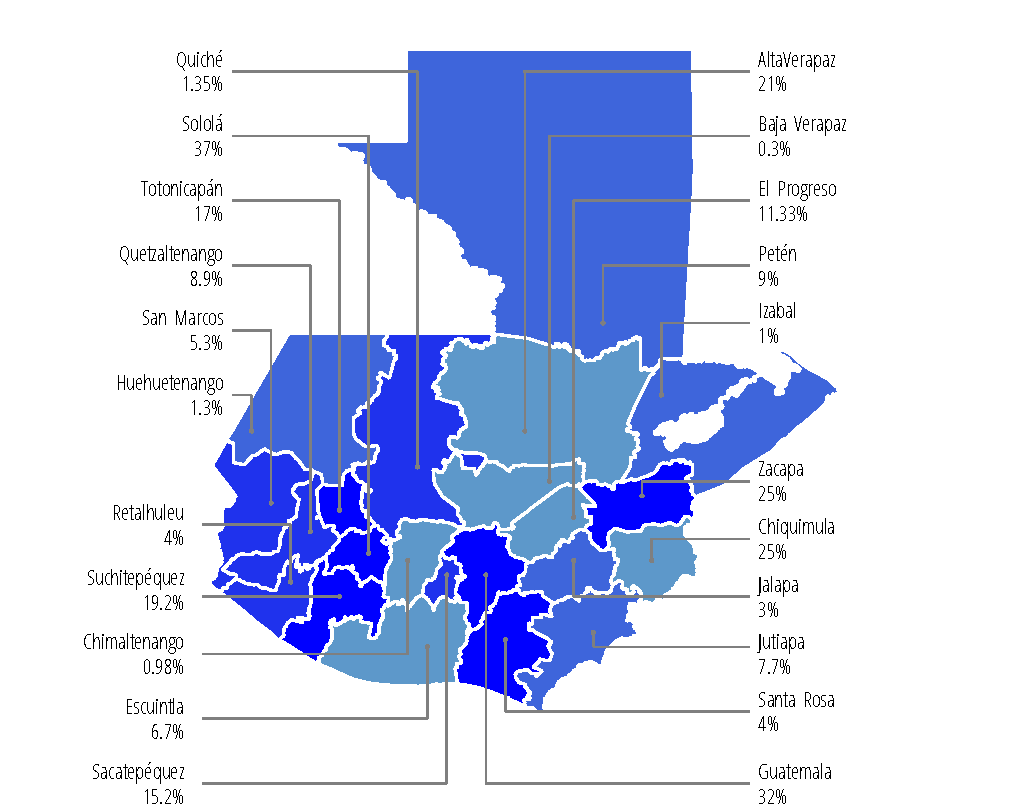
\includegraphics[width=52\cuadri]{graficas/1_05.pdf}}%
{%
 Instituto Nacional de Estadística} %
 
 \cajota{%
Pobreza total en los departamentos en 2014}%
{%
 La línea de pobreza extrema representa el costo de adquirir la cantidad mínima de calorías recomendadas. Para el año 2000, la línea de pobreza era de 1,911 quetzales, que ajustado a precios de 2014, era equivalente a Q4,427. La línea de pobreza para 2006, ajustada a 2014 era equivalente a 4,380 quetzales. Esto quiere decir que aproximadamente la línea de pobreza extrema aumentó en 1,370 quetzales entre 2006 y 2014.  }%
{%
 Incidencia de pobreza total por departamento 2014} %
{%
 Por departamento, Encovi 2014, en porcentaje} %
{%
 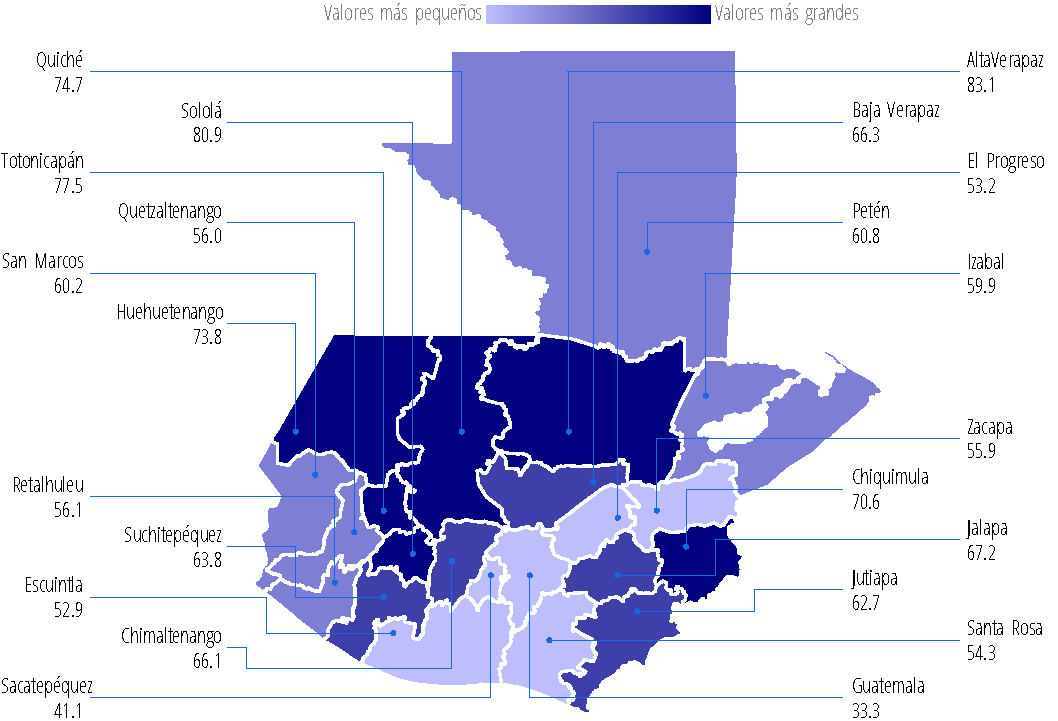
\includegraphics[width=52\cuadri]{graficas/1_06.pdf}}%
{%
 Instituto Nacional de Estadística} %
 
 \cajota{%
Cambio de la pobreza total }%
{%
 Los resultados positivos de la comparación entre 2006 y 2014, significan un aumento de la pobreza en este período. Se puede observar que el mayor aumento entre estos dos años, se dio en el departamento de Guatemala, con un aumento de 17 puntos porcentuales en la pobreza. Le siguen los departamentos de Jutiapa, Quetzaltenango, Escuintla, El Progreso y Chiquimula, con un aumento de más de 10 puntos porcentuales. Los departamentos que muestran una reducción de la pobreza son Quiché, San Marcos, Baja Verapaz y Santa Rosa. }%
{%
 Incidencia de pobreza extrema nacional} %
{%
 Por departamento, Encovi 2006 y 2014, en puntos porcentuales} %
{%
 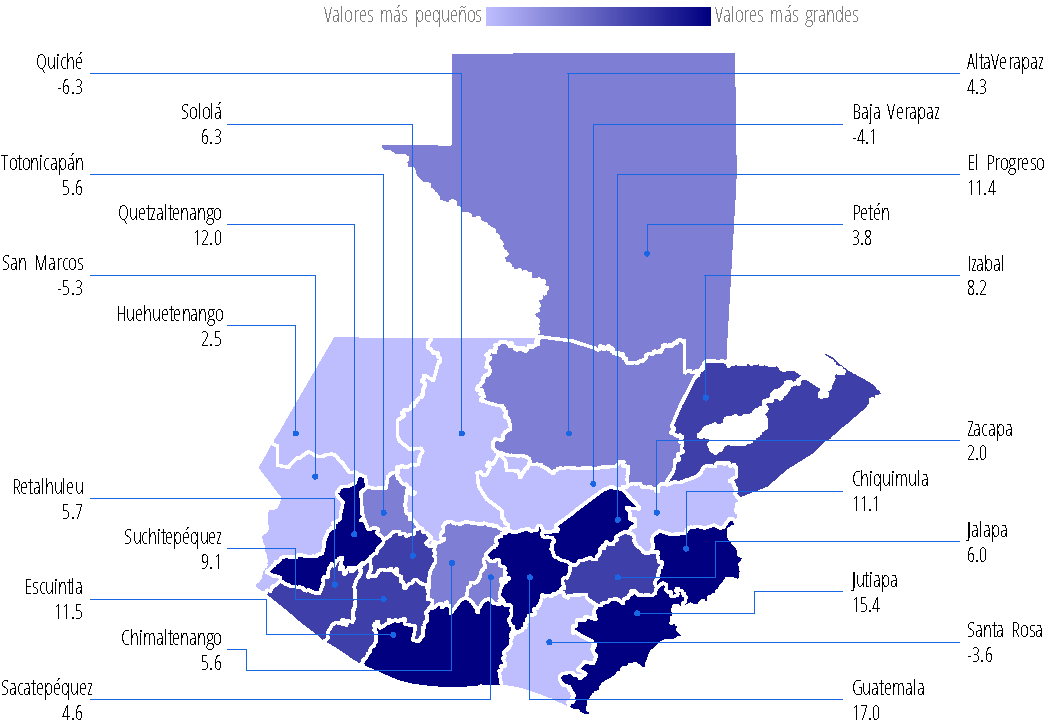
\includegraphics[width=52\cuadri]{graficas/1_07.pdf}}%
{%
 Instituto Nacional de Estadística} %
 
 \cajita{%
Línea de pobreza extrema}%
{%
 La pobreza extrema es mayor en la población indígena. Para el año 2000, más de la cuarta parte de la población indígena se encontraba en pobreza extrema, se puede observar que entre 2000 y 2006 el nivel de pobreza se mantuvo, y aumentó a casi 40\% en 2014. Para la población no indígena, la pobreza extrema aumentó de cinco puntos porcentuales, de 7.8\% a 12.8\% entre 2000 y 2014.}%
{%
 Líneas de pobreza extrema nacional} %
{%
 Républica de Guatemala, Encovi 2000, 2006 y 2014, en quetzales de cada año} %
{%
 \begin{tikzpicture}[x=1pt,y=1pt]  % Created by tikzDevice version 0.9 on 2015-11-26 21:53:16
% !TEX encoding = UTF-8 Unicode
\definecolor{fillColor}{RGB}{255,255,255}
\path[use as bounding box,fill=fillColor,fill opacity=0.00] (0,0) rectangle (289.08,198.74);
\begin{scope}
\path[clip] (  0.00,  0.00) rectangle (289.08,198.74);

\path[] (  0.00,  0.00) rectangle (289.08,198.74);
\end{scope}
\begin{scope}
\path[clip] (  0.00,  0.00) rectangle (289.08,198.74);

\path[] (  7.11, 20.62) rectangle (289.08,174.77);

\path[] ( 47.39, 20.62) --
	( 47.39,174.77);

\path[] (114.53, 20.62) --
	(114.53,174.77);

\path[] (181.66, 20.62) --
	(181.66,174.77);

\path[] (248.80, 20.62) --
	(248.80,174.77);
\definecolor{drawColor}{RGB}{0,0,255}
\definecolor{fillColor}{RGB}{0,0,255}

\path[draw=drawColor,line width= 0.6pt,line join=round,fill=fillColor] ( 18.86, 20.62) rectangle ( 45.72, 38.49);
\definecolor{drawColor}{RGB}{157,187,255}
\definecolor{fillColor}{RGB}{157,187,255}

\path[draw=drawColor,line width= 0.6pt,line join=round,fill=fillColor] ( 49.07, 20.62) rectangle ( 75.93,170.52);
\definecolor{drawColor}{RGB}{0,0,255}
\definecolor{fillColor}{RGB}{0,0,255}

\path[draw=drawColor,line width= 0.6pt,line join=round,fill=fillColor] ( 86.00, 20.62) rectangle (112.85, 54.27);
\definecolor{drawColor}{RGB}{157,187,255}
\definecolor{fillColor}{RGB}{157,187,255}

\path[draw=drawColor,line width= 0.6pt,line join=round,fill=fillColor] (116.21, 20.62) rectangle (143.06,174.77);
\definecolor{drawColor}{RGB}{0,0,255}
\definecolor{fillColor}{RGB}{0,0,255}

\path[draw=drawColor,line width= 0.6pt,line join=round,fill=fillColor] (153.13, 20.62) rectangle (179.99, 52.58);
\definecolor{drawColor}{RGB}{157,187,255}
\definecolor{fillColor}{RGB}{157,187,255}

\path[draw=drawColor,line width= 0.6pt,line join=round,fill=fillColor] (183.34, 20.62) rectangle (210.20,153.85);
\definecolor{drawColor}{RGB}{0,0,255}
\definecolor{fillColor}{RGB}{0,0,255}

\path[draw=drawColor,line width= 0.6pt,line join=round,fill=fillColor] (220.27, 20.62) rectangle (247.12, 20.62);
\definecolor{drawColor}{RGB}{157,187,255}
\definecolor{fillColor}{RGB}{157,187,255}

\path[draw=drawColor,line width= 0.6pt,line join=round,fill=fillColor] (250.48, 20.62) rectangle (277.33, 20.62);
\definecolor{drawColor}{RGB}{0,0,0}

\path[draw=drawColor,line width= 0.6pt,line join=round] (  7.11, 20.62) -- (289.08, 20.62);

\node[text=drawColor,anchor=base,inner sep=0pt, outer sep=0pt, scale=  0.82] at ( 32.29, 41.71) {2.8};

\node[text=drawColor,anchor=base,inner sep=0pt, outer sep=0pt, scale=  0.82] at ( 62.50,173.75) {23.8};

\node[text=drawColor,anchor=base,inner sep=0pt, outer sep=0pt, scale=  0.82] at ( 99.42, 57.49) {5.3};

\node[text=drawColor,anchor=base,inner sep=0pt, outer sep=0pt, scale=  0.82] at (129.63,177.99) {24.4};

\node[text=drawColor,anchor=base,inner sep=0pt, outer sep=0pt, scale=  0.82] at (166.56, 55.80) {5.1};

\node[text=drawColor,anchor=base,inner sep=0pt, outer sep=0pt, scale=  0.82] at (196.77,157.08) {21.1};

\node[text=drawColor,anchor=base,inner sep=0pt, outer sep=0pt, scale=  0.82] at (233.69, 23.84) {0.0};

\node[text=drawColor,anchor=base,inner sep=0pt, outer sep=0pt, scale=  0.82] at (263.90, 23.84) {0.0};

\path[] (  7.11, 20.62) rectangle (289.08,174.77);
\end{scope}
\begin{scope}
\path[clip] (  0.00,  0.00) rectangle (289.08,198.74);

\path[] (  7.11, 20.62) --
	(  7.11,174.77);
\end{scope}
\begin{scope}
\path[clip] (  0.00,  0.00) rectangle (289.08,198.74);

\path[] (  7.11, 20.62) --
	(289.08, 20.62);
\end{scope}
\begin{scope}
\path[clip] (  0.00,  0.00) rectangle (289.08,198.74);

\path[] ( 47.39, 16.35) --
	( 47.39, 20.62);

\path[] (114.53, 16.35) --
	(114.53, 20.62);

\path[] (181.66, 16.35) --
	(181.66, 20.62);

\path[] (248.80, 16.35) --
	(248.80, 20.62);
\end{scope}
\begin{scope}
\path[clip] (  0.00,  0.00) rectangle (289.08,198.74);
\definecolor{drawColor}{RGB}{0,0,0}

\node[text=drawColor,anchor=base,inner sep=0pt, outer sep=0pt, scale=  1.00] at ( 47.39,  5.69) {2000};

\node[text=drawColor,anchor=base,inner sep=0pt, outer sep=0pt, scale=  1.00] at (114.53,  5.69) {2006};

\node[text=drawColor,anchor=base,inner sep=0pt, outer sep=0pt, scale=  1.00] at (181.66,  5.69) {2011};

\node[text=drawColor,anchor=base,inner sep=0pt, outer sep=0pt, scale=  1.00] at (248.80,  5.69) {2014};
\end{scope}
\begin{scope}
\path[clip] (  0.00,  0.00) rectangle (289.08,198.74);
\coordinate (apoyo) at (57.27,191.13);
\coordinate (longitudFicticia) at (7.11,7.61);
\coordinate (longitud) at (7.11,7.11);
\coordinate (desX) at (142.24,0);
\coordinate (desY) at (0,0.25);
\definecolor[named]{ct1}{HTML}{
0000FF
}
\definecolor[named]{ct2}{HTML}{
9DBBFF
}
\definecolor[named]{ctb1}{HTML}{
0000FF
}
\definecolor[named]{ctb2}{HTML}{
9DBBFF
}
\path [fill=none] (apoyo) rectangle ($(apoyo)+(longitudFicticia)$)
node [xshift=0.3cm,inner sep=0pt, outer sep=0pt,midway,right,scale = 0.9]{Urbana};
\draw [color = ctb1,fill=ct1] ( $(apoyo)  + (desY) $) rectangle ($(apoyo)+ (desY) +(longitud)$);
\path [fill=none] ($(apoyo)+(desX)$) rectangle ($(apoyo)+(desX)+(longitudFicticia)$)
node [xshift=0.3cm,inner sep=0pt, outer sep=0pt,midway,right,scale = 0.9]{Rural};
\draw [color = ctb2 ,fill=ct2] ( $(apoyo)  + (desY) + (desX) $) rectangle ($(apoyo)+ (desY)+ (desX) +(longitud)$);
\end{scope}
  \end{tikzpicture}}%
{%
 Instituto Nacional de Estadística} %
 
 \cajita{%
Pobreza extrema}%
{%
 Para el año 2000, la pobreza extrema en el área urbana era menor al 3\%, mientras que en el área rural, era ocho veces mayor que en el área urbana. Entre 2000 y 2014, se advierte un aumento de la pobreza extrema para ambos grupos. Aunque en puntos porcentuales fue mayor el aumento para el área rural, el aumento de pobreza en el área urbana fue casi cuatro veces lo observado para el año 2000.}%
{%
 Incidencia de pobreza extrema nacional} %
{%
 Républica de Guatemala, serie histórica por Encovi, en porcentaje} %
{%
 \begin{tikzpicture}[x=1pt,y=1pt]  % Created by tikzDevice version 0.9 on 2015-11-26 22:20:41
% !TEX encoding = UTF-8 Unicode
\definecolor{fillColor}{RGB}{255,255,255}
\path[use as bounding box,fill=fillColor,fill opacity=0.00] (0,0) rectangle (289.08,198.74);
\begin{scope}
\path[clip] (  0.00,  0.00) rectangle (289.08,198.74);

\path[] (  0.00,  0.00) rectangle (289.08,198.74);
\end{scope}
\begin{scope}
\path[clip] (  0.00,  0.00) rectangle (289.08,198.74);

\path[] (  7.11, 20.62) rectangle (289.08,174.77);

\path[] ( 59.98, 20.62) --
	( 59.98,174.77);

\path[] (148.10, 20.62) --
	(148.10,174.77);

\path[] (236.21, 20.62) --
	(236.21,174.77);
\definecolor{drawColor}{RGB}{0,0,255}
\definecolor{fillColor}{RGB}{0,0,255}

\path[draw=drawColor,line width= 0.6pt,line join=round,fill=fillColor] ( 22.53, 20.62) rectangle ( 57.78, 33.00);
\definecolor{drawColor}{RGB}{157,187,255}
\definecolor{fillColor}{RGB}{157,187,255}

\path[draw=drawColor,line width= 0.6pt,line join=round,fill=fillColor] ( 62.18, 20.62) rectangle ( 97.43,124.49);
\definecolor{drawColor}{RGB}{0,0,255}
\definecolor{fillColor}{RGB}{0,0,255}

\path[draw=drawColor,line width= 0.6pt,line join=round,fill=fillColor] (110.65, 20.62) rectangle (145.89, 43.93);
\definecolor{drawColor}{RGB}{157,187,255}
\definecolor{fillColor}{RGB}{157,187,255}

\path[draw=drawColor,line width= 0.6pt,line join=round,fill=fillColor] (150.30, 20.62) rectangle (185.55,127.43);
\definecolor{drawColor}{RGB}{0,0,255}
\definecolor{fillColor}{RGB}{0,0,255}

\path[draw=drawColor,line width= 0.6pt,line join=round,fill=fillColor] (198.76, 20.62) rectangle (234.01, 69.70);
\definecolor{drawColor}{RGB}{157,187,255}
\definecolor{fillColor}{RGB}{157,187,255}

\path[draw=drawColor,line width= 0.6pt,line join=round,fill=fillColor] (238.41, 20.62) rectangle (273.66,174.77);
\definecolor{drawColor}{RGB}{0,0,0}

\path[draw=drawColor,line width= 0.6pt,line join=round] (  7.11, 20.62) -- (289.08, 20.62);

\node[text=drawColor,anchor=base,inner sep=0pt, outer sep=0pt, scale=  0.82] at ( 40.16, 36.23) {2.8};

\node[text=drawColor,anchor=base,inner sep=0pt, outer sep=0pt, scale=  0.82] at ( 79.81,127.72) {23.8};

\node[text=drawColor,anchor=base,inner sep=0pt, outer sep=0pt, scale=  0.82] at (128.27, 47.16) {5.3};

\node[text=drawColor,anchor=base,inner sep=0pt, outer sep=0pt, scale=  0.82] at (167.92,130.66) {24.4};

\node[text=drawColor,anchor=base,inner sep=0pt, outer sep=0pt, scale=  0.82] at (216.39, 72.92) {11.2};

\node[text=drawColor,anchor=base,inner sep=0pt, outer sep=0pt, scale=  0.82] at (256.04,177.99) {35.3};

\path[] (  7.11, 20.62) rectangle (289.08,174.77);
\end{scope}
\begin{scope}
\path[clip] (  0.00,  0.00) rectangle (289.08,198.74);

\path[] (  7.11, 20.62) --
	(  7.11,174.77);
\end{scope}
\begin{scope}
\path[clip] (  0.00,  0.00) rectangle (289.08,198.74);

\path[] (  7.11, 20.62) --
	(289.08, 20.62);
\end{scope}
\begin{scope}
\path[clip] (  0.00,  0.00) rectangle (289.08,198.74);

\path[] ( 59.98, 16.35) --
	( 59.98, 20.62);

\path[] (148.10, 16.35) --
	(148.10, 20.62);

\path[] (236.21, 16.35) --
	(236.21, 20.62);
\end{scope}
\begin{scope}
\path[clip] (  0.00,  0.00) rectangle (289.08,198.74);
\definecolor{drawColor}{RGB}{0,0,0}

\node[text=drawColor,anchor=base,inner sep=0pt, outer sep=0pt, scale=  1.00] at ( 59.98,  5.69) {2000};

\node[text=drawColor,anchor=base,inner sep=0pt, outer sep=0pt, scale=  1.00] at (148.10,  5.69) {2006};

\node[text=drawColor,anchor=base,inner sep=0pt, outer sep=0pt, scale=  1.00] at (236.21,  5.69) {2014};
\end{scope}
\begin{scope}
\path[clip] (  0.00,  0.00) rectangle (289.08,198.74);
\coordinate (apoyo) at (57.27,191.13);
\coordinate (longitudFicticia) at (7.11,7.61);
\coordinate (longitud) at (7.11,7.11);
\coordinate (desX) at (142.24,0);
\coordinate (desY) at (0,0.25);
\definecolor[named]{ct1}{HTML}{
0000FF
}
\definecolor[named]{ct2}{HTML}{
9DBBFF
}
\definecolor[named]{ctb1}{HTML}{
0000FF
}
\definecolor[named]{ctb2}{HTML}{
9DBBFF
}
\path [fill=none] (apoyo) rectangle ($(apoyo)+(longitudFicticia)$)
node [xshift=0.3cm,inner sep=0pt, outer sep=0pt,midway,right,scale = 0.9]{Urbana};
\draw [color = ctb1,fill=ct1] ( $(apoyo)  + (desY) $) rectangle ($(apoyo)+ (desY) +(longitud)$);
\path [fill=none] ($(apoyo)+(desX)$) rectangle ($(apoyo)+(desX)+(longitudFicticia)$)
node [xshift=0.3cm,inner sep=0pt, outer sep=0pt,midway,right,scale = 0.9]{Rural};
\draw [color = ctb2 ,fill=ct2] ( $(apoyo)  + (desY) + (desX) $) rectangle ($(apoyo)+ (desY)+ (desX) +(longitud)$);
\end{scope}
  \end{tikzpicture}}%
{%
 Instituto Nacional de Estadística} %
 
 \cajita{%
Pobreza extrema por etnicidad}%
{%
  Para el año 2000, el 27.1\%  de la población indígena se encontraba en pobreza extrema. Se puede observar que entre 2000 y 2006 el nivel de pobreza se mantuvo, pero aumentó en  casi  12 puntos porcentuales en 2014.
 
  Para la población no indígena, la pobreza extrema aumentó de cinco puntos porcentuales, de 7.8\% a 12.8\% entre 2000 y 2014.}%
{%
 Incidencia de pobreza extrema por departamento} %
{%
 República de Guatemala, Encovi 2014 en porcentaje} %
{%
 \begin{tikzpicture}[x=1pt,y=1pt]  % Created by tikzDevice version 0.7.0 on 2015-11-27 11:12:38
% !TEX encoding = UTF-8 Unicode
\definecolor[named]{fillColor}{rgb}{1.00,1.00,1.00}
\path[use as bounding box,fill=fillColor,fill opacity=0.00] (0,0) rectangle (289.08,198.74);
\begin{scope}
\path[clip] (  0.00,  0.00) rectangle (289.08,198.74);

\path[] (  0.00,  0.00) rectangle (289.08,198.74);
\end{scope}
\begin{scope}
\path[clip] (  0.00,  0.00) rectangle (289.08,198.74);

\path[] (  7.11, 20.62) rectangle (289.08,171.35);

\path[] ( 59.98, 20.62) --
	( 59.98,171.35);

\path[] (148.10, 20.62) --
	(148.10,171.35);

\path[] (236.21, 20.62) --
	(236.21,171.35);
\definecolor[named]{drawColor}{rgb}{0.00,0.00,1.00}
\definecolor[named]{fillColor}{rgb}{0.00,0.00,1.00}

\path[draw=drawColor,line width= 0.6pt,line join=round,fill=fillColor] ( 22.53, 20.62) rectangle ( 57.78,123.35);
\definecolor[named]{drawColor}{rgb}{0.62,0.73,1.00}
\definecolor[named]{fillColor}{rgb}{0.62,0.73,1.00}

\path[draw=drawColor,line width= 0.6pt,line join=round,fill=fillColor] ( 62.18, 20.62) rectangle ( 97.43, 50.23);
\definecolor[named]{drawColor}{rgb}{0.00,0.00,1.00}
\definecolor[named]{fillColor}{rgb}{0.00,0.00,1.00}

\path[draw=drawColor,line width= 0.6pt,line join=round,fill=fillColor] (110.65, 20.62) rectangle (145.89,124.14);
\definecolor[named]{drawColor}{rgb}{0.62,0.73,1.00}
\definecolor[named]{fillColor}{rgb}{0.62,0.73,1.00}

\path[draw=drawColor,line width= 0.6pt,line join=round,fill=fillColor] (150.30, 20.62) rectangle (185.55, 50.03);
\definecolor[named]{drawColor}{rgb}{0.00,0.00,1.00}
\definecolor[named]{fillColor}{rgb}{0.00,0.00,1.00}

\path[draw=drawColor,line width= 0.6pt,line join=round,fill=fillColor] (198.76, 20.62) rectangle (234.01,171.35);
\definecolor[named]{drawColor}{rgb}{0.62,0.73,1.00}
\definecolor[named]{fillColor}{rgb}{0.62,0.73,1.00}

\path[draw=drawColor,line width= 0.6pt,line join=round,fill=fillColor] (238.41, 20.62) rectangle (273.66, 69.32);
\definecolor[named]{drawColor}{rgb}{0.00,0.00,0.00}
\definecolor[named]{fillColor}{rgb}{0.00,0.00,0.00}

\path[draw=drawColor,line width= 0.6pt,line join=round,fill=fillColor] (  7.11, 20.62) -- (289.08, 20.62);

\node[text=drawColor,anchor=base,inner sep=0pt, outer sep=0pt, scale=  0.82] at ( 40.16,126.57) {27.1};

\node[text=drawColor,anchor=base,inner sep=0pt, outer sep=0pt, scale=  0.82] at ( 79.81, 53.45) {7.8};

\node[text=drawColor,anchor=base,inner sep=0pt, outer sep=0pt, scale=  0.82] at (128.27,127.36) {27.3};

\node[text=drawColor,anchor=base,inner sep=0pt, outer sep=0pt, scale=  0.82] at (167.92, 53.26) {7.8};

\node[text=drawColor,anchor=base,inner sep=0pt, outer sep=0pt, scale=  0.82] at (216.39,174.57) {39.8};

\node[text=drawColor,anchor=base,inner sep=0pt, outer sep=0pt, scale=  0.82] at (256.04, 72.55) {12.8};

\path[] (  7.11, 20.62) rectangle (289.08,171.35);
\end{scope}
\begin{scope}
\path[clip] (  0.00,  0.00) rectangle (289.08,198.74);

\path[] (  7.11, 20.62) --
	(  7.11,171.35);
\end{scope}
\begin{scope}
\path[clip] (  0.00,  0.00) rectangle (289.08,198.74);

\path[] (  7.11, 20.62) --
	(289.08, 20.62);
\end{scope}
\begin{scope}
\path[clip] (  0.00,  0.00) rectangle (289.08,198.74);

\path[] ( 59.98, 16.35) --
	( 59.98, 20.62);

\path[] (148.10, 16.35) --
	(148.10, 20.62);

\path[] (236.21, 16.35) --
	(236.21, 20.62);
\end{scope}
\begin{scope}
\path[clip] (  0.00,  0.00) rectangle (289.08,198.74);
\definecolor[named]{drawColor}{rgb}{0.00,0.00,0.00}

\node[text=drawColor,anchor=base,inner sep=0pt, outer sep=0pt, scale=  1.00] at ( 59.98,  5.69) {2000};

\node[text=drawColor,anchor=base,inner sep=0pt, outer sep=0pt, scale=  1.00] at (148.10,  5.69) {2006};

\node[text=drawColor,anchor=base,inner sep=0pt, outer sep=0pt, scale=  1.00] at (236.21,  5.69) {2014};
\end{scope}
\coordinate (apoyo) at (54.15,187.71);
\coordinate (longitudFicticia) at (7.11,11.03);
\coordinate (longitud) at (7.11,7.11);
\coordinate (desX) at (133.24,0);
\coordinate (desY) at (0,1.96);
\definecolor[named]{ct1}{HTML}{
0000FF
}
\definecolor[named]{ct2}{HTML}{
9DBBFF
}
\definecolor[named]{ctb1}{HTML}{
0000FF
}
\definecolor[named]{ctb2}{HTML}{
9DBBFF
}
\path [fill=none] (apoyo) rectangle ($(apoyo)+(longitudFicticia)$)
node [xshift=0.3cm,inner sep=0pt, outer sep=0pt,midway,right,scale = 0.9]{Indígena};
\draw [color = ctb1,fill=ct1] ( $(apoyo)  + (desY) $) rectangle ($(apoyo)+ (desY) +(longitud)$);
\path [fill=none] ($(apoyo)+(desX)$) rectangle ($(apoyo)+(desX)+(longitudFicticia)$)
node [xshift=0.3cm,inner sep=0pt, outer sep=0pt,midway,right,scale = 0.9]{No indígena};
\draw [color = ctb2 ,fill=ct2] ( $(apoyo)  + (desY) + (desX) $) rectangle ($(apoyo)+ (desY)+ (desX) +(longitud)$);
  \end{tikzpicture}}%
{%
 Instituto Nacional de Estadística} %
 
 \cajita{%
Pobreza extrema por área de residencia}%
{%
 La brecha de pobreza, muestra la distancia promedio a la que se encuentra la población en pobreza a la línea de pobreza total. Este indicador permite hacer una estimación del monto que sería necesario transferir a los hogares de escasos recursos, para poder salir de la pobreza.   Entre 2000 y 2006, la brecha de pobreza se redujo en 3.2 puntos porcentuales. No obstante, entre 2006 y 2014, la distancia de la población a la línea de pobreza total aumentó 22.0\%, casi el misma distancia observada que para el año 2000.}%
{%
 Incidencia de pobreza extrema por área de residencia} %
{%
 Républica de Guatemala, serie histórica por Encovi, en porcentaje} %
{%
 \begin{tikzpicture}[x=1pt,y=1pt]  % Created by tikzDevice version 0.9 on 2015-11-26 22:13:04
% !TEX encoding = UTF-8 Unicode
\definecolor{fillColor}{RGB}{255,255,255}
\path[use as bounding box,fill=fillColor,fill opacity=0.00] (0,0) rectangle (289.08,198.74);
\begin{scope}
\path[clip] (  0.00,  0.00) rectangle (289.08,198.74);

\path[] (  0.00,  0.00) rectangle (289.08,198.74);
\end{scope}
\begin{scope}
\path[clip] (  0.00,  0.00) rectangle (289.08,198.74);

\path[] (  1.64, 17.78) rectangle (280.54,191.48);

\path[] (  1.64, 22.56) --
	(280.54, 22.56);

\path[] (  1.64, 60.67) --
	(280.54, 60.67);

\path[] (  1.64, 98.77) --
	(280.54, 98.77);

\path[] (  1.64,136.88) --
	(280.54,136.88);

\path[] (  1.64,174.99) --
	(280.54,174.99);

\path[] (  1.64, 41.61) --
	(280.54, 41.61);

\path[] (  1.64, 79.72) --
	(280.54, 79.72);

\path[] (  1.64,117.83) --
	(280.54,117.83);

\path[] (  1.64,155.94) --
	(280.54,155.94);

\path[] ( 53.94, 17.78) --
	( 53.94,191.48);

\path[] (141.09, 17.78) --
	(141.09,191.48);

\path[] (228.25, 17.78) --
	(228.25,191.48);
\definecolor{drawColor}{RGB}{0,0,255}

\path[draw=drawColor,line width= 1.7pt,line join=round] ( 53.94,183.59) --
	(141.09, 62.11) --
	(228.25,156.25);
\definecolor{drawColor}{RGB}{0,0,0}

\node[text=drawColor,anchor=base,inner sep=0pt, outer sep=0pt, scale=  1.01] at ( 53.94,187.54) {22.7};

\node[text=drawColor,anchor=base,inner sep=0pt, outer sep=0pt, scale=  1.01] at (141.09, 50.24) {19.5};

\node[text=drawColor,anchor=base,inner sep=0pt, outer sep=0pt, scale=  1.01] at (228.25,160.21) {22.0};

\path[draw=drawColor,line width= 0.1pt,line join=round] (  1.64, 25.67) -- (280.54, 25.67);

\path[] (  1.64, 17.78) rectangle (280.54,191.48);
\end{scope}
\begin{scope}
\path[clip] (  0.00,  0.00) rectangle (289.08,198.74);

\path[] (  1.64, 17.78) --
	(  1.64,191.48);
\end{scope}
\begin{scope}
\path[clip] (  0.00,  0.00) rectangle (289.08,198.74);

\path[] (  0.00, 41.61) --
	(  1.64, 41.61);

\path[] (  0.00, 79.72) --
	(  1.64, 79.72);

\path[] (  0.00,117.83) --
	(  1.64,117.83);

\path[] (  0.00,155.94) --
	(  1.64,155.94);
\end{scope}
\begin{scope}
\path[clip] (  0.00,  0.00) rectangle (289.08,198.74);

\path[] (  1.64, 17.78) --
	(280.54, 17.78);
\end{scope}
\begin{scope}
\path[clip] (  0.00,  0.00) rectangle (289.08,198.74);

\path[] ( 53.94, 13.51) --
	( 53.94, 17.78);

\path[] (141.09, 13.51) --
	(141.09, 17.78);

\path[] (228.25, 13.51) --
	(228.25, 17.78);
\end{scope}
\begin{scope}
\path[clip] (  0.00,  0.00) rectangle (289.08,198.74);
\definecolor{drawColor}{RGB}{0,0,0}

\node[text=drawColor,anchor=base,inner sep=0pt, outer sep=0pt, scale=  1.00] at ( 53.94,  2.85) {2000};

\node[text=drawColor,anchor=base,inner sep=0pt, outer sep=0pt, scale=  1.00] at (141.09,  2.85) {2006};

\node[text=drawColor,anchor=base,inner sep=0pt, outer sep=0pt, scale=  1.00] at (228.25,  2.85) {2014};
\end{scope}
  \end{tikzpicture}}%
{%
 Instituto Nacional de Estadística} %
 
 \cajota{%
Pobreza extrema en los departamentos}%
{%
 En el departamento de Alta Verapaz, más de la mitad de la población se encontraba en pobreza extrema para el año 2014. Para 2006, el departamento de Alta Verapaz mostraba el mayor nivel de pobreza extrema del país, y entre 2006 y 2014 aumentó en 10 puntos porcentuales.  Los departamentos de Guatemala y Sacatepéquez, mostraban porcentajes de pobreza extrema por debajo del 10\%.}%
{%
 Incidencia de pobreza extrema por departamento} %
{%
 Républica de Guatemala, serie histórica por Encovi, en porcentaje} %
{%
 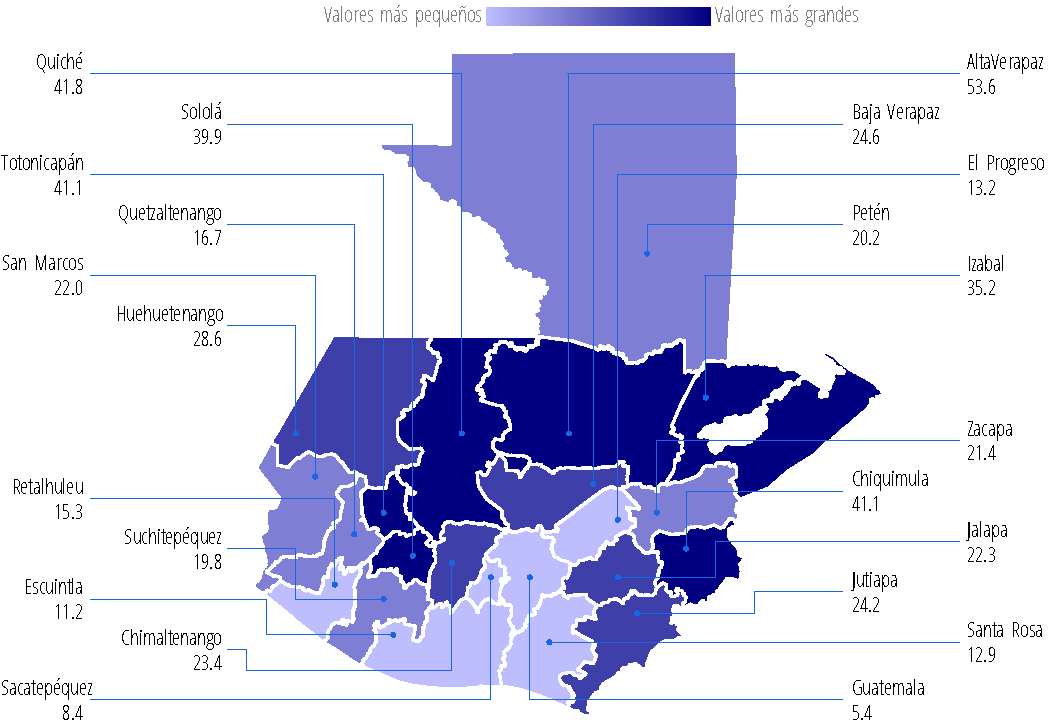
\includegraphics[width=52\cuadri]{graficas/1_12.pdf}}%
{%
 Instituto Nacional de Estadística} %
 
 \cajita{%
Brecha de pobreza total}%
{%
 La brecha de pobreza, muestra la distancia promedio a la que se encuentra la población en pobreza a la línea de pobreza total. Este indicador permite hacer una estimación del monto que sería necesario transferir a los hogares de escasos recursos, para poder salir de la pobreza.   Entre 2000 y 2006, la brecha de pobreza se redujo en 3.2 puntos porcentuales. No obstante, entre 2006 y 2014, la distancia de la población a la línea de pobreza total aumentó 22.0\%, casi el misma distancia observada que para el año 2000.}%
{%
 Brecha de la pobreza total por departamento} %
{%
 Républica de Guatemala, serie histórica por Encovi, en porcentaje} %
{%
 \begin{tikzpicture}[x=1pt,y=1pt]  % Created by tikzDevice version 0.7.0 on 2015-11-27 12:40:15
% !TEX encoding = UTF-8 Unicode
\definecolor[named]{fillColor}{rgb}{1.00,1.00,1.00}
\path[use as bounding box,fill=fillColor,fill opacity=0.00] (0,0) rectangle (289.08,198.74);
\begin{scope}
\path[clip] (  0.00,  0.00) rectangle (289.08,198.74);

\path[] (  0.00,  0.00) rectangle (289.08,198.74);
\end{scope}
\begin{scope}
\path[clip] (  0.00,  0.00) rectangle (289.08,198.74);

\path[] (  1.64, 17.78) rectangle (280.54,191.48);

\path[] (  1.64, 56.04) --
	(280.54, 56.04);

\path[] (  1.64,116.78) --
	(280.54,116.78);

\path[] (  1.64,177.51) --
	(280.54,177.51);

\path[] (  1.64, 25.67) --
	(280.54, 25.67);

\path[] (  1.64, 86.41) --
	(280.54, 86.41);

\path[] (  1.64,147.15) --
	(280.54,147.15);

\path[] ( 53.94, 17.78) --
	( 53.94,191.48);

\path[] (141.09, 17.78) --
	(141.09,191.48);

\path[] (228.25, 17.78) --
	(228.25,191.48);
\definecolor[named]{drawColor}{rgb}{0.00,0.00,1.00}

\path[draw=drawColor,line width= 1.7pt,line join=round] ( 53.94,163.70) --
	(141.09,144.34) --
	(228.25,159.34);
\definecolor[named]{drawColor}{rgb}{0.00,0.00,0.00}

\node[text=drawColor,anchor=base,inner sep=0pt, outer sep=0pt, scale=  1.01] at ( 53.94,167.66) {22.7};

\node[text=drawColor,anchor=base,inner sep=0pt, outer sep=0pt, scale=  1.01] at (141.09,132.47) {19.5};

\node[text=drawColor,anchor=base,inner sep=0pt, outer sep=0pt, scale=  1.01] at (228.25,163.30) {22.0};
\definecolor[named]{fillColor}{rgb}{0.00,0.00,0.00}

\path[draw=drawColor,line width= 0.1pt,line join=round,fill=fillColor] (  1.64, 25.67) -- (280.54, 25.67);

\path[] (  1.64, 17.78) rectangle (280.54,191.48);
\end{scope}
\begin{scope}
\path[clip] (  0.00,  0.00) rectangle (289.08,198.74);

\path[] (  1.64, 17.78) --
	(  1.64,191.48);
\end{scope}
\begin{scope}
\path[clip] (  0.00,  0.00) rectangle (289.08,198.74);

\path[] (  0.00, 25.67) --
	(  1.64, 25.67);

\path[] (  0.00, 86.41) --
	(  1.64, 86.41);

\path[] (  0.00,147.15) --
	(  1.64,147.15);
\end{scope}
\begin{scope}
\path[clip] (  0.00,  0.00) rectangle (289.08,198.74);

\path[] (  1.64, 17.78) --
	(280.54, 17.78);
\end{scope}
\begin{scope}
\path[clip] (  0.00,  0.00) rectangle (289.08,198.74);

\path[] ( 53.94, 13.51) --
	( 53.94, 17.78);

\path[] (141.09, 13.51) --
	(141.09, 17.78);

\path[] (228.25, 13.51) --
	(228.25, 17.78);
\end{scope}
\begin{scope}
\path[clip] (  0.00,  0.00) rectangle (289.08,198.74);
\definecolor[named]{drawColor}{rgb}{0.00,0.00,0.00}

\node[text=drawColor,anchor=base,inner sep=0pt, outer sep=0pt, scale=  1.00] at ( 53.94,  2.85) {2000};

\node[text=drawColor,anchor=base,inner sep=0pt, outer sep=0pt, scale=  1.00] at (141.09,  2.85) {2006};

\node[text=drawColor,anchor=base,inner sep=0pt, outer sep=0pt, scale=  1.00] at (228.25,  2.85) {2014};
\end{scope}
  \end{tikzpicture}}%
{%
 Instituto Nacional de Estadística} %
 
 \cajita{%
Brecha de pobreza extrema}%
{%
 Al combinar el indicador de incidencia y brecha de pobreza, se obtiene la severidad de la pobreza. Para el año 2000, el indicador de severidad de la pobreza era de 11.7\%, entre 2000 y 2006 se observó una reducción en la severidad de la pobreza, tanto por la reducción en el porcentaje de pobreza, como en la distancia promedio a la línea. Para 2014, el índice de severidad aumentó nuevamente, por el aumento de la pobreza, que es menor que la reducción entre 2000 y 2006, y el aumento en la brecha al mismo nivel del observado en el 2000.}%
{%
 Severidad de la pobreza total nacional} %
{%
 Républica de Guatemala, serie histórica por Encovi, en porcentaje} %
{%
 \begin{tikzpicture}[x=1pt,y=1pt]  % Created by tikzDevice version 0.9 on 2015-11-26 22:20:46
% !TEX encoding = UTF-8 Unicode
\definecolor{fillColor}{RGB}{255,255,255}
\path[use as bounding box,fill=fillColor,fill opacity=0.00] (0,0) rectangle (289.08,198.74);
\begin{scope}
\path[clip] (  0.00,  0.00) rectangle (289.08,198.74);

\path[] (  0.00,  0.00) rectangle (289.08,198.74);
\end{scope}
\begin{scope}
\path[clip] (  0.00,  0.00) rectangle (289.08,198.74);

\path[] (  1.64, 17.78) rectangle (280.54,191.48);

\path[] (  1.64, 59.45) --
	(280.54, 59.45);

\path[] (  1.64,114.75) --
	(280.54,114.75);

\path[] (  1.64,170.04) --
	(280.54,170.04);

\path[] (  1.64, 31.81) --
	(280.54, 31.81);

\path[] (  1.64, 87.10) --
	(280.54, 87.10);

\path[] (  1.64,142.39) --
	(280.54,142.39);

\path[] ( 53.94, 17.78) --
	( 53.94,191.48);

\path[] (141.09, 17.78) --
	(141.09,191.48);

\path[] (228.25, 17.78) --
	(228.25,191.48);
\definecolor{drawColor}{RGB}{0,0,255}

\path[draw=drawColor,line width= 1.7pt,line join=round] ( 53.94,183.59) --
	(141.09, 62.11) --
	(228.25,120.91);
\definecolor{drawColor}{RGB}{0,0,0}

\node[text=drawColor,anchor=base,inner sep=0pt, outer sep=0pt, scale=  1.01] at ( 53.94,187.54) {11.7};

\node[text=drawColor,anchor=base,inner sep=0pt, outer sep=0pt, scale=  1.01] at (141.09, 50.24) {9.5};

\node[text=drawColor,anchor=base,inner sep=0pt, outer sep=0pt, scale=  1.01] at (228.25,124.87) {10.6};

\path[draw=drawColor,line width= 0.1pt,line join=round] (  1.64, 25.67) -- (280.54, 25.67);

\path[] (  1.64, 17.78) rectangle (280.54,191.48);
\end{scope}
\begin{scope}
\path[clip] (  0.00,  0.00) rectangle (289.08,198.74);

\path[] (  1.64, 17.78) --
	(  1.64,191.48);
\end{scope}
\begin{scope}
\path[clip] (  0.00,  0.00) rectangle (289.08,198.74);

\path[] (  0.00, 31.81) --
	(  1.64, 31.81);

\path[] (  0.00, 87.10) --
	(  1.64, 87.10);

\path[] (  0.00,142.39) --
	(  1.64,142.39);
\end{scope}
\begin{scope}
\path[clip] (  0.00,  0.00) rectangle (289.08,198.74);

\path[] (  1.64, 17.78) --
	(280.54, 17.78);
\end{scope}
\begin{scope}
\path[clip] (  0.00,  0.00) rectangle (289.08,198.74);

\path[] ( 53.94, 13.51) --
	( 53.94, 17.78);

\path[] (141.09, 13.51) --
	(141.09, 17.78);

\path[] (228.25, 13.51) --
	(228.25, 17.78);
\end{scope}
\begin{scope}
\path[clip] (  0.00,  0.00) rectangle (289.08,198.74);
\definecolor{drawColor}{RGB}{0,0,0}

\node[text=drawColor,anchor=base,inner sep=0pt, outer sep=0pt, scale=  1.00] at ( 53.94,  2.85) {2000};

\node[text=drawColor,anchor=base,inner sep=0pt, outer sep=0pt, scale=  1.00] at (141.09,  2.85) {2006};

\node[text=drawColor,anchor=base,inner sep=0pt, outer sep=0pt, scale=  1.00] at (228.25,  2.85) {2014};
\end{scope}
  \end{tikzpicture}}%
{%
 Instituto Nacional de Estadística} %
 
 \cajota{%
Brecha de la pobreza total en los departamentos}%
{%
 El indicador de severidad de la pobreza, combina el porcentaje de pobreza y la distancia promedio a la línea de pobreza, por lo que al momento de hacer comparaciones entre departamentos, permite identificar a los que se encuentran en peores condiciones.  Se puede observar que el departamento de Alta Verapaz presenta las condiciones de pobreza más severas, seguido del departamento de Chiquimula, Totonicapán y Sololá. Mientras que en Guatemala, Sacatepéquez y Escuintla, el índice de severidad es menor, que coincide con menores porcentajes de incidencia y brecha de la pobreza. }%
{%
 Brecha de la pobreza total por departamento} %
{%
 Por departamento, Encovi 2014, en porcentaje} %
{%
 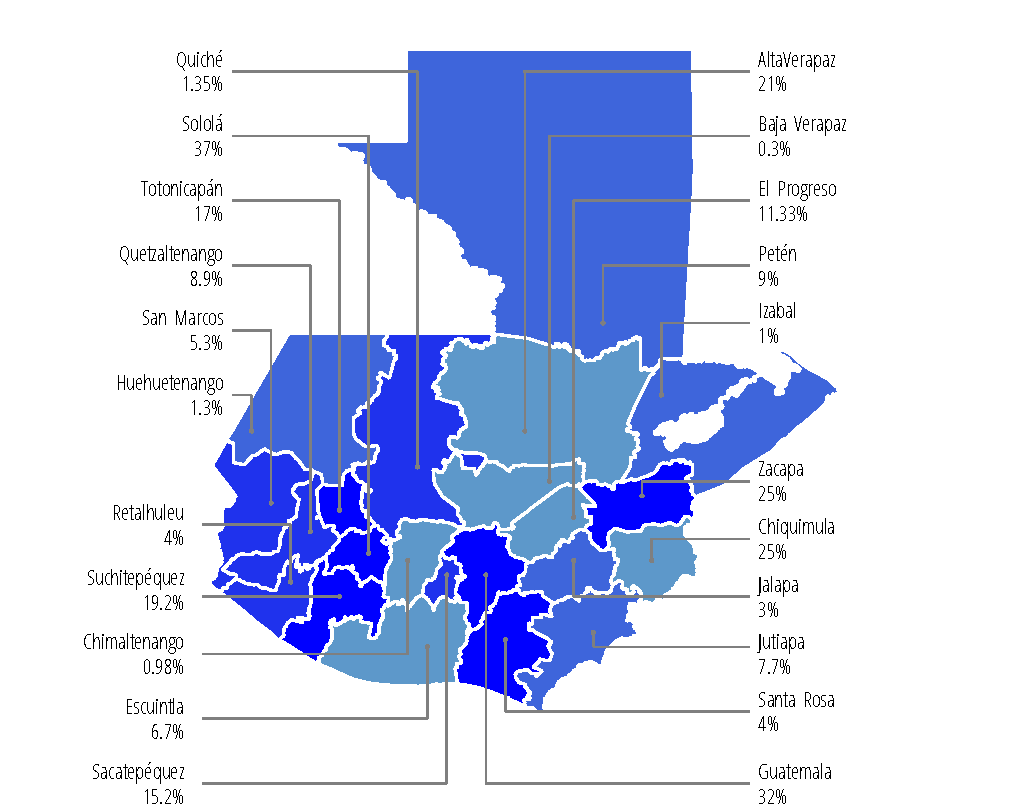
\includegraphics[width=52\cuadri]{graficas/1_15.pdf}}%
{%
 Instituto Nacional de Estadística} %
 
 \cajita{%
Severidad de la pobreza}%
{%
 Al combinar el indicador de incidencia y brecha de pobreza, se obtiene la severidad de la pobreza. Para el año 2000, el indicador de severidad de la pobreza era de 11.7\%, entre 2000 y 2006 se observó una reducción en la severidad de la pobreza, tanto por la reducción en el porcentaje de pobreza, como en la distancia promedio a la línea. Para 2014, el índice de severidad aumentó nuevamente, por el aumento de la pobreza, que es menor que la reducción entre 2000 y 2006, y el aumento en la brecha al mismo nivel del observado en el 2000.}%
{%
 Severidad de la pobreza total nacional} %
{%
 Républica de Guatemala, serie histórica por Encovi, en porcentaje} %
{%
 \begin{tikzpicture}[x=1pt,y=1pt]  % Created by tikzDevice version 0.7.0 on 2015-11-27 11:12:45
% !TEX encoding = UTF-8 Unicode
\definecolor[named]{fillColor}{rgb}{1.00,1.00,1.00}
\path[use as bounding box,fill=fillColor,fill opacity=0.00] (0,0) rectangle (289.08,198.74);
\begin{scope}
\path[clip] (  0.00,  0.00) rectangle (289.08,198.74);

\path[] (  0.00,  0.00) rectangle (289.08,198.74);
\end{scope}
\begin{scope}
\path[clip] (  0.00,  0.00) rectangle (289.08,198.74);

\path[] (  1.64, 17.78) rectangle (280.54,191.48);

\path[] (  1.64, 59.45) --
	(280.54, 59.45);

\path[] (  1.64,114.75) --
	(280.54,114.75);

\path[] (  1.64,170.04) --
	(280.54,170.04);

\path[] (  1.64, 31.81) --
	(280.54, 31.81);

\path[] (  1.64, 87.10) --
	(280.54, 87.10);

\path[] (  1.64,142.39) --
	(280.54,142.39);

\path[] ( 53.94, 17.78) --
	( 53.94,191.48);

\path[] (141.09, 17.78) --
	(141.09,191.48);

\path[] (228.25, 17.78) --
	(228.25,191.48);
\definecolor[named]{drawColor}{rgb}{0.00,0.00,1.00}

\path[draw=drawColor,line width= 1.7pt,line join=round] ( 53.94,183.59) --
	(141.09, 62.11) --
	(228.25,120.91);
\definecolor[named]{drawColor}{rgb}{0.00,0.00,0.00}

\node[text=drawColor,anchor=base,inner sep=0pt, outer sep=0pt, scale=  1.01] at ( 53.94,187.54) {11.7};

\node[text=drawColor,anchor=base,inner sep=0pt, outer sep=0pt, scale=  1.01] at (141.09, 50.24) {9.5};

\node[text=drawColor,anchor=base,inner sep=0pt, outer sep=0pt, scale=  1.01] at (228.25,124.87) {10.6};
\definecolor[named]{fillColor}{rgb}{0.00,0.00,0.00}

\path[draw=drawColor,line width= 0.1pt,line join=round,fill=fillColor] (  1.64, 25.67) -- (280.54, 25.67);

\path[] (  1.64, 17.78) rectangle (280.54,191.48);
\end{scope}
\begin{scope}
\path[clip] (  0.00,  0.00) rectangle (289.08,198.74);

\path[] (  1.64, 17.78) --
	(  1.64,191.48);
\end{scope}
\begin{scope}
\path[clip] (  0.00,  0.00) rectangle (289.08,198.74);

\path[] (  0.00, 31.81) --
	(  1.64, 31.81);

\path[] (  0.00, 87.10) --
	(  1.64, 87.10);

\path[] (  0.00,142.39) --
	(  1.64,142.39);
\end{scope}
\begin{scope}
\path[clip] (  0.00,  0.00) rectangle (289.08,198.74);

\path[] (  1.64, 17.78) --
	(280.54, 17.78);
\end{scope}
\begin{scope}
\path[clip] (  0.00,  0.00) rectangle (289.08,198.74);

\path[] ( 53.94, 13.51) --
	( 53.94, 17.78);

\path[] (141.09, 13.51) --
	(141.09, 17.78);

\path[] (228.25, 13.51) --
	(228.25, 17.78);
\end{scope}
\begin{scope}
\path[clip] (  0.00,  0.00) rectangle (289.08,198.74);
\definecolor[named]{drawColor}{rgb}{0.00,0.00,0.00}

\node[text=drawColor,anchor=base,inner sep=0pt, outer sep=0pt, scale=  1.00] at ( 53.94,  2.85) {2000};

\node[text=drawColor,anchor=base,inner sep=0pt, outer sep=0pt, scale=  1.00] at (141.09,  2.85) {2006};

\node[text=drawColor,anchor=base,inner sep=0pt, outer sep=0pt, scale=  1.00] at (228.25,  2.85) {2014};
\end{scope}
  \end{tikzpicture}}%
{%
 Instituto Nacional de Estadística} %
 
 \cajota{%
Severidad de la pobreza total en los departamentos}%
{%
   Se puede observar que el departamento de Alta Verapaz presenta las condiciones de pobreza más severas, seguido del departamento de Chiquimula, Totonicapán y Sololá. Mientras que en Guatemala, Sacatepéquez y Escuintla, el índice de severidad es menor, que coincide con menores porcentajes de incidencia y brecha de la pobreza. }%
{%
 Severidad de la pobreza total por departamento} %
{%
 Por departamento, Encovi 2014, en porcentaje} %
{%
 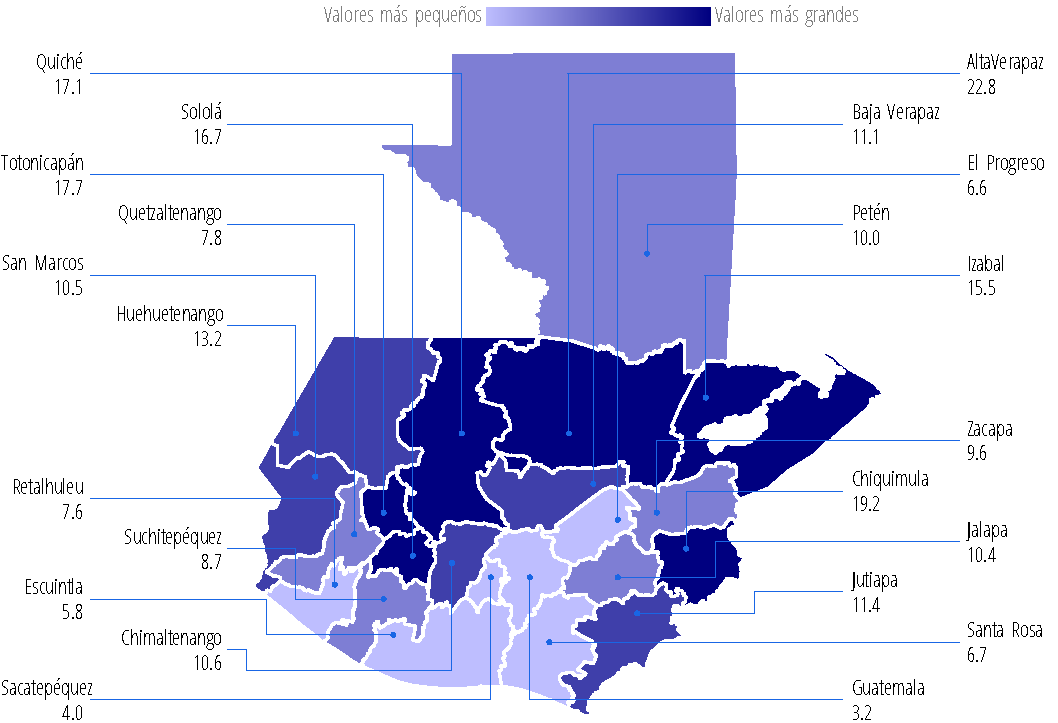
\includegraphics[width=52\cuadri]{graficas/1_17.pdf}}%
{%
 Instituto Nacional de Estadística} %
 
 \cajita{%
Pobreza en niños y adolescentes}%
{%
 Para 2014, el 68.2\% de los menores de 18 años\footnote{Según el artículo 8 del Código Civil de Guatemala: \textit{"Son mayores de edad los que han cumplido 18 años."}} habitaban en hogares pobres. Al desagregar por rangos de edad, se obtiene que el 70.2\% de los niños menores de 10 años se encontraban en pobreza. Mientas que para los niños-adolescentes entre 10 y 17 años, la pobreza era de 65.9\%.}%
{%
 Proporción de la población menor de 20 años que habitan en hogares en pobreza} %
{%
 República de Guatemala, Encovi 2014 en porcentaje} %
{%
 \begin{tikzpicture}[x=1pt,y=1pt]  % Created by tikzDevice version 0.7.0 on 2015-11-27 12:55:06
% !TEX encoding = UTF-8 Unicode
\definecolor[named]{fillColor}{rgb}{1.00,1.00,1.00}
\path[use as bounding box,fill=fillColor,fill opacity=0.00] (0,0) rectangle (289.08,198.74);
\begin{scope}
\path[clip] (  0.00,  0.00) rectangle (289.08,198.74);

\path[] (  0.00,  0.00) rectangle (289.08,198.74);
\end{scope}
\begin{scope}
\path[clip] (  0.00,  0.00) rectangle (289.08,198.74);

\path[] (  8.54, 16.35) rectangle (289.08,181.67);

\path[] ( 61.14, 16.35) --
	( 61.14,181.67);

\path[] (148.81, 16.35) --
	(148.81,181.67);

\path[] (236.48, 16.35) --
	(236.48,181.67);
\definecolor[named]{drawColor}{rgb}{0.00,0.00,1.00}
\definecolor[named]{fillColor}{rgb}{0.00,0.00,1.00}

\path[draw=drawColor,line width= 0.6pt,line join=round,fill=fillColor] ( 43.60, 23.87) rectangle ( 78.67,169.87);

\path[draw=drawColor,line width= 0.6pt,line join=round,fill=fillColor] (131.27, 23.87) rectangle (166.34,174.16);

\path[draw=drawColor,line width= 0.6pt,line join=round,fill=fillColor] (218.94, 23.87) rectangle (254.01,164.95);
\definecolor[named]{drawColor}{rgb}{0.00,0.00,0.00}
\definecolor[named]{fillColor}{rgb}{0.00,0.00,0.00}

\path[draw=drawColor,line width= 0.1pt,line join=round,fill=fillColor] (  8.54, 23.87) -- (289.08, 23.87);

\node[text=drawColor,anchor=base,inner sep=0pt, outer sep=0pt, scale=  1.01] at ( 61.14,173.83) {68.2};

\node[text=drawColor,anchor=base,inner sep=0pt, outer sep=0pt, scale=  1.01] at (148.81,178.11) {70.2};

\node[text=drawColor,anchor=base,inner sep=0pt, outer sep=0pt, scale=  1.01] at (236.48,168.91) {65.9};

\path[] (  8.54, 16.35) rectangle (289.08,181.67);
\end{scope}
\begin{scope}
\path[clip] (  0.00,  0.00) rectangle (289.08,198.74);

\path[] (  8.54, 16.35) --
	(  8.54,181.67);
\end{scope}
\begin{scope}
\path[clip] (  0.00,  0.00) rectangle (289.08,198.74);

\path[] (  8.54, 16.35) --
	(289.08, 16.35);
\end{scope}
\begin{scope}
\path[clip] (  0.00,  0.00) rectangle (289.08,198.74);

\path[] ( 61.14, 12.08) --
	( 61.14, 16.35);

\path[] (148.81, 12.08) --
	(148.81, 16.35);

\path[] (236.48, 12.08) --
	(236.48, 16.35);
\end{scope}
\begin{scope}
\path[clip] (  0.00,  0.00) rectangle (289.08,198.74);
\definecolor[named]{drawColor}{rgb}{0.00,0.00,0.00}

\node[text=drawColor,anchor=base,inner sep=0pt, outer sep=0pt, scale=  1.00] at ( 61.14,  6.04) {De 0 a 17};

\node[text=drawColor,anchor=base,inner sep=0pt, outer sep=0pt, scale=  1.00] at (148.81,  6.04) {De 0 a 9};

\node[text=drawColor,anchor=base,inner sep=0pt, outer sep=0pt, scale=  1.00] at (236.48,  6.04) {De 10 a 17};
\end{scope}
  \end{tikzpicture}}%
{%
 Instituto Nacional de Estadística} %
 
\INEchaptercarta{Desigualdad}{Para la medición de la desigualdad se utilizó el ingreso per cápita del hogar, que incluye los ingresos laborales y no laborales de sus miembros. Se estiman el coeficiente de Gini, el índice de Atkinson, el índice de Theil, y además se realizan estimaciones por quintil de ingreso. 
	
	
Los agregados de ingreso de las Encovi 2006, 2011 y 2014 son comparables, puesto que contienen las mismas variables. El agregado de ingresos para el año 2000, aunque abarca los mismos temas que para 2006, 2011 y 2014, contiene menor cantidad de variables. Las principales diferencias en comparación con las otras Encovi, es que incluye menos  variables para  el primer y segundo trabajo, pero se agregan ingresos de otro trabajo que no se contabilizan en las siguientes Encovi.
	}

 \cajita{%
Desigualdad según el coeficiente de Gini}%
{%
 \textollamada{El coeficiente de Gini permite cuantificar la distancia de la distribución a la perfecta igualdad. Su valor varía entre 0 y 1, mientras más cerca se encuentre el valor del 1, mayor será la desigualdad.} Según los resultados de la Encovi, para el año 2000 el coeficiente de Gini era 0.60. Entre 2006 y 2011, la desigualdad aumentó ligeramente de 0.56 a 0.57, respectivamente, mientras que de 2011 a 2014, se observó una reducción de la desigualdad a 0.53, por debajo de lo observado para el año 2006.}%
{%
 Coeficiente de Gini nacional} %
{%
 República de Guatemala, serie histórica por Encovi, adimensional} %
{%
 \begin{tikzpicture}[x=1pt,y=1pt]  % Created by tikzDevice version 0.7.0 on 2015-11-27 11:21:46
% !TEX encoding = UTF-8 Unicode
\definecolor[named]{fillColor}{rgb}{1.00,1.00,1.00}
\path[use as bounding box,fill=fillColor,fill opacity=0.00] (0,0) rectangle (289.08,198.74);
\begin{scope}
\path[clip] (  0.00,  0.00) rectangle (289.08,198.74);

\path[] (  0.00,  0.00) rectangle (289.08,198.74);
\end{scope}
\begin{scope}
\path[clip] (  0.00,  0.00) rectangle (289.08,198.74);

\path[] ( 12.44, 17.78) rectangle (280.54,191.48);

\path[] ( 12.44, 41.46) --
	(280.54, 41.46);

\path[] ( 12.44, 73.05) --
	(280.54, 73.05);

\path[] ( 12.44,104.63) --
	(280.54,104.63);

\path[] ( 12.44,136.21) --
	(280.54,136.21);

\path[] ( 12.44,167.80) --
	(280.54,167.80);

\path[] ( 12.44, 25.67) --
	(280.54, 25.67);

\path[] ( 12.44, 57.25) --
	(280.54, 57.25);

\path[] ( 12.44, 88.84) --
	(280.54, 88.84);

\path[] ( 12.44,120.42) --
	(280.54,120.42);

\path[] ( 12.44,152.00) --
	(280.54,152.00);

\path[] ( 12.44,183.59) --
	(280.54,183.59);

\path[] ( 50.74, 17.78) --
	( 50.74,191.48);

\path[] (114.57, 17.78) --
	(114.57,191.48);

\path[] (178.41, 17.78) --
	(178.41,191.48);

\path[] (242.24, 17.78) --
	(242.24,191.48);
\definecolor[named]{drawColor}{rgb}{0.00,0.00,1.00}

\path[draw=drawColor,line width= 1.7pt,line join=round] ( 50.74,152.94) --
	(114.57,138.59) --
	(178.41,140.92) --
	(242.24,130.29);
\definecolor[named]{drawColor}{rgb}{0.00,0.00,0.00}

\node[text=drawColor,anchor=base,inner sep=0pt, outer sep=0pt, scale=  1.01] at ( 50.74,156.90) {0.60};

\node[text=drawColor,anchor=base,inner sep=0pt, outer sep=0pt, scale=  1.01] at (114.57,126.72) {0.56};

\node[text=drawColor,anchor=base,inner sep=0pt, outer sep=0pt, scale=  1.01] at (178.41,144.88) {0.56};

\node[text=drawColor,anchor=base,inner sep=0pt, outer sep=0pt, scale=  1.01] at (242.24,118.42) {0.53};
\definecolor[named]{fillColor}{rgb}{0.00,0.00,0.00}

\path[draw=drawColor,line width= 0.1pt,line join=round,fill=fillColor] ( 12.44, 25.67) -- (280.54, 25.67);

\path[] ( 12.44, 17.78) rectangle (280.54,191.48);
\end{scope}
\begin{scope}
\path[clip] (  0.00,  0.00) rectangle (289.08,198.74);

\path[] ( 12.44, 17.78) --
	( 12.44,191.48);
\end{scope}
\begin{scope}
\path[clip] (  0.00,  0.00) rectangle (289.08,198.74);
\definecolor[named]{drawColor}{rgb}{1.00,1.00,1.00}

\node[text=drawColor,text opacity=0.00,anchor=base east,inner sep=0pt, outer sep=0pt, scale=  1.00] at (  5.32, 21.76) {0.2};

\node[text=drawColor,text opacity=0.00,anchor=base east,inner sep=0pt, outer sep=0pt, scale=  1.00] at (  5.32, 53.35) {0.3};

\node[text=drawColor,text opacity=0.00,anchor=base east,inner sep=0pt, outer sep=0pt, scale=  1.00] at (  5.32, 84.93) {0.4};

\node[text=drawColor,text opacity=0.00,anchor=base east,inner sep=0pt, outer sep=0pt, scale=  1.00] at (  5.32,116.51) {0.5};

\node[text=drawColor,text opacity=0.00,anchor=base east,inner sep=0pt, outer sep=0pt, scale=  1.00] at (  5.32,148.10) {0.6};

\node[text=drawColor,text opacity=0.00,anchor=base east,inner sep=0pt, outer sep=0pt, scale=  1.00] at (  5.32,179.68) {0.7};
\end{scope}
\begin{scope}
\path[clip] (  0.00,  0.00) rectangle (289.08,198.74);

\path[] (  8.17, 25.67) --
	( 12.44, 25.67);

\path[] (  8.17, 57.25) --
	( 12.44, 57.25);

\path[] (  8.17, 88.84) --
	( 12.44, 88.84);

\path[] (  8.17,120.42) --
	( 12.44,120.42);

\path[] (  8.17,152.00) --
	( 12.44,152.00);

\path[] (  8.17,183.59) --
	( 12.44,183.59);
\end{scope}
\begin{scope}
\path[clip] (  0.00,  0.00) rectangle (289.08,198.74);

\path[] ( 12.44, 17.78) --
	(280.54, 17.78);
\end{scope}
\begin{scope}
\path[clip] (  0.00,  0.00) rectangle (289.08,198.74);

\path[] ( 50.74, 13.51) --
	( 50.74, 17.78);

\path[] (114.57, 13.51) --
	(114.57, 17.78);

\path[] (178.41, 13.51) --
	(178.41, 17.78);

\path[] (242.24, 13.51) --
	(242.24, 17.78);
\end{scope}
\begin{scope}
\path[clip] (  0.00,  0.00) rectangle (289.08,198.74);
\definecolor[named]{drawColor}{rgb}{0.00,0.00,0.00}

\node[text=drawColor,anchor=base,inner sep=0pt, outer sep=0pt, scale=  1.00] at ( 50.74,  2.85) {2000};

\node[text=drawColor,anchor=base,inner sep=0pt, outer sep=0pt, scale=  1.00] at (114.57,  2.85) {2006};

\node[text=drawColor,anchor=base,inner sep=0pt, outer sep=0pt, scale=  1.00] at (178.41,  2.85) {2011};

\node[text=drawColor,anchor=base,inner sep=0pt, outer sep=0pt, scale=  1.00] at (242.24,  2.85) {2014};
\end{scope}
  \end{tikzpicture}}%
{%
 Instituto Nacional de Estadística} %
 
 \cajita{%
Desigualdad según el índice de Atkinson con e=1}%
{%
 \textollamada{El índice de Atkinson mide la desigualdad en términos de la pérdida de bienestar social, debido a la dispersión de los ingresos, donde $\varepsilon$ se interpreta como un parámetro de aversión a la desigualdad.} Para el año 2000, el índice de Atkinson con el parámetro de aversión a la desigualdad igual a uno, era de 0.52. Al comparar entre 2006 y 2014, se observa una pequeña reducción en el índice de 0.45 a 0.41, respectivamente.}%
{%
 Índice de Atkinson nacional, con $\varepsilon=1$} %
{%
 República de Guatemala, serie histórica por Encovi, adimensional} %
{%
 \begin{tikzpicture}[x=1pt,y=1pt]  % Created by tikzDevice version 0.7.0 on 2015-11-24 06:39:09
% !TEX encoding = UTF-8 Unicode
\definecolor[named]{fillColor}{rgb}{1.00,1.00,1.00}
\path[use as bounding box,fill=fillColor,fill opacity=0.00] (0,0) rectangle (289.08,198.74);
\begin{scope}
\path[clip] (  0.00,  0.00) rectangle (289.08,198.74);

\path[] (  0.00,  0.00) rectangle (289.08,198.74);
\end{scope}
\begin{scope}
\path[clip] (  0.00,  0.00) rectangle (289.08,198.74);

\path[] ( 16.82, 17.78) rectangle (280.54,191.48);

\path[] ( 16.82, 27.01) --
	(280.54, 27.01);

\path[] ( 16.82, 70.85) --
	(280.54, 70.85);

\path[] ( 16.82,114.68) --
	(280.54,114.68);

\path[] ( 16.82,158.52) --
	(280.54,158.52);

\path[] ( 16.82, 48.93) --
	(280.54, 48.93);

\path[] ( 16.82, 92.77) --
	(280.54, 92.77);

\path[] ( 16.82,136.60) --
	(280.54,136.60);

\path[] ( 16.82,180.44) --
	(280.54,180.44);

\path[] ( 54.49, 17.78) --
	( 54.49,191.48);

\path[] (117.28, 17.78) --
	(117.28,191.48);

\path[] (180.08, 17.78) --
	(180.08,191.48);

\path[] (242.87, 17.78) --
	(242.87,191.48);
\definecolor[named]{drawColor}{rgb}{0.00,0.00,1.00}

\path[draw=drawColor,line width= 1.7pt,line join=round] ( 54.49,183.59) --
	(117.28, 99.88) --
	(180.08,103.93) --
	(242.87, 62.11);
\definecolor[named]{drawColor}{rgb}{0.00,0.00,0.00}

\node[text=drawColor,anchor=base,inner sep=0pt, outer sep=0pt, scale=  1.01] at ( 54.49,187.54) {0.52};

\node[text=drawColor,anchor=base,inner sep=0pt, outer sep=0pt, scale=  1.01] at (117.28, 88.01) {0.45};

\node[text=drawColor,anchor=base,inner sep=0pt, outer sep=0pt, scale=  1.01] at (180.08,107.89) {0.45};

\node[text=drawColor,anchor=base,inner sep=0pt, outer sep=0pt, scale=  1.01] at (242.87, 50.24) {0.41};
\definecolor[named]{fillColor}{rgb}{0.00,0.00,0.00}

\path[draw=drawColor,line width= 0.1pt,line join=round,fill=fillColor] ( 16.82, 25.67) -- (280.54, 25.67);

\path[] ( 16.82, 17.78) rectangle (280.54,191.48);
\end{scope}
\begin{scope}
\path[clip] (  0.00,  0.00) rectangle (289.08,198.74);

\path[] ( 16.82, 17.78) --
	( 16.82,191.48);
\end{scope}
\begin{scope}
\path[clip] (  0.00,  0.00) rectangle (289.08,198.74);
\definecolor[named]{drawColor}{rgb}{1.00,1.00,1.00}

\node[text=drawColor,text opacity=0.00,anchor=base east,inner sep=0pt, outer sep=0pt, scale=  1.00] at (  9.70, 45.02) {0.40};

\node[text=drawColor,text opacity=0.00,anchor=base east,inner sep=0pt, outer sep=0pt, scale=  1.00] at (  9.70, 88.86) {0.44};

\node[text=drawColor,text opacity=0.00,anchor=base east,inner sep=0pt, outer sep=0pt, scale=  1.00] at (  9.70,132.69) {0.48};

\node[text=drawColor,text opacity=0.00,anchor=base east,inner sep=0pt, outer sep=0pt, scale=  1.00] at (  9.70,176.53) {0.52};
\end{scope}
\begin{scope}
\path[clip] (  0.00,  0.00) rectangle (289.08,198.74);

\path[] ( 12.55, 48.93) --
	( 16.82, 48.93);

\path[] ( 12.55, 92.77) --
	( 16.82, 92.77);

\path[] ( 12.55,136.60) --
	( 16.82,136.60);

\path[] ( 12.55,180.44) --
	( 16.82,180.44);
\end{scope}
\begin{scope}
\path[clip] (  0.00,  0.00) rectangle (289.08,198.74);

\path[] ( 16.82, 17.78) --
	(280.54, 17.78);
\end{scope}
\begin{scope}
\path[clip] (  0.00,  0.00) rectangle (289.08,198.74);

\path[] ( 54.49, 13.51) --
	( 54.49, 17.78);

\path[] (117.28, 13.51) --
	(117.28, 17.78);

\path[] (180.08, 13.51) --
	(180.08, 17.78);

\path[] (242.87, 13.51) --
	(242.87, 17.78);
\end{scope}
\begin{scope}
\path[clip] (  0.00,  0.00) rectangle (289.08,198.74);
\definecolor[named]{drawColor}{rgb}{0.00,0.00,0.00}

\node[text=drawColor,anchor=base,inner sep=0pt, outer sep=0pt, scale=  1.00] at ( 54.49,  2.85) {2000};

\node[text=drawColor,anchor=base,inner sep=0pt, outer sep=0pt, scale=  1.00] at (117.28,  2.85) {2006};

\node[text=drawColor,anchor=base,inner sep=0pt, outer sep=0pt, scale=  1.00] at (180.08,  2.85) {2011};

\node[text=drawColor,anchor=base,inner sep=0pt, outer sep=0pt, scale=  1.00] at (242.87,  2.85) {2014};
\end{scope}
  \end{tikzpicture}}%
{%
 Instituto Nacional de Estadística} %
 
 \cajita{%
Desigualdad según el índice de Atkinson con $\epsilon=2$}%
{%
 Cuando $\varepsilon = \mbox{2}$, el parámetro de aversión a la desigualdad aumenta y se otorga mayor peso al extremo inferior de la distribución\footnote{El índice de Atkinson con $\varepsilon = \mbox{2} $ se calcula con la fórmula: 
	\[ A = 1 - \frac{N}{\mu}\left( \sum_{i=1}^{N}\frac{1}{x_i} \right)^{-1} \]}. \\\\ Entre 2006 y 2011, el índice de Atkinson aumentó de 0.72 a 0.77, respectivamente, y de 2011 a 2014, se redujo a 0.71.  
}%
{%
 Índice de Atkinson nacional, con $\varepsilon=2$} %
{%
 República de Guatemala, serie histórica por Encovi, adimensional} %
{%
 \begin{tikzpicture}[x=1pt,y=1pt]  % Created by tikzDevice version 0.7.0 on 2015-11-27 11:35:14
% !TEX encoding = UTF-8 Unicode
\definecolor[named]{fillColor}{rgb}{1.00,1.00,1.00}
\path[use as bounding box,fill=fillColor,fill opacity=0.00] (0,0) rectangle (289.08,198.74);
\begin{scope}
\path[clip] (  0.00,  0.00) rectangle (289.08,198.74);

\path[] (  0.00,  0.00) rectangle (289.08,198.74);
\end{scope}
\begin{scope}
\path[clip] (  0.00,  0.00) rectangle (289.08,198.74);

\path[] ( 12.44, 17.78) rectangle (280.54,191.48);

\path[] ( 12.44, 65.15) --
	(280.54, 65.15);

\path[] ( 12.44,117.79) --
	(280.54,117.79);

\path[] ( 12.44,170.43) --
	(280.54,170.43);

\path[] ( 12.44, 38.83) --
	(280.54, 38.83);

\path[] ( 12.44, 91.47) --
	(280.54, 91.47);

\path[] ( 12.44,144.11) --
	(280.54,144.11);

\path[] ( 50.74, 17.78) --
	( 50.74,191.48);

\path[] (114.57, 17.78) --
	(114.57,191.48);

\path[] (178.41, 17.78) --
	(178.41,191.48);

\path[] (242.24, 17.78) --
	(242.24,191.48);
\definecolor[named]{drawColor}{rgb}{0.00,0.00,1.00}

\path[draw=drawColor,line width= 1.7pt,line join=round] ( 50.74,167.92) --
	(114.57,123.44) --
	(178.41,135.13) --
	(242.24,121.56);
\definecolor[named]{drawColor}{rgb}{0.00,0.00,0.00}

\node[text=drawColor,anchor=base,inner sep=0pt, outer sep=0pt, scale=  1.01] at ( 50.74,171.87) {0.89};

\node[text=drawColor,anchor=base,inner sep=0pt, outer sep=0pt, scale=  1.01] at (114.57,111.57) {0.72};

\node[text=drawColor,anchor=base,inner sep=0pt, outer sep=0pt, scale=  1.01] at (178.41,139.09) {0.77};

\node[text=drawColor,anchor=base,inner sep=0pt, outer sep=0pt, scale=  1.01] at (242.24,109.69) {0.71};
\definecolor[named]{fillColor}{rgb}{0.00,0.00,0.00}

\path[draw=drawColor,line width= 0.1pt,line join=round,fill=fillColor] ( 12.44, 25.67) -- (280.54, 25.67);

\path[] ( 12.44, 17.78) rectangle (280.54,191.48);
\end{scope}
\begin{scope}
\path[clip] (  0.00,  0.00) rectangle (289.08,198.74);

\path[] ( 12.44, 17.78) --
	( 12.44,191.48);
\end{scope}
\begin{scope}
\path[clip] (  0.00,  0.00) rectangle (289.08,198.74);
\definecolor[named]{drawColor}{rgb}{1.00,1.00,1.00}

\node[text=drawColor,text opacity=0.00,anchor=base east,inner sep=0pt, outer sep=0pt, scale=  1.00] at (  5.32, 34.92) {0.4};

\node[text=drawColor,text opacity=0.00,anchor=base east,inner sep=0pt, outer sep=0pt, scale=  1.00] at (  5.32, 87.56) {0.6};

\node[text=drawColor,text opacity=0.00,anchor=base east,inner sep=0pt, outer sep=0pt, scale=  1.00] at (  5.32,140.20) {0.8};
\end{scope}
\begin{scope}
\path[clip] (  0.00,  0.00) rectangle (289.08,198.74);

\path[] (  8.17, 38.83) --
	( 12.44, 38.83);

\path[] (  8.17, 91.47) --
	( 12.44, 91.47);

\path[] (  8.17,144.11) --
	( 12.44,144.11);
\end{scope}
\begin{scope}
\path[clip] (  0.00,  0.00) rectangle (289.08,198.74);

\path[] ( 12.44, 17.78) --
	(280.54, 17.78);
\end{scope}
\begin{scope}
\path[clip] (  0.00,  0.00) rectangle (289.08,198.74);

\path[] ( 50.74, 13.51) --
	( 50.74, 17.78);

\path[] (114.57, 13.51) --
	(114.57, 17.78);

\path[] (178.41, 13.51) --
	(178.41, 17.78);

\path[] (242.24, 13.51) --
	(242.24, 17.78);
\end{scope}
\begin{scope}
\path[clip] (  0.00,  0.00) rectangle (289.08,198.74);
\definecolor[named]{drawColor}{rgb}{0.00,0.00,0.00}

\node[text=drawColor,anchor=base,inner sep=0pt, outer sep=0pt, scale=  1.00] at ( 50.74,  2.85) {2000};

\node[text=drawColor,anchor=base,inner sep=0pt, outer sep=0pt, scale=  1.00] at (114.57,  2.85) {2006};

\node[text=drawColor,anchor=base,inner sep=0pt, outer sep=0pt, scale=  1.00] at (178.41,  2.85) {2011};

\node[text=drawColor,anchor=base,inner sep=0pt, outer sep=0pt, scale=  1.00] at (242.24,  2.85) {2014};
\end{scope}
  \end{tikzpicture}}%
{%
 Instituto Nacional de Estadística} %
 
 \cajita{%
Desigualdad según el índice de Theil}%
{%
   Según lo observado con las estimaciones de los índices de desigualdad anteriores, entre 2006 y 2011 hubo  un aumento de la desigualdad .\\ \\ 
 Esto es consistente con los resultados obtenidos del índice de Theil\footnote{El índice de Theil es una medida de desigualdad que está basado en la teroía de la entropía de Shannon; entre mayor sea el valor, mayor es la desigualdad. \\\\ Se calcula con la fórmula: \[ T =\frac{1}{N} \sum_{i=1}^{N}\frac{x_i}{\mu}\Logos\mbox{ln} \left(\frac{x_i}{\mu}\right) \]}, que muestran un aumento de la desigualdad en ese período. Asimismo, para el 2014, se obtiene una reducción de la desigualdad de 0.73 en 2011 a 0.60 en 2014.}%
{%
 Índice de Theil nacional} %
{%
 República de Guatemala, serie histórica por Encovi, adimensional} %
{%
 \begin{tikzpicture}[x=1pt,y=1pt]  % Created by tikzDevice version 0.7.0 on 2015-11-27 11:39:26
% !TEX encoding = UTF-8 Unicode
\definecolor[named]{fillColor}{rgb}{1.00,1.00,1.00}
\path[use as bounding box,fill=fillColor,fill opacity=0.00] (0,0) rectangle (289.08,198.74);
\begin{scope}
\path[clip] (  0.00,  0.00) rectangle (289.08,198.74);

\path[] (  0.00,  0.00) rectangle (289.08,198.74);
\end{scope}
\begin{scope}
\path[clip] (  0.00,  0.00) rectangle (289.08,198.74);

\path[] ( 12.44, 17.78) rectangle (280.54,191.48);

\path[] ( 12.44, 41.46) --
	(280.54, 41.46);

\path[] ( 12.44, 73.05) --
	(280.54, 73.05);

\path[] ( 12.44,104.63) --
	(280.54,104.63);

\path[] ( 12.44,136.21) --
	(280.54,136.21);

\path[] ( 12.44,167.80) --
	(280.54,167.80);

\path[] ( 12.44, 25.67) --
	(280.54, 25.67);

\path[] ( 12.44, 57.25) --
	(280.54, 57.25);

\path[] ( 12.44, 88.84) --
	(280.54, 88.84);

\path[] ( 12.44,120.42) --
	(280.54,120.42);

\path[] ( 12.44,152.00) --
	(280.54,152.00);

\path[] ( 12.44,183.59) --
	(280.54,183.59);

\path[] ( 50.74, 17.78) --
	( 50.74,191.48);

\path[] (114.57, 17.78) --
	(114.57,191.48);

\path[] (178.41, 17.78) --
	(178.41,191.48);

\path[] (242.24, 17.78) --
	(242.24,191.48);
\definecolor[named]{drawColor}{rgb}{0.00,0.00,1.00}

\path[draw=drawColor,line width= 1.7pt,line join=round] ( 50.74,172.06) --
	(114.57,127.71) --
	(178.41,161.21) --
	(242.24,118.98);
\definecolor[named]{drawColor}{rgb}{0.00,0.00,0.00}

\node[text=drawColor,anchor=base,inner sep=0pt, outer sep=0pt, scale=  1.01] at ( 50.74,176.01) {0.76};

\node[text=drawColor,anchor=base,inner sep=0pt, outer sep=0pt, scale=  1.01] at (114.57,115.84) {0.62};

\node[text=drawColor,anchor=base,inner sep=0pt, outer sep=0pt, scale=  1.01] at (178.41,165.17) {0.73};

\node[text=drawColor,anchor=base,inner sep=0pt, outer sep=0pt, scale=  1.01] at (242.24,107.11) {0.60};
\definecolor[named]{fillColor}{rgb}{0.00,0.00,0.00}

\path[draw=drawColor,line width= 0.1pt,line join=round,fill=fillColor] ( 12.44, 25.67) -- (280.54, 25.67);

\path[] ( 12.44, 17.78) rectangle (280.54,191.48);
\end{scope}
\begin{scope}
\path[clip] (  0.00,  0.00) rectangle (289.08,198.74);

\path[] ( 12.44, 17.78) --
	( 12.44,191.48);
\end{scope}
\begin{scope}
\path[clip] (  0.00,  0.00) rectangle (289.08,198.74);
\definecolor[named]{drawColor}{rgb}{1.00,1.00,1.00}

\node[text=drawColor,text opacity=0.00,anchor=base east,inner sep=0pt, outer sep=0pt, scale=  1.00] at (  5.32, 21.76) {0.3};

\node[text=drawColor,text opacity=0.00,anchor=base east,inner sep=0pt, outer sep=0pt, scale=  1.00] at (  5.32, 53.35) {0.4};

\node[text=drawColor,text opacity=0.00,anchor=base east,inner sep=0pt, outer sep=0pt, scale=  1.00] at (  5.32, 84.93) {0.5};

\node[text=drawColor,text opacity=0.00,anchor=base east,inner sep=0pt, outer sep=0pt, scale=  1.00] at (  5.32,116.51) {0.6};

\node[text=drawColor,text opacity=0.00,anchor=base east,inner sep=0pt, outer sep=0pt, scale=  1.00] at (  5.32,148.10) {0.7};

\node[text=drawColor,text opacity=0.00,anchor=base east,inner sep=0pt, outer sep=0pt, scale=  1.00] at (  5.32,179.68) {0.8};
\end{scope}
\begin{scope}
\path[clip] (  0.00,  0.00) rectangle (289.08,198.74);

\path[] (  8.17, 25.67) --
	( 12.44, 25.67);

\path[] (  8.17, 57.25) --
	( 12.44, 57.25);

\path[] (  8.17, 88.84) --
	( 12.44, 88.84);

\path[] (  8.17,120.42) --
	( 12.44,120.42);

\path[] (  8.17,152.00) --
	( 12.44,152.00);

\path[] (  8.17,183.59) --
	( 12.44,183.59);
\end{scope}
\begin{scope}
\path[clip] (  0.00,  0.00) rectangle (289.08,198.74);

\path[] ( 12.44, 17.78) --
	(280.54, 17.78);
\end{scope}
\begin{scope}
\path[clip] (  0.00,  0.00) rectangle (289.08,198.74);

\path[] ( 50.74, 13.51) --
	( 50.74, 17.78);

\path[] (114.57, 13.51) --
	(114.57, 17.78);

\path[] (178.41, 13.51) --
	(178.41, 17.78);

\path[] (242.24, 13.51) --
	(242.24, 17.78);
\end{scope}
\begin{scope}
\path[clip] (  0.00,  0.00) rectangle (289.08,198.74);
\definecolor[named]{drawColor}{rgb}{0.00,0.00,0.00}

\node[text=drawColor,anchor=base,inner sep=0pt, outer sep=0pt, scale=  1.00] at ( 50.74,  2.85) {2000};

\node[text=drawColor,anchor=base,inner sep=0pt, outer sep=0pt, scale=  1.00] at (114.57,  2.85) {2006};

\node[text=drawColor,anchor=base,inner sep=0pt, outer sep=0pt, scale=  1.00] at (178.41,  2.85) {2011};

\node[text=drawColor,anchor=base,inner sep=0pt, outer sep=0pt, scale=  1.00] at (242.24,  2.85) {2014};
\end{scope}
  \end{tikzpicture}}%
{%
 Instituto Nacional de Estadística} %
 
 \cajita{%
Participación del quintil más bajo}%
{%
  Para 2000, el 20\% de la población con menos recursos, captaba el 2.0\% del total de los ingresos nacionales. Al observar los resultados de las distintas Encovi, se aprecia que la participación del quintil\footnote{Un quintil es la quinta parte de una población estadística ordenada de menor a mayor en alguna característica de esta.} más bajo se ha incrementado a 3.3 \% en 2014.}%
{%
 Proporción del primer quintil de ingresos respecto del ingreso total} %
{%
 República de Guatemala, serie histórica por Encovi, en porcentaje} %
{%
 \begin{tikzpicture}[x=1pt,y=1pt]  % Created by tikzDevice version 0.9 on 2015-11-26 22:30:54
% !TEX encoding = UTF-8 Unicode
\definecolor{fillColor}{RGB}{255,255,255}
\path[use as bounding box,fill=fillColor,fill opacity=0.00] (0,0) rectangle (289.08,198.74);
\begin{scope}
\path[clip] (  0.00,  0.00) rectangle (289.08,198.74);

\path[] (  0.00,  0.00) rectangle (289.08,198.74);
\end{scope}
\begin{scope}
\path[clip] (  0.00,  0.00) rectangle (289.08,198.74);

\path[] ( 12.44, 17.78) rectangle (280.54,191.48);

\path[] ( 12.44, 41.38) --
	(280.54, 41.38);

\path[] ( 12.44, 88.16) --
	(280.54, 88.16);

\path[] ( 12.44,134.93) --
	(280.54,134.93);

\path[] ( 12.44,181.71) --
	(280.54,181.71);

\path[] ( 12.44, 18.00) --
	(280.54, 18.00);

\path[] ( 12.44, 64.77) --
	(280.54, 64.77);

\path[] ( 12.44,111.55) --
	(280.54,111.55);

\path[] ( 12.44,158.32) --
	(280.54,158.32);

\path[] ( 50.74, 17.78) --
	( 50.74,191.48);

\path[] (114.57, 17.78) --
	(114.57,191.48);

\path[] (178.41, 17.78) --
	(178.41,191.48);

\path[] (242.24, 17.78) --
	(242.24,191.48);
\definecolor{drawColor}{RGB}{0,0,255}

\path[draw=drawColor,line width= 1.7pt,line join=round] ( 50.74, 62.11) --
	(114.57,129.49) --
	(178.41,153.19) --
	(242.24,183.59);
\definecolor{drawColor}{RGB}{0,0,0}

\node[text=drawColor,anchor=base,inner sep=0pt, outer sep=0pt, scale=  1.01] at ( 50.74, 50.24) {2.0};

\node[text=drawColor,anchor=base east,inner sep=0pt, outer sep=0pt, scale=  1.01] at (112.34,129.49) {2.7};

\node[text=drawColor,anchor=base east,inner sep=0pt, outer sep=0pt, scale=  1.01] at (176.18,153.19) {2.9};

\node[text=drawColor,anchor=base,inner sep=0pt, outer sep=0pt, scale=  1.01] at (242.24,187.54) {3.3};

\path[draw=drawColor,line width= 0.1pt,line join=round] ( 12.44, 25.67) -- (280.54, 25.67);

\path[] ( 12.44, 17.78) rectangle (280.54,191.48);
\end{scope}
\begin{scope}
\path[clip] (  0.00,  0.00) rectangle (289.08,198.74);

\path[] ( 12.44, 17.78) --
	( 12.44,191.48);
\end{scope}
\begin{scope}
\path[clip] (  0.00,  0.00) rectangle (289.08,198.74);
\definecolor{drawColor}{RGB}{255,255,255}

\node[text=drawColor,text opacity=0.00,anchor=base east,inner sep=0pt, outer sep=0pt, scale=  1.00] at (  5.32, 14.09) {1.5};

\node[text=drawColor,text opacity=0.00,anchor=base east,inner sep=0pt, outer sep=0pt, scale=  1.00] at (  5.32, 60.86) {2.0};

\node[text=drawColor,text opacity=0.00,anchor=base east,inner sep=0pt, outer sep=0pt, scale=  1.00] at (  5.32,107.64) {2.5};

\node[text=drawColor,text opacity=0.00,anchor=base east,inner sep=0pt, outer sep=0pt, scale=  1.00] at (  5.32,154.41) {3.0};
\end{scope}
\begin{scope}
\path[clip] (  0.00,  0.00) rectangle (289.08,198.74);

\path[] (  8.17, 18.00) --
	( 12.44, 18.00);

\path[] (  8.17, 64.77) --
	( 12.44, 64.77);

\path[] (  8.17,111.55) --
	( 12.44,111.55);

\path[] (  8.17,158.32) --
	( 12.44,158.32);
\end{scope}
\begin{scope}
\path[clip] (  0.00,  0.00) rectangle (289.08,198.74);

\path[] ( 12.44, 17.78) --
	(280.54, 17.78);
\end{scope}
\begin{scope}
\path[clip] (  0.00,  0.00) rectangle (289.08,198.74);

\path[] ( 50.74, 13.51) --
	( 50.74, 17.78);

\path[] (114.57, 13.51) --
	(114.57, 17.78);

\path[] (178.41, 13.51) --
	(178.41, 17.78);

\path[] (242.24, 13.51) --
	(242.24, 17.78);
\end{scope}
\begin{scope}
\path[clip] (  0.00,  0.00) rectangle (289.08,198.74);
\definecolor{drawColor}{RGB}{0,0,0}

\node[text=drawColor,anchor=base,inner sep=0pt, outer sep=0pt, scale=  1.00] at ( 50.74,  2.85) {2000};

\node[text=drawColor,anchor=base,inner sep=0pt, outer sep=0pt, scale=  1.00] at (114.57,  2.85) {2006};

\node[text=drawColor,anchor=base,inner sep=0pt, outer sep=0pt, scale=  1.00] at (178.41,  2.85) {2011};

\node[text=drawColor,anchor=base,inner sep=0pt, outer sep=0pt, scale=  1.00] at (242.24,  2.85) {2014};
\end{scope}
  \end{tikzpicture}}%
{%
 Instituto Nacional de Estadística} %
 
 \cajita{%
Participación del quintil más alto}%
{%
 \textollamada{Un quintil es la quinta parte de una población estadística ordenada de menor a mayor en alguna característica de esta.} En 2014, la participación del quintil más alto era de 57.3\%, es decir, que el 20\% más rico de la población captaba más de la mitad del total de los ingresos. \\\\
Al comparar con los resultados para años anteriores, se observa que entre 2006 y 2011, hubo un aumento en la participación del quinto quintil, y de 2011 a 2014, se redujo en aproximadamente   tres puntos porcentuales.  }%
{%
 Proporción del quinto quintil de ingresos respecto del ingreso total} %
{%
 República de Guatemala, serie histórica por Encovi, en porcentaje} %
{%
 \begin{tikzpicture}[x=1pt,y=1pt]  % Created by tikzDevice version 0.7.0 on 2015-11-24 06:39:17
% !TEX encoding = UTF-8 Unicode
\definecolor[named]{fillColor}{rgb}{1.00,1.00,1.00}
\path[use as bounding box,fill=fillColor,fill opacity=0.00] (0,0) rectangle (289.08,198.74);
\begin{scope}
\path[clip] (  0.00,  0.00) rectangle (289.08,198.74);

\path[] (  0.00,  0.00) rectangle (289.08,198.74);
\end{scope}
\begin{scope}
\path[clip] (  0.00,  0.00) rectangle (289.08,198.74);

\path[] (  8.28, 17.78) rectangle (280.54,191.48);

\path[] (  8.28, 42.22) --
	(280.54, 42.22);

\path[] (  8.28, 88.73) --
	(280.54, 88.73);

\path[] (  8.28,135.23) --
	(280.54,135.23);

\path[] (  8.28,181.74) --
	(280.54,181.74);

\path[] (  8.28, 18.97) --
	(280.54, 18.97);

\path[] (  8.28, 65.48) --
	(280.54, 65.48);

\path[] (  8.28,111.98) --
	(280.54,111.98);

\path[] (  8.28,158.49) --
	(280.54,158.49);

\path[] ( 47.17, 17.78) --
	( 47.17,191.48);

\path[] (112.00, 17.78) --
	(112.00,191.48);

\path[] (176.82, 17.78) --
	(176.82,191.48);

\path[] (241.65, 17.78) --
	(241.65,191.48);
\definecolor[named]{drawColor}{rgb}{0.00,0.00,1.00}

\path[draw=drawColor,line width= 1.7pt,line join=round] ( 47.17,183.59) --
	(112.00,102.34) --
	(176.82,121.31) --
	(241.65, 62.11);
\definecolor[named]{drawColor}{rgb}{0.00,0.00,0.00}

\node[text=drawColor,anchor=base,inner sep=0pt, outer sep=0pt, scale=  1.01] at ( 47.17,187.54) {63.8};

\node[text=drawColor,anchor=base,inner sep=0pt, outer sep=0pt, scale=  1.01] at (112.00, 90.47) {59.5};

\node[text=drawColor,anchor=base,inner sep=0pt, outer sep=0pt, scale=  1.01] at (176.82,125.27) {60.5};

\node[text=drawColor,anchor=base,inner sep=0pt, outer sep=0pt, scale=  1.01] at (241.65, 50.24) {57.3};
\definecolor[named]{fillColor}{rgb}{0.00,0.00,0.00}

\path[draw=drawColor,line width= 0.1pt,line join=round,fill=fillColor] (  8.28, 25.67) -- (280.54, 25.67);

\path[] (  8.28, 17.78) rectangle (280.54,191.48);
\end{scope}
\begin{scope}
\path[clip] (  0.00,  0.00) rectangle (289.08,198.74);

\path[] (  8.28, 17.78) --
	(  8.28,191.48);
\end{scope}
\begin{scope}
\path[clip] (  0.00,  0.00) rectangle (289.08,198.74);
\definecolor[named]{drawColor}{rgb}{1.00,1.00,1.00}

\node[text=drawColor,text opacity=0.00,anchor=base east,inner sep=0pt, outer sep=0pt, scale=  1.00] at (  1.17, 15.06) {55.0};

\node[text=drawColor,text opacity=0.00,anchor=base east,inner sep=0pt, outer sep=0pt, scale=  1.00] at (  1.17, 61.57) {57.5};

\node[text=drawColor,text opacity=0.00,anchor=base east,inner sep=0pt, outer sep=0pt, scale=  1.00] at (  1.17,108.07) {60.0};

\node[text=drawColor,text opacity=0.00,anchor=base east,inner sep=0pt, outer sep=0pt, scale=  1.00] at (  1.17,154.58) {62.5};
\end{scope}
\begin{scope}
\path[clip] (  0.00,  0.00) rectangle (289.08,198.74);

\path[] (  4.01, 18.97) --
	(  8.28, 18.97);

\path[] (  4.01, 65.48) --
	(  8.28, 65.48);

\path[] (  4.01,111.98) --
	(  8.28,111.98);

\path[] (  4.01,158.49) --
	(  8.28,158.49);
\end{scope}
\begin{scope}
\path[clip] (  0.00,  0.00) rectangle (289.08,198.74);

\path[] (  8.28, 17.78) --
	(280.54, 17.78);
\end{scope}
\begin{scope}
\path[clip] (  0.00,  0.00) rectangle (289.08,198.74);

\path[] ( 47.17, 13.51) --
	( 47.17, 17.78);

\path[] (112.00, 13.51) --
	(112.00, 17.78);

\path[] (176.82, 13.51) --
	(176.82, 17.78);

\path[] (241.65, 13.51) --
	(241.65, 17.78);
\end{scope}
\begin{scope}
\path[clip] (  0.00,  0.00) rectangle (289.08,198.74);
\definecolor[named]{drawColor}{rgb}{0.00,0.00,0.00}

\node[text=drawColor,anchor=base,inner sep=0pt, outer sep=0pt, scale=  1.00] at ( 47.17,  2.85) {2000};

\node[text=drawColor,anchor=base,inner sep=0pt, outer sep=0pt, scale=  1.00] at (112.00,  2.85) {2006};

\node[text=drawColor,anchor=base,inner sep=0pt, outer sep=0pt, scale=  1.00] at (176.82,  2.85) {2011};

\node[text=drawColor,anchor=base,inner sep=0pt, outer sep=0pt, scale=  1.00] at (241.65,  2.85) {2014};
\end{scope}
  \end{tikzpicture}}%
{%
 Instituto Nacional de Estadística} %
 
 \cajita{%
Relación de ingresos del quintil más alto y más bajo}%
{%
 \textollamada[*]{La relación de ingresos del quintil más rico y el quintil más pobre se obtiene dividiendo la participación del quinto quintil  sobre la participación del primer quintil.} Para 2014, el quintil de mayores ingresos captaba 17.5 veces más que la quinta parte de la población de menos recursos.\\\\ En general, los resultados muestran una reducción en la relación de los ingresos del quintil más alto y el más bajo de 2000 a 2014. }%
{%
 Razón del quinto y primer quintil de ingresos} %
{%
 República de Guatemala, serie histórica por Encovi, adimensional} %
{%
 \begin{tikzpicture}[x=1pt,y=1pt]  % Created by tikzDevice version 0.7.0 on 2015-11-27 11:45:03
% !TEX encoding = UTF-8 Unicode
\definecolor[named]{fillColor}{rgb}{1.00,1.00,1.00}
\path[use as bounding box,fill=fillColor,fill opacity=0.00] (0,0) rectangle (289.08,198.74);
\begin{scope}
\path[clip] (  0.00,  0.00) rectangle (289.08,198.74);

\path[] (  0.00,  0.00) rectangle (289.08,198.74);
\end{scope}
\begin{scope}
\path[clip] (  0.00,  0.00) rectangle (289.08,198.74);

\path[] (  1.64, 17.78) rectangle (280.54,191.48);

\path[] (  1.64, 41.46) --
	(280.54, 41.46);

\path[] (  1.64, 73.05) --
	(280.54, 73.05);

\path[] (  1.64,104.63) --
	(280.54,104.63);

\path[] (  1.64,136.21) --
	(280.54,136.21);

\path[] (  1.64,167.80) --
	(280.54,167.80);

\path[] (  1.64, 25.67) --
	(280.54, 25.67);

\path[] (  1.64, 57.25) --
	(280.54, 57.25);

\path[] (  1.64, 88.84) --
	(280.54, 88.84);

\path[] (  1.64,120.42) --
	(280.54,120.42);

\path[] (  1.64,152.00) --
	(280.54,152.00);

\path[] (  1.64,183.59) --
	(280.54,183.59);

\path[] ( 41.49, 17.78) --
	( 41.49,191.48);

\path[] (107.89, 17.78) --
	(107.89,191.48);

\path[] (174.30, 17.78) --
	(174.30,191.48);

\path[] (240.70, 17.78) --
	(240.70,191.48);
\definecolor[named]{drawColor}{rgb}{0.00,0.00,1.00}

\path[draw=drawColor,line width= 1.7pt,line join=round] ( 41.49,167.07) --
	(107.89,102.08) --
	(174.30, 92.27) --
	(240.70, 73.23);
\definecolor[named]{drawColor}{rgb}{0.00,0.00,0.00}

\node[text=drawColor,anchor=base,inner sep=0pt, outer sep=0pt, scale=  1.01] at ( 41.49,171.02) {32.4};

\node[text=drawColor,anchor=base west,inner sep=0pt, outer sep=0pt, scale=  1.01] at (107.89,106.04) {22.1};

\node[text=drawColor,anchor=base west,inner sep=0pt, outer sep=0pt, scale=  1.01] at (174.30, 96.22) {20.5};

\node[text=drawColor,anchor=base,inner sep=0pt, outer sep=0pt, scale=  1.01] at (240.70, 61.36) {17.5};
\definecolor[named]{fillColor}{rgb}{0.00,0.00,0.00}

\path[draw=drawColor,line width= 0.1pt,line join=round,fill=fillColor] (  1.64, 25.67) -- (280.54, 25.67);

\path[] (  1.64, 17.78) rectangle (280.54,191.48);
\end{scope}
\begin{scope}
\path[clip] (  0.00,  0.00) rectangle (289.08,198.74);

\path[] (  1.64, 17.78) --
	(  1.64,191.48);
\end{scope}
\begin{scope}
\path[clip] (  0.00,  0.00) rectangle (289.08,198.74);

\path[] (  0.00, 25.67) --
	(  1.64, 25.67);

\path[] (  0.00, 57.25) --
	(  1.64, 57.25);

\path[] (  0.00, 88.84) --
	(  1.64, 88.84);

\path[] (  0.00,120.42) --
	(  1.64,120.42);

\path[] (  0.00,152.00) --
	(  1.64,152.00);

\path[] (  0.00,183.59) --
	(  1.64,183.59);
\end{scope}
\begin{scope}
\path[clip] (  0.00,  0.00) rectangle (289.08,198.74);

\path[] (  1.64, 17.78) --
	(280.54, 17.78);
\end{scope}
\begin{scope}
\path[clip] (  0.00,  0.00) rectangle (289.08,198.74);

\path[] ( 41.49, 13.51) --
	( 41.49, 17.78);

\path[] (107.89, 13.51) --
	(107.89, 17.78);

\path[] (174.30, 13.51) --
	(174.30, 17.78);

\path[] (240.70, 13.51) --
	(240.70, 17.78);
\end{scope}
\begin{scope}
\path[clip] (  0.00,  0.00) rectangle (289.08,198.74);
\definecolor[named]{drawColor}{rgb}{0.00,0.00,0.00}

\node[text=drawColor,anchor=base,inner sep=0pt, outer sep=0pt, scale=  1.00] at ( 41.49,  2.85) {2000};

\node[text=drawColor,anchor=base,inner sep=0pt, outer sep=0pt, scale=  1.00] at (107.89,  2.85) {2006};

\node[text=drawColor,anchor=base,inner sep=0pt, outer sep=0pt, scale=  1.00] at (174.30,  2.85) {2011};

\node[text=drawColor,anchor=base,inner sep=0pt, outer sep=0pt, scale=  1.00] at (240.70,  2.85) {2014};
\end{scope}
  \end{tikzpicture}}%
{%
 Instituto Nacional de Estadística} %
 
 \cajota{%
Desigualdad en los departamentos según el coeficiente de Gini }%
{%
 Al desagregar por departamento, se observa mayor desigualdad \textemdash medida por el coeficiente de Gini\footnote{El coeficiente de Gini permite cuantificar la distancia de la distribución a la perfecta igualdad. Su valor varía entre 0 y 1, mientras más cerca se encuentre el valor del 1, mayor será la desigualdad.} \textemdash en los departamentos de San Marcos (0.61), Jalapa (0.58) y Quetzaltenango (0.58). Los departamentos con menor coeficiente de Gini son Sololá (0.39),  El Progreso  (0.42) y Escuintla (0.42).}%
{%
 Coeficiente de Gini por departamento} %
{%
 Por departamento, año 2014, adimensional} %
{%
 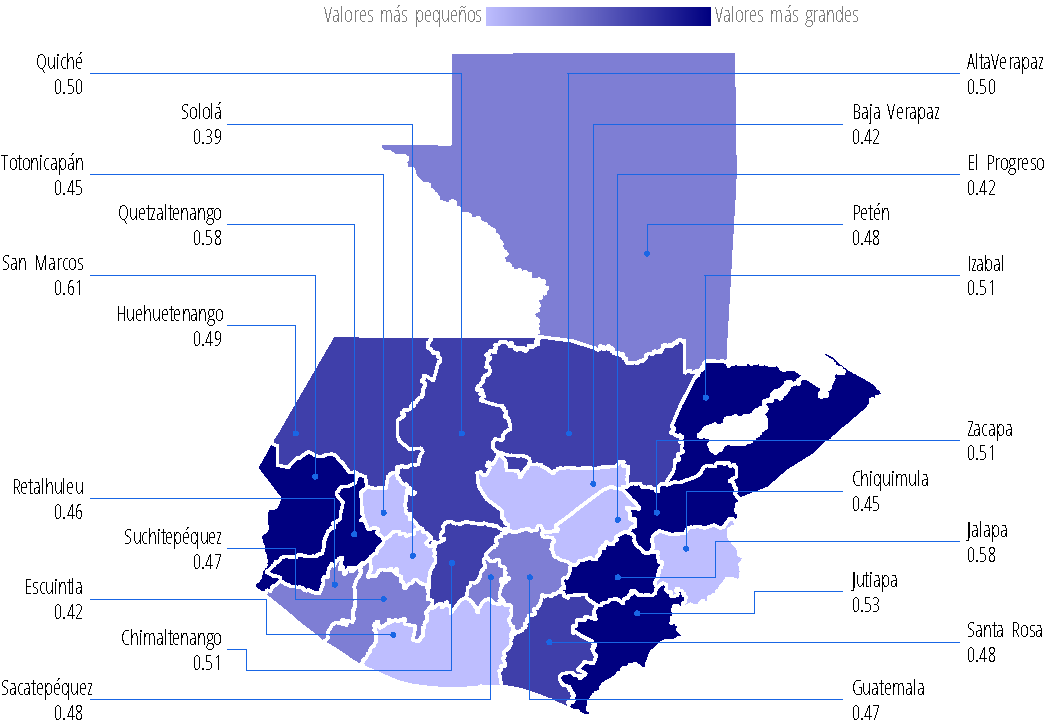
\includegraphics[width=52\cuadri]{graficas/2_08.pdf}}%
{%
 Instituto Nacional de Estadística} %
 
 \cajota{%
Desigualdad en los departamentos según el índice de Atkinson con e=1}%
{%
 Los departamentos que muestran mayor desigualdad según el índice de Atkinson\footnote{El índice de Atkinson mide la desigualdad en términos de la pérdida de bienestar social, debido a la dispersión de los ingresos, donde $\varepsilon$ se interpreta como un parámetro de aversión a la desigualdad.} (con $\varepsilon = \mbox{1}$), son San Marcos (0.52), Jalapa (0.47) y Quetzaltenago (0.46), que coinciden con los departamentos que mostraron mayor desigualdad  medida a través del coeficiente de Gini.\\\\
 Asimismo, los departamentos que muestran menor desigualdad con este índice, son Sololá, Escuintla y El progreso, con 0.24, 0.27 y 0.27, respectivamente. }%
{%
 Índice de Atkinson por departamento con $\varepsilon = 1$} %
{%
 Por departamento, año 2014, adimensional} %
{%
 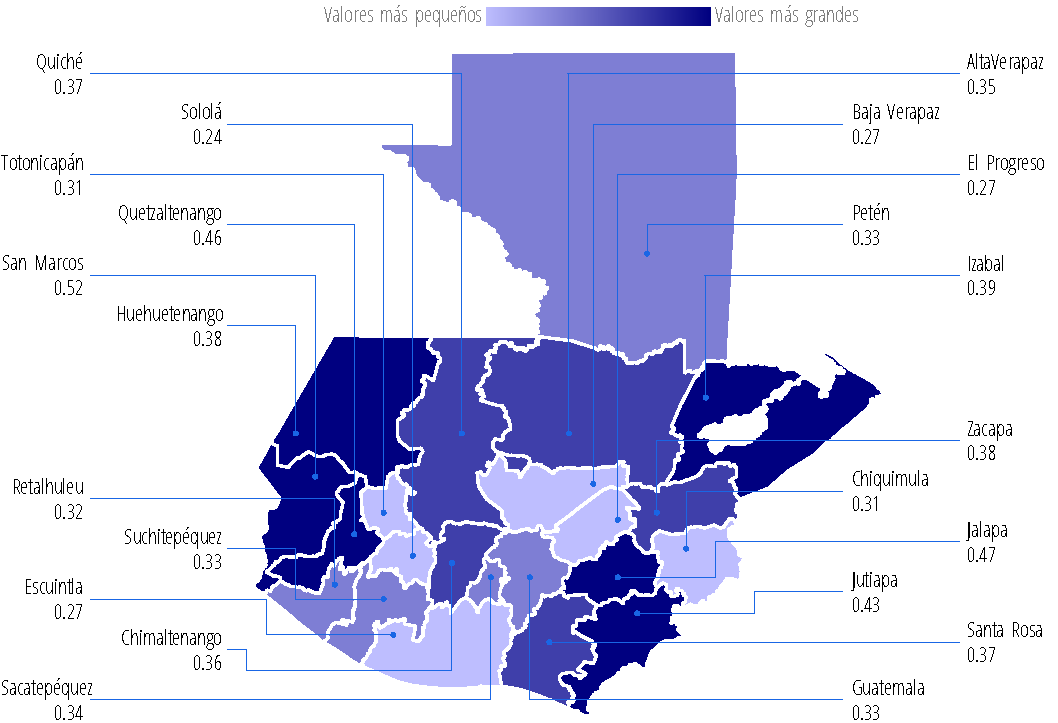
\includegraphics[width=52\cuadri]{graficas/2_09.pdf}}%
{%
 Instituto Nacional de Estadística} %
 
 \cajota{%
Desigualdad en los departamentos según el índice de Atkinson con e=2}%
{%
 Al aumentar el parámetro de aversión a la desigualdad, donde se pone mayor énfasis al extremo inferior de la distribución  ($\varepsilon = \mbox{2}$), los resultados que se venían observando se modifican. El departamento de San Marcos (0.83), sigue mostrando el mayor nivel desigualdad; no obstante, se observa cómo aumenta el índice de Atkinson para otros departamentos, como Totonicapán  que con $\varepsilon = \mbox{1}$ era uno de los menos desiguales y con $\varepsilon = \mbox{2}$ es el segundo más desigual (0.77).  \\\\ Los departamentos de Sololá (0.45), Escuintla (0.45) y El Progreso (0.48), muestran los niveles de desigualdad más bajos con el índice de Atkinson con  $\varepsilon = \mbox{2}$.}%
{%
 Índice de Atkinson por departamento con $\varepsilon = 2$} %
{%
 Por departamento, año 2014, adimensional} %
{%
 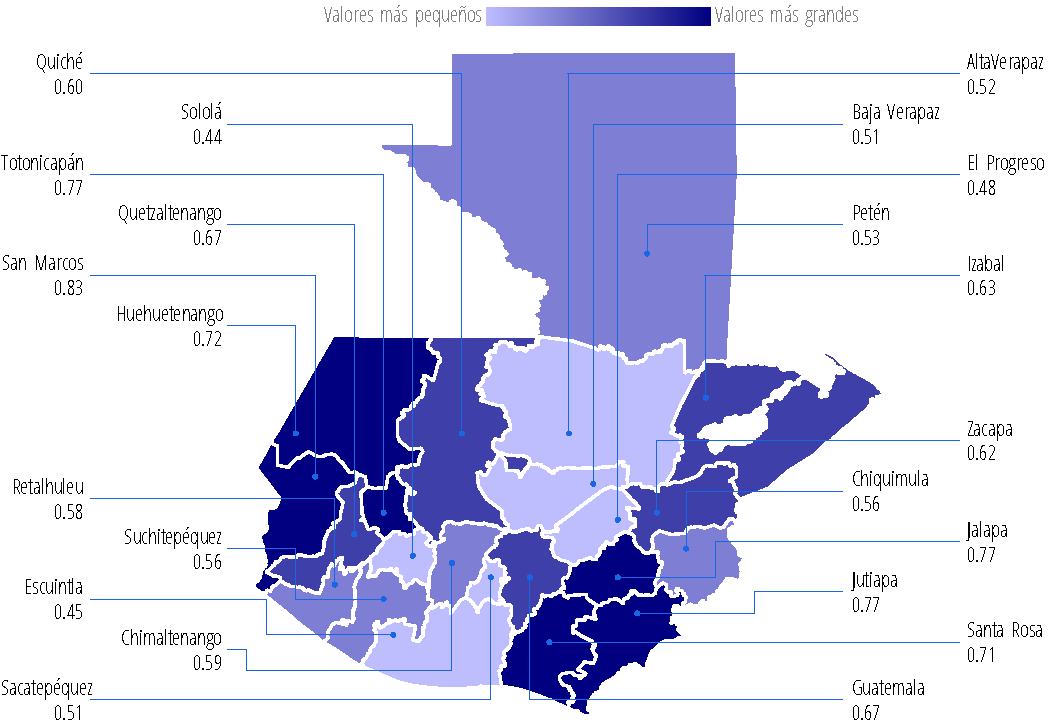
\includegraphics[width=52\cuadri]{graficas/2_10.pdf}}%
{%
 Instituto Nacional de Estadística} %
 
 \cajota{%
Desigualdad en los departamentos según el índice de Theil}%
{%
 El departamento de San Marcos (0.97) muestra el mayor nivel de desigualdad, medida a través del índice Theil\footnote{El índice de Theil es una medida de desigualdad que está basado en la entropía de Shannon; entre mayor sea el valor, mayor es la desigualdad.}, al igual que para el resto de las estimaciones anteriores;  le sigue el departamento de Quetzaltenango (0.76) y Jalapa (0.75). \\\\
 Los niveles de desigualdad más bajos, se observan en los departamentos de Baja Verapaz y El Progreso, con 0.30 ambos departamentos, y Sololá con un índice de Theil de 0.28.}%
{%
 Índice de Theil por departamento} %
{%
 Por departamento, Año 2014, adimensional} %
{%
 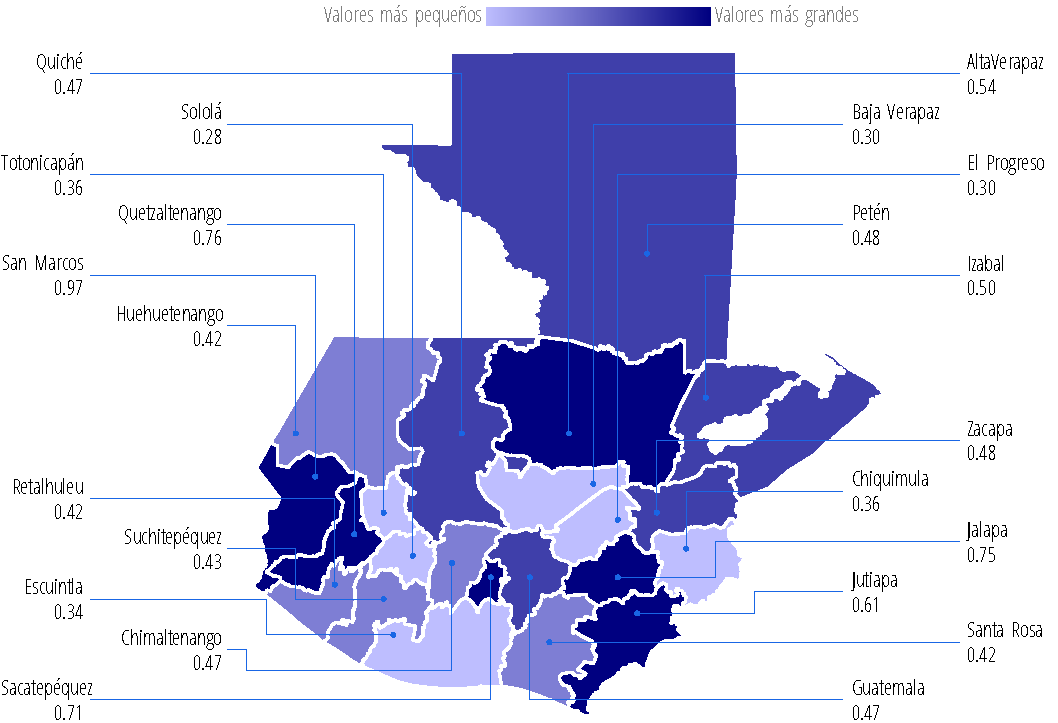
\includegraphics[width=52\cuadri]{graficas/2_11.pdf}}%
{%
 Instituto Nacional de Estadística} %
 

\INEchaptercarta{Objetivos de Desarrollo del Milenio}{
	En este capítulo se presentan los indicadores de monitoreo de los Objetivos de Desarrollo del Milenio que pueden calcularse por medio de la Encovi. 
	
	Por ejemplo se incluyen indicadores relacionados con la pobreza extrema, la alfabetización, acceso de las mujeres al trabajo remunerado en el sector no agrícola, así como de acceso a agua y saneamiento mejorados, entre otros. Cada indicador se desagrega por área urbana y rural y territorialmente por departamento.}

\INEchaptercarta{Objetivos de Desarrollo del Milenio}{}

%
%\cajota{Indicadores de los Objetivos de Desarrollo al Milenio que se monitorean con la ENCOVI}{ }{}{ }{\small
%$\ $\\[-4cm]
%\ra{1.5}$\ $\\
%\begin{tabular}{cm{4cm}m{5cm}m{5cm}}\hline
%\rowcolor{color2!15!white} &  &    &    \\[-5.9mm]
%&Descripción &  Meta     &   Indicadores     \\
%\hline
%\%\rowcolor{white}   &    &     \\[-6mm]
%\multirow{5}{*}[-2cm]{\begin{sideways} {\large Objetivo 1} \end{sideways}}&\multirow{5}{4cm}[-3cm]{Erradicar la pobreza extrema y el hambre}&\multirow{2}{5cm}[-1cm]{Meta 1A: Reducir a la mitad entre 1990 y 2015, el porcentaje de personas cuyos ingresos sean inferiores a 1 dólar por día}&Proporción de la población que se encuentra por debajo de la línea de pobreza extrema\\
%&&&Proporción del consumo nacional que corresponde al quintil más pobre de la población\\
%&&&\\
%&&\multirow{2}{5cm}[-0.5cm]{Meta 1B: Lograr empleo pleno y productivo, y trabajo decente para todos, incluyendo mujeres y jóvenes}&Relación empleo - población\\
%&&&Proporción de la población ocupada que trabaja por cuenta propia o en una empresa familiar\\
%&&\\
%\multirow{1}{*}[0.4cm]{\begin{sideways} {\large Objetivo 2} \end{sideways}} & Lograr la enseñanza primaria universal &Meta 2A: Asegurar que, para el año 2015, los niños y niñas de todo el mundo puedan terminar un ciclo completo de enseñanza primaria y &Tasa de alfabetización de las personas de 15 a 24 años, mujeres y hombres\\
%&&&\\
%\multirow{1}{*}[0.1cm]{\begin{sideways} {\large Objetivo 3} \end{sideways}} & Promover la igualdad de género y el empoderamiento de la mujer&Meta 3A: Eliminar las desigualdades entre los sexos en la enseñanza primaria y secundaria, preferiblemente para el año 2005, y en todos los niveles de la enseñanza para el año 2015&Proporción de mujeres entre los empleados remunerados en el sector no agrícola\\
%&&&\\
%
%\multirow{2}{*}[0.1cm]{\begin{sideways} {\large Objetivo 5} \end{sideways}} & \multirow{2}{4cm}[0cm]{Mejorar la salud materna}& \multirow{2}{5cm}[0cm]{Meta 5A: Reducir, entre 1990 y 2015, la mortalidad materna en tres cuartas partes} &Proporción de partos con asistencia de personal sanitario especializado\\
%
%&&&Lugar de parto para los nacimientos\\
%&&&\\
%\multirow{1}{*}[0.1cm]{\begin{sideways} {\large Objetivo 7} \end{sideways}} & Garantizar la sostenibilidad del Medio ambiente&Meta 7C: Reducir a la mitad, para el año 2015, el porcentaje de personas sin acceso sostenible al agua potable y a servicios básicos de saneamiento&Proporción de la población con acceso a fuentes mejoradas de abastecimiento de agua potable\\
%&&&Proporción de la población con acceso a servicios de saneamiento mejorados\\
%\hline
%&    &      \\[-0.05cm]
%\end{tabular}
%}{}


\cajita{Población con gastos inferiores a la línea de pobreza extrema}{ 
Este indicador muestra el porcentaje de población que no logra cubrir el costo del consumo mínimo de alimentos. 

Se puede observar que en este período, la tendencia es a una reducción en la proporción de la población que se encuentra por debajo de la línea de pobreza extrema nacional, ya que entre 2000 y 2014, este se redujo de 15.7\% a \%. 
}{Proporción de la población que se encuentra por debajo de la línea de pobreza extrema}{República de Guatemala, serie histórica por Encovi, en porcentaje}{\ \\[0mm]\begin{tikzpicture}[x=1pt,y=1pt]  % Created by tikzDevice version 0.8.1 on 2015-11-05 13:53:57
% !TEX encoding = UTF-8 Unicode
\definecolor{fillColor}{RGB}{255,255,255}
\path[use as bounding box,fill=fillColor,fill opacity=0.00] (0,0) rectangle (289.08,198.74);
\begin{scope}
\path[clip] (  0.00,  0.00) rectangle (289.08,198.74);

\path[] (  0.00,  0.00) rectangle (289.08,198.74);
\end{scope}
\begin{scope}
\path[clip] (  0.00,  0.00) rectangle (289.08,198.74);

\path[] (  1.64, 17.78) rectangle (280.54,191.48);

\path[] (  1.64, 50.76) --
	(280.54, 50.76);

\path[] (  1.64,100.94) --
	(280.54,100.94);

\path[] (  1.64,151.11) --
	(280.54,151.11);

\path[] (  1.64, 25.67) --
	(280.54, 25.67);

\path[] (  1.64, 75.85) --
	(280.54, 75.85);

\path[] (  1.64,126.02) --
	(280.54,126.02);

\path[] (  1.64,176.20) --
	(280.54,176.20);

\path[] ( 41.49, 17.78) --
	( 41.49,191.48);

\path[] (107.89, 17.78) --
	(107.89,191.48);

\path[] (174.30, 17.78) --
	(174.30,191.48);

\path[] (240.70, 17.78) --
	(240.70,191.48);
\definecolor{drawColor}{RGB}{0,0,255}

\path[draw=drawColor,line width= 1.7pt,line join=round] ( 41.49,183.59) --
	(107.89,178.21) --
	(174.30,159.14) --
	(240.70, 25.67);
\definecolor{drawColor}{RGB}{0,0,0}

\node[text=drawColor,anchor=base,inner sep=0pt, outer sep=0pt, scale=  1.01] at ( 41.49,187.54) {15.7};

\node[text=drawColor,anchor=base west,inner sep=0pt, outer sep=0pt, scale=  1.01] at (107.89,182.17) {15.2};

\node[text=drawColor,anchor=base west,inner sep=0pt, outer sep=0pt, scale=  1.01] at (174.30,163.10) {13.3};

\node[text=drawColor,anchor=base,inner sep=0pt, outer sep=0pt, scale=  1.01] at (240.70, 13.80) {0.0};

\path[draw=drawColor,line width= 0.1pt,line join=round] (  1.64, 25.67) -- (280.54, 25.67);

\path[] (  1.64, 17.78) rectangle (280.54,191.48);
\end{scope}
\begin{scope}
\path[clip] (  0.00,  0.00) rectangle (289.08,198.74);

\path[] (  1.64, 17.78) --
	(  1.64,191.48);
\end{scope}
\begin{scope}
\path[clip] (  0.00,  0.00) rectangle (289.08,198.74);

\path[] (  0.00, 25.67) --
	(  1.64, 25.67);

\path[] (  0.00, 75.85) --
	(  1.64, 75.85);

\path[] (  0.00,126.02) --
	(  1.64,126.02);

\path[] (  0.00,176.20) --
	(  1.64,176.20);
\end{scope}
\begin{scope}
\path[clip] (  0.00,  0.00) rectangle (289.08,198.74);

\path[] (  1.64, 17.78) --
	(280.54, 17.78);
\end{scope}
\begin{scope}
\path[clip] (  0.00,  0.00) rectangle (289.08,198.74);

\path[] ( 41.49, 13.51) --
	( 41.49, 17.78);

\path[] (107.89, 13.51) --
	(107.89, 17.78);

\path[] (174.30, 13.51) --
	(174.30, 17.78);

\path[] (240.70, 13.51) --
	(240.70, 17.78);
\end{scope}
\begin{scope}
\path[clip] (  0.00,  0.00) rectangle (289.08,198.74);
\definecolor{drawColor}{RGB}{0,0,0}

\node[text=drawColor,anchor=base,inner sep=0pt, outer sep=0pt, scale=  1.00] at ( 41.49,  2.85) {2000};

\node[text=drawColor,anchor=base,inner sep=0pt, outer sep=0pt, scale=  1.00] at (107.89,  2.85) {2006};

\node[text=drawColor,anchor=base,inner sep=0pt, outer sep=0pt, scale=  1.00] at (174.30,  2.85) {2011};

\node[text=drawColor,anchor=base,inner sep=0pt, outer sep=0pt, scale=  1.00] at (240.70,  2.85) {2014};
\end{scope}
  \end{tikzpicture}}{Instituto Nacional de estadística}{}
\cajita{Población con gastos inferiores a la línea de pobreza extrema por área de residencia}{ 0}{Proporción de la población que se encuentra por debajo de la línea de pobreza extrema por área de residencia}{República de Guatemala, Encovi 2014, en porcentaje}{\ \\[0mm]\begin{tikzpicture}[x=1pt,y=1pt]  % Created by tikzDevice version 0.8.1 on 2015-11-05 13:53:58
% !TEX encoding = UTF-8 Unicode
\definecolor{fillColor}{RGB}{255,255,255}
\path[use as bounding box,fill=fillColor,fill opacity=0.00] (0,0) rectangle (289.08,198.74);
\begin{scope}
\path[clip] (  0.00,  0.00) rectangle (289.08,198.74);

\path[] (  0.00,  0.00) rectangle (289.08,198.74);
\end{scope}
\begin{scope}
\path[clip] (  0.00,  0.00) rectangle (289.08,198.74);

\path[] (  8.54, 16.35) rectangle (289.08,181.67);

\path[] ( 61.14, 16.35) --
	( 61.14,181.67);

\path[] (148.81, 16.35) --
	(148.81,181.67);

\path[] (236.48, 16.35) --
	(236.48,181.67);
\definecolor{drawColor}{RGB}{0,0,255}
\definecolor{fillColor}{RGB}{0,0,255}

\path[draw=drawColor,line width= 0.6pt,line join=round,fill=fillColor] ( 43.60, 16.35) rectangle ( 78.67,126.56);

\path[draw=drawColor,line width= 0.6pt,line join=round,fill=fillColor] (131.27, 16.35) rectangle (166.34,181.67);

\path[draw=drawColor,line width= 0.6pt,line join=round,fill=fillColor] (218.94, 16.35) rectangle (254.01, 71.46);
\definecolor{drawColor}{RGB}{0,0,0}

\path[draw=drawColor,line width= 0.1pt,line join=round] (  8.54, 16.35) -- (289.08, 16.35);

\node[text=drawColor,anchor=base,inner sep=0pt, outer sep=0pt, scale=  1.01] at ( 61.14,130.52) {2};

\node[text=drawColor,anchor=base,inner sep=0pt, outer sep=0pt, scale=  1.01] at (148.81,185.63) {3};

\node[text=drawColor,anchor=base,inner sep=0pt, outer sep=0pt, scale=  1.01] at (236.48, 75.42) {1};

\path[] (  8.54, 16.35) rectangle (289.08,181.67);
\end{scope}
\begin{scope}
\path[clip] (  0.00,  0.00) rectangle (289.08,198.74);

\path[] (  8.54, 16.35) --
	(  8.54,181.67);
\end{scope}
\begin{scope}
\path[clip] (  0.00,  0.00) rectangle (289.08,198.74);

\path[] (  8.54, 16.35) --
	(289.08, 16.35);
\end{scope}
\begin{scope}
\path[clip] (  0.00,  0.00) rectangle (289.08,198.74);

\path[] ( 61.14, 12.08) --
	( 61.14, 16.35);

\path[] (148.81, 12.08) --
	(148.81, 16.35);

\path[] (236.48, 12.08) --
	(236.48, 16.35);
\end{scope}
\begin{scope}
\path[clip] (  0.00,  0.00) rectangle (289.08,198.74);
\definecolor{drawColor}{RGB}{0,0,0}

\node[text=drawColor,anchor=base,inner sep=0pt, outer sep=0pt, scale=  1.00] at ( 61.14,  6.04) {Total};

\node[text=drawColor,anchor=base,inner sep=0pt, outer sep=0pt, scale=  1.00] at (148.81,  6.04) {Urbana};

\node[text=drawColor,anchor=base,inner sep=0pt, outer sep=0pt, scale=  1.00] at (236.48,  6.04) {Rural};
\end{scope}
  \end{tikzpicture}}{Instituto Nacional de estadística}{}
\cajota{Población con gastos inferiores a la línea de pobreza extrema en los departamentos}{ 0}{Proporción de la población que se encuentra por debajo de la línea de pobreza extrema por departamento}{República de Guatemala, Encovi 2014, en porcentaje}{\ \\[0mm]\begin{tikzpicture}[x=1pt,y=1pt]  % Created by tikzDevice version 0.8.1 on 2015-11-05 13:53:58
% !TEX encoding = UTF-8 Unicode
\definecolor{fillColor}{RGB}{255,255,255}
\path[use as bounding box,fill=fillColor,fill opacity=0.00] (0,0) rectangle (289.08,198.74);
\begin{scope}
\path[clip] (  0.00,  0.00) rectangle (289.08,198.74);

\path[] (  0.00,  0.00) rectangle (289.08,198.74);
\end{scope}
\begin{scope}
\path[clip] (  0.00,  0.00) rectangle (289.08,198.74);

\path[] (  8.54, 16.35) rectangle (289.08,181.67);

\path[] ( 61.14, 16.35) --
	( 61.14,181.67);

\path[] (148.81, 16.35) --
	(148.81,181.67);

\path[] (236.48, 16.35) --
	(236.48,181.67);
\definecolor{drawColor}{RGB}{0,0,255}
\definecolor{fillColor}{RGB}{0,0,255}

\path[draw=drawColor,line width= 0.6pt,line join=round,fill=fillColor] ( 43.60, 16.35) rectangle ( 78.67,126.56);

\path[draw=drawColor,line width= 0.6pt,line join=round,fill=fillColor] (131.27, 16.35) rectangle (166.34,181.67);

\path[draw=drawColor,line width= 0.6pt,line join=round,fill=fillColor] (218.94, 16.35) rectangle (254.01, 71.46);
\definecolor{drawColor}{RGB}{0,0,0}

\path[draw=drawColor,line width= 0.1pt,line join=round] (  8.54, 16.35) -- (289.08, 16.35);

\node[text=drawColor,anchor=base,inner sep=0pt, outer sep=0pt, scale=  1.01] at ( 61.14,130.52) {2};

\node[text=drawColor,anchor=base,inner sep=0pt, outer sep=0pt, scale=  1.01] at (148.81,185.63) {3};

\node[text=drawColor,anchor=base,inner sep=0pt, outer sep=0pt, scale=  1.01] at (236.48, 75.42) {1};

\path[] (  8.54, 16.35) rectangle (289.08,181.67);
\end{scope}
\begin{scope}
\path[clip] (  0.00,  0.00) rectangle (289.08,198.74);

\path[] (  8.54, 16.35) --
	(  8.54,181.67);
\end{scope}
\begin{scope}
\path[clip] (  0.00,  0.00) rectangle (289.08,198.74);

\path[] (  8.54, 16.35) --
	(289.08, 16.35);
\end{scope}
\begin{scope}
\path[clip] (  0.00,  0.00) rectangle (289.08,198.74);

\path[] ( 61.14, 12.08) --
	( 61.14, 16.35);

\path[] (148.81, 12.08) --
	(148.81, 16.35);

\path[] (236.48, 12.08) --
	(236.48, 16.35);
\end{scope}
\begin{scope}
\path[clip] (  0.00,  0.00) rectangle (289.08,198.74);
\definecolor{drawColor}{RGB}{0,0,0}

\node[text=drawColor,anchor=base,inner sep=0pt, outer sep=0pt, scale=  1.00] at ( 61.14,  6.04) {Total};

\node[text=drawColor,anchor=base,inner sep=0pt, outer sep=0pt, scale=  1.00] at (148.81,  6.04) {Urbana};

\node[text=drawColor,anchor=base,inner sep=0pt, outer sep=0pt, scale=  1.00] at (236.48,  6.04) {Rural};
\end{scope}
  \end{tikzpicture}}{Instituto Nacional de Estadística}{}
\cajita{Consumo nacional de la quinta parte de la población más pobre}{ La participación de cada quintil en el consumo nacional, es un indicador que permite evidenciar las  desigualdades entre los distintos estratos de la población. Para el 2014, el 20\% más  pobre de la población captaba el \% del consumo nacional. 
Se puede observar que en este período, la tendencia del indicador es a un aumento, ya que entre 2000 y 2014, pasó de 5.2\% a \%. 
}{Proporción del consumo nacional que corresponde al quintil más pobre de la población}{República de Guatemala, serie histórica por Encovi, en porcentaje}{\ \\[0mm]\begin{tikzpicture}[x=1pt,y=1pt]  % Created by tikzDevice version 0.8.1 on 2015-11-05 13:53:59
% !TEX encoding = UTF-8 Unicode
\definecolor{fillColor}{RGB}{255,255,255}
\path[use as bounding box,fill=fillColor,fill opacity=0.00] (0,0) rectangle (289.08,198.74);
\begin{scope}
\path[clip] (  0.00,  0.00) rectangle (289.08,198.74);

\path[] (  0.00,  0.00) rectangle (289.08,198.74);
\end{scope}
\begin{scope}
\path[clip] (  0.00,  0.00) rectangle (289.08,198.74);

\path[] ( -2.73, 17.78) rectangle (280.54,191.48);

\path[] (  0.00, 47.68) --
	(280.54, 47.68);

\path[] (  0.00, 91.71) --
	(280.54, 91.71);

\path[] (  0.00,135.73) --
	(280.54,135.73);

\path[] (  0.00,179.76) --
	(280.54,179.76);

\path[] (  0.00, 25.67) --
	(280.54, 25.67);

\path[] (  0.00, 69.70) --
	(280.54, 69.70);

\path[] (  0.00,113.72) --
	(280.54,113.72);

\path[] (  0.00,157.75) --
	(280.54,157.75);

\path[] ( 37.73, 17.78) --
	( 37.73,191.48);

\path[] (105.18, 17.78) --
	(105.18,191.48);

\path[] (172.63, 17.78) --
	(172.63,191.48);

\path[] (240.08, 17.78) --
	(240.08,191.48);
\definecolor{drawColor}{RGB}{0,0,255}

\path[draw=drawColor,line width= 1.7pt,line join=round] ( 37.73,139.48) --
	(105.18,149.26) --
	(172.63,183.59) --
	(240.08, 25.67);
\definecolor{drawColor}{RGB}{0,0,0}

\node[text=drawColor,anchor=base,inner sep=0pt, outer sep=0pt, scale=  1.01] at ( 37.73,127.61) {5.2};

\node[text=drawColor,anchor=base east,inner sep=0pt, outer sep=0pt, scale=  1.01] at (102.95,149.26) {5.6};

\node[text=drawColor,anchor=base,inner sep=0pt, outer sep=0pt, scale=  1.01] at (172.63,187.54) {7.2};

\node[text=drawColor,anchor=base,inner sep=0pt, outer sep=0pt, scale=  1.01] at (240.08, 13.80) {0.0};

\path[draw=drawColor,line width= 0.1pt,line join=round] (  0.00, 25.67) -- (280.54, 25.67);

\path[] ( -2.73, 17.78) rectangle (280.54,191.48);
\end{scope}
\begin{scope}
\path[clip] (  0.00,  0.00) rectangle (289.08,198.74);

\path[] (  0.00, 17.78) --
	(280.54, 17.78);
\end{scope}
\begin{scope}
\path[clip] (  0.00,  0.00) rectangle (289.08,198.74);

\path[] ( 37.73, 13.51) --
	( 37.73, 17.78);

\path[] (105.18, 13.51) --
	(105.18, 17.78);

\path[] (172.63, 13.51) --
	(172.63, 17.78);

\path[] (240.08, 13.51) --
	(240.08, 17.78);
\end{scope}
\begin{scope}
\path[clip] (  0.00,  0.00) rectangle (289.08,198.74);
\definecolor{drawColor}{RGB}{0,0,0}

\node[text=drawColor,anchor=base,inner sep=0pt, outer sep=0pt, scale=  1.00] at ( 37.73,  2.85) {2000};

\node[text=drawColor,anchor=base,inner sep=0pt, outer sep=0pt, scale=  1.00] at (105.18,  2.85) {2006};

\node[text=drawColor,anchor=base,inner sep=0pt, outer sep=0pt, scale=  1.00] at (172.63,  2.85) {2011};

\node[text=drawColor,anchor=base,inner sep=0pt, outer sep=0pt, scale=  1.00] at (240.08,  2.85) {2014};
\end{scope}
  \end{tikzpicture}}{Instituto Nacional de Estadística}{}
\cajita{Consumo nacional del quintil más pobre por área de residencia}{ 0}{Proporción del consumo nacional que corresponde al quintil más pobre de la población por área de residencia}{República de Guatemala, Encovi 2014, en porcentaje}{\ \\[0mm]\begin{tikzpicture}[x=1pt,y=1pt]  % Created by tikzDevice version 0.8.1 on 2015-11-05 13:54:00
% !TEX encoding = UTF-8 Unicode
\definecolor{fillColor}{RGB}{255,255,255}
\path[use as bounding box,fill=fillColor,fill opacity=0.00] (0,0) rectangle (289.08,198.74);
\begin{scope}
\path[clip] (  0.00,  0.00) rectangle (289.08,198.74);

\path[] (  0.00,  0.00) rectangle (289.08,198.74);
\end{scope}
\begin{scope}
\path[clip] (  0.00,  0.00) rectangle (289.08,198.74);

\path[] (  8.54, 16.35) rectangle (289.08,181.67);

\path[] ( 61.14, 16.35) --
	( 61.14,181.67);

\path[] (148.81, 16.35) --
	(148.81,181.67);

\path[] (236.48, 16.35) --
	(236.48,181.67);
\definecolor{drawColor}{RGB}{0,0,255}
\definecolor{fillColor}{RGB}{0,0,255}

\path[draw=drawColor,line width= 0.6pt,line join=round,fill=fillColor] ( 43.60, 16.35) rectangle ( 78.67, 71.46);

\path[draw=drawColor,line width= 0.6pt,line join=round,fill=fillColor] (131.27, 16.35) rectangle (166.34,181.67);

\path[draw=drawColor,line width= 0.6pt,line join=round,fill=fillColor] (218.94, 16.35) rectangle (254.01, 43.91);
\definecolor{drawColor}{RGB}{0,0,0}

\path[draw=drawColor,line width= 0.1pt,line join=round] (  8.54, 16.35) -- (289.08, 16.35);

\node[text=drawColor,anchor=base,inner sep=0pt, outer sep=0pt, scale=  1.01] at ( 61.14, 75.42) {2};

\node[text=drawColor,anchor=base,inner sep=0pt, outer sep=0pt, scale=  1.01] at (148.81,185.63) {6};

\node[text=drawColor,anchor=base,inner sep=0pt, outer sep=0pt, scale=  1.01] at (236.48, 47.86) {1};

\path[] (  8.54, 16.35) rectangle (289.08,181.67);
\end{scope}
\begin{scope}
\path[clip] (  0.00,  0.00) rectangle (289.08,198.74);

\path[] (  8.54, 16.35) --
	(  8.54,181.67);
\end{scope}
\begin{scope}
\path[clip] (  0.00,  0.00) rectangle (289.08,198.74);

\path[] (  8.54, 16.35) --
	(289.08, 16.35);
\end{scope}
\begin{scope}
\path[clip] (  0.00,  0.00) rectangle (289.08,198.74);

\path[] ( 61.14, 12.08) --
	( 61.14, 16.35);

\path[] (148.81, 12.08) --
	(148.81, 16.35);

\path[] (236.48, 12.08) --
	(236.48, 16.35);
\end{scope}
\begin{scope}
\path[clip] (  0.00,  0.00) rectangle (289.08,198.74);
\definecolor{drawColor}{RGB}{0,0,0}

\node[text=drawColor,anchor=base,inner sep=0pt, outer sep=0pt, scale=  1.00] at ( 61.14,  6.04) {Total};

\node[text=drawColor,anchor=base,inner sep=0pt, outer sep=0pt, scale=  1.00] at (148.81,  6.04) {Urbana};

\node[text=drawColor,anchor=base,inner sep=0pt, outer sep=0pt, scale=  1.00] at (236.48,  6.04) {Rural};
\end{scope}
  \end{tikzpicture}}{Instituto Nacional de Estadística}{}
\cajota{Consumo nacional del quintil más pobre en los departamentos}{ 0}{Proporción del consumo nacional que corresponde al quintil más pobre de la población por departamento}{República de Guatemala, Encovi 2014, en porcentaje}{\ \\[0mm]\begin{tikzpicture}[x=1pt,y=1pt]  % Created by tikzDevice version 0.8.1 on 2015-11-05 13:53:58
% !TEX encoding = UTF-8 Unicode
\definecolor{fillColor}{RGB}{255,255,255}
\path[use as bounding box,fill=fillColor,fill opacity=0.00] (0,0) rectangle (289.08,198.74);
\begin{scope}
\path[clip] (  0.00,  0.00) rectangle (289.08,198.74);

\path[] (  0.00,  0.00) rectangle (289.08,198.74);
\end{scope}
\begin{scope}
\path[clip] (  0.00,  0.00) rectangle (289.08,198.74);

\path[] (  8.54, 16.35) rectangle (289.08,181.67);

\path[] ( 61.14, 16.35) --
	( 61.14,181.67);

\path[] (148.81, 16.35) --
	(148.81,181.67);

\path[] (236.48, 16.35) --
	(236.48,181.67);
\definecolor{drawColor}{RGB}{0,0,255}
\definecolor{fillColor}{RGB}{0,0,255}

\path[draw=drawColor,line width= 0.6pt,line join=round,fill=fillColor] ( 43.60, 16.35) rectangle ( 78.67,126.56);

\path[draw=drawColor,line width= 0.6pt,line join=round,fill=fillColor] (131.27, 16.35) rectangle (166.34,181.67);

\path[draw=drawColor,line width= 0.6pt,line join=round,fill=fillColor] (218.94, 16.35) rectangle (254.01, 71.46);
\definecolor{drawColor}{RGB}{0,0,0}

\path[draw=drawColor,line width= 0.1pt,line join=round] (  8.54, 16.35) -- (289.08, 16.35);

\node[text=drawColor,anchor=base,inner sep=0pt, outer sep=0pt, scale=  1.01] at ( 61.14,130.52) {2};

\node[text=drawColor,anchor=base,inner sep=0pt, outer sep=0pt, scale=  1.01] at (148.81,185.63) {3};

\node[text=drawColor,anchor=base,inner sep=0pt, outer sep=0pt, scale=  1.01] at (236.48, 75.42) {1};

\path[] (  8.54, 16.35) rectangle (289.08,181.67);
\end{scope}
\begin{scope}
\path[clip] (  0.00,  0.00) rectangle (289.08,198.74);

\path[] (  8.54, 16.35) --
	(  8.54,181.67);
\end{scope}
\begin{scope}
\path[clip] (  0.00,  0.00) rectangle (289.08,198.74);

\path[] (  8.54, 16.35) --
	(289.08, 16.35);
\end{scope}
\begin{scope}
\path[clip] (  0.00,  0.00) rectangle (289.08,198.74);

\path[] ( 61.14, 12.08) --
	( 61.14, 16.35);

\path[] (148.81, 12.08) --
	(148.81, 16.35);

\path[] (236.48, 12.08) --
	(236.48, 16.35);
\end{scope}
\begin{scope}
\path[clip] (  0.00,  0.00) rectangle (289.08,198.74);
\definecolor{drawColor}{RGB}{0,0,0}

\node[text=drawColor,anchor=base,inner sep=0pt, outer sep=0pt, scale=  1.00] at ( 61.14,  6.04) {Total};

\node[text=drawColor,anchor=base,inner sep=0pt, outer sep=0pt, scale=  1.00] at (148.81,  6.04) {Urbana};

\node[text=drawColor,anchor=base,inner sep=0pt, outer sep=0pt, scale=  1.00] at (236.48,  6.04) {Rural};
\end{scope}
  \end{tikzpicture}}{Instituto Nacional de Estadística}{}
\cajita{Empleo pleno y productivo}{ Este indicador muestra la capacidad de la economía de generar empleo. Es un indicador cuantitativo y no refleja la calidad del empleo a lo largo del tiempo, ya que se considera al total de la población ocupada. 
Entre 2000 y 2014 no se observa una tendencia específica en este indicador, ya que se ha mantenido entre 62.7\% y 64.9\%. No existe una relación empleo-población óptima.}{Relación entre empleo y población}{República de Guatemala, serie histórica por Encovi, en porcentaje}{\ \\[0mm]\begin{tikzpicture}[x=1pt,y=1pt]  % Created by tikzDevice version 0.8.1 on 2015-11-05 13:54:02
% !TEX encoding = UTF-8 Unicode
\definecolor{fillColor}{RGB}{255,255,255}
\path[use as bounding box,fill=fillColor,fill opacity=0.00] (0,0) rectangle (289.08,198.74);
\begin{scope}
\path[clip] (  0.00,  0.00) rectangle (289.08,198.74);

\path[] (  0.00,  0.00) rectangle (289.08,198.74);
\end{scope}
\begin{scope}
\path[clip] (  0.00,  0.00) rectangle (289.08,198.74);

\path[] (  1.64, 17.78) rectangle (280.54,191.48);

\path[] (  1.64, 50.01) --
	(280.54, 50.01);

\path[] (  1.64, 98.68) --
	(280.54, 98.68);

\path[] (  1.64,147.35) --
	(280.54,147.35);

\path[] (  1.64, 25.67) --
	(280.54, 25.67);

\path[] (  1.64, 74.34) --
	(280.54, 74.34);

\path[] (  1.64,123.01) --
	(280.54,123.01);

\path[] (  1.64,171.68) --
	(280.54,171.68);

\path[] ( 41.49, 17.78) --
	( 41.49,191.48);

\path[] (107.89, 17.78) --
	(107.89,191.48);

\path[] (174.30, 17.78) --
	(174.30,191.48);

\path[] (240.70, 17.78) --
	(240.70,191.48);
\definecolor{drawColor}{RGB}{0,0,255}

\path[draw=drawColor,line width= 1.7pt,line join=round] ( 41.49,178.32) --
	(107.89,183.59) --
	(174.30,178.53) --
	(240.70,173.69);
\definecolor{drawColor}{RGB}{0,0,0}

\node[text=drawColor,anchor=base,inner sep=0pt, outer sep=0pt, scale=  1.01] at ( 41.49,166.44) {62.7};

\node[text=drawColor,anchor=base,inner sep=0pt, outer sep=0pt, scale=  1.01] at (107.89,187.54) {64.9};

\node[text=drawColor,anchor=base west,inner sep=0pt, outer sep=0pt, scale=  1.01] at (174.30,182.48) {62.8};

\node[text=drawColor,anchor=base,inner sep=0pt, outer sep=0pt, scale=  1.01] at (240.70,161.82) {60.8};

\path[draw=drawColor,line width= 0.1pt,line join=round] (  1.64, 25.67) -- (280.54, 25.67);

\path[] (  1.64, 17.78) rectangle (280.54,191.48);
\end{scope}
\begin{scope}
\path[clip] (  0.00,  0.00) rectangle (289.08,198.74);

\path[] (  1.64, 17.78) --
	(  1.64,191.48);
\end{scope}
\begin{scope}
\path[clip] (  0.00,  0.00) rectangle (289.08,198.74);

\path[] (  0.00, 25.67) --
	(  1.64, 25.67);

\path[] (  0.00, 74.34) --
	(  1.64, 74.34);

\path[] (  0.00,123.01) --
	(  1.64,123.01);

\path[] (  0.00,171.68) --
	(  1.64,171.68);
\end{scope}
\begin{scope}
\path[clip] (  0.00,  0.00) rectangle (289.08,198.74);

\path[] (  1.64, 17.78) --
	(280.54, 17.78);
\end{scope}
\begin{scope}
\path[clip] (  0.00,  0.00) rectangle (289.08,198.74);

\path[] ( 41.49, 13.51) --
	( 41.49, 17.78);

\path[] (107.89, 13.51) --
	(107.89, 17.78);

\path[] (174.30, 13.51) --
	(174.30, 17.78);

\path[] (240.70, 13.51) --
	(240.70, 17.78);
\end{scope}
\begin{scope}
\path[clip] (  0.00,  0.00) rectangle (289.08,198.74);
\definecolor{drawColor}{RGB}{0,0,0}

\node[text=drawColor,anchor=base,inner sep=0pt, outer sep=0pt, scale=  1.00] at ( 41.49,  2.85) {2000};

\node[text=drawColor,anchor=base,inner sep=0pt, outer sep=0pt, scale=  1.00] at (107.89,  2.85) {2006};

\node[text=drawColor,anchor=base,inner sep=0pt, outer sep=0pt, scale=  1.00] at (174.30,  2.85) {2011};

\node[text=drawColor,anchor=base,inner sep=0pt, outer sep=0pt, scale=  1.00] at (240.70,  2.85) {2014};
\end{scope}
  \end{tikzpicture}}{Instituto Nacional de Estadística}{}
\cajita{Empleo pleno y productivo por área de residencia}{ 0}{Relación entre empleo y población por área de residencia}{República de Guatemala, Encovi 2014, en porcentaje}{\ \\[0mm]\begin{tikzpicture}[x=1pt,y=1pt]  % Created by tikzDevice version 0.8.1 on 2015-11-05 13:54:03
% !TEX encoding = UTF-8 Unicode
\definecolor{fillColor}{RGB}{255,255,255}
\path[use as bounding box,fill=fillColor,fill opacity=0.00] (0,0) rectangle (289.08,198.74);
\begin{scope}
\path[clip] (  0.00,  0.00) rectangle (289.08,198.74);

\path[] (  0.00,  0.00) rectangle (289.08,198.74);
\end{scope}
\begin{scope}
\path[clip] (  0.00,  0.00) rectangle (289.08,198.74);

\path[] (  8.54, 16.35) rectangle (289.08,181.67);

\path[] ( 61.14, 16.35) --
	( 61.14,181.67);

\path[] (148.81, 16.35) --
	(148.81,181.67);

\path[] (236.48, 16.35) --
	(236.48,181.67);
\definecolor{drawColor}{RGB}{0,0,255}
\definecolor{fillColor}{RGB}{0,0,255}

\path[draw=drawColor,line width= 0.6pt,line join=round,fill=fillColor] ( 43.60, 16.35) rectangle ( 78.67,176.35);

\path[draw=drawColor,line width= 0.6pt,line join=round,fill=fillColor] (131.27, 16.35) rectangle (166.34,181.67);

\path[draw=drawColor,line width= 0.6pt,line join=round,fill=fillColor] (218.94, 16.35) rectangle (254.01,170.46);
\definecolor{drawColor}{RGB}{0,0,0}

\path[draw=drawColor,line width= 0.1pt,line join=round] (  8.54, 16.35) -- (289.08, 16.35);

\node[text=drawColor,anchor=base,inner sep=0pt, outer sep=0pt, scale=  1.01] at ( 61.14,180.31) {60.8};

\node[text=drawColor,anchor=base,inner sep=0pt, outer sep=0pt, scale=  1.01] at (148.81,185.63) {62.8};

\node[text=drawColor,anchor=base,inner sep=0pt, outer sep=0pt, scale=  1.01] at (236.48,174.41) {58.6};

\path[] (  8.54, 16.35) rectangle (289.08,181.67);
\end{scope}
\begin{scope}
\path[clip] (  0.00,  0.00) rectangle (289.08,198.74);

\path[] (  8.54, 16.35) --
	(  8.54,181.67);
\end{scope}
\begin{scope}
\path[clip] (  0.00,  0.00) rectangle (289.08,198.74);

\path[] (  8.54, 16.35) --
	(289.08, 16.35);
\end{scope}
\begin{scope}
\path[clip] (  0.00,  0.00) rectangle (289.08,198.74);

\path[] ( 61.14, 12.08) --
	( 61.14, 16.35);

\path[] (148.81, 12.08) --
	(148.81, 16.35);

\path[] (236.48, 12.08) --
	(236.48, 16.35);
\end{scope}
\begin{scope}
\path[clip] (  0.00,  0.00) rectangle (289.08,198.74);
\definecolor{drawColor}{RGB}{0,0,0}

\node[text=drawColor,anchor=base,inner sep=0pt, outer sep=0pt, scale=  1.00] at ( 61.14,  6.04) {Total};

\node[text=drawColor,anchor=base,inner sep=0pt, outer sep=0pt, scale=  1.00] at (148.81,  6.04) {Urbano};

\node[text=drawColor,anchor=base,inner sep=0pt, outer sep=0pt, scale=  1.00] at (236.48,  6.04) {Rural};
\end{scope}
  \end{tikzpicture}}{Instituto Nacional de Estadística}{}
\cajota{Empleo pleno y productivo en los departamentos}{ 0}{Relación entre empleo y población por departamento}{República de Guatemala, Encovi 2014, en porcentaje}{\ \\[0mm]\begin{tikzpicture}[x=1pt,y=1pt]  % Created by tikzDevice version 0.8.1 on 2015-11-05 13:53:58
% !TEX encoding = UTF-8 Unicode
\definecolor{fillColor}{RGB}{255,255,255}
\path[use as bounding box,fill=fillColor,fill opacity=0.00] (0,0) rectangle (289.08,198.74);
\begin{scope}
\path[clip] (  0.00,  0.00) rectangle (289.08,198.74);

\path[] (  0.00,  0.00) rectangle (289.08,198.74);
\end{scope}
\begin{scope}
\path[clip] (  0.00,  0.00) rectangle (289.08,198.74);

\path[] (  8.54, 16.35) rectangle (289.08,181.67);

\path[] ( 61.14, 16.35) --
	( 61.14,181.67);

\path[] (148.81, 16.35) --
	(148.81,181.67);

\path[] (236.48, 16.35) --
	(236.48,181.67);
\definecolor{drawColor}{RGB}{0,0,255}
\definecolor{fillColor}{RGB}{0,0,255}

\path[draw=drawColor,line width= 0.6pt,line join=round,fill=fillColor] ( 43.60, 16.35) rectangle ( 78.67,126.56);

\path[draw=drawColor,line width= 0.6pt,line join=round,fill=fillColor] (131.27, 16.35) rectangle (166.34,181.67);

\path[draw=drawColor,line width= 0.6pt,line join=round,fill=fillColor] (218.94, 16.35) rectangle (254.01, 71.46);
\definecolor{drawColor}{RGB}{0,0,0}

\path[draw=drawColor,line width= 0.1pt,line join=round] (  8.54, 16.35) -- (289.08, 16.35);

\node[text=drawColor,anchor=base,inner sep=0pt, outer sep=0pt, scale=  1.01] at ( 61.14,130.52) {2};

\node[text=drawColor,anchor=base,inner sep=0pt, outer sep=0pt, scale=  1.01] at (148.81,185.63) {3};

\node[text=drawColor,anchor=base,inner sep=0pt, outer sep=0pt, scale=  1.01] at (236.48, 75.42) {1};

\path[] (  8.54, 16.35) rectangle (289.08,181.67);
\end{scope}
\begin{scope}
\path[clip] (  0.00,  0.00) rectangle (289.08,198.74);

\path[] (  8.54, 16.35) --
	(  8.54,181.67);
\end{scope}
\begin{scope}
\path[clip] (  0.00,  0.00) rectangle (289.08,198.74);

\path[] (  8.54, 16.35) --
	(289.08, 16.35);
\end{scope}
\begin{scope}
\path[clip] (  0.00,  0.00) rectangle (289.08,198.74);

\path[] ( 61.14, 12.08) --
	( 61.14, 16.35);

\path[] (148.81, 12.08) --
	(148.81, 16.35);

\path[] (236.48, 12.08) --
	(236.48, 16.35);
\end{scope}
\begin{scope}
\path[clip] (  0.00,  0.00) rectangle (289.08,198.74);
\definecolor{drawColor}{RGB}{0,0,0}

\node[text=drawColor,anchor=base,inner sep=0pt, outer sep=0pt, scale=  1.00] at ( 61.14,  6.04) {Total};

\node[text=drawColor,anchor=base,inner sep=0pt, outer sep=0pt, scale=  1.00] at (148.81,  6.04) {Urbana};

\node[text=drawColor,anchor=base,inner sep=0pt, outer sep=0pt, scale=  1.00] at (236.48,  6.04) {Rural};
\end{scope}
  \end{tikzpicture}}{Instituto Nacional de Estadística}{}
\cajita{Población ocupada no asalariada}{ Este indicador permite hacer una medición del empleo independiente con rasgos de vulnerabilidad, ya que los trabajadores familiares, se encuentran en una categoría vulnerable ya que no tienen relación contractual, ni beneficios, ni seguridad social, etc.

La tendencia del indicador entre 2000 y 2014, es a una reducción en la proporción de la población ocupada que trabaja como cuenta propia, de 31.2\% a x\%.
}{Proporción de la población ocupada que trabaja por cuenta propia o en una empresa familiar}{República de Guatemala, serie histórica por Encovi, en porcentaje}{\ \\[0mm]\begin{tikzpicture}[x=1pt,y=1pt]  % Created by tikzDevice version 0.8.1 on 2015-11-05 13:54:04
% !TEX encoding = UTF-8 Unicode
\definecolor{fillColor}{RGB}{255,255,255}
\path[use as bounding box,fill=fillColor,fill opacity=0.00] (0,0) rectangle (289.08,198.74);
\begin{scope}
\path[clip] (  0.00,  0.00) rectangle (289.08,198.74);

\path[] (  0.00,  0.00) rectangle (289.08,198.74);
\end{scope}
\begin{scope}
\path[clip] (  0.00,  0.00) rectangle (289.08,198.74);

\path[] (  1.64, 17.78) rectangle (280.54,191.48);

\path[] (  1.64, 50.96) --
	(280.54, 50.96);

\path[] (  1.64,101.53) --
	(280.54,101.53);

\path[] (  1.64,152.10) --
	(280.54,152.10);

\path[] (  1.64, 25.67) --
	(280.54, 25.67);

\path[] (  1.64, 76.24) --
	(280.54, 76.24);

\path[] (  1.64,126.82) --
	(280.54,126.82);

\path[] (  1.64,177.39) --
	(280.54,177.39);

\path[] ( 41.49, 17.78) --
	( 41.49,191.48);

\path[] (107.89, 17.78) --
	(107.89,191.48);

\path[] (174.30, 17.78) --
	(174.30,191.48);

\path[] (240.70, 17.78) --
	(240.70,191.48);
\definecolor{drawColor}{RGB}{0,0,255}

\path[draw=drawColor,line width= 1.7pt,line join=round] ( 41.49,183.59) --
	(107.89,182.67) --
	(174.30,164.61) --
	(240.70,159.12);
\definecolor{drawColor}{RGB}{0,0,0}

\node[text=drawColor,anchor=base,inner sep=0pt, outer sep=0pt, scale=  1.01] at ( 41.49,187.54) {31.2};

\node[text=drawColor,anchor=base west,inner sep=0pt, outer sep=0pt, scale=  1.01] at (107.89,186.62) {31.0};

\node[text=drawColor,anchor=base west,inner sep=0pt, outer sep=0pt, scale=  1.01] at (174.30,168.56) {27.5};

\node[text=drawColor,anchor=base,inner sep=0pt, outer sep=0pt, scale=  1.01] at (240.70,147.25) {26.4};

\path[draw=drawColor,line width= 0.1pt,line join=round] (  1.64, 25.67) -- (280.54, 25.67);

\path[] (  1.64, 17.78) rectangle (280.54,191.48);
\end{scope}
\begin{scope}
\path[clip] (  0.00,  0.00) rectangle (289.08,198.74);

\path[] (  1.64, 17.78) --
	(  1.64,191.48);
\end{scope}
\begin{scope}
\path[clip] (  0.00,  0.00) rectangle (289.08,198.74);

\path[] (  0.00, 25.67) --
	(  1.64, 25.67);

\path[] (  0.00, 76.24) --
	(  1.64, 76.24);

\path[] (  0.00,126.82) --
	(  1.64,126.82);

\path[] (  0.00,177.39) --
	(  1.64,177.39);
\end{scope}
\begin{scope}
\path[clip] (  0.00,  0.00) rectangle (289.08,198.74);

\path[] (  1.64, 17.78) --
	(280.54, 17.78);
\end{scope}
\begin{scope}
\path[clip] (  0.00,  0.00) rectangle (289.08,198.74);

\path[] ( 41.49, 13.51) --
	( 41.49, 17.78);

\path[] (107.89, 13.51) --
	(107.89, 17.78);

\path[] (174.30, 13.51) --
	(174.30, 17.78);

\path[] (240.70, 13.51) --
	(240.70, 17.78);
\end{scope}
\begin{scope}
\path[clip] (  0.00,  0.00) rectangle (289.08,198.74);
\definecolor{drawColor}{RGB}{0,0,0}

\node[text=drawColor,anchor=base,inner sep=0pt, outer sep=0pt, scale=  1.00] at ( 41.49,  2.85) {2000};

\node[text=drawColor,anchor=base,inner sep=0pt, outer sep=0pt, scale=  1.00] at (107.89,  2.85) {2006};

\node[text=drawColor,anchor=base,inner sep=0pt, outer sep=0pt, scale=  1.00] at (174.30,  2.85) {2011};

\node[text=drawColor,anchor=base,inner sep=0pt, outer sep=0pt, scale=  1.00] at (240.70,  2.85) {2014};
\end{scope}
  \end{tikzpicture}}{Instituto Nacional de Estadística}{}
\cajita{Población ocupada no asalariada por área de residencia}{ 0}{Proporción de la población ocupada que trabaja por cuenta propia o en una empresa familiar por área de residencia}{República de Guatemala, Encovi 2014, en porcentaje}{\ \\[0mm]\begin{tikzpicture}[x=1pt,y=1pt]  % Created by tikzDevice version 0.8.1 on 2015-11-05 13:54:05
% !TEX encoding = UTF-8 Unicode
\definecolor{fillColor}{RGB}{255,255,255}
\path[use as bounding box,fill=fillColor,fill opacity=0.00] (0,0) rectangle (289.08,198.74);
\begin{scope}
\path[clip] (  0.00,  0.00) rectangle (289.08,198.74);

\path[] (  0.00,  0.00) rectangle (289.08,198.74);
\end{scope}
\begin{scope}
\path[clip] (  0.00,  0.00) rectangle (289.08,198.74);

\path[] (  8.54, 16.35) rectangle (289.08,181.67);

\path[] ( 61.14, 16.35) --
	( 61.14,181.67);

\path[] (148.81, 16.35) --
	(148.81,181.67);

\path[] (236.48, 16.35) --
	(236.48,181.67);
\definecolor{drawColor}{RGB}{0,0,255}
\definecolor{fillColor}{RGB}{0,0,255}

\path[draw=drawColor,line width= 0.6pt,line join=round,fill=fillColor] ( 43.60, 16.35) rectangle ( 78.67,164.40);

\path[draw=drawColor,line width= 0.6pt,line join=round,fill=fillColor] (131.27, 16.35) rectangle (166.34,149.87);

\path[draw=drawColor,line width= 0.6pt,line join=round,fill=fillColor] (218.94, 16.35) rectangle (254.01,181.67);
\definecolor{drawColor}{RGB}{0,0,0}

\path[draw=drawColor,line width= 0.1pt,line join=round] (  8.54, 16.35) -- (289.08, 16.35);

\node[text=drawColor,anchor=base,inner sep=0pt, outer sep=0pt, scale=  1.01] at ( 61.14,168.36) {26.4};

\node[text=drawColor,anchor=base,inner sep=0pt, outer sep=0pt, scale=  1.01] at (148.81,153.83) {23.8};

\node[text=drawColor,anchor=base,inner sep=0pt, outer sep=0pt, scale=  1.01] at (236.48,185.63) {29.5};

\path[] (  8.54, 16.35) rectangle (289.08,181.67);
\end{scope}
\begin{scope}
\path[clip] (  0.00,  0.00) rectangle (289.08,198.74);

\path[] (  8.54, 16.35) --
	(  8.54,181.67);
\end{scope}
\begin{scope}
\path[clip] (  0.00,  0.00) rectangle (289.08,198.74);

\path[] (  8.54, 16.35) --
	(289.08, 16.35);
\end{scope}
\begin{scope}
\path[clip] (  0.00,  0.00) rectangle (289.08,198.74);

\path[] ( 61.14, 12.08) --
	( 61.14, 16.35);

\path[] (148.81, 12.08) --
	(148.81, 16.35);

\path[] (236.48, 12.08) --
	(236.48, 16.35);
\end{scope}
\begin{scope}
\path[clip] (  0.00,  0.00) rectangle (289.08,198.74);
\definecolor{drawColor}{RGB}{0,0,0}

\node[text=drawColor,anchor=base,inner sep=0pt, outer sep=0pt, scale=  1.00] at ( 61.14,  6.04) {Total};

\node[text=drawColor,anchor=base,inner sep=0pt, outer sep=0pt, scale=  1.00] at (148.81,  6.04) {Urbano};

\node[text=drawColor,anchor=base,inner sep=0pt, outer sep=0pt, scale=  1.00] at (236.48,  6.04) {Rural};
\end{scope}
  \end{tikzpicture}}{Instituto Nacional de Estadística}{}
\cajota{Población ocupada no asalariada en los departamentos}{ 0}{Proporción de la población ocupada que trabaja por cuenta propia o en una empresa familiar por departamento}{República de Guatemala, Encovi 2014, en porcentaje}{\ \\[0mm]\begin{tikzpicture}[x=1pt,y=1pt]  % Created by tikzDevice version 0.8.1 on 2015-11-05 13:54:05
% !TEX encoding = UTF-8 Unicode
\definecolor{fillColor}{RGB}{255,255,255}
\path[use as bounding box,fill=fillColor,fill opacity=0.00] (0,0) rectangle (289.08,198.74);
\begin{scope}
\path[clip] (  0.00,  0.00) rectangle (289.08,198.74);

\path[] (  0.00,  0.00) rectangle (289.08,198.74);
\end{scope}
\begin{scope}
\path[clip] (  0.00,  0.00) rectangle (289.08,198.74);

\path[] (  8.54, 16.35) rectangle (289.08,181.67);

\path[] ( 61.14, 16.35) --
	( 61.14,181.67);

\path[] (148.81, 16.35) --
	(148.81,181.67);

\path[] (236.48, 16.35) --
	(236.48,181.67);
\definecolor{drawColor}{RGB}{0,0,255}
\definecolor{fillColor}{RGB}{0,0,255}

\path[draw=drawColor,line width= 0.6pt,line join=round,fill=fillColor] ( 43.60, 16.35) rectangle ( 78.67,164.40);

\path[draw=drawColor,line width= 0.6pt,line join=round,fill=fillColor] (131.27, 16.35) rectangle (166.34,149.87);

\path[draw=drawColor,line width= 0.6pt,line join=round,fill=fillColor] (218.94, 16.35) rectangle (254.01,181.67);
\definecolor{drawColor}{RGB}{0,0,0}

\path[draw=drawColor,line width= 0.1pt,line join=round] (  8.54, 16.35) -- (289.08, 16.35);

\node[text=drawColor,anchor=base,inner sep=0pt, outer sep=0pt, scale=  1.01] at ( 61.14,168.36) {26.4};

\node[text=drawColor,anchor=base,inner sep=0pt, outer sep=0pt, scale=  1.01] at (148.81,153.83) {23.8};

\node[text=drawColor,anchor=base,inner sep=0pt, outer sep=0pt, scale=  1.01] at (236.48,185.63) {29.5};

\path[] (  8.54, 16.35) rectangle (289.08,181.67);
\end{scope}
\begin{scope}
\path[clip] (  0.00,  0.00) rectangle (289.08,198.74);

\path[] (  8.54, 16.35) --
	(  8.54,181.67);
\end{scope}
\begin{scope}
\path[clip] (  0.00,  0.00) rectangle (289.08,198.74);

\path[] (  8.54, 16.35) --
	(289.08, 16.35);
\end{scope}
\begin{scope}
\path[clip] (  0.00,  0.00) rectangle (289.08,198.74);

\path[] ( 61.14, 12.08) --
	( 61.14, 16.35);

\path[] (148.81, 12.08) --
	(148.81, 16.35);

\path[] (236.48, 12.08) --
	(236.48, 16.35);
\end{scope}
\begin{scope}
\path[clip] (  0.00,  0.00) rectangle (289.08,198.74);
\definecolor{drawColor}{RGB}{0,0,0}

\node[text=drawColor,anchor=base,inner sep=0pt, outer sep=0pt, scale=  1.00] at ( 61.14,  6.04) {Total};

\node[text=drawColor,anchor=base,inner sep=0pt, outer sep=0pt, scale=  1.00] at (148.81,  6.04) {Urbano};

\node[text=drawColor,anchor=base,inner sep=0pt, outer sep=0pt, scale=  1.00] at (236.48,  6.04) {Rural};
\end{scope}
  \end{tikzpicture}}{Instituto Nacional de Estadística}{}
\cajita{Alfabetismo en jóvenes}{ La tasa de alfabetización de los jóvenes entre 15 y 24 años, permite registrar en generaciones de mayor edad, la asistencia a la educación primaria. 

En la gráfica se puede observar que la tendencia en este período, es a un aumento en la tasa de alfabetización de jóvenes, de 81.7\% en 2000 a \% en 2014.
}{Tasa de alfabetismo en población de 15 a 24 años}{República de Guatemala, serie histórica por Encovi, en porcentaje}{\ \\[0mm]\begin{tikzpicture}[x=1pt,y=1pt]  % Created by tikzDevice version 0.8.1 on 2015-11-05 13:54:07
% !TEX encoding = UTF-8 Unicode
\definecolor{fillColor}{RGB}{255,255,255}
\path[use as bounding box,fill=fillColor,fill opacity=0.00] (0,0) rectangle (289.08,198.74);
\begin{scope}
\path[clip] (  0.00,  0.00) rectangle (289.08,198.74);

\path[] (  0.00,  0.00) rectangle (289.08,198.74);
\end{scope}
\begin{scope}
\path[clip] (  0.00,  0.00) rectangle (289.08,198.74);

\path[] (  1.64, 17.78) rectangle (280.54,191.48);

\path[] (  1.64, 46.82) --
	(280.54, 46.82);

\path[] (  1.64, 89.11) --
	(280.54, 89.11);

\path[] (  1.64,131.41) --
	(280.54,131.41);

\path[] (  1.64,173.70) --
	(280.54,173.70);

\path[] (  1.64, 25.67) --
	(280.54, 25.67);

\path[] (  1.64, 67.96) --
	(280.54, 67.96);

\path[] (  1.64,110.26) --
	(280.54,110.26);

\path[] (  1.64,152.55) --
	(280.54,152.55);

\path[] ( 41.49, 17.78) --
	( 41.49,191.48);

\path[] (107.89, 17.78) --
	(107.89,191.48);

\path[] (174.30, 17.78) --
	(174.30,191.48);

\path[] (240.70, 17.78) --
	(240.70,191.48);
\definecolor{drawColor}{RGB}{0,0,255}

\path[draw=drawColor,line width= 1.7pt,line join=round] ( 41.49,163.89) --
	(107.89,174.21) --
	(174.30,179.79) --
	(240.70,183.59);
\definecolor{drawColor}{RGB}{0,0,0}

\node[text=drawColor,anchor=base,inner sep=0pt, outer sep=0pt, scale=  1.01] at ( 41.49,152.02) {81.7};

\node[text=drawColor,anchor=base east,inner sep=0pt, outer sep=0pt, scale=  1.01] at (104.78,174.21) {87.8};

\node[text=drawColor,anchor=base east,inner sep=0pt, outer sep=0pt, scale=  1.01] at (171.18,179.79) {91.1};

\node[text=drawColor,anchor=base,inner sep=0pt, outer sep=0pt, scale=  1.01] at (240.70,187.54) {93.3};

\path[draw=drawColor,line width= 0.1pt,line join=round] (  1.64, 25.67) -- (280.54, 25.67);

\path[] (  1.64, 17.78) rectangle (280.54,191.48);
\end{scope}
\begin{scope}
\path[clip] (  0.00,  0.00) rectangle (289.08,198.74);

\path[] (  1.64, 17.78) --
	(  1.64,191.48);
\end{scope}
\begin{scope}
\path[clip] (  0.00,  0.00) rectangle (289.08,198.74);

\path[] (  0.00, 25.67) --
	(  1.64, 25.67);

\path[] (  0.00, 67.96) --
	(  1.64, 67.96);

\path[] (  0.00,110.26) --
	(  1.64,110.26);

\path[] (  0.00,152.55) --
	(  1.64,152.55);
\end{scope}
\begin{scope}
\path[clip] (  0.00,  0.00) rectangle (289.08,198.74);

\path[] (  1.64, 17.78) --
	(280.54, 17.78);
\end{scope}
\begin{scope}
\path[clip] (  0.00,  0.00) rectangle (289.08,198.74);

\path[] ( 41.49, 13.51) --
	( 41.49, 17.78);

\path[] (107.89, 13.51) --
	(107.89, 17.78);

\path[] (174.30, 13.51) --
	(174.30, 17.78);

\path[] (240.70, 13.51) --
	(240.70, 17.78);
\end{scope}
\begin{scope}
\path[clip] (  0.00,  0.00) rectangle (289.08,198.74);
\definecolor{drawColor}{RGB}{0,0,0}

\node[text=drawColor,anchor=base,inner sep=0pt, outer sep=0pt, scale=  1.00] at ( 41.49,  2.85) {2000};

\node[text=drawColor,anchor=base,inner sep=0pt, outer sep=0pt, scale=  1.00] at (107.89,  2.85) {2006};

\node[text=drawColor,anchor=base,inner sep=0pt, outer sep=0pt, scale=  1.00] at (174.30,  2.85) {2011};

\node[text=drawColor,anchor=base,inner sep=0pt, outer sep=0pt, scale=  1.00] at (240.70,  2.85) {2014};
\end{scope}
  \end{tikzpicture}}{Instituto Nacional de Estadística}{}
\cajita{Alfabetismo en jóvenes por área de residencia}{ 0}{Tasa de alfabetismo en población de 15 a 24 años por área de residencia}{República de Guatemala, Encovi 2014, en porcentaje}{\ \\[0mm]\begin{tikzpicture}[x=1pt,y=1pt]  % Created by tikzDevice version 0.8.1 on 2015-11-05 13:54:08
% !TEX encoding = UTF-8 Unicode
\definecolor{fillColor}{RGB}{255,255,255}
\path[use as bounding box,fill=fillColor,fill opacity=0.00] (0,0) rectangle (289.08,198.74);
\begin{scope}
\path[clip] (  0.00,  0.00) rectangle (289.08,198.74);

\path[] (  0.00,  0.00) rectangle (289.08,198.74);
\end{scope}
\begin{scope}
\path[clip] (  0.00,  0.00) rectangle (289.08,198.74);

\path[] (  8.54, 16.35) rectangle (289.08,181.67);

\path[] ( 61.14, 16.35) --
	( 61.14,181.67);

\path[] (148.81, 16.35) --
	(148.81,181.67);

\path[] (236.48, 16.35) --
	(236.48,181.67);
\definecolor{drawColor}{RGB}{0,0,255}
\definecolor{fillColor}{RGB}{0,0,255}

\path[draw=drawColor,line width= 0.6pt,line join=round,fill=fillColor] ( 43.60, 16.35) rectangle ( 78.67,178.80);

\path[draw=drawColor,line width= 0.6pt,line join=round,fill=fillColor] (131.27, 16.35) rectangle (166.34,181.67);

\path[draw=drawColor,line width= 0.6pt,line join=round,fill=fillColor] (218.94, 16.35) rectangle (254.01,176.06);
\definecolor{drawColor}{RGB}{0,0,0}

\path[draw=drawColor,line width= 0.1pt,line join=round] (  8.54, 16.35) -- (289.08, 16.35);

\node[text=drawColor,anchor=base,inner sep=0pt, outer sep=0pt, scale=  1.01] at ( 61.14,182.76) {93.3};

\node[text=drawColor,anchor=base,inner sep=0pt, outer sep=0pt, scale=  1.01] at (148.81,185.63) {95.0};

\node[text=drawColor,anchor=base,inner sep=0pt, outer sep=0pt, scale=  1.01] at (236.48,180.01) {91.8};

\path[] (  8.54, 16.35) rectangle (289.08,181.67);
\end{scope}
\begin{scope}
\path[clip] (  0.00,  0.00) rectangle (289.08,198.74);

\path[] (  8.54, 16.35) --
	(  8.54,181.67);
\end{scope}
\begin{scope}
\path[clip] (  0.00,  0.00) rectangle (289.08,198.74);

\path[] (  8.54, 16.35) --
	(289.08, 16.35);
\end{scope}
\begin{scope}
\path[clip] (  0.00,  0.00) rectangle (289.08,198.74);

\path[] ( 61.14, 12.08) --
	( 61.14, 16.35);

\path[] (148.81, 12.08) --
	(148.81, 16.35);

\path[] (236.48, 12.08) --
	(236.48, 16.35);
\end{scope}
\begin{scope}
\path[clip] (  0.00,  0.00) rectangle (289.08,198.74);
\definecolor{drawColor}{RGB}{0,0,0}

\node[text=drawColor,anchor=base,inner sep=0pt, outer sep=0pt, scale=  1.00] at ( 61.14,  6.04) {Total};

\node[text=drawColor,anchor=base,inner sep=0pt, outer sep=0pt, scale=  1.00] at (148.81,  6.04) {Urbano};

\node[text=drawColor,anchor=base,inner sep=0pt, outer sep=0pt, scale=  1.00] at (236.48,  6.04) {Rural};
\end{scope}
  \end{tikzpicture}}{Instituto Nacional de Estadística}{}
\cajota{Alfabetismo en jóvenes en los departamentos}{ 0}{Tasa de alfabetismo en población de 15 a 24 años por departamento}{República de Guatemala, Encovi 2014, en porcentaje}{\ \\[0mm]\begin{tikzpicture}[x=1pt,y=1pt]  % Created by tikzDevice version 0.8.1 on 2015-11-05 13:54:08
% !TEX encoding = UTF-8 Unicode
\definecolor{fillColor}{RGB}{255,255,255}
\path[use as bounding box,fill=fillColor,fill opacity=0.00] (0,0) rectangle (289.08,198.74);
\begin{scope}
\path[clip] (  0.00,  0.00) rectangle (289.08,198.74);

\path[] (  0.00,  0.00) rectangle (289.08,198.74);
\end{scope}
\begin{scope}
\path[clip] (  0.00,  0.00) rectangle (289.08,198.74);

\path[] (  8.54, 16.35) rectangle (289.08,181.67);

\path[] ( 61.14, 16.35) --
	( 61.14,181.67);

\path[] (148.81, 16.35) --
	(148.81,181.67);

\path[] (236.48, 16.35) --
	(236.48,181.67);
\definecolor{drawColor}{RGB}{0,0,255}
\definecolor{fillColor}{RGB}{0,0,255}

\path[draw=drawColor,line width= 0.6pt,line join=round,fill=fillColor] ( 43.60, 16.35) rectangle ( 78.67,178.80);

\path[draw=drawColor,line width= 0.6pt,line join=round,fill=fillColor] (131.27, 16.35) rectangle (166.34,181.67);

\path[draw=drawColor,line width= 0.6pt,line join=round,fill=fillColor] (218.94, 16.35) rectangle (254.01,176.06);
\definecolor{drawColor}{RGB}{0,0,0}

\path[draw=drawColor,line width= 0.1pt,line join=round] (  8.54, 16.35) -- (289.08, 16.35);

\node[text=drawColor,anchor=base,inner sep=0pt, outer sep=0pt, scale=  1.01] at ( 61.14,182.76) {93.3};

\node[text=drawColor,anchor=base,inner sep=0pt, outer sep=0pt, scale=  1.01] at (148.81,185.63) {95.0};

\node[text=drawColor,anchor=base,inner sep=0pt, outer sep=0pt, scale=  1.01] at (236.48,180.01) {91.8};

\path[] (  8.54, 16.35) rectangle (289.08,181.67);
\end{scope}
\begin{scope}
\path[clip] (  0.00,  0.00) rectangle (289.08,198.74);

\path[] (  8.54, 16.35) --
	(  8.54,181.67);
\end{scope}
\begin{scope}
\path[clip] (  0.00,  0.00) rectangle (289.08,198.74);

\path[] (  8.54, 16.35) --
	(289.08, 16.35);
\end{scope}
\begin{scope}
\path[clip] (  0.00,  0.00) rectangle (289.08,198.74);

\path[] ( 61.14, 12.08) --
	( 61.14, 16.35);

\path[] (148.81, 12.08) --
	(148.81, 16.35);

\path[] (236.48, 12.08) --
	(236.48, 16.35);
\end{scope}
\begin{scope}
\path[clip] (  0.00,  0.00) rectangle (289.08,198.74);
\definecolor{drawColor}{RGB}{0,0,0}

\node[text=drawColor,anchor=base,inner sep=0pt, outer sep=0pt, scale=  1.00] at ( 61.14,  6.04) {Total};

\node[text=drawColor,anchor=base,inner sep=0pt, outer sep=0pt, scale=  1.00] at (148.81,  6.04) {Urbano};

\node[text=drawColor,anchor=base,inner sep=0pt, outer sep=0pt, scale=  1.00] at (236.48,  6.04) {Rural};
\end{scope}
  \end{tikzpicture}}{Instituto Nacional de Estadística}{}
\cajita{Mujeres empleadas remuneradas en el sector no agrícola}{ Este indicador mide la igualdad de acceso al empleo remunerado, que condiciona integración en economía monetaria. Indica el grado de apertura de mujeres a los mercados de trabajo. 

Se puede observar, que la proporción de mujeres entre los empleados remunerados en el sector no agrícola, prácticamente no ha variado entre 2000 y 20014, ya que se ha mantenido en cerca del 44\% del total de empleados remunerados en el sector agrícola.
}{Proporción de mujeres entre los empleados remunerados en el sector no agrícola}{República de Guatemala, serie histórica por Encovi, en porcentaje}{\ \\[0mm]\begin{tikzpicture}[x=1pt,y=1pt]  % Created by tikzDevice version 0.8.1 on 2015-11-05 13:54:09
% !TEX encoding = UTF-8 Unicode
\definecolor{fillColor}{RGB}{255,255,255}
\path[use as bounding box,fill=fillColor,fill opacity=0.00] (0,0) rectangle (289.08,198.74);
\begin{scope}
\path[clip] (  0.00,  0.00) rectangle (289.08,198.74);

\path[] (  0.00,  0.00) rectangle (289.08,198.74);
\end{scope}
\begin{scope}
\path[clip] (  0.00,  0.00) rectangle (289.08,198.74);

\path[] (  1.64, 17.78) rectangle (280.54,191.48);

\path[] (  1.64, 43.30) --
	(280.54, 43.30);

\path[] (  1.64, 78.54) --
	(280.54, 78.54);

\path[] (  1.64,113.79) --
	(280.54,113.79);

\path[] (  1.64,149.04) --
	(280.54,149.04);

\path[] (  1.64,184.29) --
	(280.54,184.29);

\path[] (  1.64, 25.67) --
	(280.54, 25.67);

\path[] (  1.64, 60.92) --
	(280.54, 60.92);

\path[] (  1.64, 96.17) --
	(280.54, 96.17);

\path[] (  1.64,131.42) --
	(280.54,131.42);

\path[] (  1.64,166.67) --
	(280.54,166.67);

\path[] ( 41.49, 17.78) --
	( 41.49,191.48);

\path[] (107.89, 17.78) --
	(107.89,191.48);

\path[] (174.30, 17.78) --
	(174.30,191.48);

\path[] (240.70, 17.78) --
	(240.70,191.48);
\definecolor{drawColor}{RGB}{0,0,255}

\path[draw=drawColor,line width= 1.7pt,line join=round] ( 41.49,182.88) --
	(107.89,183.59) --
	(174.30,180.77) --
	(240.70,179.01);
\definecolor{drawColor}{RGB}{0,0,0}

\node[text=drawColor,anchor=base,inner sep=0pt, outer sep=0pt, scale=  1.01] at ( 41.49,171.01) {44.6};

\node[text=drawColor,anchor=base,inner sep=0pt, outer sep=0pt, scale=  1.01] at (107.89,187.54) {44.8};

\node[text=drawColor,anchor=base west,inner sep=0pt, outer sep=0pt, scale=  1.01] at (174.30,184.72) {44.0};

\node[text=drawColor,anchor=base,inner sep=0pt, outer sep=0pt, scale=  1.01] at (240.70,167.14) {43.5};

\path[draw=drawColor,line width= 0.1pt,line join=round] (  1.64, 25.67) -- (280.54, 25.67);

\path[] (  1.64, 17.78) rectangle (280.54,191.48);
\end{scope}
\begin{scope}
\path[clip] (  0.00,  0.00) rectangle (289.08,198.74);

\path[] (  1.64, 17.78) --
	(  1.64,191.48);
\end{scope}
\begin{scope}
\path[clip] (  0.00,  0.00) rectangle (289.08,198.74);

\path[] (  0.00, 25.67) --
	(  1.64, 25.67);

\path[] (  0.00, 60.92) --
	(  1.64, 60.92);

\path[] (  0.00, 96.17) --
	(  1.64, 96.17);

\path[] (  0.00,131.42) --
	(  1.64,131.42);

\path[] (  0.00,166.67) --
	(  1.64,166.67);
\end{scope}
\begin{scope}
\path[clip] (  0.00,  0.00) rectangle (289.08,198.74);

\path[] (  1.64, 17.78) --
	(280.54, 17.78);
\end{scope}
\begin{scope}
\path[clip] (  0.00,  0.00) rectangle (289.08,198.74);

\path[] ( 41.49, 13.51) --
	( 41.49, 17.78);

\path[] (107.89, 13.51) --
	(107.89, 17.78);

\path[] (174.30, 13.51) --
	(174.30, 17.78);

\path[] (240.70, 13.51) --
	(240.70, 17.78);
\end{scope}
\begin{scope}
\path[clip] (  0.00,  0.00) rectangle (289.08,198.74);
\definecolor{drawColor}{RGB}{0,0,0}

\node[text=drawColor,anchor=base,inner sep=0pt, outer sep=0pt, scale=  1.00] at ( 41.49,  2.85) {2000};

\node[text=drawColor,anchor=base,inner sep=0pt, outer sep=0pt, scale=  1.00] at (107.89,  2.85) {2006};

\node[text=drawColor,anchor=base,inner sep=0pt, outer sep=0pt, scale=  1.00] at (174.30,  2.85) {2011};

\node[text=drawColor,anchor=base,inner sep=0pt, outer sep=0pt, scale=  1.00] at (240.70,  2.85) {2014};
\end{scope}
  \end{tikzpicture}}{Instituto Nacional de Estadística}{}
\cajita{Mujeres empleadas remuneradas en el sector no agrícola por área de residencia}{ 0}{Proporción de mujeres entre los empleados remunerados en el sector no agrícola por área de residencia}{República de Guatemala, Encovi 2014, en porcentaje}{\ \\[0mm]\begin{tikzpicture}[x=1pt,y=1pt]  % Created by tikzDevice version 0.8.1 on 2015-11-05 13:54:11
% !TEX encoding = UTF-8 Unicode
\definecolor{fillColor}{RGB}{255,255,255}
\path[use as bounding box,fill=fillColor,fill opacity=0.00] (0,0) rectangle (289.08,198.74);
\begin{scope}
\path[clip] (  0.00,  0.00) rectangle (289.08,198.74);

\path[] (  0.00,  0.00) rectangle (289.08,198.74);
\end{scope}
\begin{scope}
\path[clip] (  0.00,  0.00) rectangle (289.08,198.74);

\path[] (  8.54, 16.35) rectangle (289.08,181.67);

\path[] ( 61.14, 16.35) --
	( 61.14,181.67);

\path[] (148.81, 16.35) --
	(148.81,181.67);

\path[] (236.48, 16.35) --
	(236.48,181.67);
\definecolor{drawColor}{RGB}{0,0,255}
\definecolor{fillColor}{RGB}{0,0,255}

\path[draw=drawColor,line width= 0.6pt,line join=round,fill=fillColor] ( 43.60, 16.35) rectangle ( 78.67,178.02);

\path[draw=drawColor,line width= 0.6pt,line join=round,fill=fillColor] (131.27, 16.35) rectangle (166.34,176.58);

\path[draw=drawColor,line width= 0.6pt,line join=round,fill=fillColor] (218.94, 16.35) rectangle (254.01,181.67);
\definecolor{drawColor}{RGB}{0,0,0}

\path[draw=drawColor,line width= 0.1pt,line join=round] (  8.54, 16.35) -- (289.08, 16.35);

\node[text=drawColor,anchor=base,inner sep=0pt, outer sep=0pt, scale=  1.01] at ( 61.14,181.98) {43.5};

\node[text=drawColor,anchor=base,inner sep=0pt, outer sep=0pt, scale=  1.01] at (148.81,180.53) {43.1};

\node[text=drawColor,anchor=base,inner sep=0pt, outer sep=0pt, scale=  1.01] at (236.48,185.63) {44.5};

\path[] (  8.54, 16.35) rectangle (289.08,181.67);
\end{scope}
\begin{scope}
\path[clip] (  0.00,  0.00) rectangle (289.08,198.74);

\path[] (  8.54, 16.35) --
	(  8.54,181.67);
\end{scope}
\begin{scope}
\path[clip] (  0.00,  0.00) rectangle (289.08,198.74);

\path[] (  8.54, 16.35) --
	(289.08, 16.35);
\end{scope}
\begin{scope}
\path[clip] (  0.00,  0.00) rectangle (289.08,198.74);

\path[] ( 61.14, 12.08) --
	( 61.14, 16.35);

\path[] (148.81, 12.08) --
	(148.81, 16.35);

\path[] (236.48, 12.08) --
	(236.48, 16.35);
\end{scope}
\begin{scope}
\path[clip] (  0.00,  0.00) rectangle (289.08,198.74);
\definecolor{drawColor}{RGB}{0,0,0}

\node[text=drawColor,anchor=base,inner sep=0pt, outer sep=0pt, scale=  1.00] at ( 61.14,  6.04) {Total};

\node[text=drawColor,anchor=base,inner sep=0pt, outer sep=0pt, scale=  1.00] at (148.81,  6.04) {Urbana};

\node[text=drawColor,anchor=base,inner sep=0pt, outer sep=0pt, scale=  1.00] at (236.48,  6.04) {Rural};
\end{scope}
  \end{tikzpicture}}{Instituto Nacional de Estadística}{}
\cajota{Mujeres empleadas remuneradas en el sector no agrícola en los departamentos}{ 0}{Proporción de mujeres entre los empleados remunerados en el sector no agrícola por departamento}{República de Guatemala, Encovi 2014, en porcentaje}{\ \\[0mm]\begin{tikzpicture}[x=1pt,y=1pt]  % Created by tikzDevice version 0.8.1 on 2015-11-05 13:54:11
% !TEX encoding = UTF-8 Unicode
\definecolor{fillColor}{RGB}{255,255,255}
\path[use as bounding box,fill=fillColor,fill opacity=0.00] (0,0) rectangle (289.08,198.74);
\begin{scope}
\path[clip] (  0.00,  0.00) rectangle (289.08,198.74);

\path[] (  0.00,  0.00) rectangle (289.08,198.74);
\end{scope}
\begin{scope}
\path[clip] (  0.00,  0.00) rectangle (289.08,198.74);

\path[] (  8.54, 16.35) rectangle (289.08,181.67);

\path[] ( 61.14, 16.35) --
	( 61.14,181.67);

\path[] (148.81, 16.35) --
	(148.81,181.67);

\path[] (236.48, 16.35) --
	(236.48,181.67);
\definecolor{drawColor}{RGB}{0,0,255}
\definecolor{fillColor}{RGB}{0,0,255}

\path[draw=drawColor,line width= 0.6pt,line join=round,fill=fillColor] ( 43.60, 16.35) rectangle ( 78.67,178.02);

\path[draw=drawColor,line width= 0.6pt,line join=round,fill=fillColor] (131.27, 16.35) rectangle (166.34,176.58);

\path[draw=drawColor,line width= 0.6pt,line join=round,fill=fillColor] (218.94, 16.35) rectangle (254.01,181.67);
\definecolor{drawColor}{RGB}{0,0,0}

\path[draw=drawColor,line width= 0.1pt,line join=round] (  8.54, 16.35) -- (289.08, 16.35);

\node[text=drawColor,anchor=base,inner sep=0pt, outer sep=0pt, scale=  1.01] at ( 61.14,181.98) {43.5};

\node[text=drawColor,anchor=base,inner sep=0pt, outer sep=0pt, scale=  1.01] at (148.81,180.53) {43.1};

\node[text=drawColor,anchor=base,inner sep=0pt, outer sep=0pt, scale=  1.01] at (236.48,185.63) {44.5};

\path[] (  8.54, 16.35) rectangle (289.08,181.67);
\end{scope}
\begin{scope}
\path[clip] (  0.00,  0.00) rectangle (289.08,198.74);

\path[] (  8.54, 16.35) --
	(  8.54,181.67);
\end{scope}
\begin{scope}
\path[clip] (  0.00,  0.00) rectangle (289.08,198.74);

\path[] (  8.54, 16.35) --
	(289.08, 16.35);
\end{scope}
\begin{scope}
\path[clip] (  0.00,  0.00) rectangle (289.08,198.74);

\path[] ( 61.14, 12.08) --
	( 61.14, 16.35);

\path[] (148.81, 12.08) --
	(148.81, 16.35);

\path[] (236.48, 12.08) --
	(236.48, 16.35);
\end{scope}
\begin{scope}
\path[clip] (  0.00,  0.00) rectangle (289.08,198.74);
\definecolor{drawColor}{RGB}{0,0,0}

\node[text=drawColor,anchor=base,inner sep=0pt, outer sep=0pt, scale=  1.00] at ( 61.14,  6.04) {Total};

\node[text=drawColor,anchor=base,inner sep=0pt, outer sep=0pt, scale=  1.00] at (148.81,  6.04) {Urbana};

\node[text=drawColor,anchor=base,inner sep=0pt, outer sep=0pt, scale=  1.00] at (236.48,  6.04) {Rural};
\end{scope}
  \end{tikzpicture}}{Instituto Nacional de Estadística}{}
\cajita{Partos con asistencia de personal de salud }{ 0}{Proporción de partos con asistencia de médico o ginecólogo}{República de Guatemala, serie histórica por Encovi, en porcentaje}{\ \\[0mm]\begin{tikzpicture}[x=1pt,y=1pt]  % Created by tikzDevice version 0.8.1 on 2015-11-05 13:54:13
% !TEX encoding = UTF-8 Unicode
\definecolor{fillColor}{RGB}{255,255,255}
\path[use as bounding box,fill=fillColor,fill opacity=0.00] (0,0) rectangle (289.08,198.74);
\begin{scope}
\path[clip] (  0.00,  0.00) rectangle (289.08,198.74);

\path[] (  0.00,  0.00) rectangle (289.08,198.74);
\end{scope}
\begin{scope}
\path[clip] (  0.00,  0.00) rectangle (289.08,198.74);

\path[] (  1.64, 17.78) rectangle (280.54,191.48);

\path[] (  1.64, 51.27) --
	(280.54, 51.27);

\path[] (  1.64,102.45) --
	(280.54,102.45);

\path[] (  1.64,153.64) --
	(280.54,153.64);

\path[] (  1.64, 25.67) --
	(280.54, 25.67);

\path[] (  1.64, 76.86) --
	(280.54, 76.86);

\path[] (  1.64,128.05) --
	(280.54,128.05);

\path[] (  1.64,179.24) --
	(280.54,179.24);

\path[] ( 41.49, 17.78) --
	( 41.49,191.48);

\path[] (107.89, 17.78) --
	(107.89,191.48);

\path[] (174.30, 17.78) --
	(174.30,191.48);

\path[] (240.70, 17.78) --
	(240.70,191.48);
\definecolor{drawColor}{RGB}{0,0,255}

\path[draw=drawColor,line width= 1.7pt,line join=round] ( 41.49,127.75) --
	(107.89,154.16) --
	(174.30,166.99) --
	(240.70,183.59);
\definecolor{drawColor}{RGB}{0,0,0}

\node[text=drawColor,anchor=base,inner sep=0pt, outer sep=0pt, scale=  1.01] at ( 41.49,115.88) {39.9};

\node[text=drawColor,anchor=base east,inner sep=0pt, outer sep=0pt, scale=  1.01] at (104.78,154.16) {50.2};

\node[text=drawColor,anchor=base east,inner sep=0pt, outer sep=0pt, scale=  1.01] at (171.18,166.99) {55.2};

\node[text=drawColor,anchor=base,inner sep=0pt, outer sep=0pt, scale=  1.01] at (240.70,187.54) {61.7};

\path[draw=drawColor,line width= 0.1pt,line join=round] (  1.64, 25.67) -- (280.54, 25.67);

\path[] (  1.64, 17.78) rectangle (280.54,191.48);
\end{scope}
\begin{scope}
\path[clip] (  0.00,  0.00) rectangle (289.08,198.74);

\path[] (  1.64, 17.78) --
	(  1.64,191.48);
\end{scope}
\begin{scope}
\path[clip] (  0.00,  0.00) rectangle (289.08,198.74);

\path[] (  0.00, 25.67) --
	(  1.64, 25.67);

\path[] (  0.00, 76.86) --
	(  1.64, 76.86);

\path[] (  0.00,128.05) --
	(  1.64,128.05);

\path[] (  0.00,179.24) --
	(  1.64,179.24);
\end{scope}
\begin{scope}
\path[clip] (  0.00,  0.00) rectangle (289.08,198.74);

\path[] (  1.64, 17.78) --
	(280.54, 17.78);
\end{scope}
\begin{scope}
\path[clip] (  0.00,  0.00) rectangle (289.08,198.74);

\path[] ( 41.49, 13.51) --
	( 41.49, 17.78);

\path[] (107.89, 13.51) --
	(107.89, 17.78);

\path[] (174.30, 13.51) --
	(174.30, 17.78);

\path[] (240.70, 13.51) --
	(240.70, 17.78);
\end{scope}
\begin{scope}
\path[clip] (  0.00,  0.00) rectangle (289.08,198.74);
\definecolor{drawColor}{RGB}{0,0,0}

\node[text=drawColor,anchor=base,inner sep=0pt, outer sep=0pt, scale=  1.00] at ( 41.49,  2.85) {2000};

\node[text=drawColor,anchor=base,inner sep=0pt, outer sep=0pt, scale=  1.00] at (107.89,  2.85) {2006};

\node[text=drawColor,anchor=base,inner sep=0pt, outer sep=0pt, scale=  1.00] at (174.30,  2.85) {2011};

\node[text=drawColor,anchor=base,inner sep=0pt, outer sep=0pt, scale=  1.00] at (240.70,  2.85) {2014};
\end{scope}
  \end{tikzpicture}}{Instituto Nacional de Estadística}{}
\cajita{Partos con asistencia de personal de salud por área de residencia}{ 0}{Proporción de partos con asistencia de médico o ginecólogo por área de residencia}{República de Guatemala, Encovi 2014, en porcentaje}{\ \\[0mm]\begin{tikzpicture}[x=1pt,y=1pt]  % Created by tikzDevice version 0.8.1 on 2015-11-05 13:54:15
% !TEX encoding = UTF-8 Unicode
\definecolor{fillColor}{RGB}{255,255,255}
\path[use as bounding box,fill=fillColor,fill opacity=0.00] (0,0) rectangle (289.08,198.74);
\begin{scope}
\path[clip] (  0.00,  0.00) rectangle (289.08,198.74);

\path[] (  0.00,  0.00) rectangle (289.08,198.74);
\end{scope}
\begin{scope}
\path[clip] (  0.00,  0.00) rectangle (289.08,198.74);

\path[] (  8.54, 16.35) rectangle (289.08,181.67);

\path[] ( 61.14, 16.35) --
	( 61.14,181.67);

\path[] (148.81, 16.35) --
	(148.81,181.67);

\path[] (236.48, 16.35) --
	(236.48,181.67);
\definecolor{drawColor}{RGB}{0,0,255}
\definecolor{fillColor}{RGB}{0,0,255}

\path[draw=drawColor,line width= 0.6pt,line join=round,fill=fillColor] ( 43.60, 16.35) rectangle ( 78.67,151.04);

\path[draw=drawColor,line width= 0.6pt,line join=round,fill=fillColor] (131.27, 16.35) rectangle (166.34,181.67);

\path[draw=drawColor,line width= 0.6pt,line join=round,fill=fillColor] (218.94, 16.35) rectangle (254.01,124.06);
\definecolor{drawColor}{RGB}{0,0,0}

\path[draw=drawColor,line width= 0.1pt,line join=round] (  8.54, 16.35) -- (289.08, 16.35);

\node[text=drawColor,anchor=base,inner sep=0pt, outer sep=0pt, scale=  1.01] at ( 61.14,155.00) {61.7};

\node[text=drawColor,anchor=base,inner sep=0pt, outer sep=0pt, scale=  1.01] at (148.81,185.63) {75.7};

\node[text=drawColor,anchor=base,inner sep=0pt, outer sep=0pt, scale=  1.01] at (236.48,128.02) {49.3};

\path[] (  8.54, 16.35) rectangle (289.08,181.67);
\end{scope}
\begin{scope}
\path[clip] (  0.00,  0.00) rectangle (289.08,198.74);

\path[] (  8.54, 16.35) --
	(  8.54,181.67);
\end{scope}
\begin{scope}
\path[clip] (  0.00,  0.00) rectangle (289.08,198.74);

\path[] (  8.54, 16.35) --
	(289.08, 16.35);
\end{scope}
\begin{scope}
\path[clip] (  0.00,  0.00) rectangle (289.08,198.74);

\path[] ( 61.14, 12.08) --
	( 61.14, 16.35);

\path[] (148.81, 12.08) --
	(148.81, 16.35);

\path[] (236.48, 12.08) --
	(236.48, 16.35);
\end{scope}
\begin{scope}
\path[clip] (  0.00,  0.00) rectangle (289.08,198.74);
\definecolor{drawColor}{RGB}{0,0,0}

\node[text=drawColor,anchor=base,inner sep=0pt, outer sep=0pt, scale=  1.00] at ( 61.14,  6.04) {Total};

\node[text=drawColor,anchor=base,inner sep=0pt, outer sep=0pt, scale=  1.00] at (148.81,  6.04) {Urbana};

\node[text=drawColor,anchor=base,inner sep=0pt, outer sep=0pt, scale=  1.00] at (236.48,  6.04) {Rural};
\end{scope}
  \end{tikzpicture}}{Instituto Nacional de Estadística}{}
\cajota{Partos con asistencia de personal de salud en los departamentos}{ 0}{Proporción de partos con asistencia de médico o ginecólogo por departamento}{República de Guatemala, Encovi 2014, en porcentaje}{\ \\[0mm]\begin{tikzpicture}[x=1pt,y=1pt]  % Created by tikzDevice version 0.8.1 on 2015-11-05 13:54:15
% !TEX encoding = UTF-8 Unicode
\definecolor{fillColor}{RGB}{255,255,255}
\path[use as bounding box,fill=fillColor,fill opacity=0.00] (0,0) rectangle (289.08,198.74);
\begin{scope}
\path[clip] (  0.00,  0.00) rectangle (289.08,198.74);

\path[] (  0.00,  0.00) rectangle (289.08,198.74);
\end{scope}
\begin{scope}
\path[clip] (  0.00,  0.00) rectangle (289.08,198.74);

\path[] (  8.54, 16.35) rectangle (289.08,181.67);

\path[] ( 61.14, 16.35) --
	( 61.14,181.67);

\path[] (148.81, 16.35) --
	(148.81,181.67);

\path[] (236.48, 16.35) --
	(236.48,181.67);
\definecolor{drawColor}{RGB}{0,0,255}
\definecolor{fillColor}{RGB}{0,0,255}

\path[draw=drawColor,line width= 0.6pt,line join=round,fill=fillColor] ( 43.60, 16.35) rectangle ( 78.67,151.04);

\path[draw=drawColor,line width= 0.6pt,line join=round,fill=fillColor] (131.27, 16.35) rectangle (166.34,181.67);

\path[draw=drawColor,line width= 0.6pt,line join=round,fill=fillColor] (218.94, 16.35) rectangle (254.01,124.06);
\definecolor{drawColor}{RGB}{0,0,0}

\path[draw=drawColor,line width= 0.1pt,line join=round] (  8.54, 16.35) -- (289.08, 16.35);

\node[text=drawColor,anchor=base,inner sep=0pt, outer sep=0pt, scale=  1.01] at ( 61.14,155.00) {61.7};

\node[text=drawColor,anchor=base,inner sep=0pt, outer sep=0pt, scale=  1.01] at (148.81,185.63) {75.7};

\node[text=drawColor,anchor=base,inner sep=0pt, outer sep=0pt, scale=  1.01] at (236.48,128.02) {49.3};

\path[] (  8.54, 16.35) rectangle (289.08,181.67);
\end{scope}
\begin{scope}
\path[clip] (  0.00,  0.00) rectangle (289.08,198.74);

\path[] (  8.54, 16.35) --
	(  8.54,181.67);
\end{scope}
\begin{scope}
\path[clip] (  0.00,  0.00) rectangle (289.08,198.74);

\path[] (  8.54, 16.35) --
	(289.08, 16.35);
\end{scope}
\begin{scope}
\path[clip] (  0.00,  0.00) rectangle (289.08,198.74);

\path[] ( 61.14, 12.08) --
	( 61.14, 16.35);

\path[] (148.81, 12.08) --
	(148.81, 16.35);

\path[] (236.48, 12.08) --
	(236.48, 16.35);
\end{scope}
\begin{scope}
\path[clip] (  0.00,  0.00) rectangle (289.08,198.74);
\definecolor{drawColor}{RGB}{0,0,0}

\node[text=drawColor,anchor=base,inner sep=0pt, outer sep=0pt, scale=  1.00] at ( 61.14,  6.04) {Total};

\node[text=drawColor,anchor=base,inner sep=0pt, outer sep=0pt, scale=  1.00] at (148.81,  6.04) {Urbana};

\node[text=drawColor,anchor=base,inner sep=0pt, outer sep=0pt, scale=  1.00] at (236.48,  6.04) {Rural};
\end{scope}
  \end{tikzpicture}}{Instituto Nacional de Estadística}{}
\cajita{Atención del parto en centros públicos}{ 0}{Proporción de partos atendidos en hospital, centro o puesto de salud público}{República de Guatemala, serie histórica por Encovi, en porcentaje}{\ \\[0mm]\begin{tikzpicture}[x=1pt,y=1pt]  % Created by tikzDevice version 0.8.1 on 2015-11-05 13:54:16
% !TEX encoding = UTF-8 Unicode
\definecolor{fillColor}{RGB}{255,255,255}
\path[use as bounding box,fill=fillColor,fill opacity=0.00] (0,0) rectangle (289.08,198.74);
\begin{scope}
\path[clip] (  0.00,  0.00) rectangle (289.08,198.74);

\path[] (  0.00,  0.00) rectangle (289.08,198.74);
\end{scope}
\begin{scope}
\path[clip] (  0.00,  0.00) rectangle (289.08,198.74);

\path[] (  1.64, 17.78) rectangle (280.54,191.48);

\path[] (  1.64, 55.39) --
	(280.54, 55.39);

\path[] (  1.64,114.82) --
	(280.54,114.82);

\path[] (  1.64,174.26) --
	(280.54,174.26);

\path[] (  1.64, 25.67) --
	(280.54, 25.67);

\path[] (  1.64, 85.11) --
	(280.54, 85.11);

\path[] (  1.64,144.54) --
	(280.54,144.54);

\path[] ( 41.49, 17.78) --
	( 41.49,191.48);

\path[] (107.89, 17.78) --
	(107.89,191.48);

\path[] (174.30, 17.78) --
	(174.30,191.48);

\path[] (240.70, 17.78) --
	(240.70,191.48);
\definecolor{drawColor}{RGB}{0,0,255}

\path[draw=drawColor,line width= 1.7pt,line join=round] ( 41.49,111.76) --
	(107.89,131.46) --
	(174.30,163.49) --
	(240.70,183.59);
\definecolor{drawColor}{RGB}{0,0,0}

\node[text=drawColor,anchor=base,inner sep=0pt, outer sep=0pt, scale=  1.01] at ( 41.49, 99.89) {29.0};

\node[text=drawColor,anchor=base east,inner sep=0pt, outer sep=0pt, scale=  1.01] at (104.78,131.46) {35.6};

\node[text=drawColor,anchor=base east,inner sep=0pt, outer sep=0pt, scale=  1.01] at (171.18,163.49) {46.4};

\node[text=drawColor,anchor=base,inner sep=0pt, outer sep=0pt, scale=  1.01] at (240.70,187.54) {53.1};

\path[draw=drawColor,line width= 0.1pt,line join=round] (  1.64, 25.67) -- (280.54, 25.67);

\path[] (  1.64, 17.78) rectangle (280.54,191.48);
\end{scope}
\begin{scope}
\path[clip] (  0.00,  0.00) rectangle (289.08,198.74);

\path[] (  1.64, 17.78) --
	(  1.64,191.48);
\end{scope}
\begin{scope}
\path[clip] (  0.00,  0.00) rectangle (289.08,198.74);

\path[] (  0.00, 25.67) --
	(  1.64, 25.67);

\path[] (  0.00, 85.11) --
	(  1.64, 85.11);

\path[] (  0.00,144.54) --
	(  1.64,144.54);
\end{scope}
\begin{scope}
\path[clip] (  0.00,  0.00) rectangle (289.08,198.74);

\path[] (  1.64, 17.78) --
	(280.54, 17.78);
\end{scope}
\begin{scope}
\path[clip] (  0.00,  0.00) rectangle (289.08,198.74);

\path[] ( 41.49, 13.51) --
	( 41.49, 17.78);

\path[] (107.89, 13.51) --
	(107.89, 17.78);

\path[] (174.30, 13.51) --
	(174.30, 17.78);

\path[] (240.70, 13.51) --
	(240.70, 17.78);
\end{scope}
\begin{scope}
\path[clip] (  0.00,  0.00) rectangle (289.08,198.74);
\definecolor{drawColor}{RGB}{0,0,0}

\node[text=drawColor,anchor=base,inner sep=0pt, outer sep=0pt, scale=  1.00] at ( 41.49,  2.85) {2000};

\node[text=drawColor,anchor=base,inner sep=0pt, outer sep=0pt, scale=  1.00] at (107.89,  2.85) {2006};

\node[text=drawColor,anchor=base,inner sep=0pt, outer sep=0pt, scale=  1.00] at (174.30,  2.85) {2011};

\node[text=drawColor,anchor=base,inner sep=0pt, outer sep=0pt, scale=  1.00] at (240.70,  2.85) {2014};
\end{scope}
  \end{tikzpicture}}{Instituto Nacional de Estadística}{}
\cajita{Atención del parto en centros públicos por área de residencia}{ 0}{Proporción de partos atendidos en hospital, centro o puesto de salud público por área de residencia}{República de Guatemala, Encovi 2014, en porcentaje}{\ \\[0mm]\begin{tikzpicture}[x=1pt,y=1pt]  % Created by tikzDevice version 0.8.1 on 2015-11-05 13:54:18
% !TEX encoding = UTF-8 Unicode
\definecolor{fillColor}{RGB}{255,255,255}
\path[use as bounding box,fill=fillColor,fill opacity=0.00] (0,0) rectangle (289.08,198.74);
\begin{scope}
\path[clip] (  0.00,  0.00) rectangle (289.08,198.74);

\path[] (  0.00,  0.00) rectangle (289.08,198.74);
\end{scope}
\begin{scope}
\path[clip] (  0.00,  0.00) rectangle (289.08,198.74);

\path[] (  8.54, 16.35) rectangle (289.08,181.67);

\path[] ( 61.14, 16.35) --
	( 61.14,181.67);

\path[] (148.81, 16.35) --
	(148.81,181.67);

\path[] (236.48, 16.35) --
	(236.48,181.67);
\definecolor{drawColor}{RGB}{0,0,255}
\definecolor{fillColor}{RGB}{0,0,255}

\path[draw=drawColor,line width= 0.6pt,line join=round,fill=fillColor] ( 43.60, 16.35) rectangle ( 78.67,169.71);

\path[draw=drawColor,line width= 0.6pt,line join=round,fill=fillColor] (131.27, 16.35) rectangle (166.34,181.67);

\path[draw=drawColor,line width= 0.6pt,line join=round,fill=fillColor] (218.94, 16.35) rectangle (254.01,159.17);
\definecolor{drawColor}{RGB}{0,0,0}

\path[draw=drawColor,line width= 0.1pt,line join=round] (  8.54, 16.35) -- (289.08, 16.35);

\node[text=drawColor,anchor=base,inner sep=0pt, outer sep=0pt, scale=  1.01] at ( 61.14,173.67) {53.1};

\node[text=drawColor,anchor=base,inner sep=0pt, outer sep=0pt, scale=  1.01] at (148.81,185.63) {57.3};

\node[text=drawColor,anchor=base,inner sep=0pt, outer sep=0pt, scale=  1.01] at (236.48,163.13) {49.5};

\path[] (  8.54, 16.35) rectangle (289.08,181.67);
\end{scope}
\begin{scope}
\path[clip] (  0.00,  0.00) rectangle (289.08,198.74);

\path[] (  8.54, 16.35) --
	(  8.54,181.67);
\end{scope}
\begin{scope}
\path[clip] (  0.00,  0.00) rectangle (289.08,198.74);

\path[] (  8.54, 16.35) --
	(289.08, 16.35);
\end{scope}
\begin{scope}
\path[clip] (  0.00,  0.00) rectangle (289.08,198.74);

\path[] ( 61.14, 12.08) --
	( 61.14, 16.35);

\path[] (148.81, 12.08) --
	(148.81, 16.35);

\path[] (236.48, 12.08) --
	(236.48, 16.35);
\end{scope}
\begin{scope}
\path[clip] (  0.00,  0.00) rectangle (289.08,198.74);
\definecolor{drawColor}{RGB}{0,0,0}

\node[text=drawColor,anchor=base,inner sep=0pt, outer sep=0pt, scale=  1.00] at ( 61.14,  6.04) {Total};

\node[text=drawColor,anchor=base,inner sep=0pt, outer sep=0pt, scale=  1.00] at (148.81,  6.04) {Urbana};

\node[text=drawColor,anchor=base,inner sep=0pt, outer sep=0pt, scale=  1.00] at (236.48,  6.04) {Rural};
\end{scope}
  \end{tikzpicture}}{Instituto Nacional de Estadística}{}
\cajota{Atención del parto en centros públicos en los departamentos}{ 0}{Proporción de partos atendidos en hospital, centro o puesto de salud público por departamento }{República de Guatemala, Encovi 2014, en porcentaje}{\ \\[0mm]\begin{tikzpicture}[x=1pt,y=1pt]  % Created by tikzDevice version 0.8.1 on 2015-11-05 13:54:18
% !TEX encoding = UTF-8 Unicode
\definecolor{fillColor}{RGB}{255,255,255}
\path[use as bounding box,fill=fillColor,fill opacity=0.00] (0,0) rectangle (289.08,198.74);
\begin{scope}
\path[clip] (  0.00,  0.00) rectangle (289.08,198.74);

\path[] (  0.00,  0.00) rectangle (289.08,198.74);
\end{scope}
\begin{scope}
\path[clip] (  0.00,  0.00) rectangle (289.08,198.74);

\path[] (  8.54, 16.35) rectangle (289.08,181.67);

\path[] ( 61.14, 16.35) --
	( 61.14,181.67);

\path[] (148.81, 16.35) --
	(148.81,181.67);

\path[] (236.48, 16.35) --
	(236.48,181.67);
\definecolor{drawColor}{RGB}{0,0,255}
\definecolor{fillColor}{RGB}{0,0,255}

\path[draw=drawColor,line width= 0.6pt,line join=round,fill=fillColor] ( 43.60, 16.35) rectangle ( 78.67,169.71);

\path[draw=drawColor,line width= 0.6pt,line join=round,fill=fillColor] (131.27, 16.35) rectangle (166.34,181.67);

\path[draw=drawColor,line width= 0.6pt,line join=round,fill=fillColor] (218.94, 16.35) rectangle (254.01,159.17);
\definecolor{drawColor}{RGB}{0,0,0}

\path[draw=drawColor,line width= 0.1pt,line join=round] (  8.54, 16.35) -- (289.08, 16.35);

\node[text=drawColor,anchor=base,inner sep=0pt, outer sep=0pt, scale=  1.01] at ( 61.14,173.67) {53.1};

\node[text=drawColor,anchor=base,inner sep=0pt, outer sep=0pt, scale=  1.01] at (148.81,185.63) {57.3};

\node[text=drawColor,anchor=base,inner sep=0pt, outer sep=0pt, scale=  1.01] at (236.48,163.13) {49.5};

\path[] (  8.54, 16.35) rectangle (289.08,181.67);
\end{scope}
\begin{scope}
\path[clip] (  0.00,  0.00) rectangle (289.08,198.74);

\path[] (  8.54, 16.35) --
	(  8.54,181.67);
\end{scope}
\begin{scope}
\path[clip] (  0.00,  0.00) rectangle (289.08,198.74);

\path[] (  8.54, 16.35) --
	(289.08, 16.35);
\end{scope}
\begin{scope}
\path[clip] (  0.00,  0.00) rectangle (289.08,198.74);

\path[] ( 61.14, 12.08) --
	( 61.14, 16.35);

\path[] (148.81, 12.08) --
	(148.81, 16.35);

\path[] (236.48, 12.08) --
	(236.48, 16.35);
\end{scope}
\begin{scope}
\path[clip] (  0.00,  0.00) rectangle (289.08,198.74);
\definecolor{drawColor}{RGB}{0,0,0}

\node[text=drawColor,anchor=base,inner sep=0pt, outer sep=0pt, scale=  1.00] at ( 61.14,  6.04) {Total};

\node[text=drawColor,anchor=base,inner sep=0pt, outer sep=0pt, scale=  1.00] at (148.81,  6.04) {Urbana};

\node[text=drawColor,anchor=base,inner sep=0pt, outer sep=0pt, scale=  1.00] at (236.48,  6.04) {Rural};
\end{scope}
  \end{tikzpicture}}{Instituto Nacional de Estadística}{}
\cajita{Acceso a agua mejorada}{ 0}{Proporción de la población con acceso a fuentes mejoradas de abastecimiento de agua potable}{República de Guatemala, serie histórica por Encovi, en porcentaje}{\ \\[0mm]\begin{tikzpicture}[x=1pt,y=1pt]  % Created by tikzDevice version 0.8.1 on 2015-11-05 13:54:20
% !TEX encoding = UTF-8 Unicode
\definecolor{fillColor}{RGB}{255,255,255}
\path[use as bounding box,fill=fillColor,fill opacity=0.00] (0,0) rectangle (289.08,198.74);
\begin{scope}
\path[clip] (  0.00,  0.00) rectangle (289.08,198.74);

\path[] (  0.00,  0.00) rectangle (289.08,198.74);
\end{scope}
\begin{scope}
\path[clip] (  0.00,  0.00) rectangle (289.08,198.74);

\path[] (  1.64, 17.78) rectangle (280.54,191.48);

\path[] (  1.64, 45.74) --
	(280.54, 45.74);

\path[] (  1.64, 85.87) --
	(280.54, 85.87);

\path[] (  1.64,126.00) --
	(280.54,126.00);

\path[] (  1.64,166.13) --
	(280.54,166.13);

\path[] (  1.64, 25.67) --
	(280.54, 25.67);

\path[] (  1.64, 65.80) --
	(280.54, 65.80);

\path[] (  1.64,105.93) --
	(280.54,105.93);

\path[] (  1.64,146.06) --
	(280.54,146.06);

\path[] (  1.64,186.20) --
	(280.54,186.20);

\path[] ( 41.49, 17.78) --
	( 41.49,191.48);

\path[] (107.89, 17.78) --
	(107.89,191.48);

\path[] (174.30, 17.78) --
	(174.30,191.48);

\path[] (240.70, 17.78) --
	(240.70,191.48);
\definecolor{drawColor}{RGB}{0,0,255}

\path[draw=drawColor,line width= 1.7pt,line join=round] ( 41.49,171.35) --
	(107.89,183.59) --
	(174.30,176.76) --
	(240.70,181.80);
\definecolor{drawColor}{RGB}{0,0,0}

\node[text=drawColor,anchor=base,inner sep=0pt, outer sep=0pt, scale=  1.01] at ( 41.49,159.48) {72.6};

\node[text=drawColor,anchor=base,inner sep=0pt, outer sep=0pt, scale=  1.01] at (107.89,187.54) {78.7};

\node[text=drawColor,anchor=base,inner sep=0pt, outer sep=0pt, scale=  1.01] at (174.30,164.89) {75.3};

\node[text=drawColor,anchor=base,inner sep=0pt, outer sep=0pt, scale=  1.01] at (240.70,185.76) {77.8};

\path[draw=drawColor,line width= 0.1pt,line join=round] (  1.64, 25.67) -- (280.54, 25.67);

\path[] (  1.64, 17.78) rectangle (280.54,191.48);
\end{scope}
\begin{scope}
\path[clip] (  0.00,  0.00) rectangle (289.08,198.74);

\path[] (  1.64, 17.78) --
	(  1.64,191.48);
\end{scope}
\begin{scope}
\path[clip] (  0.00,  0.00) rectangle (289.08,198.74);

\path[] (  0.00, 25.67) --
	(  1.64, 25.67);

\path[] (  0.00, 65.80) --
	(  1.64, 65.80);

\path[] (  0.00,105.93) --
	(  1.64,105.93);

\path[] (  0.00,146.06) --
	(  1.64,146.06);

\path[] (  0.00,186.20) --
	(  1.64,186.20);
\end{scope}
\begin{scope}
\path[clip] (  0.00,  0.00) rectangle (289.08,198.74);

\path[] (  1.64, 17.78) --
	(280.54, 17.78);
\end{scope}
\begin{scope}
\path[clip] (  0.00,  0.00) rectangle (289.08,198.74);

\path[] ( 41.49, 13.51) --
	( 41.49, 17.78);

\path[] (107.89, 13.51) --
	(107.89, 17.78);

\path[] (174.30, 13.51) --
	(174.30, 17.78);

\path[] (240.70, 13.51) --
	(240.70, 17.78);
\end{scope}
\begin{scope}
\path[clip] (  0.00,  0.00) rectangle (289.08,198.74);
\definecolor{drawColor}{RGB}{0,0,0}

\node[text=drawColor,anchor=base,inner sep=0pt, outer sep=0pt, scale=  1.00] at ( 41.49,  2.85) {2000};

\node[text=drawColor,anchor=base,inner sep=0pt, outer sep=0pt, scale=  1.00] at (107.89,  2.85) {2006};

\node[text=drawColor,anchor=base,inner sep=0pt, outer sep=0pt, scale=  1.00] at (174.30,  2.85) {2011};

\node[text=drawColor,anchor=base,inner sep=0pt, outer sep=0pt, scale=  1.00] at (240.70,  2.85) {2014};
\end{scope}
  \end{tikzpicture}}{Instituto Nacional de Estadística}{}
\cajita{Acceso a agua mejorada por área de residencia}{ 0}{Proporción de la población con acceso a fuentes mejoradas de abastecimiento de agua potable según área de residencia}{República de Guatemala, Encovi 2014, en porcentaje}{\ \\[0mm]\begin{tikzpicture}[x=1pt,y=1pt]  % Created by tikzDevice version 0.8.1 on 2015-11-05 13:54:23
% !TEX encoding = UTF-8 Unicode
\definecolor{fillColor}{RGB}{255,255,255}
\path[use as bounding box,fill=fillColor,fill opacity=0.00] (0,0) rectangle (289.08,198.74);
\begin{scope}
\path[clip] (  0.00,  0.00) rectangle (289.08,198.74);

\path[] (  0.00,  0.00) rectangle (289.08,198.74);
\end{scope}
\begin{scope}
\path[clip] (  0.00,  0.00) rectangle (289.08,198.74);

\path[] (  8.54, 16.35) rectangle (289.08,181.67);

\path[] ( 61.14, 16.35) --
	( 61.14,181.67);

\path[] (148.81, 16.35) --
	(148.81,181.67);

\path[] (236.48, 16.35) --
	(236.48,181.67);
\definecolor{drawColor}{RGB}{0,0,255}
\definecolor{fillColor}{RGB}{0,0,255}

\path[draw=drawColor,line width= 0.6pt,line join=round,fill=fillColor] ( 43.60, 16.35) rectangle ( 78.67,160.76);

\path[draw=drawColor,line width= 0.6pt,line join=round,fill=fillColor] (131.27, 16.35) rectangle (166.34,181.67);

\path[draw=drawColor,line width= 0.6pt,line join=round,fill=fillColor] (218.94, 16.35) rectangle (254.01,135.87);
\definecolor{drawColor}{RGB}{0,0,0}

\path[draw=drawColor,line width= 0.1pt,line join=round] (  8.54, 16.35) -- (289.08, 16.35);

\node[text=drawColor,anchor=base,inner sep=0pt, outer sep=0pt, scale=  1.01] at ( 61.14,164.72) {77.8};

\node[text=drawColor,anchor=base,inner sep=0pt, outer sep=0pt, scale=  1.01] at (148.81,185.63) {89.1};

\node[text=drawColor,anchor=base,inner sep=0pt, outer sep=0pt, scale=  1.01] at (236.48,139.83) {64.4};

\path[] (  8.54, 16.35) rectangle (289.08,181.67);
\end{scope}
\begin{scope}
\path[clip] (  0.00,  0.00) rectangle (289.08,198.74);

\path[] (  8.54, 16.35) --
	(  8.54,181.67);
\end{scope}
\begin{scope}
\path[clip] (  0.00,  0.00) rectangle (289.08,198.74);

\path[] (  8.54, 16.35) --
	(289.08, 16.35);
\end{scope}
\begin{scope}
\path[clip] (  0.00,  0.00) rectangle (289.08,198.74);

\path[] ( 61.14, 12.08) --
	( 61.14, 16.35);

\path[] (148.81, 12.08) --
	(148.81, 16.35);

\path[] (236.48, 12.08) --
	(236.48, 16.35);
\end{scope}
\begin{scope}
\path[clip] (  0.00,  0.00) rectangle (289.08,198.74);
\definecolor{drawColor}{RGB}{0,0,0}

\node[text=drawColor,anchor=base,inner sep=0pt, outer sep=0pt, scale=  1.00] at ( 61.14,  6.04) {Total};

\node[text=drawColor,anchor=base,inner sep=0pt, outer sep=0pt, scale=  1.00] at (148.81,  6.04) {Urbana};

\node[text=drawColor,anchor=base,inner sep=0pt, outer sep=0pt, scale=  1.00] at (236.48,  6.04) {Rural};
\end{scope}
  \end{tikzpicture}}{Instituto Nacional de Estadística}{}
\cajota{Acceso a agua mejorada en los departamentos}{ 0}{Proporción de la población con acceso a fuentes mejoradas de abastecimiento de agua potable por departamento}{República de Guatemala, Encovi 2014, en porcentaje}{\ \\[0mm]\begin{tikzpicture}[x=1pt,y=1pt]  % Created by tikzDevice version 0.8.1 on 2015-11-05 13:54:23
% !TEX encoding = UTF-8 Unicode
\definecolor{fillColor}{RGB}{255,255,255}
\path[use as bounding box,fill=fillColor,fill opacity=0.00] (0,0) rectangle (289.08,198.74);
\begin{scope}
\path[clip] (  0.00,  0.00) rectangle (289.08,198.74);

\path[] (  0.00,  0.00) rectangle (289.08,198.74);
\end{scope}
\begin{scope}
\path[clip] (  0.00,  0.00) rectangle (289.08,198.74);

\path[] (  8.54, 16.35) rectangle (289.08,181.67);

\path[] ( 61.14, 16.35) --
	( 61.14,181.67);

\path[] (148.81, 16.35) --
	(148.81,181.67);

\path[] (236.48, 16.35) --
	(236.48,181.67);
\definecolor{drawColor}{RGB}{0,0,255}
\definecolor{fillColor}{RGB}{0,0,255}

\path[draw=drawColor,line width= 0.6pt,line join=round,fill=fillColor] ( 43.60, 16.35) rectangle ( 78.67,160.76);

\path[draw=drawColor,line width= 0.6pt,line join=round,fill=fillColor] (131.27, 16.35) rectangle (166.34,181.67);

\path[draw=drawColor,line width= 0.6pt,line join=round,fill=fillColor] (218.94, 16.35) rectangle (254.01,135.87);
\definecolor{drawColor}{RGB}{0,0,0}

\path[draw=drawColor,line width= 0.1pt,line join=round] (  8.54, 16.35) -- (289.08, 16.35);

\node[text=drawColor,anchor=base,inner sep=0pt, outer sep=0pt, scale=  1.01] at ( 61.14,164.72) {77.8};

\node[text=drawColor,anchor=base,inner sep=0pt, outer sep=0pt, scale=  1.01] at (148.81,185.63) {89.1};

\node[text=drawColor,anchor=base,inner sep=0pt, outer sep=0pt, scale=  1.01] at (236.48,139.83) {64.4};

\path[] (  8.54, 16.35) rectangle (289.08,181.67);
\end{scope}
\begin{scope}
\path[clip] (  0.00,  0.00) rectangle (289.08,198.74);

\path[] (  8.54, 16.35) --
	(  8.54,181.67);
\end{scope}
\begin{scope}
\path[clip] (  0.00,  0.00) rectangle (289.08,198.74);

\path[] (  8.54, 16.35) --
	(289.08, 16.35);
\end{scope}
\begin{scope}
\path[clip] (  0.00,  0.00) rectangle (289.08,198.74);

\path[] ( 61.14, 12.08) --
	( 61.14, 16.35);

\path[] (148.81, 12.08) --
	(148.81, 16.35);

\path[] (236.48, 12.08) --
	(236.48, 16.35);
\end{scope}
\begin{scope}
\path[clip] (  0.00,  0.00) rectangle (289.08,198.74);
\definecolor{drawColor}{RGB}{0,0,0}

\node[text=drawColor,anchor=base,inner sep=0pt, outer sep=0pt, scale=  1.00] at ( 61.14,  6.04) {Total};

\node[text=drawColor,anchor=base,inner sep=0pt, outer sep=0pt, scale=  1.00] at (148.81,  6.04) {Urbana};

\node[text=drawColor,anchor=base,inner sep=0pt, outer sep=0pt, scale=  1.00] at (236.48,  6.04) {Rural};
\end{scope}
  \end{tikzpicture}}{Instituto Nacional de Estadística}{}
\cajita{Acceso a saneamiento mejorado}{ 0}{Proporción de la población con acceso a servicios de saneamiento mejorados}{República de Guatemala, serie histórica por Encovi, en porcentaje}{\ \\[0mm]\begin{tikzpicture}[x=1pt,y=1pt]  % Created by tikzDevice version 0.8.1 on 2015-11-05 13:54:24
% !TEX encoding = UTF-8 Unicode
\definecolor{fillColor}{RGB}{255,255,255}
\path[use as bounding box,fill=fillColor,fill opacity=0.00] (0,0) rectangle (289.08,198.74);
\begin{scope}
\path[clip] (  0.00,  0.00) rectangle (289.08,198.74);

\path[] (  0.00,  0.00) rectangle (289.08,198.74);
\end{scope}
\begin{scope}
\path[clip] (  0.00,  0.00) rectangle (289.08,198.74);

\path[] (  1.64, 17.78) rectangle (280.54,191.48);

\path[] (  1.64, 52.76) --
	(280.54, 52.76);

\path[] (  1.64,106.95) --
	(280.54,106.95);

\path[] (  1.64,161.14) --
	(280.54,161.14);

\path[] (  1.64, 25.67) --
	(280.54, 25.67);

\path[] (  1.64, 79.86) --
	(280.54, 79.86);

\path[] (  1.64,134.04) --
	(280.54,134.04);

\path[] (  1.64,188.23) --
	(280.54,188.23);

\path[] ( 41.49, 17.78) --
	( 41.49,191.48);

\path[] (107.89, 17.78) --
	(107.89,191.48);

\path[] (174.30, 17.78) --
	(174.30,191.48);

\path[] (240.70, 17.78) --
	(240.70,191.48);
\definecolor{drawColor}{RGB}{0,0,255}

\path[draw=drawColor,line width= 1.7pt,line join=round] ( 41.49,145.42) --
	(107.89,173.33) --
	(174.30,177.39) --
	(240.70,183.59);
\definecolor{drawColor}{RGB}{0,0,0}

\node[text=drawColor,anchor=base,inner sep=0pt, outer sep=0pt, scale=  1.01] at ( 41.49,133.55) {44.2};

\node[text=drawColor,anchor=base east,inner sep=0pt, outer sep=0pt, scale=  1.01] at (104.78,173.33) {54.5};

\node[text=drawColor,anchor=base east,inner sep=0pt, outer sep=0pt, scale=  1.01] at (171.18,177.39) {56.0};

\node[text=drawColor,anchor=base,inner sep=0pt, outer sep=0pt, scale=  1.01] at (240.70,187.54) {58.3};

\path[draw=drawColor,line width= 0.1pt,line join=round] (  1.64, 25.67) -- (280.54, 25.67);

\path[] (  1.64, 17.78) rectangle (280.54,191.48);
\end{scope}
\begin{scope}
\path[clip] (  0.00,  0.00) rectangle (289.08,198.74);

\path[] (  1.64, 17.78) --
	(  1.64,191.48);
\end{scope}
\begin{scope}
\path[clip] (  0.00,  0.00) rectangle (289.08,198.74);

\path[] (  0.00, 25.67) --
	(  1.64, 25.67);

\path[] (  0.00, 79.86) --
	(  1.64, 79.86);

\path[] (  0.00,134.04) --
	(  1.64,134.04);

\path[] (  0.00,188.23) --
	(  1.64,188.23);
\end{scope}
\begin{scope}
\path[clip] (  0.00,  0.00) rectangle (289.08,198.74);

\path[] (  1.64, 17.78) --
	(280.54, 17.78);
\end{scope}
\begin{scope}
\path[clip] (  0.00,  0.00) rectangle (289.08,198.74);

\path[] ( 41.49, 13.51) --
	( 41.49, 17.78);

\path[] (107.89, 13.51) --
	(107.89, 17.78);

\path[] (174.30, 13.51) --
	(174.30, 17.78);

\path[] (240.70, 13.51) --
	(240.70, 17.78);
\end{scope}
\begin{scope}
\path[clip] (  0.00,  0.00) rectangle (289.08,198.74);
\definecolor{drawColor}{RGB}{0,0,0}

\node[text=drawColor,anchor=base,inner sep=0pt, outer sep=0pt, scale=  1.00] at ( 41.49,  2.85) {2000};

\node[text=drawColor,anchor=base,inner sep=0pt, outer sep=0pt, scale=  1.00] at (107.89,  2.85) {2006};

\node[text=drawColor,anchor=base,inner sep=0pt, outer sep=0pt, scale=  1.00] at (174.30,  2.85) {2011};

\node[text=drawColor,anchor=base,inner sep=0pt, outer sep=0pt, scale=  1.00] at (240.70,  2.85) {2014};
\end{scope}
  \end{tikzpicture}}{Instituto Nacional de Estadística}{}
\cajita{Acceso a saneamiento mejorado por área de residencia}{ 0}{Proporción de la población con acceso a servicios de saneamiento mejorados por área de residencia}{República de Guatemala, Encovi 2014, en porcentaje}{\ \\[0mm]\begin{tikzpicture}[x=1pt,y=1pt]  % Created by tikzDevice version 0.8.1 on 2015-11-05 13:54:25
% !TEX encoding = UTF-8 Unicode
\definecolor{fillColor}{RGB}{255,255,255}
\path[use as bounding box,fill=fillColor,fill opacity=0.00] (0,0) rectangle (289.08,198.74);
\begin{scope}
\path[clip] (  0.00,  0.00) rectangle (289.08,198.74);

\path[] (  0.00,  0.00) rectangle (289.08,198.74);
\end{scope}
\begin{scope}
\path[clip] (  0.00,  0.00) rectangle (289.08,198.74);

\path[] (  8.54, 16.35) rectangle (289.08,181.67);

\path[] ( 61.14, 16.35) --
	( 61.14,181.67);

\path[] (148.81, 16.35) --
	(148.81,181.67);

\path[] (236.48, 16.35) --
	(236.48,181.67);
\definecolor{drawColor}{RGB}{0,0,255}
\definecolor{fillColor}{RGB}{0,0,255}

\path[draw=drawColor,line width= 0.6pt,line join=round,fill=fillColor] ( 43.60, 16.35) rectangle ( 78.67,132.46);

\path[draw=drawColor,line width= 0.6pt,line join=round,fill=fillColor] (131.27, 16.35) rectangle (166.34,181.67);

\path[draw=drawColor,line width= 0.6pt,line join=round,fill=fillColor] (218.94, 16.35) rectangle (254.01, 73.88);
\definecolor{drawColor}{RGB}{0,0,0}

\path[draw=drawColor,line width= 0.1pt,line join=round] (  8.54, 16.35) -- (289.08, 16.35);

\node[text=drawColor,anchor=base,inner sep=0pt, outer sep=0pt, scale=  1.01] at ( 61.14,136.42) {58.3};

\node[text=drawColor,anchor=base,inner sep=0pt, outer sep=0pt, scale=  1.01] at (148.81,185.63) {83.0};

\node[text=drawColor,anchor=base,inner sep=0pt, outer sep=0pt, scale=  1.01] at (236.48, 77.83) {28.9};

\path[] (  8.54, 16.35) rectangle (289.08,181.67);
\end{scope}
\begin{scope}
\path[clip] (  0.00,  0.00) rectangle (289.08,198.74);

\path[] (  8.54, 16.35) --
	(  8.54,181.67);
\end{scope}
\begin{scope}
\path[clip] (  0.00,  0.00) rectangle (289.08,198.74);

\path[] (  8.54, 16.35) --
	(289.08, 16.35);
\end{scope}
\begin{scope}
\path[clip] (  0.00,  0.00) rectangle (289.08,198.74);

\path[] ( 61.14, 12.08) --
	( 61.14, 16.35);

\path[] (148.81, 12.08) --
	(148.81, 16.35);

\path[] (236.48, 12.08) --
	(236.48, 16.35);
\end{scope}
\begin{scope}
\path[clip] (  0.00,  0.00) rectangle (289.08,198.74);
\definecolor{drawColor}{RGB}{0,0,0}

\node[text=drawColor,anchor=base,inner sep=0pt, outer sep=0pt, scale=  1.00] at ( 61.14,  6.04) {Total};

\node[text=drawColor,anchor=base,inner sep=0pt, outer sep=0pt, scale=  1.00] at (148.81,  6.04) {Urbana};

\node[text=drawColor,anchor=base,inner sep=0pt, outer sep=0pt, scale=  1.00] at (236.48,  6.04) {Rural};
\end{scope}
  \end{tikzpicture}}{Instituto Nacional de Estadística}{}
\cajota{Acceso a saneamiento mejorado en los departamentos}{ 0}{Proporción de la población con acceso a servicios de saneamiento mejorados por departamento}{República de Guatemala, Encovi 2014, en porcentaje}{\ \\[0mm]\begin{tikzpicture}[x=1pt,y=1pt]  % Created by tikzDevice version 0.8.1 on 2015-11-05 13:54:25
% !TEX encoding = UTF-8 Unicode
\definecolor{fillColor}{RGB}{255,255,255}
\path[use as bounding box,fill=fillColor,fill opacity=0.00] (0,0) rectangle (289.08,198.74);
\begin{scope}
\path[clip] (  0.00,  0.00) rectangle (289.08,198.74);

\path[] (  0.00,  0.00) rectangle (289.08,198.74);
\end{scope}
\begin{scope}
\path[clip] (  0.00,  0.00) rectangle (289.08,198.74);

\path[] (  8.54, 16.35) rectangle (289.08,181.67);

\path[] ( 61.14, 16.35) --
	( 61.14,181.67);

\path[] (148.81, 16.35) --
	(148.81,181.67);

\path[] (236.48, 16.35) --
	(236.48,181.67);
\definecolor{drawColor}{RGB}{0,0,255}
\definecolor{fillColor}{RGB}{0,0,255}

\path[draw=drawColor,line width= 0.6pt,line join=round,fill=fillColor] ( 43.60, 16.35) rectangle ( 78.67,132.46);

\path[draw=drawColor,line width= 0.6pt,line join=round,fill=fillColor] (131.27, 16.35) rectangle (166.34,181.67);

\path[draw=drawColor,line width= 0.6pt,line join=round,fill=fillColor] (218.94, 16.35) rectangle (254.01, 73.88);
\definecolor{drawColor}{RGB}{0,0,0}

\path[draw=drawColor,line width= 0.1pt,line join=round] (  8.54, 16.35) -- (289.08, 16.35);

\node[text=drawColor,anchor=base,inner sep=0pt, outer sep=0pt, scale=  1.01] at ( 61.14,136.42) {58.3};

\node[text=drawColor,anchor=base,inner sep=0pt, outer sep=0pt, scale=  1.01] at (148.81,185.63) {83.0};

\node[text=drawColor,anchor=base,inner sep=0pt, outer sep=0pt, scale=  1.01] at (236.48, 77.83) {28.9};

\path[] (  8.54, 16.35) rectangle (289.08,181.67);
\end{scope}
\begin{scope}
\path[clip] (  0.00,  0.00) rectangle (289.08,198.74);

\path[] (  8.54, 16.35) --
	(  8.54,181.67);
\end{scope}
\begin{scope}
\path[clip] (  0.00,  0.00) rectangle (289.08,198.74);

\path[] (  8.54, 16.35) --
	(289.08, 16.35);
\end{scope}
\begin{scope}
\path[clip] (  0.00,  0.00) rectangle (289.08,198.74);

\path[] ( 61.14, 12.08) --
	( 61.14, 16.35);

\path[] (148.81, 12.08) --
	(148.81, 16.35);

\path[] (236.48, 12.08) --
	(236.48, 16.35);
\end{scope}
\begin{scope}
\path[clip] (  0.00,  0.00) rectangle (289.08,198.74);
\definecolor{drawColor}{RGB}{0,0,0}

\node[text=drawColor,anchor=base,inner sep=0pt, outer sep=0pt, scale=  1.00] at ( 61.14,  6.04) {Total};

\node[text=drawColor,anchor=base,inner sep=0pt, outer sep=0pt, scale=  1.00] at (148.81,  6.04) {Urbana};

\node[text=drawColor,anchor=base,inner sep=0pt, outer sep=0pt, scale=  1.00] at (236.48,  6.04) {Rural};
\end{scope}
  \end{tikzpicture}}{Instituto Nacional de Estadística}{}


 
%
\INEchaptercarta{Objetivos de Desarrollo del Milenio}{}

%
%\cajota{Indicadores de los Objetivos de Desarrollo al Milenio que se monitorean con la ENCOVI}{ }{}{ }{\small
%$\ $\\[-4cm]
%\ra{1.5}$\ $\\
%\begin{tabular}{cm{4cm}m{5cm}m{5cm}}\hline
%\rowcolor{color2!15!white} &  &    &    \\[-5.9mm]
%&Descripción &  Meta     &   Indicadores     \\
%\hline
%\%\rowcolor{white}   &    &     \\[-6mm]
%\multirow{5}{*}[-2cm]{\begin{sideways} {\large Objetivo 1} \end{sideways}}&\multirow{5}{4cm}[-3cm]{Erradicar la pobreza extrema y el hambre}&\multirow{2}{5cm}[-1cm]{Meta 1A: Reducir a la mitad entre 1990 y 2015, el porcentaje de personas cuyos ingresos sean inferiores a 1 dólar por día}&Proporción de la población que se encuentra por debajo de la línea de pobreza extrema\\
%&&&Proporción del consumo nacional que corresponde al quintil más pobre de la población\\
%&&&\\
%&&\multirow{2}{5cm}[-0.5cm]{Meta 1B: Lograr empleo pleno y productivo, y trabajo decente para todos, incluyendo mujeres y jóvenes}&Relación empleo - población\\
%&&&Proporción de la población ocupada que trabaja por cuenta propia o en una empresa familiar\\
%&&\\
%\multirow{1}{*}[0.4cm]{\begin{sideways} {\large Objetivo 2} \end{sideways}} & Lograr la enseñanza primaria universal &Meta 2A: Asegurar que, para el año 2015, los niños y niñas de todo el mundo puedan terminar un ciclo completo de enseñanza primaria y &Tasa de alfabetización de las personas de 15 a 24 años, mujeres y hombres\\
%&&&\\
%\multirow{1}{*}[0.1cm]{\begin{sideways} {\large Objetivo 3} \end{sideways}} & Promover la igualdad de género y el empoderamiento de la mujer&Meta 3A: Eliminar las desigualdades entre los sexos en la enseñanza primaria y secundaria, preferiblemente para el año 2005, y en todos los niveles de la enseñanza para el año 2015&Proporción de mujeres entre los empleados remunerados en el sector no agrícola\\
%&&&\\
%
%\multirow{2}{*}[0.1cm]{\begin{sideways} {\large Objetivo 5} \end{sideways}} & \multirow{2}{4cm}[0cm]{Mejorar la salud materna}& \multirow{2}{5cm}[0cm]{Meta 5A: Reducir, entre 1990 y 2015, la mortalidad materna en tres cuartas partes} &Proporción de partos con asistencia de personal sanitario especializado\\
%
%&&&Lugar de parto para los nacimientos\\
%&&&\\
%\multirow{1}{*}[0.1cm]{\begin{sideways} {\large Objetivo 7} \end{sideways}} & Garantizar la sostenibilidad del Medio ambiente&Meta 7C: Reducir a la mitad, para el año 2015, el porcentaje de personas sin acceso sostenible al agua potable y a servicios básicos de saneamiento&Proporción de la población con acceso a fuentes mejoradas de abastecimiento de agua potable\\
%&&&Proporción de la población con acceso a servicios de saneamiento mejorados\\
%\hline
%&    &      \\[-0.05cm]
%\end{tabular}
%}{}


\cajita{Población con gastos inferiores a la línea de pobreza extrema}{ 
Este indicador muestra el porcentaje de población que no logra cubrir el costo del consumo mínimo de alimentos. 

Se puede observar que en este período, la tendencia es a una reducción en la proporción de la población que se encuentra por debajo de la línea de pobreza extrema nacional, ya que entre 2000 y 2014, este se redujo de 15.7\% a \%. 
}{Proporción de la población que se encuentra por debajo de la línea de pobreza extrema}{República de Guatemala, serie histórica por Encovi, en porcentaje}{\ \\[0mm]\begin{tikzpicture}[x=1pt,y=1pt]  % Created by tikzDevice version 0.8.1 on 2015-11-05 13:53:57
% !TEX encoding = UTF-8 Unicode
\definecolor{fillColor}{RGB}{255,255,255}
\path[use as bounding box,fill=fillColor,fill opacity=0.00] (0,0) rectangle (289.08,198.74);
\begin{scope}
\path[clip] (  0.00,  0.00) rectangle (289.08,198.74);

\path[] (  0.00,  0.00) rectangle (289.08,198.74);
\end{scope}
\begin{scope}
\path[clip] (  0.00,  0.00) rectangle (289.08,198.74);

\path[] (  1.64, 17.78) rectangle (280.54,191.48);

\path[] (  1.64, 50.76) --
	(280.54, 50.76);

\path[] (  1.64,100.94) --
	(280.54,100.94);

\path[] (  1.64,151.11) --
	(280.54,151.11);

\path[] (  1.64, 25.67) --
	(280.54, 25.67);

\path[] (  1.64, 75.85) --
	(280.54, 75.85);

\path[] (  1.64,126.02) --
	(280.54,126.02);

\path[] (  1.64,176.20) --
	(280.54,176.20);

\path[] ( 41.49, 17.78) --
	( 41.49,191.48);

\path[] (107.89, 17.78) --
	(107.89,191.48);

\path[] (174.30, 17.78) --
	(174.30,191.48);

\path[] (240.70, 17.78) --
	(240.70,191.48);
\definecolor{drawColor}{RGB}{0,0,255}

\path[draw=drawColor,line width= 1.7pt,line join=round] ( 41.49,183.59) --
	(107.89,178.21) --
	(174.30,159.14) --
	(240.70, 25.67);
\definecolor{drawColor}{RGB}{0,0,0}

\node[text=drawColor,anchor=base,inner sep=0pt, outer sep=0pt, scale=  1.01] at ( 41.49,187.54) {15.7};

\node[text=drawColor,anchor=base west,inner sep=0pt, outer sep=0pt, scale=  1.01] at (107.89,182.17) {15.2};

\node[text=drawColor,anchor=base west,inner sep=0pt, outer sep=0pt, scale=  1.01] at (174.30,163.10) {13.3};

\node[text=drawColor,anchor=base,inner sep=0pt, outer sep=0pt, scale=  1.01] at (240.70, 13.80) {0.0};

\path[draw=drawColor,line width= 0.1pt,line join=round] (  1.64, 25.67) -- (280.54, 25.67);

\path[] (  1.64, 17.78) rectangle (280.54,191.48);
\end{scope}
\begin{scope}
\path[clip] (  0.00,  0.00) rectangle (289.08,198.74);

\path[] (  1.64, 17.78) --
	(  1.64,191.48);
\end{scope}
\begin{scope}
\path[clip] (  0.00,  0.00) rectangle (289.08,198.74);

\path[] (  0.00, 25.67) --
	(  1.64, 25.67);

\path[] (  0.00, 75.85) --
	(  1.64, 75.85);

\path[] (  0.00,126.02) --
	(  1.64,126.02);

\path[] (  0.00,176.20) --
	(  1.64,176.20);
\end{scope}
\begin{scope}
\path[clip] (  0.00,  0.00) rectangle (289.08,198.74);

\path[] (  1.64, 17.78) --
	(280.54, 17.78);
\end{scope}
\begin{scope}
\path[clip] (  0.00,  0.00) rectangle (289.08,198.74);

\path[] ( 41.49, 13.51) --
	( 41.49, 17.78);

\path[] (107.89, 13.51) --
	(107.89, 17.78);

\path[] (174.30, 13.51) --
	(174.30, 17.78);

\path[] (240.70, 13.51) --
	(240.70, 17.78);
\end{scope}
\begin{scope}
\path[clip] (  0.00,  0.00) rectangle (289.08,198.74);
\definecolor{drawColor}{RGB}{0,0,0}

\node[text=drawColor,anchor=base,inner sep=0pt, outer sep=0pt, scale=  1.00] at ( 41.49,  2.85) {2000};

\node[text=drawColor,anchor=base,inner sep=0pt, outer sep=0pt, scale=  1.00] at (107.89,  2.85) {2006};

\node[text=drawColor,anchor=base,inner sep=0pt, outer sep=0pt, scale=  1.00] at (174.30,  2.85) {2011};

\node[text=drawColor,anchor=base,inner sep=0pt, outer sep=0pt, scale=  1.00] at (240.70,  2.85) {2014};
\end{scope}
  \end{tikzpicture}}{Instituto Nacional de estadística}{}
\cajita{Población con gastos inferiores a la línea de pobreza extrema por área de residencia}{ 0}{Proporción de la población que se encuentra por debajo de la línea de pobreza extrema por área de residencia}{República de Guatemala, Encovi 2014, en porcentaje}{\ \\[0mm]\begin{tikzpicture}[x=1pt,y=1pt]  % Created by tikzDevice version 0.8.1 on 2015-11-05 13:53:58
% !TEX encoding = UTF-8 Unicode
\definecolor{fillColor}{RGB}{255,255,255}
\path[use as bounding box,fill=fillColor,fill opacity=0.00] (0,0) rectangle (289.08,198.74);
\begin{scope}
\path[clip] (  0.00,  0.00) rectangle (289.08,198.74);

\path[] (  0.00,  0.00) rectangle (289.08,198.74);
\end{scope}
\begin{scope}
\path[clip] (  0.00,  0.00) rectangle (289.08,198.74);

\path[] (  8.54, 16.35) rectangle (289.08,181.67);

\path[] ( 61.14, 16.35) --
	( 61.14,181.67);

\path[] (148.81, 16.35) --
	(148.81,181.67);

\path[] (236.48, 16.35) --
	(236.48,181.67);
\definecolor{drawColor}{RGB}{0,0,255}
\definecolor{fillColor}{RGB}{0,0,255}

\path[draw=drawColor,line width= 0.6pt,line join=round,fill=fillColor] ( 43.60, 16.35) rectangle ( 78.67,126.56);

\path[draw=drawColor,line width= 0.6pt,line join=round,fill=fillColor] (131.27, 16.35) rectangle (166.34,181.67);

\path[draw=drawColor,line width= 0.6pt,line join=round,fill=fillColor] (218.94, 16.35) rectangle (254.01, 71.46);
\definecolor{drawColor}{RGB}{0,0,0}

\path[draw=drawColor,line width= 0.1pt,line join=round] (  8.54, 16.35) -- (289.08, 16.35);

\node[text=drawColor,anchor=base,inner sep=0pt, outer sep=0pt, scale=  1.01] at ( 61.14,130.52) {2};

\node[text=drawColor,anchor=base,inner sep=0pt, outer sep=0pt, scale=  1.01] at (148.81,185.63) {3};

\node[text=drawColor,anchor=base,inner sep=0pt, outer sep=0pt, scale=  1.01] at (236.48, 75.42) {1};

\path[] (  8.54, 16.35) rectangle (289.08,181.67);
\end{scope}
\begin{scope}
\path[clip] (  0.00,  0.00) rectangle (289.08,198.74);

\path[] (  8.54, 16.35) --
	(  8.54,181.67);
\end{scope}
\begin{scope}
\path[clip] (  0.00,  0.00) rectangle (289.08,198.74);

\path[] (  8.54, 16.35) --
	(289.08, 16.35);
\end{scope}
\begin{scope}
\path[clip] (  0.00,  0.00) rectangle (289.08,198.74);

\path[] ( 61.14, 12.08) --
	( 61.14, 16.35);

\path[] (148.81, 12.08) --
	(148.81, 16.35);

\path[] (236.48, 12.08) --
	(236.48, 16.35);
\end{scope}
\begin{scope}
\path[clip] (  0.00,  0.00) rectangle (289.08,198.74);
\definecolor{drawColor}{RGB}{0,0,0}

\node[text=drawColor,anchor=base,inner sep=0pt, outer sep=0pt, scale=  1.00] at ( 61.14,  6.04) {Total};

\node[text=drawColor,anchor=base,inner sep=0pt, outer sep=0pt, scale=  1.00] at (148.81,  6.04) {Urbana};

\node[text=drawColor,anchor=base,inner sep=0pt, outer sep=0pt, scale=  1.00] at (236.48,  6.04) {Rural};
\end{scope}
  \end{tikzpicture}}{Instituto Nacional de estadística}{}
\cajota{Población con gastos inferiores a la línea de pobreza extrema en los departamentos}{ 0}{Proporción de la población que se encuentra por debajo de la línea de pobreza extrema por departamento}{República de Guatemala, Encovi 2014, en porcentaje}{\ \\[0mm]\begin{tikzpicture}[x=1pt,y=1pt]  % Created by tikzDevice version 0.8.1 on 2015-11-05 13:53:58
% !TEX encoding = UTF-8 Unicode
\definecolor{fillColor}{RGB}{255,255,255}
\path[use as bounding box,fill=fillColor,fill opacity=0.00] (0,0) rectangle (289.08,198.74);
\begin{scope}
\path[clip] (  0.00,  0.00) rectangle (289.08,198.74);

\path[] (  0.00,  0.00) rectangle (289.08,198.74);
\end{scope}
\begin{scope}
\path[clip] (  0.00,  0.00) rectangle (289.08,198.74);

\path[] (  8.54, 16.35) rectangle (289.08,181.67);

\path[] ( 61.14, 16.35) --
	( 61.14,181.67);

\path[] (148.81, 16.35) --
	(148.81,181.67);

\path[] (236.48, 16.35) --
	(236.48,181.67);
\definecolor{drawColor}{RGB}{0,0,255}
\definecolor{fillColor}{RGB}{0,0,255}

\path[draw=drawColor,line width= 0.6pt,line join=round,fill=fillColor] ( 43.60, 16.35) rectangle ( 78.67,126.56);

\path[draw=drawColor,line width= 0.6pt,line join=round,fill=fillColor] (131.27, 16.35) rectangle (166.34,181.67);

\path[draw=drawColor,line width= 0.6pt,line join=round,fill=fillColor] (218.94, 16.35) rectangle (254.01, 71.46);
\definecolor{drawColor}{RGB}{0,0,0}

\path[draw=drawColor,line width= 0.1pt,line join=round] (  8.54, 16.35) -- (289.08, 16.35);

\node[text=drawColor,anchor=base,inner sep=0pt, outer sep=0pt, scale=  1.01] at ( 61.14,130.52) {2};

\node[text=drawColor,anchor=base,inner sep=0pt, outer sep=0pt, scale=  1.01] at (148.81,185.63) {3};

\node[text=drawColor,anchor=base,inner sep=0pt, outer sep=0pt, scale=  1.01] at (236.48, 75.42) {1};

\path[] (  8.54, 16.35) rectangle (289.08,181.67);
\end{scope}
\begin{scope}
\path[clip] (  0.00,  0.00) rectangle (289.08,198.74);

\path[] (  8.54, 16.35) --
	(  8.54,181.67);
\end{scope}
\begin{scope}
\path[clip] (  0.00,  0.00) rectangle (289.08,198.74);

\path[] (  8.54, 16.35) --
	(289.08, 16.35);
\end{scope}
\begin{scope}
\path[clip] (  0.00,  0.00) rectangle (289.08,198.74);

\path[] ( 61.14, 12.08) --
	( 61.14, 16.35);

\path[] (148.81, 12.08) --
	(148.81, 16.35);

\path[] (236.48, 12.08) --
	(236.48, 16.35);
\end{scope}
\begin{scope}
\path[clip] (  0.00,  0.00) rectangle (289.08,198.74);
\definecolor{drawColor}{RGB}{0,0,0}

\node[text=drawColor,anchor=base,inner sep=0pt, outer sep=0pt, scale=  1.00] at ( 61.14,  6.04) {Total};

\node[text=drawColor,anchor=base,inner sep=0pt, outer sep=0pt, scale=  1.00] at (148.81,  6.04) {Urbana};

\node[text=drawColor,anchor=base,inner sep=0pt, outer sep=0pt, scale=  1.00] at (236.48,  6.04) {Rural};
\end{scope}
  \end{tikzpicture}}{Instituto Nacional de Estadística}{}
\cajita{Consumo nacional de la quinta parte de la población más pobre}{ La participación de cada quintil en el consumo nacional, es un indicador que permite evidenciar las  desigualdades entre los distintos estratos de la población. Para el 2014, el 20\% más  pobre de la población captaba el \% del consumo nacional. 
Se puede observar que en este período, la tendencia del indicador es a un aumento, ya que entre 2000 y 2014, pasó de 5.2\% a \%. 
}{Proporción del consumo nacional que corresponde al quintil más pobre de la población}{República de Guatemala, serie histórica por Encovi, en porcentaje}{\ \\[0mm]\begin{tikzpicture}[x=1pt,y=1pt]  % Created by tikzDevice version 0.8.1 on 2015-11-05 13:53:59
% !TEX encoding = UTF-8 Unicode
\definecolor{fillColor}{RGB}{255,255,255}
\path[use as bounding box,fill=fillColor,fill opacity=0.00] (0,0) rectangle (289.08,198.74);
\begin{scope}
\path[clip] (  0.00,  0.00) rectangle (289.08,198.74);

\path[] (  0.00,  0.00) rectangle (289.08,198.74);
\end{scope}
\begin{scope}
\path[clip] (  0.00,  0.00) rectangle (289.08,198.74);

\path[] ( -2.73, 17.78) rectangle (280.54,191.48);

\path[] (  0.00, 47.68) --
	(280.54, 47.68);

\path[] (  0.00, 91.71) --
	(280.54, 91.71);

\path[] (  0.00,135.73) --
	(280.54,135.73);

\path[] (  0.00,179.76) --
	(280.54,179.76);

\path[] (  0.00, 25.67) --
	(280.54, 25.67);

\path[] (  0.00, 69.70) --
	(280.54, 69.70);

\path[] (  0.00,113.72) --
	(280.54,113.72);

\path[] (  0.00,157.75) --
	(280.54,157.75);

\path[] ( 37.73, 17.78) --
	( 37.73,191.48);

\path[] (105.18, 17.78) --
	(105.18,191.48);

\path[] (172.63, 17.78) --
	(172.63,191.48);

\path[] (240.08, 17.78) --
	(240.08,191.48);
\definecolor{drawColor}{RGB}{0,0,255}

\path[draw=drawColor,line width= 1.7pt,line join=round] ( 37.73,139.48) --
	(105.18,149.26) --
	(172.63,183.59) --
	(240.08, 25.67);
\definecolor{drawColor}{RGB}{0,0,0}

\node[text=drawColor,anchor=base,inner sep=0pt, outer sep=0pt, scale=  1.01] at ( 37.73,127.61) {5.2};

\node[text=drawColor,anchor=base east,inner sep=0pt, outer sep=0pt, scale=  1.01] at (102.95,149.26) {5.6};

\node[text=drawColor,anchor=base,inner sep=0pt, outer sep=0pt, scale=  1.01] at (172.63,187.54) {7.2};

\node[text=drawColor,anchor=base,inner sep=0pt, outer sep=0pt, scale=  1.01] at (240.08, 13.80) {0.0};

\path[draw=drawColor,line width= 0.1pt,line join=round] (  0.00, 25.67) -- (280.54, 25.67);

\path[] ( -2.73, 17.78) rectangle (280.54,191.48);
\end{scope}
\begin{scope}
\path[clip] (  0.00,  0.00) rectangle (289.08,198.74);

\path[] (  0.00, 17.78) --
	(280.54, 17.78);
\end{scope}
\begin{scope}
\path[clip] (  0.00,  0.00) rectangle (289.08,198.74);

\path[] ( 37.73, 13.51) --
	( 37.73, 17.78);

\path[] (105.18, 13.51) --
	(105.18, 17.78);

\path[] (172.63, 13.51) --
	(172.63, 17.78);

\path[] (240.08, 13.51) --
	(240.08, 17.78);
\end{scope}
\begin{scope}
\path[clip] (  0.00,  0.00) rectangle (289.08,198.74);
\definecolor{drawColor}{RGB}{0,0,0}

\node[text=drawColor,anchor=base,inner sep=0pt, outer sep=0pt, scale=  1.00] at ( 37.73,  2.85) {2000};

\node[text=drawColor,anchor=base,inner sep=0pt, outer sep=0pt, scale=  1.00] at (105.18,  2.85) {2006};

\node[text=drawColor,anchor=base,inner sep=0pt, outer sep=0pt, scale=  1.00] at (172.63,  2.85) {2011};

\node[text=drawColor,anchor=base,inner sep=0pt, outer sep=0pt, scale=  1.00] at (240.08,  2.85) {2014};
\end{scope}
  \end{tikzpicture}}{Instituto Nacional de Estadística}{}
\cajita{Consumo nacional del quintil más pobre por área de residencia}{ 0}{Proporción del consumo nacional que corresponde al quintil más pobre de la población por área de residencia}{República de Guatemala, Encovi 2014, en porcentaje}{\ \\[0mm]\begin{tikzpicture}[x=1pt,y=1pt]  % Created by tikzDevice version 0.8.1 on 2015-11-05 13:54:00
% !TEX encoding = UTF-8 Unicode
\definecolor{fillColor}{RGB}{255,255,255}
\path[use as bounding box,fill=fillColor,fill opacity=0.00] (0,0) rectangle (289.08,198.74);
\begin{scope}
\path[clip] (  0.00,  0.00) rectangle (289.08,198.74);

\path[] (  0.00,  0.00) rectangle (289.08,198.74);
\end{scope}
\begin{scope}
\path[clip] (  0.00,  0.00) rectangle (289.08,198.74);

\path[] (  8.54, 16.35) rectangle (289.08,181.67);

\path[] ( 61.14, 16.35) --
	( 61.14,181.67);

\path[] (148.81, 16.35) --
	(148.81,181.67);

\path[] (236.48, 16.35) --
	(236.48,181.67);
\definecolor{drawColor}{RGB}{0,0,255}
\definecolor{fillColor}{RGB}{0,0,255}

\path[draw=drawColor,line width= 0.6pt,line join=round,fill=fillColor] ( 43.60, 16.35) rectangle ( 78.67, 71.46);

\path[draw=drawColor,line width= 0.6pt,line join=round,fill=fillColor] (131.27, 16.35) rectangle (166.34,181.67);

\path[draw=drawColor,line width= 0.6pt,line join=round,fill=fillColor] (218.94, 16.35) rectangle (254.01, 43.91);
\definecolor{drawColor}{RGB}{0,0,0}

\path[draw=drawColor,line width= 0.1pt,line join=round] (  8.54, 16.35) -- (289.08, 16.35);

\node[text=drawColor,anchor=base,inner sep=0pt, outer sep=0pt, scale=  1.01] at ( 61.14, 75.42) {2};

\node[text=drawColor,anchor=base,inner sep=0pt, outer sep=0pt, scale=  1.01] at (148.81,185.63) {6};

\node[text=drawColor,anchor=base,inner sep=0pt, outer sep=0pt, scale=  1.01] at (236.48, 47.86) {1};

\path[] (  8.54, 16.35) rectangle (289.08,181.67);
\end{scope}
\begin{scope}
\path[clip] (  0.00,  0.00) rectangle (289.08,198.74);

\path[] (  8.54, 16.35) --
	(  8.54,181.67);
\end{scope}
\begin{scope}
\path[clip] (  0.00,  0.00) rectangle (289.08,198.74);

\path[] (  8.54, 16.35) --
	(289.08, 16.35);
\end{scope}
\begin{scope}
\path[clip] (  0.00,  0.00) rectangle (289.08,198.74);

\path[] ( 61.14, 12.08) --
	( 61.14, 16.35);

\path[] (148.81, 12.08) --
	(148.81, 16.35);

\path[] (236.48, 12.08) --
	(236.48, 16.35);
\end{scope}
\begin{scope}
\path[clip] (  0.00,  0.00) rectangle (289.08,198.74);
\definecolor{drawColor}{RGB}{0,0,0}

\node[text=drawColor,anchor=base,inner sep=0pt, outer sep=0pt, scale=  1.00] at ( 61.14,  6.04) {Total};

\node[text=drawColor,anchor=base,inner sep=0pt, outer sep=0pt, scale=  1.00] at (148.81,  6.04) {Urbana};

\node[text=drawColor,anchor=base,inner sep=0pt, outer sep=0pt, scale=  1.00] at (236.48,  6.04) {Rural};
\end{scope}
  \end{tikzpicture}}{Instituto Nacional de Estadística}{}
\cajota{Consumo nacional del quintil más pobre en los departamentos}{ 0}{Proporción del consumo nacional que corresponde al quintil más pobre de la población por departamento}{República de Guatemala, Encovi 2014, en porcentaje}{\ \\[0mm]\begin{tikzpicture}[x=1pt,y=1pt]  % Created by tikzDevice version 0.8.1 on 2015-11-05 13:53:58
% !TEX encoding = UTF-8 Unicode
\definecolor{fillColor}{RGB}{255,255,255}
\path[use as bounding box,fill=fillColor,fill opacity=0.00] (0,0) rectangle (289.08,198.74);
\begin{scope}
\path[clip] (  0.00,  0.00) rectangle (289.08,198.74);

\path[] (  0.00,  0.00) rectangle (289.08,198.74);
\end{scope}
\begin{scope}
\path[clip] (  0.00,  0.00) rectangle (289.08,198.74);

\path[] (  8.54, 16.35) rectangle (289.08,181.67);

\path[] ( 61.14, 16.35) --
	( 61.14,181.67);

\path[] (148.81, 16.35) --
	(148.81,181.67);

\path[] (236.48, 16.35) --
	(236.48,181.67);
\definecolor{drawColor}{RGB}{0,0,255}
\definecolor{fillColor}{RGB}{0,0,255}

\path[draw=drawColor,line width= 0.6pt,line join=round,fill=fillColor] ( 43.60, 16.35) rectangle ( 78.67,126.56);

\path[draw=drawColor,line width= 0.6pt,line join=round,fill=fillColor] (131.27, 16.35) rectangle (166.34,181.67);

\path[draw=drawColor,line width= 0.6pt,line join=round,fill=fillColor] (218.94, 16.35) rectangle (254.01, 71.46);
\definecolor{drawColor}{RGB}{0,0,0}

\path[draw=drawColor,line width= 0.1pt,line join=round] (  8.54, 16.35) -- (289.08, 16.35);

\node[text=drawColor,anchor=base,inner sep=0pt, outer sep=0pt, scale=  1.01] at ( 61.14,130.52) {2};

\node[text=drawColor,anchor=base,inner sep=0pt, outer sep=0pt, scale=  1.01] at (148.81,185.63) {3};

\node[text=drawColor,anchor=base,inner sep=0pt, outer sep=0pt, scale=  1.01] at (236.48, 75.42) {1};

\path[] (  8.54, 16.35) rectangle (289.08,181.67);
\end{scope}
\begin{scope}
\path[clip] (  0.00,  0.00) rectangle (289.08,198.74);

\path[] (  8.54, 16.35) --
	(  8.54,181.67);
\end{scope}
\begin{scope}
\path[clip] (  0.00,  0.00) rectangle (289.08,198.74);

\path[] (  8.54, 16.35) --
	(289.08, 16.35);
\end{scope}
\begin{scope}
\path[clip] (  0.00,  0.00) rectangle (289.08,198.74);

\path[] ( 61.14, 12.08) --
	( 61.14, 16.35);

\path[] (148.81, 12.08) --
	(148.81, 16.35);

\path[] (236.48, 12.08) --
	(236.48, 16.35);
\end{scope}
\begin{scope}
\path[clip] (  0.00,  0.00) rectangle (289.08,198.74);
\definecolor{drawColor}{RGB}{0,0,0}

\node[text=drawColor,anchor=base,inner sep=0pt, outer sep=0pt, scale=  1.00] at ( 61.14,  6.04) {Total};

\node[text=drawColor,anchor=base,inner sep=0pt, outer sep=0pt, scale=  1.00] at (148.81,  6.04) {Urbana};

\node[text=drawColor,anchor=base,inner sep=0pt, outer sep=0pt, scale=  1.00] at (236.48,  6.04) {Rural};
\end{scope}
  \end{tikzpicture}}{Instituto Nacional de Estadística}{}
\cajita{Empleo pleno y productivo}{ Este indicador muestra la capacidad de la economía de generar empleo. Es un indicador cuantitativo y no refleja la calidad del empleo a lo largo del tiempo, ya que se considera al total de la población ocupada. 
Entre 2000 y 2014 no se observa una tendencia específica en este indicador, ya que se ha mantenido entre 62.7\% y 64.9\%. No existe una relación empleo-población óptima.}{Relación entre empleo y población}{República de Guatemala, serie histórica por Encovi, en porcentaje}{\ \\[0mm]\begin{tikzpicture}[x=1pt,y=1pt]  % Created by tikzDevice version 0.8.1 on 2015-11-05 13:54:02
% !TEX encoding = UTF-8 Unicode
\definecolor{fillColor}{RGB}{255,255,255}
\path[use as bounding box,fill=fillColor,fill opacity=0.00] (0,0) rectangle (289.08,198.74);
\begin{scope}
\path[clip] (  0.00,  0.00) rectangle (289.08,198.74);

\path[] (  0.00,  0.00) rectangle (289.08,198.74);
\end{scope}
\begin{scope}
\path[clip] (  0.00,  0.00) rectangle (289.08,198.74);

\path[] (  1.64, 17.78) rectangle (280.54,191.48);

\path[] (  1.64, 50.01) --
	(280.54, 50.01);

\path[] (  1.64, 98.68) --
	(280.54, 98.68);

\path[] (  1.64,147.35) --
	(280.54,147.35);

\path[] (  1.64, 25.67) --
	(280.54, 25.67);

\path[] (  1.64, 74.34) --
	(280.54, 74.34);

\path[] (  1.64,123.01) --
	(280.54,123.01);

\path[] (  1.64,171.68) --
	(280.54,171.68);

\path[] ( 41.49, 17.78) --
	( 41.49,191.48);

\path[] (107.89, 17.78) --
	(107.89,191.48);

\path[] (174.30, 17.78) --
	(174.30,191.48);

\path[] (240.70, 17.78) --
	(240.70,191.48);
\definecolor{drawColor}{RGB}{0,0,255}

\path[draw=drawColor,line width= 1.7pt,line join=round] ( 41.49,178.32) --
	(107.89,183.59) --
	(174.30,178.53) --
	(240.70,173.69);
\definecolor{drawColor}{RGB}{0,0,0}

\node[text=drawColor,anchor=base,inner sep=0pt, outer sep=0pt, scale=  1.01] at ( 41.49,166.44) {62.7};

\node[text=drawColor,anchor=base,inner sep=0pt, outer sep=0pt, scale=  1.01] at (107.89,187.54) {64.9};

\node[text=drawColor,anchor=base west,inner sep=0pt, outer sep=0pt, scale=  1.01] at (174.30,182.48) {62.8};

\node[text=drawColor,anchor=base,inner sep=0pt, outer sep=0pt, scale=  1.01] at (240.70,161.82) {60.8};

\path[draw=drawColor,line width= 0.1pt,line join=round] (  1.64, 25.67) -- (280.54, 25.67);

\path[] (  1.64, 17.78) rectangle (280.54,191.48);
\end{scope}
\begin{scope}
\path[clip] (  0.00,  0.00) rectangle (289.08,198.74);

\path[] (  1.64, 17.78) --
	(  1.64,191.48);
\end{scope}
\begin{scope}
\path[clip] (  0.00,  0.00) rectangle (289.08,198.74);

\path[] (  0.00, 25.67) --
	(  1.64, 25.67);

\path[] (  0.00, 74.34) --
	(  1.64, 74.34);

\path[] (  0.00,123.01) --
	(  1.64,123.01);

\path[] (  0.00,171.68) --
	(  1.64,171.68);
\end{scope}
\begin{scope}
\path[clip] (  0.00,  0.00) rectangle (289.08,198.74);

\path[] (  1.64, 17.78) --
	(280.54, 17.78);
\end{scope}
\begin{scope}
\path[clip] (  0.00,  0.00) rectangle (289.08,198.74);

\path[] ( 41.49, 13.51) --
	( 41.49, 17.78);

\path[] (107.89, 13.51) --
	(107.89, 17.78);

\path[] (174.30, 13.51) --
	(174.30, 17.78);

\path[] (240.70, 13.51) --
	(240.70, 17.78);
\end{scope}
\begin{scope}
\path[clip] (  0.00,  0.00) rectangle (289.08,198.74);
\definecolor{drawColor}{RGB}{0,0,0}

\node[text=drawColor,anchor=base,inner sep=0pt, outer sep=0pt, scale=  1.00] at ( 41.49,  2.85) {2000};

\node[text=drawColor,anchor=base,inner sep=0pt, outer sep=0pt, scale=  1.00] at (107.89,  2.85) {2006};

\node[text=drawColor,anchor=base,inner sep=0pt, outer sep=0pt, scale=  1.00] at (174.30,  2.85) {2011};

\node[text=drawColor,anchor=base,inner sep=0pt, outer sep=0pt, scale=  1.00] at (240.70,  2.85) {2014};
\end{scope}
  \end{tikzpicture}}{Instituto Nacional de Estadística}{}
\cajita{Empleo pleno y productivo por área de residencia}{ 0}{Relación entre empleo y población por área de residencia}{República de Guatemala, Encovi 2014, en porcentaje}{\ \\[0mm]\begin{tikzpicture}[x=1pt,y=1pt]  % Created by tikzDevice version 0.8.1 on 2015-11-05 13:54:03
% !TEX encoding = UTF-8 Unicode
\definecolor{fillColor}{RGB}{255,255,255}
\path[use as bounding box,fill=fillColor,fill opacity=0.00] (0,0) rectangle (289.08,198.74);
\begin{scope}
\path[clip] (  0.00,  0.00) rectangle (289.08,198.74);

\path[] (  0.00,  0.00) rectangle (289.08,198.74);
\end{scope}
\begin{scope}
\path[clip] (  0.00,  0.00) rectangle (289.08,198.74);

\path[] (  8.54, 16.35) rectangle (289.08,181.67);

\path[] ( 61.14, 16.35) --
	( 61.14,181.67);

\path[] (148.81, 16.35) --
	(148.81,181.67);

\path[] (236.48, 16.35) --
	(236.48,181.67);
\definecolor{drawColor}{RGB}{0,0,255}
\definecolor{fillColor}{RGB}{0,0,255}

\path[draw=drawColor,line width= 0.6pt,line join=round,fill=fillColor] ( 43.60, 16.35) rectangle ( 78.67,176.35);

\path[draw=drawColor,line width= 0.6pt,line join=round,fill=fillColor] (131.27, 16.35) rectangle (166.34,181.67);

\path[draw=drawColor,line width= 0.6pt,line join=round,fill=fillColor] (218.94, 16.35) rectangle (254.01,170.46);
\definecolor{drawColor}{RGB}{0,0,0}

\path[draw=drawColor,line width= 0.1pt,line join=round] (  8.54, 16.35) -- (289.08, 16.35);

\node[text=drawColor,anchor=base,inner sep=0pt, outer sep=0pt, scale=  1.01] at ( 61.14,180.31) {60.8};

\node[text=drawColor,anchor=base,inner sep=0pt, outer sep=0pt, scale=  1.01] at (148.81,185.63) {62.8};

\node[text=drawColor,anchor=base,inner sep=0pt, outer sep=0pt, scale=  1.01] at (236.48,174.41) {58.6};

\path[] (  8.54, 16.35) rectangle (289.08,181.67);
\end{scope}
\begin{scope}
\path[clip] (  0.00,  0.00) rectangle (289.08,198.74);

\path[] (  8.54, 16.35) --
	(  8.54,181.67);
\end{scope}
\begin{scope}
\path[clip] (  0.00,  0.00) rectangle (289.08,198.74);

\path[] (  8.54, 16.35) --
	(289.08, 16.35);
\end{scope}
\begin{scope}
\path[clip] (  0.00,  0.00) rectangle (289.08,198.74);

\path[] ( 61.14, 12.08) --
	( 61.14, 16.35);

\path[] (148.81, 12.08) --
	(148.81, 16.35);

\path[] (236.48, 12.08) --
	(236.48, 16.35);
\end{scope}
\begin{scope}
\path[clip] (  0.00,  0.00) rectangle (289.08,198.74);
\definecolor{drawColor}{RGB}{0,0,0}

\node[text=drawColor,anchor=base,inner sep=0pt, outer sep=0pt, scale=  1.00] at ( 61.14,  6.04) {Total};

\node[text=drawColor,anchor=base,inner sep=0pt, outer sep=0pt, scale=  1.00] at (148.81,  6.04) {Urbano};

\node[text=drawColor,anchor=base,inner sep=0pt, outer sep=0pt, scale=  1.00] at (236.48,  6.04) {Rural};
\end{scope}
  \end{tikzpicture}}{Instituto Nacional de Estadística}{}
\cajota{Empleo pleno y productivo en los departamentos}{ 0}{Relación entre empleo y población por departamento}{República de Guatemala, Encovi 2014, en porcentaje}{\ \\[0mm]\begin{tikzpicture}[x=1pt,y=1pt]  % Created by tikzDevice version 0.8.1 on 2015-11-05 13:53:58
% !TEX encoding = UTF-8 Unicode
\definecolor{fillColor}{RGB}{255,255,255}
\path[use as bounding box,fill=fillColor,fill opacity=0.00] (0,0) rectangle (289.08,198.74);
\begin{scope}
\path[clip] (  0.00,  0.00) rectangle (289.08,198.74);

\path[] (  0.00,  0.00) rectangle (289.08,198.74);
\end{scope}
\begin{scope}
\path[clip] (  0.00,  0.00) rectangle (289.08,198.74);

\path[] (  8.54, 16.35) rectangle (289.08,181.67);

\path[] ( 61.14, 16.35) --
	( 61.14,181.67);

\path[] (148.81, 16.35) --
	(148.81,181.67);

\path[] (236.48, 16.35) --
	(236.48,181.67);
\definecolor{drawColor}{RGB}{0,0,255}
\definecolor{fillColor}{RGB}{0,0,255}

\path[draw=drawColor,line width= 0.6pt,line join=round,fill=fillColor] ( 43.60, 16.35) rectangle ( 78.67,126.56);

\path[draw=drawColor,line width= 0.6pt,line join=round,fill=fillColor] (131.27, 16.35) rectangle (166.34,181.67);

\path[draw=drawColor,line width= 0.6pt,line join=round,fill=fillColor] (218.94, 16.35) rectangle (254.01, 71.46);
\definecolor{drawColor}{RGB}{0,0,0}

\path[draw=drawColor,line width= 0.1pt,line join=round] (  8.54, 16.35) -- (289.08, 16.35);

\node[text=drawColor,anchor=base,inner sep=0pt, outer sep=0pt, scale=  1.01] at ( 61.14,130.52) {2};

\node[text=drawColor,anchor=base,inner sep=0pt, outer sep=0pt, scale=  1.01] at (148.81,185.63) {3};

\node[text=drawColor,anchor=base,inner sep=0pt, outer sep=0pt, scale=  1.01] at (236.48, 75.42) {1};

\path[] (  8.54, 16.35) rectangle (289.08,181.67);
\end{scope}
\begin{scope}
\path[clip] (  0.00,  0.00) rectangle (289.08,198.74);

\path[] (  8.54, 16.35) --
	(  8.54,181.67);
\end{scope}
\begin{scope}
\path[clip] (  0.00,  0.00) rectangle (289.08,198.74);

\path[] (  8.54, 16.35) --
	(289.08, 16.35);
\end{scope}
\begin{scope}
\path[clip] (  0.00,  0.00) rectangle (289.08,198.74);

\path[] ( 61.14, 12.08) --
	( 61.14, 16.35);

\path[] (148.81, 12.08) --
	(148.81, 16.35);

\path[] (236.48, 12.08) --
	(236.48, 16.35);
\end{scope}
\begin{scope}
\path[clip] (  0.00,  0.00) rectangle (289.08,198.74);
\definecolor{drawColor}{RGB}{0,0,0}

\node[text=drawColor,anchor=base,inner sep=0pt, outer sep=0pt, scale=  1.00] at ( 61.14,  6.04) {Total};

\node[text=drawColor,anchor=base,inner sep=0pt, outer sep=0pt, scale=  1.00] at (148.81,  6.04) {Urbana};

\node[text=drawColor,anchor=base,inner sep=0pt, outer sep=0pt, scale=  1.00] at (236.48,  6.04) {Rural};
\end{scope}
  \end{tikzpicture}}{Instituto Nacional de Estadística}{}
\cajita{Población ocupada no asalariada}{ Este indicador permite hacer una medición del empleo independiente con rasgos de vulnerabilidad, ya que los trabajadores familiares, se encuentran en una categoría vulnerable ya que no tienen relación contractual, ni beneficios, ni seguridad social, etc.

La tendencia del indicador entre 2000 y 2014, es a una reducción en la proporción de la población ocupada que trabaja como cuenta propia, de 31.2\% a x\%.
}{Proporción de la población ocupada que trabaja por cuenta propia o en una empresa familiar}{República de Guatemala, serie histórica por Encovi, en porcentaje}{\ \\[0mm]\begin{tikzpicture}[x=1pt,y=1pt]  % Created by tikzDevice version 0.8.1 on 2015-11-05 13:54:04
% !TEX encoding = UTF-8 Unicode
\definecolor{fillColor}{RGB}{255,255,255}
\path[use as bounding box,fill=fillColor,fill opacity=0.00] (0,0) rectangle (289.08,198.74);
\begin{scope}
\path[clip] (  0.00,  0.00) rectangle (289.08,198.74);

\path[] (  0.00,  0.00) rectangle (289.08,198.74);
\end{scope}
\begin{scope}
\path[clip] (  0.00,  0.00) rectangle (289.08,198.74);

\path[] (  1.64, 17.78) rectangle (280.54,191.48);

\path[] (  1.64, 50.96) --
	(280.54, 50.96);

\path[] (  1.64,101.53) --
	(280.54,101.53);

\path[] (  1.64,152.10) --
	(280.54,152.10);

\path[] (  1.64, 25.67) --
	(280.54, 25.67);

\path[] (  1.64, 76.24) --
	(280.54, 76.24);

\path[] (  1.64,126.82) --
	(280.54,126.82);

\path[] (  1.64,177.39) --
	(280.54,177.39);

\path[] ( 41.49, 17.78) --
	( 41.49,191.48);

\path[] (107.89, 17.78) --
	(107.89,191.48);

\path[] (174.30, 17.78) --
	(174.30,191.48);

\path[] (240.70, 17.78) --
	(240.70,191.48);
\definecolor{drawColor}{RGB}{0,0,255}

\path[draw=drawColor,line width= 1.7pt,line join=round] ( 41.49,183.59) --
	(107.89,182.67) --
	(174.30,164.61) --
	(240.70,159.12);
\definecolor{drawColor}{RGB}{0,0,0}

\node[text=drawColor,anchor=base,inner sep=0pt, outer sep=0pt, scale=  1.01] at ( 41.49,187.54) {31.2};

\node[text=drawColor,anchor=base west,inner sep=0pt, outer sep=0pt, scale=  1.01] at (107.89,186.62) {31.0};

\node[text=drawColor,anchor=base west,inner sep=0pt, outer sep=0pt, scale=  1.01] at (174.30,168.56) {27.5};

\node[text=drawColor,anchor=base,inner sep=0pt, outer sep=0pt, scale=  1.01] at (240.70,147.25) {26.4};

\path[draw=drawColor,line width= 0.1pt,line join=round] (  1.64, 25.67) -- (280.54, 25.67);

\path[] (  1.64, 17.78) rectangle (280.54,191.48);
\end{scope}
\begin{scope}
\path[clip] (  0.00,  0.00) rectangle (289.08,198.74);

\path[] (  1.64, 17.78) --
	(  1.64,191.48);
\end{scope}
\begin{scope}
\path[clip] (  0.00,  0.00) rectangle (289.08,198.74);

\path[] (  0.00, 25.67) --
	(  1.64, 25.67);

\path[] (  0.00, 76.24) --
	(  1.64, 76.24);

\path[] (  0.00,126.82) --
	(  1.64,126.82);

\path[] (  0.00,177.39) --
	(  1.64,177.39);
\end{scope}
\begin{scope}
\path[clip] (  0.00,  0.00) rectangle (289.08,198.74);

\path[] (  1.64, 17.78) --
	(280.54, 17.78);
\end{scope}
\begin{scope}
\path[clip] (  0.00,  0.00) rectangle (289.08,198.74);

\path[] ( 41.49, 13.51) --
	( 41.49, 17.78);

\path[] (107.89, 13.51) --
	(107.89, 17.78);

\path[] (174.30, 13.51) --
	(174.30, 17.78);

\path[] (240.70, 13.51) --
	(240.70, 17.78);
\end{scope}
\begin{scope}
\path[clip] (  0.00,  0.00) rectangle (289.08,198.74);
\definecolor{drawColor}{RGB}{0,0,0}

\node[text=drawColor,anchor=base,inner sep=0pt, outer sep=0pt, scale=  1.00] at ( 41.49,  2.85) {2000};

\node[text=drawColor,anchor=base,inner sep=0pt, outer sep=0pt, scale=  1.00] at (107.89,  2.85) {2006};

\node[text=drawColor,anchor=base,inner sep=0pt, outer sep=0pt, scale=  1.00] at (174.30,  2.85) {2011};

\node[text=drawColor,anchor=base,inner sep=0pt, outer sep=0pt, scale=  1.00] at (240.70,  2.85) {2014};
\end{scope}
  \end{tikzpicture}}{Instituto Nacional de Estadística}{}
\cajita{Población ocupada no asalariada por área de residencia}{ 0}{Proporción de la población ocupada que trabaja por cuenta propia o en una empresa familiar por área de residencia}{República de Guatemala, Encovi 2014, en porcentaje}{\ \\[0mm]\begin{tikzpicture}[x=1pt,y=1pt]  % Created by tikzDevice version 0.8.1 on 2015-11-05 13:54:05
% !TEX encoding = UTF-8 Unicode
\definecolor{fillColor}{RGB}{255,255,255}
\path[use as bounding box,fill=fillColor,fill opacity=0.00] (0,0) rectangle (289.08,198.74);
\begin{scope}
\path[clip] (  0.00,  0.00) rectangle (289.08,198.74);

\path[] (  0.00,  0.00) rectangle (289.08,198.74);
\end{scope}
\begin{scope}
\path[clip] (  0.00,  0.00) rectangle (289.08,198.74);

\path[] (  8.54, 16.35) rectangle (289.08,181.67);

\path[] ( 61.14, 16.35) --
	( 61.14,181.67);

\path[] (148.81, 16.35) --
	(148.81,181.67);

\path[] (236.48, 16.35) --
	(236.48,181.67);
\definecolor{drawColor}{RGB}{0,0,255}
\definecolor{fillColor}{RGB}{0,0,255}

\path[draw=drawColor,line width= 0.6pt,line join=round,fill=fillColor] ( 43.60, 16.35) rectangle ( 78.67,164.40);

\path[draw=drawColor,line width= 0.6pt,line join=round,fill=fillColor] (131.27, 16.35) rectangle (166.34,149.87);

\path[draw=drawColor,line width= 0.6pt,line join=round,fill=fillColor] (218.94, 16.35) rectangle (254.01,181.67);
\definecolor{drawColor}{RGB}{0,0,0}

\path[draw=drawColor,line width= 0.1pt,line join=round] (  8.54, 16.35) -- (289.08, 16.35);

\node[text=drawColor,anchor=base,inner sep=0pt, outer sep=0pt, scale=  1.01] at ( 61.14,168.36) {26.4};

\node[text=drawColor,anchor=base,inner sep=0pt, outer sep=0pt, scale=  1.01] at (148.81,153.83) {23.8};

\node[text=drawColor,anchor=base,inner sep=0pt, outer sep=0pt, scale=  1.01] at (236.48,185.63) {29.5};

\path[] (  8.54, 16.35) rectangle (289.08,181.67);
\end{scope}
\begin{scope}
\path[clip] (  0.00,  0.00) rectangle (289.08,198.74);

\path[] (  8.54, 16.35) --
	(  8.54,181.67);
\end{scope}
\begin{scope}
\path[clip] (  0.00,  0.00) rectangle (289.08,198.74);

\path[] (  8.54, 16.35) --
	(289.08, 16.35);
\end{scope}
\begin{scope}
\path[clip] (  0.00,  0.00) rectangle (289.08,198.74);

\path[] ( 61.14, 12.08) --
	( 61.14, 16.35);

\path[] (148.81, 12.08) --
	(148.81, 16.35);

\path[] (236.48, 12.08) --
	(236.48, 16.35);
\end{scope}
\begin{scope}
\path[clip] (  0.00,  0.00) rectangle (289.08,198.74);
\definecolor{drawColor}{RGB}{0,0,0}

\node[text=drawColor,anchor=base,inner sep=0pt, outer sep=0pt, scale=  1.00] at ( 61.14,  6.04) {Total};

\node[text=drawColor,anchor=base,inner sep=0pt, outer sep=0pt, scale=  1.00] at (148.81,  6.04) {Urbano};

\node[text=drawColor,anchor=base,inner sep=0pt, outer sep=0pt, scale=  1.00] at (236.48,  6.04) {Rural};
\end{scope}
  \end{tikzpicture}}{Instituto Nacional de Estadística}{}
\cajota{Población ocupada no asalariada en los departamentos}{ 0}{Proporción de la población ocupada que trabaja por cuenta propia o en una empresa familiar por departamento}{República de Guatemala, Encovi 2014, en porcentaje}{\ \\[0mm]\begin{tikzpicture}[x=1pt,y=1pt]  % Created by tikzDevice version 0.8.1 on 2015-11-05 13:54:05
% !TEX encoding = UTF-8 Unicode
\definecolor{fillColor}{RGB}{255,255,255}
\path[use as bounding box,fill=fillColor,fill opacity=0.00] (0,0) rectangle (289.08,198.74);
\begin{scope}
\path[clip] (  0.00,  0.00) rectangle (289.08,198.74);

\path[] (  0.00,  0.00) rectangle (289.08,198.74);
\end{scope}
\begin{scope}
\path[clip] (  0.00,  0.00) rectangle (289.08,198.74);

\path[] (  8.54, 16.35) rectangle (289.08,181.67);

\path[] ( 61.14, 16.35) --
	( 61.14,181.67);

\path[] (148.81, 16.35) --
	(148.81,181.67);

\path[] (236.48, 16.35) --
	(236.48,181.67);
\definecolor{drawColor}{RGB}{0,0,255}
\definecolor{fillColor}{RGB}{0,0,255}

\path[draw=drawColor,line width= 0.6pt,line join=round,fill=fillColor] ( 43.60, 16.35) rectangle ( 78.67,164.40);

\path[draw=drawColor,line width= 0.6pt,line join=round,fill=fillColor] (131.27, 16.35) rectangle (166.34,149.87);

\path[draw=drawColor,line width= 0.6pt,line join=round,fill=fillColor] (218.94, 16.35) rectangle (254.01,181.67);
\definecolor{drawColor}{RGB}{0,0,0}

\path[draw=drawColor,line width= 0.1pt,line join=round] (  8.54, 16.35) -- (289.08, 16.35);

\node[text=drawColor,anchor=base,inner sep=0pt, outer sep=0pt, scale=  1.01] at ( 61.14,168.36) {26.4};

\node[text=drawColor,anchor=base,inner sep=0pt, outer sep=0pt, scale=  1.01] at (148.81,153.83) {23.8};

\node[text=drawColor,anchor=base,inner sep=0pt, outer sep=0pt, scale=  1.01] at (236.48,185.63) {29.5};

\path[] (  8.54, 16.35) rectangle (289.08,181.67);
\end{scope}
\begin{scope}
\path[clip] (  0.00,  0.00) rectangle (289.08,198.74);

\path[] (  8.54, 16.35) --
	(  8.54,181.67);
\end{scope}
\begin{scope}
\path[clip] (  0.00,  0.00) rectangle (289.08,198.74);

\path[] (  8.54, 16.35) --
	(289.08, 16.35);
\end{scope}
\begin{scope}
\path[clip] (  0.00,  0.00) rectangle (289.08,198.74);

\path[] ( 61.14, 12.08) --
	( 61.14, 16.35);

\path[] (148.81, 12.08) --
	(148.81, 16.35);

\path[] (236.48, 12.08) --
	(236.48, 16.35);
\end{scope}
\begin{scope}
\path[clip] (  0.00,  0.00) rectangle (289.08,198.74);
\definecolor{drawColor}{RGB}{0,0,0}

\node[text=drawColor,anchor=base,inner sep=0pt, outer sep=0pt, scale=  1.00] at ( 61.14,  6.04) {Total};

\node[text=drawColor,anchor=base,inner sep=0pt, outer sep=0pt, scale=  1.00] at (148.81,  6.04) {Urbano};

\node[text=drawColor,anchor=base,inner sep=0pt, outer sep=0pt, scale=  1.00] at (236.48,  6.04) {Rural};
\end{scope}
  \end{tikzpicture}}{Instituto Nacional de Estadística}{}
\cajita{Alfabetismo en jóvenes}{ La tasa de alfabetización de los jóvenes entre 15 y 24 años, permite registrar en generaciones de mayor edad, la asistencia a la educación primaria. 

En la gráfica se puede observar que la tendencia en este período, es a un aumento en la tasa de alfabetización de jóvenes, de 81.7\% en 2000 a \% en 2014.
}{Tasa de alfabetismo en población de 15 a 24 años}{República de Guatemala, serie histórica por Encovi, en porcentaje}{\ \\[0mm]\begin{tikzpicture}[x=1pt,y=1pt]  % Created by tikzDevice version 0.8.1 on 2015-11-05 13:54:07
% !TEX encoding = UTF-8 Unicode
\definecolor{fillColor}{RGB}{255,255,255}
\path[use as bounding box,fill=fillColor,fill opacity=0.00] (0,0) rectangle (289.08,198.74);
\begin{scope}
\path[clip] (  0.00,  0.00) rectangle (289.08,198.74);

\path[] (  0.00,  0.00) rectangle (289.08,198.74);
\end{scope}
\begin{scope}
\path[clip] (  0.00,  0.00) rectangle (289.08,198.74);

\path[] (  1.64, 17.78) rectangle (280.54,191.48);

\path[] (  1.64, 46.82) --
	(280.54, 46.82);

\path[] (  1.64, 89.11) --
	(280.54, 89.11);

\path[] (  1.64,131.41) --
	(280.54,131.41);

\path[] (  1.64,173.70) --
	(280.54,173.70);

\path[] (  1.64, 25.67) --
	(280.54, 25.67);

\path[] (  1.64, 67.96) --
	(280.54, 67.96);

\path[] (  1.64,110.26) --
	(280.54,110.26);

\path[] (  1.64,152.55) --
	(280.54,152.55);

\path[] ( 41.49, 17.78) --
	( 41.49,191.48);

\path[] (107.89, 17.78) --
	(107.89,191.48);

\path[] (174.30, 17.78) --
	(174.30,191.48);

\path[] (240.70, 17.78) --
	(240.70,191.48);
\definecolor{drawColor}{RGB}{0,0,255}

\path[draw=drawColor,line width= 1.7pt,line join=round] ( 41.49,163.89) --
	(107.89,174.21) --
	(174.30,179.79) --
	(240.70,183.59);
\definecolor{drawColor}{RGB}{0,0,0}

\node[text=drawColor,anchor=base,inner sep=0pt, outer sep=0pt, scale=  1.01] at ( 41.49,152.02) {81.7};

\node[text=drawColor,anchor=base east,inner sep=0pt, outer sep=0pt, scale=  1.01] at (104.78,174.21) {87.8};

\node[text=drawColor,anchor=base east,inner sep=0pt, outer sep=0pt, scale=  1.01] at (171.18,179.79) {91.1};

\node[text=drawColor,anchor=base,inner sep=0pt, outer sep=0pt, scale=  1.01] at (240.70,187.54) {93.3};

\path[draw=drawColor,line width= 0.1pt,line join=round] (  1.64, 25.67) -- (280.54, 25.67);

\path[] (  1.64, 17.78) rectangle (280.54,191.48);
\end{scope}
\begin{scope}
\path[clip] (  0.00,  0.00) rectangle (289.08,198.74);

\path[] (  1.64, 17.78) --
	(  1.64,191.48);
\end{scope}
\begin{scope}
\path[clip] (  0.00,  0.00) rectangle (289.08,198.74);

\path[] (  0.00, 25.67) --
	(  1.64, 25.67);

\path[] (  0.00, 67.96) --
	(  1.64, 67.96);

\path[] (  0.00,110.26) --
	(  1.64,110.26);

\path[] (  0.00,152.55) --
	(  1.64,152.55);
\end{scope}
\begin{scope}
\path[clip] (  0.00,  0.00) rectangle (289.08,198.74);

\path[] (  1.64, 17.78) --
	(280.54, 17.78);
\end{scope}
\begin{scope}
\path[clip] (  0.00,  0.00) rectangle (289.08,198.74);

\path[] ( 41.49, 13.51) --
	( 41.49, 17.78);

\path[] (107.89, 13.51) --
	(107.89, 17.78);

\path[] (174.30, 13.51) --
	(174.30, 17.78);

\path[] (240.70, 13.51) --
	(240.70, 17.78);
\end{scope}
\begin{scope}
\path[clip] (  0.00,  0.00) rectangle (289.08,198.74);
\definecolor{drawColor}{RGB}{0,0,0}

\node[text=drawColor,anchor=base,inner sep=0pt, outer sep=0pt, scale=  1.00] at ( 41.49,  2.85) {2000};

\node[text=drawColor,anchor=base,inner sep=0pt, outer sep=0pt, scale=  1.00] at (107.89,  2.85) {2006};

\node[text=drawColor,anchor=base,inner sep=0pt, outer sep=0pt, scale=  1.00] at (174.30,  2.85) {2011};

\node[text=drawColor,anchor=base,inner sep=0pt, outer sep=0pt, scale=  1.00] at (240.70,  2.85) {2014};
\end{scope}
  \end{tikzpicture}}{Instituto Nacional de Estadística}{}
\cajita{Alfabetismo en jóvenes por área de residencia}{ 0}{Tasa de alfabetismo en población de 15 a 24 años por área de residencia}{República de Guatemala, Encovi 2014, en porcentaje}{\ \\[0mm]\begin{tikzpicture}[x=1pt,y=1pt]  % Created by tikzDevice version 0.8.1 on 2015-11-05 13:54:08
% !TEX encoding = UTF-8 Unicode
\definecolor{fillColor}{RGB}{255,255,255}
\path[use as bounding box,fill=fillColor,fill opacity=0.00] (0,0) rectangle (289.08,198.74);
\begin{scope}
\path[clip] (  0.00,  0.00) rectangle (289.08,198.74);

\path[] (  0.00,  0.00) rectangle (289.08,198.74);
\end{scope}
\begin{scope}
\path[clip] (  0.00,  0.00) rectangle (289.08,198.74);

\path[] (  8.54, 16.35) rectangle (289.08,181.67);

\path[] ( 61.14, 16.35) --
	( 61.14,181.67);

\path[] (148.81, 16.35) --
	(148.81,181.67);

\path[] (236.48, 16.35) --
	(236.48,181.67);
\definecolor{drawColor}{RGB}{0,0,255}
\definecolor{fillColor}{RGB}{0,0,255}

\path[draw=drawColor,line width= 0.6pt,line join=round,fill=fillColor] ( 43.60, 16.35) rectangle ( 78.67,178.80);

\path[draw=drawColor,line width= 0.6pt,line join=round,fill=fillColor] (131.27, 16.35) rectangle (166.34,181.67);

\path[draw=drawColor,line width= 0.6pt,line join=round,fill=fillColor] (218.94, 16.35) rectangle (254.01,176.06);
\definecolor{drawColor}{RGB}{0,0,0}

\path[draw=drawColor,line width= 0.1pt,line join=round] (  8.54, 16.35) -- (289.08, 16.35);

\node[text=drawColor,anchor=base,inner sep=0pt, outer sep=0pt, scale=  1.01] at ( 61.14,182.76) {93.3};

\node[text=drawColor,anchor=base,inner sep=0pt, outer sep=0pt, scale=  1.01] at (148.81,185.63) {95.0};

\node[text=drawColor,anchor=base,inner sep=0pt, outer sep=0pt, scale=  1.01] at (236.48,180.01) {91.8};

\path[] (  8.54, 16.35) rectangle (289.08,181.67);
\end{scope}
\begin{scope}
\path[clip] (  0.00,  0.00) rectangle (289.08,198.74);

\path[] (  8.54, 16.35) --
	(  8.54,181.67);
\end{scope}
\begin{scope}
\path[clip] (  0.00,  0.00) rectangle (289.08,198.74);

\path[] (  8.54, 16.35) --
	(289.08, 16.35);
\end{scope}
\begin{scope}
\path[clip] (  0.00,  0.00) rectangle (289.08,198.74);

\path[] ( 61.14, 12.08) --
	( 61.14, 16.35);

\path[] (148.81, 12.08) --
	(148.81, 16.35);

\path[] (236.48, 12.08) --
	(236.48, 16.35);
\end{scope}
\begin{scope}
\path[clip] (  0.00,  0.00) rectangle (289.08,198.74);
\definecolor{drawColor}{RGB}{0,0,0}

\node[text=drawColor,anchor=base,inner sep=0pt, outer sep=0pt, scale=  1.00] at ( 61.14,  6.04) {Total};

\node[text=drawColor,anchor=base,inner sep=0pt, outer sep=0pt, scale=  1.00] at (148.81,  6.04) {Urbano};

\node[text=drawColor,anchor=base,inner sep=0pt, outer sep=0pt, scale=  1.00] at (236.48,  6.04) {Rural};
\end{scope}
  \end{tikzpicture}}{Instituto Nacional de Estadística}{}
\cajota{Alfabetismo en jóvenes en los departamentos}{ 0}{Tasa de alfabetismo en población de 15 a 24 años por departamento}{República de Guatemala, Encovi 2014, en porcentaje}{\ \\[0mm]\begin{tikzpicture}[x=1pt,y=1pt]  % Created by tikzDevice version 0.8.1 on 2015-11-05 13:54:08
% !TEX encoding = UTF-8 Unicode
\definecolor{fillColor}{RGB}{255,255,255}
\path[use as bounding box,fill=fillColor,fill opacity=0.00] (0,0) rectangle (289.08,198.74);
\begin{scope}
\path[clip] (  0.00,  0.00) rectangle (289.08,198.74);

\path[] (  0.00,  0.00) rectangle (289.08,198.74);
\end{scope}
\begin{scope}
\path[clip] (  0.00,  0.00) rectangle (289.08,198.74);

\path[] (  8.54, 16.35) rectangle (289.08,181.67);

\path[] ( 61.14, 16.35) --
	( 61.14,181.67);

\path[] (148.81, 16.35) --
	(148.81,181.67);

\path[] (236.48, 16.35) --
	(236.48,181.67);
\definecolor{drawColor}{RGB}{0,0,255}
\definecolor{fillColor}{RGB}{0,0,255}

\path[draw=drawColor,line width= 0.6pt,line join=round,fill=fillColor] ( 43.60, 16.35) rectangle ( 78.67,178.80);

\path[draw=drawColor,line width= 0.6pt,line join=round,fill=fillColor] (131.27, 16.35) rectangle (166.34,181.67);

\path[draw=drawColor,line width= 0.6pt,line join=round,fill=fillColor] (218.94, 16.35) rectangle (254.01,176.06);
\definecolor{drawColor}{RGB}{0,0,0}

\path[draw=drawColor,line width= 0.1pt,line join=round] (  8.54, 16.35) -- (289.08, 16.35);

\node[text=drawColor,anchor=base,inner sep=0pt, outer sep=0pt, scale=  1.01] at ( 61.14,182.76) {93.3};

\node[text=drawColor,anchor=base,inner sep=0pt, outer sep=0pt, scale=  1.01] at (148.81,185.63) {95.0};

\node[text=drawColor,anchor=base,inner sep=0pt, outer sep=0pt, scale=  1.01] at (236.48,180.01) {91.8};

\path[] (  8.54, 16.35) rectangle (289.08,181.67);
\end{scope}
\begin{scope}
\path[clip] (  0.00,  0.00) rectangle (289.08,198.74);

\path[] (  8.54, 16.35) --
	(  8.54,181.67);
\end{scope}
\begin{scope}
\path[clip] (  0.00,  0.00) rectangle (289.08,198.74);

\path[] (  8.54, 16.35) --
	(289.08, 16.35);
\end{scope}
\begin{scope}
\path[clip] (  0.00,  0.00) rectangle (289.08,198.74);

\path[] ( 61.14, 12.08) --
	( 61.14, 16.35);

\path[] (148.81, 12.08) --
	(148.81, 16.35);

\path[] (236.48, 12.08) --
	(236.48, 16.35);
\end{scope}
\begin{scope}
\path[clip] (  0.00,  0.00) rectangle (289.08,198.74);
\definecolor{drawColor}{RGB}{0,0,0}

\node[text=drawColor,anchor=base,inner sep=0pt, outer sep=0pt, scale=  1.00] at ( 61.14,  6.04) {Total};

\node[text=drawColor,anchor=base,inner sep=0pt, outer sep=0pt, scale=  1.00] at (148.81,  6.04) {Urbano};

\node[text=drawColor,anchor=base,inner sep=0pt, outer sep=0pt, scale=  1.00] at (236.48,  6.04) {Rural};
\end{scope}
  \end{tikzpicture}}{Instituto Nacional de Estadística}{}
\cajita{Mujeres empleadas remuneradas en el sector no agrícola}{ Este indicador mide la igualdad de acceso al empleo remunerado, que condiciona integración en economía monetaria. Indica el grado de apertura de mujeres a los mercados de trabajo. 

Se puede observar, que la proporción de mujeres entre los empleados remunerados en el sector no agrícola, prácticamente no ha variado entre 2000 y 20014, ya que se ha mantenido en cerca del 44\% del total de empleados remunerados en el sector agrícola.
}{Proporción de mujeres entre los empleados remunerados en el sector no agrícola}{República de Guatemala, serie histórica por Encovi, en porcentaje}{\ \\[0mm]\begin{tikzpicture}[x=1pt,y=1pt]  % Created by tikzDevice version 0.8.1 on 2015-11-05 13:54:09
% !TEX encoding = UTF-8 Unicode
\definecolor{fillColor}{RGB}{255,255,255}
\path[use as bounding box,fill=fillColor,fill opacity=0.00] (0,0) rectangle (289.08,198.74);
\begin{scope}
\path[clip] (  0.00,  0.00) rectangle (289.08,198.74);

\path[] (  0.00,  0.00) rectangle (289.08,198.74);
\end{scope}
\begin{scope}
\path[clip] (  0.00,  0.00) rectangle (289.08,198.74);

\path[] (  1.64, 17.78) rectangle (280.54,191.48);

\path[] (  1.64, 43.30) --
	(280.54, 43.30);

\path[] (  1.64, 78.54) --
	(280.54, 78.54);

\path[] (  1.64,113.79) --
	(280.54,113.79);

\path[] (  1.64,149.04) --
	(280.54,149.04);

\path[] (  1.64,184.29) --
	(280.54,184.29);

\path[] (  1.64, 25.67) --
	(280.54, 25.67);

\path[] (  1.64, 60.92) --
	(280.54, 60.92);

\path[] (  1.64, 96.17) --
	(280.54, 96.17);

\path[] (  1.64,131.42) --
	(280.54,131.42);

\path[] (  1.64,166.67) --
	(280.54,166.67);

\path[] ( 41.49, 17.78) --
	( 41.49,191.48);

\path[] (107.89, 17.78) --
	(107.89,191.48);

\path[] (174.30, 17.78) --
	(174.30,191.48);

\path[] (240.70, 17.78) --
	(240.70,191.48);
\definecolor{drawColor}{RGB}{0,0,255}

\path[draw=drawColor,line width= 1.7pt,line join=round] ( 41.49,182.88) --
	(107.89,183.59) --
	(174.30,180.77) --
	(240.70,179.01);
\definecolor{drawColor}{RGB}{0,0,0}

\node[text=drawColor,anchor=base,inner sep=0pt, outer sep=0pt, scale=  1.01] at ( 41.49,171.01) {44.6};

\node[text=drawColor,anchor=base,inner sep=0pt, outer sep=0pt, scale=  1.01] at (107.89,187.54) {44.8};

\node[text=drawColor,anchor=base west,inner sep=0pt, outer sep=0pt, scale=  1.01] at (174.30,184.72) {44.0};

\node[text=drawColor,anchor=base,inner sep=0pt, outer sep=0pt, scale=  1.01] at (240.70,167.14) {43.5};

\path[draw=drawColor,line width= 0.1pt,line join=round] (  1.64, 25.67) -- (280.54, 25.67);

\path[] (  1.64, 17.78) rectangle (280.54,191.48);
\end{scope}
\begin{scope}
\path[clip] (  0.00,  0.00) rectangle (289.08,198.74);

\path[] (  1.64, 17.78) --
	(  1.64,191.48);
\end{scope}
\begin{scope}
\path[clip] (  0.00,  0.00) rectangle (289.08,198.74);

\path[] (  0.00, 25.67) --
	(  1.64, 25.67);

\path[] (  0.00, 60.92) --
	(  1.64, 60.92);

\path[] (  0.00, 96.17) --
	(  1.64, 96.17);

\path[] (  0.00,131.42) --
	(  1.64,131.42);

\path[] (  0.00,166.67) --
	(  1.64,166.67);
\end{scope}
\begin{scope}
\path[clip] (  0.00,  0.00) rectangle (289.08,198.74);

\path[] (  1.64, 17.78) --
	(280.54, 17.78);
\end{scope}
\begin{scope}
\path[clip] (  0.00,  0.00) rectangle (289.08,198.74);

\path[] ( 41.49, 13.51) --
	( 41.49, 17.78);

\path[] (107.89, 13.51) --
	(107.89, 17.78);

\path[] (174.30, 13.51) --
	(174.30, 17.78);

\path[] (240.70, 13.51) --
	(240.70, 17.78);
\end{scope}
\begin{scope}
\path[clip] (  0.00,  0.00) rectangle (289.08,198.74);
\definecolor{drawColor}{RGB}{0,0,0}

\node[text=drawColor,anchor=base,inner sep=0pt, outer sep=0pt, scale=  1.00] at ( 41.49,  2.85) {2000};

\node[text=drawColor,anchor=base,inner sep=0pt, outer sep=0pt, scale=  1.00] at (107.89,  2.85) {2006};

\node[text=drawColor,anchor=base,inner sep=0pt, outer sep=0pt, scale=  1.00] at (174.30,  2.85) {2011};

\node[text=drawColor,anchor=base,inner sep=0pt, outer sep=0pt, scale=  1.00] at (240.70,  2.85) {2014};
\end{scope}
  \end{tikzpicture}}{Instituto Nacional de Estadística}{}
\cajita{Mujeres empleadas remuneradas en el sector no agrícola por área de residencia}{ 0}{Proporción de mujeres entre los empleados remunerados en el sector no agrícola por área de residencia}{República de Guatemala, Encovi 2014, en porcentaje}{\ \\[0mm]\begin{tikzpicture}[x=1pt,y=1pt]  % Created by tikzDevice version 0.8.1 on 2015-11-05 13:54:11
% !TEX encoding = UTF-8 Unicode
\definecolor{fillColor}{RGB}{255,255,255}
\path[use as bounding box,fill=fillColor,fill opacity=0.00] (0,0) rectangle (289.08,198.74);
\begin{scope}
\path[clip] (  0.00,  0.00) rectangle (289.08,198.74);

\path[] (  0.00,  0.00) rectangle (289.08,198.74);
\end{scope}
\begin{scope}
\path[clip] (  0.00,  0.00) rectangle (289.08,198.74);

\path[] (  8.54, 16.35) rectangle (289.08,181.67);

\path[] ( 61.14, 16.35) --
	( 61.14,181.67);

\path[] (148.81, 16.35) --
	(148.81,181.67);

\path[] (236.48, 16.35) --
	(236.48,181.67);
\definecolor{drawColor}{RGB}{0,0,255}
\definecolor{fillColor}{RGB}{0,0,255}

\path[draw=drawColor,line width= 0.6pt,line join=round,fill=fillColor] ( 43.60, 16.35) rectangle ( 78.67,178.02);

\path[draw=drawColor,line width= 0.6pt,line join=round,fill=fillColor] (131.27, 16.35) rectangle (166.34,176.58);

\path[draw=drawColor,line width= 0.6pt,line join=round,fill=fillColor] (218.94, 16.35) rectangle (254.01,181.67);
\definecolor{drawColor}{RGB}{0,0,0}

\path[draw=drawColor,line width= 0.1pt,line join=round] (  8.54, 16.35) -- (289.08, 16.35);

\node[text=drawColor,anchor=base,inner sep=0pt, outer sep=0pt, scale=  1.01] at ( 61.14,181.98) {43.5};

\node[text=drawColor,anchor=base,inner sep=0pt, outer sep=0pt, scale=  1.01] at (148.81,180.53) {43.1};

\node[text=drawColor,anchor=base,inner sep=0pt, outer sep=0pt, scale=  1.01] at (236.48,185.63) {44.5};

\path[] (  8.54, 16.35) rectangle (289.08,181.67);
\end{scope}
\begin{scope}
\path[clip] (  0.00,  0.00) rectangle (289.08,198.74);

\path[] (  8.54, 16.35) --
	(  8.54,181.67);
\end{scope}
\begin{scope}
\path[clip] (  0.00,  0.00) rectangle (289.08,198.74);

\path[] (  8.54, 16.35) --
	(289.08, 16.35);
\end{scope}
\begin{scope}
\path[clip] (  0.00,  0.00) rectangle (289.08,198.74);

\path[] ( 61.14, 12.08) --
	( 61.14, 16.35);

\path[] (148.81, 12.08) --
	(148.81, 16.35);

\path[] (236.48, 12.08) --
	(236.48, 16.35);
\end{scope}
\begin{scope}
\path[clip] (  0.00,  0.00) rectangle (289.08,198.74);
\definecolor{drawColor}{RGB}{0,0,0}

\node[text=drawColor,anchor=base,inner sep=0pt, outer sep=0pt, scale=  1.00] at ( 61.14,  6.04) {Total};

\node[text=drawColor,anchor=base,inner sep=0pt, outer sep=0pt, scale=  1.00] at (148.81,  6.04) {Urbana};

\node[text=drawColor,anchor=base,inner sep=0pt, outer sep=0pt, scale=  1.00] at (236.48,  6.04) {Rural};
\end{scope}
  \end{tikzpicture}}{Instituto Nacional de Estadística}{}
\cajota{Mujeres empleadas remuneradas en el sector no agrícola en los departamentos}{ 0}{Proporción de mujeres entre los empleados remunerados en el sector no agrícola por departamento}{República de Guatemala, Encovi 2014, en porcentaje}{\ \\[0mm]\begin{tikzpicture}[x=1pt,y=1pt]  % Created by tikzDevice version 0.8.1 on 2015-11-05 13:54:11
% !TEX encoding = UTF-8 Unicode
\definecolor{fillColor}{RGB}{255,255,255}
\path[use as bounding box,fill=fillColor,fill opacity=0.00] (0,0) rectangle (289.08,198.74);
\begin{scope}
\path[clip] (  0.00,  0.00) rectangle (289.08,198.74);

\path[] (  0.00,  0.00) rectangle (289.08,198.74);
\end{scope}
\begin{scope}
\path[clip] (  0.00,  0.00) rectangle (289.08,198.74);

\path[] (  8.54, 16.35) rectangle (289.08,181.67);

\path[] ( 61.14, 16.35) --
	( 61.14,181.67);

\path[] (148.81, 16.35) --
	(148.81,181.67);

\path[] (236.48, 16.35) --
	(236.48,181.67);
\definecolor{drawColor}{RGB}{0,0,255}
\definecolor{fillColor}{RGB}{0,0,255}

\path[draw=drawColor,line width= 0.6pt,line join=round,fill=fillColor] ( 43.60, 16.35) rectangle ( 78.67,178.02);

\path[draw=drawColor,line width= 0.6pt,line join=round,fill=fillColor] (131.27, 16.35) rectangle (166.34,176.58);

\path[draw=drawColor,line width= 0.6pt,line join=round,fill=fillColor] (218.94, 16.35) rectangle (254.01,181.67);
\definecolor{drawColor}{RGB}{0,0,0}

\path[draw=drawColor,line width= 0.1pt,line join=round] (  8.54, 16.35) -- (289.08, 16.35);

\node[text=drawColor,anchor=base,inner sep=0pt, outer sep=0pt, scale=  1.01] at ( 61.14,181.98) {43.5};

\node[text=drawColor,anchor=base,inner sep=0pt, outer sep=0pt, scale=  1.01] at (148.81,180.53) {43.1};

\node[text=drawColor,anchor=base,inner sep=0pt, outer sep=0pt, scale=  1.01] at (236.48,185.63) {44.5};

\path[] (  8.54, 16.35) rectangle (289.08,181.67);
\end{scope}
\begin{scope}
\path[clip] (  0.00,  0.00) rectangle (289.08,198.74);

\path[] (  8.54, 16.35) --
	(  8.54,181.67);
\end{scope}
\begin{scope}
\path[clip] (  0.00,  0.00) rectangle (289.08,198.74);

\path[] (  8.54, 16.35) --
	(289.08, 16.35);
\end{scope}
\begin{scope}
\path[clip] (  0.00,  0.00) rectangle (289.08,198.74);

\path[] ( 61.14, 12.08) --
	( 61.14, 16.35);

\path[] (148.81, 12.08) --
	(148.81, 16.35);

\path[] (236.48, 12.08) --
	(236.48, 16.35);
\end{scope}
\begin{scope}
\path[clip] (  0.00,  0.00) rectangle (289.08,198.74);
\definecolor{drawColor}{RGB}{0,0,0}

\node[text=drawColor,anchor=base,inner sep=0pt, outer sep=0pt, scale=  1.00] at ( 61.14,  6.04) {Total};

\node[text=drawColor,anchor=base,inner sep=0pt, outer sep=0pt, scale=  1.00] at (148.81,  6.04) {Urbana};

\node[text=drawColor,anchor=base,inner sep=0pt, outer sep=0pt, scale=  1.00] at (236.48,  6.04) {Rural};
\end{scope}
  \end{tikzpicture}}{Instituto Nacional de Estadística}{}
\cajita{Partos con asistencia de personal de salud }{ 0}{Proporción de partos con asistencia de médico o ginecólogo}{República de Guatemala, serie histórica por Encovi, en porcentaje}{\ \\[0mm]\begin{tikzpicture}[x=1pt,y=1pt]  % Created by tikzDevice version 0.8.1 on 2015-11-05 13:54:13
% !TEX encoding = UTF-8 Unicode
\definecolor{fillColor}{RGB}{255,255,255}
\path[use as bounding box,fill=fillColor,fill opacity=0.00] (0,0) rectangle (289.08,198.74);
\begin{scope}
\path[clip] (  0.00,  0.00) rectangle (289.08,198.74);

\path[] (  0.00,  0.00) rectangle (289.08,198.74);
\end{scope}
\begin{scope}
\path[clip] (  0.00,  0.00) rectangle (289.08,198.74);

\path[] (  1.64, 17.78) rectangle (280.54,191.48);

\path[] (  1.64, 51.27) --
	(280.54, 51.27);

\path[] (  1.64,102.45) --
	(280.54,102.45);

\path[] (  1.64,153.64) --
	(280.54,153.64);

\path[] (  1.64, 25.67) --
	(280.54, 25.67);

\path[] (  1.64, 76.86) --
	(280.54, 76.86);

\path[] (  1.64,128.05) --
	(280.54,128.05);

\path[] (  1.64,179.24) --
	(280.54,179.24);

\path[] ( 41.49, 17.78) --
	( 41.49,191.48);

\path[] (107.89, 17.78) --
	(107.89,191.48);

\path[] (174.30, 17.78) --
	(174.30,191.48);

\path[] (240.70, 17.78) --
	(240.70,191.48);
\definecolor{drawColor}{RGB}{0,0,255}

\path[draw=drawColor,line width= 1.7pt,line join=round] ( 41.49,127.75) --
	(107.89,154.16) --
	(174.30,166.99) --
	(240.70,183.59);
\definecolor{drawColor}{RGB}{0,0,0}

\node[text=drawColor,anchor=base,inner sep=0pt, outer sep=0pt, scale=  1.01] at ( 41.49,115.88) {39.9};

\node[text=drawColor,anchor=base east,inner sep=0pt, outer sep=0pt, scale=  1.01] at (104.78,154.16) {50.2};

\node[text=drawColor,anchor=base east,inner sep=0pt, outer sep=0pt, scale=  1.01] at (171.18,166.99) {55.2};

\node[text=drawColor,anchor=base,inner sep=0pt, outer sep=0pt, scale=  1.01] at (240.70,187.54) {61.7};

\path[draw=drawColor,line width= 0.1pt,line join=round] (  1.64, 25.67) -- (280.54, 25.67);

\path[] (  1.64, 17.78) rectangle (280.54,191.48);
\end{scope}
\begin{scope}
\path[clip] (  0.00,  0.00) rectangle (289.08,198.74);

\path[] (  1.64, 17.78) --
	(  1.64,191.48);
\end{scope}
\begin{scope}
\path[clip] (  0.00,  0.00) rectangle (289.08,198.74);

\path[] (  0.00, 25.67) --
	(  1.64, 25.67);

\path[] (  0.00, 76.86) --
	(  1.64, 76.86);

\path[] (  0.00,128.05) --
	(  1.64,128.05);

\path[] (  0.00,179.24) --
	(  1.64,179.24);
\end{scope}
\begin{scope}
\path[clip] (  0.00,  0.00) rectangle (289.08,198.74);

\path[] (  1.64, 17.78) --
	(280.54, 17.78);
\end{scope}
\begin{scope}
\path[clip] (  0.00,  0.00) rectangle (289.08,198.74);

\path[] ( 41.49, 13.51) --
	( 41.49, 17.78);

\path[] (107.89, 13.51) --
	(107.89, 17.78);

\path[] (174.30, 13.51) --
	(174.30, 17.78);

\path[] (240.70, 13.51) --
	(240.70, 17.78);
\end{scope}
\begin{scope}
\path[clip] (  0.00,  0.00) rectangle (289.08,198.74);
\definecolor{drawColor}{RGB}{0,0,0}

\node[text=drawColor,anchor=base,inner sep=0pt, outer sep=0pt, scale=  1.00] at ( 41.49,  2.85) {2000};

\node[text=drawColor,anchor=base,inner sep=0pt, outer sep=0pt, scale=  1.00] at (107.89,  2.85) {2006};

\node[text=drawColor,anchor=base,inner sep=0pt, outer sep=0pt, scale=  1.00] at (174.30,  2.85) {2011};

\node[text=drawColor,anchor=base,inner sep=0pt, outer sep=0pt, scale=  1.00] at (240.70,  2.85) {2014};
\end{scope}
  \end{tikzpicture}}{Instituto Nacional de Estadística}{}
\cajita{Partos con asistencia de personal de salud por área de residencia}{ 0}{Proporción de partos con asistencia de médico o ginecólogo por área de residencia}{República de Guatemala, Encovi 2014, en porcentaje}{\ \\[0mm]\begin{tikzpicture}[x=1pt,y=1pt]  % Created by tikzDevice version 0.8.1 on 2015-11-05 13:54:15
% !TEX encoding = UTF-8 Unicode
\definecolor{fillColor}{RGB}{255,255,255}
\path[use as bounding box,fill=fillColor,fill opacity=0.00] (0,0) rectangle (289.08,198.74);
\begin{scope}
\path[clip] (  0.00,  0.00) rectangle (289.08,198.74);

\path[] (  0.00,  0.00) rectangle (289.08,198.74);
\end{scope}
\begin{scope}
\path[clip] (  0.00,  0.00) rectangle (289.08,198.74);

\path[] (  8.54, 16.35) rectangle (289.08,181.67);

\path[] ( 61.14, 16.35) --
	( 61.14,181.67);

\path[] (148.81, 16.35) --
	(148.81,181.67);

\path[] (236.48, 16.35) --
	(236.48,181.67);
\definecolor{drawColor}{RGB}{0,0,255}
\definecolor{fillColor}{RGB}{0,0,255}

\path[draw=drawColor,line width= 0.6pt,line join=round,fill=fillColor] ( 43.60, 16.35) rectangle ( 78.67,151.04);

\path[draw=drawColor,line width= 0.6pt,line join=round,fill=fillColor] (131.27, 16.35) rectangle (166.34,181.67);

\path[draw=drawColor,line width= 0.6pt,line join=round,fill=fillColor] (218.94, 16.35) rectangle (254.01,124.06);
\definecolor{drawColor}{RGB}{0,0,0}

\path[draw=drawColor,line width= 0.1pt,line join=round] (  8.54, 16.35) -- (289.08, 16.35);

\node[text=drawColor,anchor=base,inner sep=0pt, outer sep=0pt, scale=  1.01] at ( 61.14,155.00) {61.7};

\node[text=drawColor,anchor=base,inner sep=0pt, outer sep=0pt, scale=  1.01] at (148.81,185.63) {75.7};

\node[text=drawColor,anchor=base,inner sep=0pt, outer sep=0pt, scale=  1.01] at (236.48,128.02) {49.3};

\path[] (  8.54, 16.35) rectangle (289.08,181.67);
\end{scope}
\begin{scope}
\path[clip] (  0.00,  0.00) rectangle (289.08,198.74);

\path[] (  8.54, 16.35) --
	(  8.54,181.67);
\end{scope}
\begin{scope}
\path[clip] (  0.00,  0.00) rectangle (289.08,198.74);

\path[] (  8.54, 16.35) --
	(289.08, 16.35);
\end{scope}
\begin{scope}
\path[clip] (  0.00,  0.00) rectangle (289.08,198.74);

\path[] ( 61.14, 12.08) --
	( 61.14, 16.35);

\path[] (148.81, 12.08) --
	(148.81, 16.35);

\path[] (236.48, 12.08) --
	(236.48, 16.35);
\end{scope}
\begin{scope}
\path[clip] (  0.00,  0.00) rectangle (289.08,198.74);
\definecolor{drawColor}{RGB}{0,0,0}

\node[text=drawColor,anchor=base,inner sep=0pt, outer sep=0pt, scale=  1.00] at ( 61.14,  6.04) {Total};

\node[text=drawColor,anchor=base,inner sep=0pt, outer sep=0pt, scale=  1.00] at (148.81,  6.04) {Urbana};

\node[text=drawColor,anchor=base,inner sep=0pt, outer sep=0pt, scale=  1.00] at (236.48,  6.04) {Rural};
\end{scope}
  \end{tikzpicture}}{Instituto Nacional de Estadística}{}
\cajota{Partos con asistencia de personal de salud en los departamentos}{ 0}{Proporción de partos con asistencia de médico o ginecólogo por departamento}{República de Guatemala, Encovi 2014, en porcentaje}{\ \\[0mm]\begin{tikzpicture}[x=1pt,y=1pt]  % Created by tikzDevice version 0.8.1 on 2015-11-05 13:54:15
% !TEX encoding = UTF-8 Unicode
\definecolor{fillColor}{RGB}{255,255,255}
\path[use as bounding box,fill=fillColor,fill opacity=0.00] (0,0) rectangle (289.08,198.74);
\begin{scope}
\path[clip] (  0.00,  0.00) rectangle (289.08,198.74);

\path[] (  0.00,  0.00) rectangle (289.08,198.74);
\end{scope}
\begin{scope}
\path[clip] (  0.00,  0.00) rectangle (289.08,198.74);

\path[] (  8.54, 16.35) rectangle (289.08,181.67);

\path[] ( 61.14, 16.35) --
	( 61.14,181.67);

\path[] (148.81, 16.35) --
	(148.81,181.67);

\path[] (236.48, 16.35) --
	(236.48,181.67);
\definecolor{drawColor}{RGB}{0,0,255}
\definecolor{fillColor}{RGB}{0,0,255}

\path[draw=drawColor,line width= 0.6pt,line join=round,fill=fillColor] ( 43.60, 16.35) rectangle ( 78.67,151.04);

\path[draw=drawColor,line width= 0.6pt,line join=round,fill=fillColor] (131.27, 16.35) rectangle (166.34,181.67);

\path[draw=drawColor,line width= 0.6pt,line join=round,fill=fillColor] (218.94, 16.35) rectangle (254.01,124.06);
\definecolor{drawColor}{RGB}{0,0,0}

\path[draw=drawColor,line width= 0.1pt,line join=round] (  8.54, 16.35) -- (289.08, 16.35);

\node[text=drawColor,anchor=base,inner sep=0pt, outer sep=0pt, scale=  1.01] at ( 61.14,155.00) {61.7};

\node[text=drawColor,anchor=base,inner sep=0pt, outer sep=0pt, scale=  1.01] at (148.81,185.63) {75.7};

\node[text=drawColor,anchor=base,inner sep=0pt, outer sep=0pt, scale=  1.01] at (236.48,128.02) {49.3};

\path[] (  8.54, 16.35) rectangle (289.08,181.67);
\end{scope}
\begin{scope}
\path[clip] (  0.00,  0.00) rectangle (289.08,198.74);

\path[] (  8.54, 16.35) --
	(  8.54,181.67);
\end{scope}
\begin{scope}
\path[clip] (  0.00,  0.00) rectangle (289.08,198.74);

\path[] (  8.54, 16.35) --
	(289.08, 16.35);
\end{scope}
\begin{scope}
\path[clip] (  0.00,  0.00) rectangle (289.08,198.74);

\path[] ( 61.14, 12.08) --
	( 61.14, 16.35);

\path[] (148.81, 12.08) --
	(148.81, 16.35);

\path[] (236.48, 12.08) --
	(236.48, 16.35);
\end{scope}
\begin{scope}
\path[clip] (  0.00,  0.00) rectangle (289.08,198.74);
\definecolor{drawColor}{RGB}{0,0,0}

\node[text=drawColor,anchor=base,inner sep=0pt, outer sep=0pt, scale=  1.00] at ( 61.14,  6.04) {Total};

\node[text=drawColor,anchor=base,inner sep=0pt, outer sep=0pt, scale=  1.00] at (148.81,  6.04) {Urbana};

\node[text=drawColor,anchor=base,inner sep=0pt, outer sep=0pt, scale=  1.00] at (236.48,  6.04) {Rural};
\end{scope}
  \end{tikzpicture}}{Instituto Nacional de Estadística}{}
\cajita{Atención del parto en centros públicos}{ 0}{Proporción de partos atendidos en hospital, centro o puesto de salud público}{República de Guatemala, serie histórica por Encovi, en porcentaje}{\ \\[0mm]\begin{tikzpicture}[x=1pt,y=1pt]  % Created by tikzDevice version 0.8.1 on 2015-11-05 13:54:16
% !TEX encoding = UTF-8 Unicode
\definecolor{fillColor}{RGB}{255,255,255}
\path[use as bounding box,fill=fillColor,fill opacity=0.00] (0,0) rectangle (289.08,198.74);
\begin{scope}
\path[clip] (  0.00,  0.00) rectangle (289.08,198.74);

\path[] (  0.00,  0.00) rectangle (289.08,198.74);
\end{scope}
\begin{scope}
\path[clip] (  0.00,  0.00) rectangle (289.08,198.74);

\path[] (  1.64, 17.78) rectangle (280.54,191.48);

\path[] (  1.64, 55.39) --
	(280.54, 55.39);

\path[] (  1.64,114.82) --
	(280.54,114.82);

\path[] (  1.64,174.26) --
	(280.54,174.26);

\path[] (  1.64, 25.67) --
	(280.54, 25.67);

\path[] (  1.64, 85.11) --
	(280.54, 85.11);

\path[] (  1.64,144.54) --
	(280.54,144.54);

\path[] ( 41.49, 17.78) --
	( 41.49,191.48);

\path[] (107.89, 17.78) --
	(107.89,191.48);

\path[] (174.30, 17.78) --
	(174.30,191.48);

\path[] (240.70, 17.78) --
	(240.70,191.48);
\definecolor{drawColor}{RGB}{0,0,255}

\path[draw=drawColor,line width= 1.7pt,line join=round] ( 41.49,111.76) --
	(107.89,131.46) --
	(174.30,163.49) --
	(240.70,183.59);
\definecolor{drawColor}{RGB}{0,0,0}

\node[text=drawColor,anchor=base,inner sep=0pt, outer sep=0pt, scale=  1.01] at ( 41.49, 99.89) {29.0};

\node[text=drawColor,anchor=base east,inner sep=0pt, outer sep=0pt, scale=  1.01] at (104.78,131.46) {35.6};

\node[text=drawColor,anchor=base east,inner sep=0pt, outer sep=0pt, scale=  1.01] at (171.18,163.49) {46.4};

\node[text=drawColor,anchor=base,inner sep=0pt, outer sep=0pt, scale=  1.01] at (240.70,187.54) {53.1};

\path[draw=drawColor,line width= 0.1pt,line join=round] (  1.64, 25.67) -- (280.54, 25.67);

\path[] (  1.64, 17.78) rectangle (280.54,191.48);
\end{scope}
\begin{scope}
\path[clip] (  0.00,  0.00) rectangle (289.08,198.74);

\path[] (  1.64, 17.78) --
	(  1.64,191.48);
\end{scope}
\begin{scope}
\path[clip] (  0.00,  0.00) rectangle (289.08,198.74);

\path[] (  0.00, 25.67) --
	(  1.64, 25.67);

\path[] (  0.00, 85.11) --
	(  1.64, 85.11);

\path[] (  0.00,144.54) --
	(  1.64,144.54);
\end{scope}
\begin{scope}
\path[clip] (  0.00,  0.00) rectangle (289.08,198.74);

\path[] (  1.64, 17.78) --
	(280.54, 17.78);
\end{scope}
\begin{scope}
\path[clip] (  0.00,  0.00) rectangle (289.08,198.74);

\path[] ( 41.49, 13.51) --
	( 41.49, 17.78);

\path[] (107.89, 13.51) --
	(107.89, 17.78);

\path[] (174.30, 13.51) --
	(174.30, 17.78);

\path[] (240.70, 13.51) --
	(240.70, 17.78);
\end{scope}
\begin{scope}
\path[clip] (  0.00,  0.00) rectangle (289.08,198.74);
\definecolor{drawColor}{RGB}{0,0,0}

\node[text=drawColor,anchor=base,inner sep=0pt, outer sep=0pt, scale=  1.00] at ( 41.49,  2.85) {2000};

\node[text=drawColor,anchor=base,inner sep=0pt, outer sep=0pt, scale=  1.00] at (107.89,  2.85) {2006};

\node[text=drawColor,anchor=base,inner sep=0pt, outer sep=0pt, scale=  1.00] at (174.30,  2.85) {2011};

\node[text=drawColor,anchor=base,inner sep=0pt, outer sep=0pt, scale=  1.00] at (240.70,  2.85) {2014};
\end{scope}
  \end{tikzpicture}}{Instituto Nacional de Estadística}{}
\cajita{Atención del parto en centros públicos por área de residencia}{ 0}{Proporción de partos atendidos en hospital, centro o puesto de salud público por área de residencia}{República de Guatemala, Encovi 2014, en porcentaje}{\ \\[0mm]\begin{tikzpicture}[x=1pt,y=1pt]  % Created by tikzDevice version 0.8.1 on 2015-11-05 13:54:18
% !TEX encoding = UTF-8 Unicode
\definecolor{fillColor}{RGB}{255,255,255}
\path[use as bounding box,fill=fillColor,fill opacity=0.00] (0,0) rectangle (289.08,198.74);
\begin{scope}
\path[clip] (  0.00,  0.00) rectangle (289.08,198.74);

\path[] (  0.00,  0.00) rectangle (289.08,198.74);
\end{scope}
\begin{scope}
\path[clip] (  0.00,  0.00) rectangle (289.08,198.74);

\path[] (  8.54, 16.35) rectangle (289.08,181.67);

\path[] ( 61.14, 16.35) --
	( 61.14,181.67);

\path[] (148.81, 16.35) --
	(148.81,181.67);

\path[] (236.48, 16.35) --
	(236.48,181.67);
\definecolor{drawColor}{RGB}{0,0,255}
\definecolor{fillColor}{RGB}{0,0,255}

\path[draw=drawColor,line width= 0.6pt,line join=round,fill=fillColor] ( 43.60, 16.35) rectangle ( 78.67,169.71);

\path[draw=drawColor,line width= 0.6pt,line join=round,fill=fillColor] (131.27, 16.35) rectangle (166.34,181.67);

\path[draw=drawColor,line width= 0.6pt,line join=round,fill=fillColor] (218.94, 16.35) rectangle (254.01,159.17);
\definecolor{drawColor}{RGB}{0,0,0}

\path[draw=drawColor,line width= 0.1pt,line join=round] (  8.54, 16.35) -- (289.08, 16.35);

\node[text=drawColor,anchor=base,inner sep=0pt, outer sep=0pt, scale=  1.01] at ( 61.14,173.67) {53.1};

\node[text=drawColor,anchor=base,inner sep=0pt, outer sep=0pt, scale=  1.01] at (148.81,185.63) {57.3};

\node[text=drawColor,anchor=base,inner sep=0pt, outer sep=0pt, scale=  1.01] at (236.48,163.13) {49.5};

\path[] (  8.54, 16.35) rectangle (289.08,181.67);
\end{scope}
\begin{scope}
\path[clip] (  0.00,  0.00) rectangle (289.08,198.74);

\path[] (  8.54, 16.35) --
	(  8.54,181.67);
\end{scope}
\begin{scope}
\path[clip] (  0.00,  0.00) rectangle (289.08,198.74);

\path[] (  8.54, 16.35) --
	(289.08, 16.35);
\end{scope}
\begin{scope}
\path[clip] (  0.00,  0.00) rectangle (289.08,198.74);

\path[] ( 61.14, 12.08) --
	( 61.14, 16.35);

\path[] (148.81, 12.08) --
	(148.81, 16.35);

\path[] (236.48, 12.08) --
	(236.48, 16.35);
\end{scope}
\begin{scope}
\path[clip] (  0.00,  0.00) rectangle (289.08,198.74);
\definecolor{drawColor}{RGB}{0,0,0}

\node[text=drawColor,anchor=base,inner sep=0pt, outer sep=0pt, scale=  1.00] at ( 61.14,  6.04) {Total};

\node[text=drawColor,anchor=base,inner sep=0pt, outer sep=0pt, scale=  1.00] at (148.81,  6.04) {Urbana};

\node[text=drawColor,anchor=base,inner sep=0pt, outer sep=0pt, scale=  1.00] at (236.48,  6.04) {Rural};
\end{scope}
  \end{tikzpicture}}{Instituto Nacional de Estadística}{}
\cajota{Atención del parto en centros públicos en los departamentos}{ 0}{Proporción de partos atendidos en hospital, centro o puesto de salud público por departamento }{República de Guatemala, Encovi 2014, en porcentaje}{\ \\[0mm]\begin{tikzpicture}[x=1pt,y=1pt]  % Created by tikzDevice version 0.8.1 on 2015-11-05 13:54:18
% !TEX encoding = UTF-8 Unicode
\definecolor{fillColor}{RGB}{255,255,255}
\path[use as bounding box,fill=fillColor,fill opacity=0.00] (0,0) rectangle (289.08,198.74);
\begin{scope}
\path[clip] (  0.00,  0.00) rectangle (289.08,198.74);

\path[] (  0.00,  0.00) rectangle (289.08,198.74);
\end{scope}
\begin{scope}
\path[clip] (  0.00,  0.00) rectangle (289.08,198.74);

\path[] (  8.54, 16.35) rectangle (289.08,181.67);

\path[] ( 61.14, 16.35) --
	( 61.14,181.67);

\path[] (148.81, 16.35) --
	(148.81,181.67);

\path[] (236.48, 16.35) --
	(236.48,181.67);
\definecolor{drawColor}{RGB}{0,0,255}
\definecolor{fillColor}{RGB}{0,0,255}

\path[draw=drawColor,line width= 0.6pt,line join=round,fill=fillColor] ( 43.60, 16.35) rectangle ( 78.67,169.71);

\path[draw=drawColor,line width= 0.6pt,line join=round,fill=fillColor] (131.27, 16.35) rectangle (166.34,181.67);

\path[draw=drawColor,line width= 0.6pt,line join=round,fill=fillColor] (218.94, 16.35) rectangle (254.01,159.17);
\definecolor{drawColor}{RGB}{0,0,0}

\path[draw=drawColor,line width= 0.1pt,line join=round] (  8.54, 16.35) -- (289.08, 16.35);

\node[text=drawColor,anchor=base,inner sep=0pt, outer sep=0pt, scale=  1.01] at ( 61.14,173.67) {53.1};

\node[text=drawColor,anchor=base,inner sep=0pt, outer sep=0pt, scale=  1.01] at (148.81,185.63) {57.3};

\node[text=drawColor,anchor=base,inner sep=0pt, outer sep=0pt, scale=  1.01] at (236.48,163.13) {49.5};

\path[] (  8.54, 16.35) rectangle (289.08,181.67);
\end{scope}
\begin{scope}
\path[clip] (  0.00,  0.00) rectangle (289.08,198.74);

\path[] (  8.54, 16.35) --
	(  8.54,181.67);
\end{scope}
\begin{scope}
\path[clip] (  0.00,  0.00) rectangle (289.08,198.74);

\path[] (  8.54, 16.35) --
	(289.08, 16.35);
\end{scope}
\begin{scope}
\path[clip] (  0.00,  0.00) rectangle (289.08,198.74);

\path[] ( 61.14, 12.08) --
	( 61.14, 16.35);

\path[] (148.81, 12.08) --
	(148.81, 16.35);

\path[] (236.48, 12.08) --
	(236.48, 16.35);
\end{scope}
\begin{scope}
\path[clip] (  0.00,  0.00) rectangle (289.08,198.74);
\definecolor{drawColor}{RGB}{0,0,0}

\node[text=drawColor,anchor=base,inner sep=0pt, outer sep=0pt, scale=  1.00] at ( 61.14,  6.04) {Total};

\node[text=drawColor,anchor=base,inner sep=0pt, outer sep=0pt, scale=  1.00] at (148.81,  6.04) {Urbana};

\node[text=drawColor,anchor=base,inner sep=0pt, outer sep=0pt, scale=  1.00] at (236.48,  6.04) {Rural};
\end{scope}
  \end{tikzpicture}}{Instituto Nacional de Estadística}{}
\cajita{Acceso a agua mejorada}{ 0}{Proporción de la población con acceso a fuentes mejoradas de abastecimiento de agua potable}{República de Guatemala, serie histórica por Encovi, en porcentaje}{\ \\[0mm]\begin{tikzpicture}[x=1pt,y=1pt]  % Created by tikzDevice version 0.8.1 on 2015-11-05 13:54:20
% !TEX encoding = UTF-8 Unicode
\definecolor{fillColor}{RGB}{255,255,255}
\path[use as bounding box,fill=fillColor,fill opacity=0.00] (0,0) rectangle (289.08,198.74);
\begin{scope}
\path[clip] (  0.00,  0.00) rectangle (289.08,198.74);

\path[] (  0.00,  0.00) rectangle (289.08,198.74);
\end{scope}
\begin{scope}
\path[clip] (  0.00,  0.00) rectangle (289.08,198.74);

\path[] (  1.64, 17.78) rectangle (280.54,191.48);

\path[] (  1.64, 45.74) --
	(280.54, 45.74);

\path[] (  1.64, 85.87) --
	(280.54, 85.87);

\path[] (  1.64,126.00) --
	(280.54,126.00);

\path[] (  1.64,166.13) --
	(280.54,166.13);

\path[] (  1.64, 25.67) --
	(280.54, 25.67);

\path[] (  1.64, 65.80) --
	(280.54, 65.80);

\path[] (  1.64,105.93) --
	(280.54,105.93);

\path[] (  1.64,146.06) --
	(280.54,146.06);

\path[] (  1.64,186.20) --
	(280.54,186.20);

\path[] ( 41.49, 17.78) --
	( 41.49,191.48);

\path[] (107.89, 17.78) --
	(107.89,191.48);

\path[] (174.30, 17.78) --
	(174.30,191.48);

\path[] (240.70, 17.78) --
	(240.70,191.48);
\definecolor{drawColor}{RGB}{0,0,255}

\path[draw=drawColor,line width= 1.7pt,line join=round] ( 41.49,171.35) --
	(107.89,183.59) --
	(174.30,176.76) --
	(240.70,181.80);
\definecolor{drawColor}{RGB}{0,0,0}

\node[text=drawColor,anchor=base,inner sep=0pt, outer sep=0pt, scale=  1.01] at ( 41.49,159.48) {72.6};

\node[text=drawColor,anchor=base,inner sep=0pt, outer sep=0pt, scale=  1.01] at (107.89,187.54) {78.7};

\node[text=drawColor,anchor=base,inner sep=0pt, outer sep=0pt, scale=  1.01] at (174.30,164.89) {75.3};

\node[text=drawColor,anchor=base,inner sep=0pt, outer sep=0pt, scale=  1.01] at (240.70,185.76) {77.8};

\path[draw=drawColor,line width= 0.1pt,line join=round] (  1.64, 25.67) -- (280.54, 25.67);

\path[] (  1.64, 17.78) rectangle (280.54,191.48);
\end{scope}
\begin{scope}
\path[clip] (  0.00,  0.00) rectangle (289.08,198.74);

\path[] (  1.64, 17.78) --
	(  1.64,191.48);
\end{scope}
\begin{scope}
\path[clip] (  0.00,  0.00) rectangle (289.08,198.74);

\path[] (  0.00, 25.67) --
	(  1.64, 25.67);

\path[] (  0.00, 65.80) --
	(  1.64, 65.80);

\path[] (  0.00,105.93) --
	(  1.64,105.93);

\path[] (  0.00,146.06) --
	(  1.64,146.06);

\path[] (  0.00,186.20) --
	(  1.64,186.20);
\end{scope}
\begin{scope}
\path[clip] (  0.00,  0.00) rectangle (289.08,198.74);

\path[] (  1.64, 17.78) --
	(280.54, 17.78);
\end{scope}
\begin{scope}
\path[clip] (  0.00,  0.00) rectangle (289.08,198.74);

\path[] ( 41.49, 13.51) --
	( 41.49, 17.78);

\path[] (107.89, 13.51) --
	(107.89, 17.78);

\path[] (174.30, 13.51) --
	(174.30, 17.78);

\path[] (240.70, 13.51) --
	(240.70, 17.78);
\end{scope}
\begin{scope}
\path[clip] (  0.00,  0.00) rectangle (289.08,198.74);
\definecolor{drawColor}{RGB}{0,0,0}

\node[text=drawColor,anchor=base,inner sep=0pt, outer sep=0pt, scale=  1.00] at ( 41.49,  2.85) {2000};

\node[text=drawColor,anchor=base,inner sep=0pt, outer sep=0pt, scale=  1.00] at (107.89,  2.85) {2006};

\node[text=drawColor,anchor=base,inner sep=0pt, outer sep=0pt, scale=  1.00] at (174.30,  2.85) {2011};

\node[text=drawColor,anchor=base,inner sep=0pt, outer sep=0pt, scale=  1.00] at (240.70,  2.85) {2014};
\end{scope}
  \end{tikzpicture}}{Instituto Nacional de Estadística}{}
\cajita{Acceso a agua mejorada por área de residencia}{ 0}{Proporción de la población con acceso a fuentes mejoradas de abastecimiento de agua potable según área de residencia}{República de Guatemala, Encovi 2014, en porcentaje}{\ \\[0mm]\begin{tikzpicture}[x=1pt,y=1pt]  % Created by tikzDevice version 0.8.1 on 2015-11-05 13:54:23
% !TEX encoding = UTF-8 Unicode
\definecolor{fillColor}{RGB}{255,255,255}
\path[use as bounding box,fill=fillColor,fill opacity=0.00] (0,0) rectangle (289.08,198.74);
\begin{scope}
\path[clip] (  0.00,  0.00) rectangle (289.08,198.74);

\path[] (  0.00,  0.00) rectangle (289.08,198.74);
\end{scope}
\begin{scope}
\path[clip] (  0.00,  0.00) rectangle (289.08,198.74);

\path[] (  8.54, 16.35) rectangle (289.08,181.67);

\path[] ( 61.14, 16.35) --
	( 61.14,181.67);

\path[] (148.81, 16.35) --
	(148.81,181.67);

\path[] (236.48, 16.35) --
	(236.48,181.67);
\definecolor{drawColor}{RGB}{0,0,255}
\definecolor{fillColor}{RGB}{0,0,255}

\path[draw=drawColor,line width= 0.6pt,line join=round,fill=fillColor] ( 43.60, 16.35) rectangle ( 78.67,160.76);

\path[draw=drawColor,line width= 0.6pt,line join=round,fill=fillColor] (131.27, 16.35) rectangle (166.34,181.67);

\path[draw=drawColor,line width= 0.6pt,line join=round,fill=fillColor] (218.94, 16.35) rectangle (254.01,135.87);
\definecolor{drawColor}{RGB}{0,0,0}

\path[draw=drawColor,line width= 0.1pt,line join=round] (  8.54, 16.35) -- (289.08, 16.35);

\node[text=drawColor,anchor=base,inner sep=0pt, outer sep=0pt, scale=  1.01] at ( 61.14,164.72) {77.8};

\node[text=drawColor,anchor=base,inner sep=0pt, outer sep=0pt, scale=  1.01] at (148.81,185.63) {89.1};

\node[text=drawColor,anchor=base,inner sep=0pt, outer sep=0pt, scale=  1.01] at (236.48,139.83) {64.4};

\path[] (  8.54, 16.35) rectangle (289.08,181.67);
\end{scope}
\begin{scope}
\path[clip] (  0.00,  0.00) rectangle (289.08,198.74);

\path[] (  8.54, 16.35) --
	(  8.54,181.67);
\end{scope}
\begin{scope}
\path[clip] (  0.00,  0.00) rectangle (289.08,198.74);

\path[] (  8.54, 16.35) --
	(289.08, 16.35);
\end{scope}
\begin{scope}
\path[clip] (  0.00,  0.00) rectangle (289.08,198.74);

\path[] ( 61.14, 12.08) --
	( 61.14, 16.35);

\path[] (148.81, 12.08) --
	(148.81, 16.35);

\path[] (236.48, 12.08) --
	(236.48, 16.35);
\end{scope}
\begin{scope}
\path[clip] (  0.00,  0.00) rectangle (289.08,198.74);
\definecolor{drawColor}{RGB}{0,0,0}

\node[text=drawColor,anchor=base,inner sep=0pt, outer sep=0pt, scale=  1.00] at ( 61.14,  6.04) {Total};

\node[text=drawColor,anchor=base,inner sep=0pt, outer sep=0pt, scale=  1.00] at (148.81,  6.04) {Urbana};

\node[text=drawColor,anchor=base,inner sep=0pt, outer sep=0pt, scale=  1.00] at (236.48,  6.04) {Rural};
\end{scope}
  \end{tikzpicture}}{Instituto Nacional de Estadística}{}
\cajota{Acceso a agua mejorada en los departamentos}{ 0}{Proporción de la población con acceso a fuentes mejoradas de abastecimiento de agua potable por departamento}{República de Guatemala, Encovi 2014, en porcentaje}{\ \\[0mm]\begin{tikzpicture}[x=1pt,y=1pt]  % Created by tikzDevice version 0.8.1 on 2015-11-05 13:54:23
% !TEX encoding = UTF-8 Unicode
\definecolor{fillColor}{RGB}{255,255,255}
\path[use as bounding box,fill=fillColor,fill opacity=0.00] (0,0) rectangle (289.08,198.74);
\begin{scope}
\path[clip] (  0.00,  0.00) rectangle (289.08,198.74);

\path[] (  0.00,  0.00) rectangle (289.08,198.74);
\end{scope}
\begin{scope}
\path[clip] (  0.00,  0.00) rectangle (289.08,198.74);

\path[] (  8.54, 16.35) rectangle (289.08,181.67);

\path[] ( 61.14, 16.35) --
	( 61.14,181.67);

\path[] (148.81, 16.35) --
	(148.81,181.67);

\path[] (236.48, 16.35) --
	(236.48,181.67);
\definecolor{drawColor}{RGB}{0,0,255}
\definecolor{fillColor}{RGB}{0,0,255}

\path[draw=drawColor,line width= 0.6pt,line join=round,fill=fillColor] ( 43.60, 16.35) rectangle ( 78.67,160.76);

\path[draw=drawColor,line width= 0.6pt,line join=round,fill=fillColor] (131.27, 16.35) rectangle (166.34,181.67);

\path[draw=drawColor,line width= 0.6pt,line join=round,fill=fillColor] (218.94, 16.35) rectangle (254.01,135.87);
\definecolor{drawColor}{RGB}{0,0,0}

\path[draw=drawColor,line width= 0.1pt,line join=round] (  8.54, 16.35) -- (289.08, 16.35);

\node[text=drawColor,anchor=base,inner sep=0pt, outer sep=0pt, scale=  1.01] at ( 61.14,164.72) {77.8};

\node[text=drawColor,anchor=base,inner sep=0pt, outer sep=0pt, scale=  1.01] at (148.81,185.63) {89.1};

\node[text=drawColor,anchor=base,inner sep=0pt, outer sep=0pt, scale=  1.01] at (236.48,139.83) {64.4};

\path[] (  8.54, 16.35) rectangle (289.08,181.67);
\end{scope}
\begin{scope}
\path[clip] (  0.00,  0.00) rectangle (289.08,198.74);

\path[] (  8.54, 16.35) --
	(  8.54,181.67);
\end{scope}
\begin{scope}
\path[clip] (  0.00,  0.00) rectangle (289.08,198.74);

\path[] (  8.54, 16.35) --
	(289.08, 16.35);
\end{scope}
\begin{scope}
\path[clip] (  0.00,  0.00) rectangle (289.08,198.74);

\path[] ( 61.14, 12.08) --
	( 61.14, 16.35);

\path[] (148.81, 12.08) --
	(148.81, 16.35);

\path[] (236.48, 12.08) --
	(236.48, 16.35);
\end{scope}
\begin{scope}
\path[clip] (  0.00,  0.00) rectangle (289.08,198.74);
\definecolor{drawColor}{RGB}{0,0,0}

\node[text=drawColor,anchor=base,inner sep=0pt, outer sep=0pt, scale=  1.00] at ( 61.14,  6.04) {Total};

\node[text=drawColor,anchor=base,inner sep=0pt, outer sep=0pt, scale=  1.00] at (148.81,  6.04) {Urbana};

\node[text=drawColor,anchor=base,inner sep=0pt, outer sep=0pt, scale=  1.00] at (236.48,  6.04) {Rural};
\end{scope}
  \end{tikzpicture}}{Instituto Nacional de Estadística}{}
\cajita{Acceso a saneamiento mejorado}{ 0}{Proporción de la población con acceso a servicios de saneamiento mejorados}{República de Guatemala, serie histórica por Encovi, en porcentaje}{\ \\[0mm]\begin{tikzpicture}[x=1pt,y=1pt]  % Created by tikzDevice version 0.8.1 on 2015-11-05 13:54:24
% !TEX encoding = UTF-8 Unicode
\definecolor{fillColor}{RGB}{255,255,255}
\path[use as bounding box,fill=fillColor,fill opacity=0.00] (0,0) rectangle (289.08,198.74);
\begin{scope}
\path[clip] (  0.00,  0.00) rectangle (289.08,198.74);

\path[] (  0.00,  0.00) rectangle (289.08,198.74);
\end{scope}
\begin{scope}
\path[clip] (  0.00,  0.00) rectangle (289.08,198.74);

\path[] (  1.64, 17.78) rectangle (280.54,191.48);

\path[] (  1.64, 52.76) --
	(280.54, 52.76);

\path[] (  1.64,106.95) --
	(280.54,106.95);

\path[] (  1.64,161.14) --
	(280.54,161.14);

\path[] (  1.64, 25.67) --
	(280.54, 25.67);

\path[] (  1.64, 79.86) --
	(280.54, 79.86);

\path[] (  1.64,134.04) --
	(280.54,134.04);

\path[] (  1.64,188.23) --
	(280.54,188.23);

\path[] ( 41.49, 17.78) --
	( 41.49,191.48);

\path[] (107.89, 17.78) --
	(107.89,191.48);

\path[] (174.30, 17.78) --
	(174.30,191.48);

\path[] (240.70, 17.78) --
	(240.70,191.48);
\definecolor{drawColor}{RGB}{0,0,255}

\path[draw=drawColor,line width= 1.7pt,line join=round] ( 41.49,145.42) --
	(107.89,173.33) --
	(174.30,177.39) --
	(240.70,183.59);
\definecolor{drawColor}{RGB}{0,0,0}

\node[text=drawColor,anchor=base,inner sep=0pt, outer sep=0pt, scale=  1.01] at ( 41.49,133.55) {44.2};

\node[text=drawColor,anchor=base east,inner sep=0pt, outer sep=0pt, scale=  1.01] at (104.78,173.33) {54.5};

\node[text=drawColor,anchor=base east,inner sep=0pt, outer sep=0pt, scale=  1.01] at (171.18,177.39) {56.0};

\node[text=drawColor,anchor=base,inner sep=0pt, outer sep=0pt, scale=  1.01] at (240.70,187.54) {58.3};

\path[draw=drawColor,line width= 0.1pt,line join=round] (  1.64, 25.67) -- (280.54, 25.67);

\path[] (  1.64, 17.78) rectangle (280.54,191.48);
\end{scope}
\begin{scope}
\path[clip] (  0.00,  0.00) rectangle (289.08,198.74);

\path[] (  1.64, 17.78) --
	(  1.64,191.48);
\end{scope}
\begin{scope}
\path[clip] (  0.00,  0.00) rectangle (289.08,198.74);

\path[] (  0.00, 25.67) --
	(  1.64, 25.67);

\path[] (  0.00, 79.86) --
	(  1.64, 79.86);

\path[] (  0.00,134.04) --
	(  1.64,134.04);

\path[] (  0.00,188.23) --
	(  1.64,188.23);
\end{scope}
\begin{scope}
\path[clip] (  0.00,  0.00) rectangle (289.08,198.74);

\path[] (  1.64, 17.78) --
	(280.54, 17.78);
\end{scope}
\begin{scope}
\path[clip] (  0.00,  0.00) rectangle (289.08,198.74);

\path[] ( 41.49, 13.51) --
	( 41.49, 17.78);

\path[] (107.89, 13.51) --
	(107.89, 17.78);

\path[] (174.30, 13.51) --
	(174.30, 17.78);

\path[] (240.70, 13.51) --
	(240.70, 17.78);
\end{scope}
\begin{scope}
\path[clip] (  0.00,  0.00) rectangle (289.08,198.74);
\definecolor{drawColor}{RGB}{0,0,0}

\node[text=drawColor,anchor=base,inner sep=0pt, outer sep=0pt, scale=  1.00] at ( 41.49,  2.85) {2000};

\node[text=drawColor,anchor=base,inner sep=0pt, outer sep=0pt, scale=  1.00] at (107.89,  2.85) {2006};

\node[text=drawColor,anchor=base,inner sep=0pt, outer sep=0pt, scale=  1.00] at (174.30,  2.85) {2011};

\node[text=drawColor,anchor=base,inner sep=0pt, outer sep=0pt, scale=  1.00] at (240.70,  2.85) {2014};
\end{scope}
  \end{tikzpicture}}{Instituto Nacional de Estadística}{}
\cajita{Acceso a saneamiento mejorado por área de residencia}{ 0}{Proporción de la población con acceso a servicios de saneamiento mejorados por área de residencia}{República de Guatemala, Encovi 2014, en porcentaje}{\ \\[0mm]\begin{tikzpicture}[x=1pt,y=1pt]  % Created by tikzDevice version 0.8.1 on 2015-11-05 13:54:25
% !TEX encoding = UTF-8 Unicode
\definecolor{fillColor}{RGB}{255,255,255}
\path[use as bounding box,fill=fillColor,fill opacity=0.00] (0,0) rectangle (289.08,198.74);
\begin{scope}
\path[clip] (  0.00,  0.00) rectangle (289.08,198.74);

\path[] (  0.00,  0.00) rectangle (289.08,198.74);
\end{scope}
\begin{scope}
\path[clip] (  0.00,  0.00) rectangle (289.08,198.74);

\path[] (  8.54, 16.35) rectangle (289.08,181.67);

\path[] ( 61.14, 16.35) --
	( 61.14,181.67);

\path[] (148.81, 16.35) --
	(148.81,181.67);

\path[] (236.48, 16.35) --
	(236.48,181.67);
\definecolor{drawColor}{RGB}{0,0,255}
\definecolor{fillColor}{RGB}{0,0,255}

\path[draw=drawColor,line width= 0.6pt,line join=round,fill=fillColor] ( 43.60, 16.35) rectangle ( 78.67,132.46);

\path[draw=drawColor,line width= 0.6pt,line join=round,fill=fillColor] (131.27, 16.35) rectangle (166.34,181.67);

\path[draw=drawColor,line width= 0.6pt,line join=round,fill=fillColor] (218.94, 16.35) rectangle (254.01, 73.88);
\definecolor{drawColor}{RGB}{0,0,0}

\path[draw=drawColor,line width= 0.1pt,line join=round] (  8.54, 16.35) -- (289.08, 16.35);

\node[text=drawColor,anchor=base,inner sep=0pt, outer sep=0pt, scale=  1.01] at ( 61.14,136.42) {58.3};

\node[text=drawColor,anchor=base,inner sep=0pt, outer sep=0pt, scale=  1.01] at (148.81,185.63) {83.0};

\node[text=drawColor,anchor=base,inner sep=0pt, outer sep=0pt, scale=  1.01] at (236.48, 77.83) {28.9};

\path[] (  8.54, 16.35) rectangle (289.08,181.67);
\end{scope}
\begin{scope}
\path[clip] (  0.00,  0.00) rectangle (289.08,198.74);

\path[] (  8.54, 16.35) --
	(  8.54,181.67);
\end{scope}
\begin{scope}
\path[clip] (  0.00,  0.00) rectangle (289.08,198.74);

\path[] (  8.54, 16.35) --
	(289.08, 16.35);
\end{scope}
\begin{scope}
\path[clip] (  0.00,  0.00) rectangle (289.08,198.74);

\path[] ( 61.14, 12.08) --
	( 61.14, 16.35);

\path[] (148.81, 12.08) --
	(148.81, 16.35);

\path[] (236.48, 12.08) --
	(236.48, 16.35);
\end{scope}
\begin{scope}
\path[clip] (  0.00,  0.00) rectangle (289.08,198.74);
\definecolor{drawColor}{RGB}{0,0,0}

\node[text=drawColor,anchor=base,inner sep=0pt, outer sep=0pt, scale=  1.00] at ( 61.14,  6.04) {Total};

\node[text=drawColor,anchor=base,inner sep=0pt, outer sep=0pt, scale=  1.00] at (148.81,  6.04) {Urbana};

\node[text=drawColor,anchor=base,inner sep=0pt, outer sep=0pt, scale=  1.00] at (236.48,  6.04) {Rural};
\end{scope}
  \end{tikzpicture}}{Instituto Nacional de Estadística}{}
\cajota{Acceso a saneamiento mejorado en los departamentos}{ 0}{Proporción de la población con acceso a servicios de saneamiento mejorados por departamento}{República de Guatemala, Encovi 2014, en porcentaje}{\ \\[0mm]\begin{tikzpicture}[x=1pt,y=1pt]  % Created by tikzDevice version 0.8.1 on 2015-11-05 13:54:25
% !TEX encoding = UTF-8 Unicode
\definecolor{fillColor}{RGB}{255,255,255}
\path[use as bounding box,fill=fillColor,fill opacity=0.00] (0,0) rectangle (289.08,198.74);
\begin{scope}
\path[clip] (  0.00,  0.00) rectangle (289.08,198.74);

\path[] (  0.00,  0.00) rectangle (289.08,198.74);
\end{scope}
\begin{scope}
\path[clip] (  0.00,  0.00) rectangle (289.08,198.74);

\path[] (  8.54, 16.35) rectangle (289.08,181.67);

\path[] ( 61.14, 16.35) --
	( 61.14,181.67);

\path[] (148.81, 16.35) --
	(148.81,181.67);

\path[] (236.48, 16.35) --
	(236.48,181.67);
\definecolor{drawColor}{RGB}{0,0,255}
\definecolor{fillColor}{RGB}{0,0,255}

\path[draw=drawColor,line width= 0.6pt,line join=round,fill=fillColor] ( 43.60, 16.35) rectangle ( 78.67,132.46);

\path[draw=drawColor,line width= 0.6pt,line join=round,fill=fillColor] (131.27, 16.35) rectangle (166.34,181.67);

\path[draw=drawColor,line width= 0.6pt,line join=round,fill=fillColor] (218.94, 16.35) rectangle (254.01, 73.88);
\definecolor{drawColor}{RGB}{0,0,0}

\path[draw=drawColor,line width= 0.1pt,line join=round] (  8.54, 16.35) -- (289.08, 16.35);

\node[text=drawColor,anchor=base,inner sep=0pt, outer sep=0pt, scale=  1.01] at ( 61.14,136.42) {58.3};

\node[text=drawColor,anchor=base,inner sep=0pt, outer sep=0pt, scale=  1.01] at (148.81,185.63) {83.0};

\node[text=drawColor,anchor=base,inner sep=0pt, outer sep=0pt, scale=  1.01] at (236.48, 77.83) {28.9};

\path[] (  8.54, 16.35) rectangle (289.08,181.67);
\end{scope}
\begin{scope}
\path[clip] (  0.00,  0.00) rectangle (289.08,198.74);

\path[] (  8.54, 16.35) --
	(  8.54,181.67);
\end{scope}
\begin{scope}
\path[clip] (  0.00,  0.00) rectangle (289.08,198.74);

\path[] (  8.54, 16.35) --
	(289.08, 16.35);
\end{scope}
\begin{scope}
\path[clip] (  0.00,  0.00) rectangle (289.08,198.74);

\path[] ( 61.14, 12.08) --
	( 61.14, 16.35);

\path[] (148.81, 12.08) --
	(148.81, 16.35);

\path[] (236.48, 12.08) --
	(236.48, 16.35);
\end{scope}
\begin{scope}
\path[clip] (  0.00,  0.00) rectangle (289.08,198.74);
\definecolor{drawColor}{RGB}{0,0,0}

\node[text=drawColor,anchor=base,inner sep=0pt, outer sep=0pt, scale=  1.00] at ( 61.14,  6.04) {Total};

\node[text=drawColor,anchor=base,inner sep=0pt, outer sep=0pt, scale=  1.00] at (148.81,  6.04) {Urbana};

\node[text=drawColor,anchor=base,inner sep=0pt, outer sep=0pt, scale=  1.00] at (236.48,  6.04) {Rural};
\end{scope}
  \end{tikzpicture}}{Instituto Nacional de Estadística}{}


  



\includepdf{contraportada.pdf}



\end{document}